% Guardar este .tex en la carpeta existente Downloads/build.
% !TeX encoding = UTF-8
% ARCHIVO AUTONOMO: todos los graficos son vectoriales (TikZ/PGFPlots).
% Usar la misma receta que para mincer_pooled_matematica.tex.
% No fuerza el motor ni la ruta de salida; no requiere shell-escape.
% Paquetes estandar de MiKTeX. Si falta alguno, habilitar su instalacion.
% El idioma espanol se activa si babel-spanish esta instalado.
\documentclass[11pt,a4paper]{article}
\usepackage[utf8]{inputenc}
\usepackage[T1]{fontenc}
\usepackage{lmodern}
\IfFileExists{spanish.ldf}{\usepackage[spanish,es-nodecimaldot,es-noquoting]{babel}}{}
\usepackage[a4paper,margin=1.8cm,headheight=15pt]{geometry}
\usepackage{amsmath,amssymb,amsthm,mathtools,bm}
\usepackage{microtype,booktabs,array,longtable,multicol,enumitem}
\usepackage[dvipsnames]{xcolor}
\usepackage{tikz,pgfplots,tikz-3dplot}
\usetikzlibrary{arrows.meta,calc,angles,quotes,positioning,patterns,babel}
\usepgfplotslibrary{fillbetween,groupplots}
\pgfplotsset{compat=1.18}
\usepackage[most]{tcolorbox}
\usepackage{float,caption,fancyhdr}
\usepackage[colorlinks=true,linkcolor=MidnightBlue,urlcolor=MidnightBlue]{hyperref}
\hypersetup{pdftitle={Integrales, cuadraturas y funciones de distribución: de Gauss a los algoritmos modernos},pdfauthor={Tratado de estudio}}
\pdfstringdefDisableCommands{\def\ell{l}\def\infty{infinito}\def\to{ a }\def\norm#1{norma(#1)}\def\R{R}\def\N{N}}
\definecolor{azul}{RGB}{21,64,112}
\definecolor{celeste}{RGB}{235,244,252}
\definecolor{rojo}{RGB}{181,58,58}
\definecolor{verde}{RGB}{27,119,94}
\definecolor{gris}{RGB}{83,94,108}
\pagestyle{fancy}\fancyhf{}
\fancyhead[L]{\small\color{azul}Integración y funciones de distribución}
\fancyhead[R]{\small\color{gris}Cuadratura, aproximación y errores}
\fancyfoot[C]{\small\thepage}
\setlength{\parindent}{0pt}\setlength{\parskip}{4pt}
\setlength{\abovedisplayskip}{6pt}\setlength{\belowdisplayskip}{6pt}
\setlength{\abovedisplayshortskip}{4pt}\setlength{\belowdisplayshortskip}{4pt}
\setlist{nosep,leftmargin=*}
\allowdisplaybreaks[2]
\emergencystretch=2em
\captionsetup{font=small,labelfont=bf,skip=5pt}
\renewcommand{\contentsname}{Índice}
\renewcommand{\figurename}{Figura}
\renewcommand{\tablename}{Cuadro}
\newcommand{\R}{\mathbb R}
\newcommand{\N}{\mathbb N}
\newcommand{\E}{\mathbb E}
\newcommand{\Prob}{\mathbb P}
\newcommand{\ind}{\mathbf 1}
\newcommand{\dd}{\,\mathrm d}
\newcommand{\T}{^{\mathsf T}}
\newcommand{\norm}[1]{\left\lVert #1\right\rVert}
\newcommand{\abs}[1]{\left\lvert #1\right\rvert}
\newcommand{\ip}[2]{\left\langle #1,#2\right\rangle}
\DeclareMathOperator{\Var}{Var}
\DeclareMathOperator{\Cov}{Cov}
\DeclareMathOperator{\Corr}{Corr}
\DeclareMathOperator{\spanop}{span}
\DeclareMathOperator{\esssup}{ess\,sup}
\DeclareMathOperator*{\argmin}{arg\,min}
\DeclareMathOperator{\sign}{sign}
\DeclareMathOperator{\tr}{tr}
\newtcolorbox{idea}[1][]{enhanced,breakable,colback=celeste,colframe=azul,boxrule=.5pt,arc=1mm,left=6pt,right=6pt,top=4pt,bottom=4pt,title={#1},fonttitle=\bfseries}
\newtcolorbox{ejemplo}[1][]{enhanced,breakable,colback=white,colframe=verde,boxrule=.5pt,arc=1mm,left=6pt,right=6pt,top=4pt,bottom=4pt,title={#1},fonttitle=\bfseries}
\newtcolorbox{cuidado}[1][]{enhanced,breakable,colback=red!2,colframe=rojo,boxrule=.5pt,arc=1mm,left=6pt,right=6pt,top=4pt,bottom=4pt,title={#1},fonttitle=\bfseries}
\newenvironment{deduccion}{\par\textbf{Deducción.}\ }{\hfill$\square$\par}
\pgfplotsset{base/.style={axis lines=middle,grid=both,minor tick num=1,grid style={gray!12},major grid style={gray!23},tick label style={font=\scriptsize},label style={font=\small},legend style={font=\scriptsize,draw=none,fill=white},samples=140},curva/.style={very thick,azul}}
\tikzset{vec/.style={-{Latex[length=2.6mm]},very thick,azul},vecrojo/.style={-{Latex[length=2.6mm]},very thick,rojo},vecverde/.style={-{Latex[length=2.6mm]},very thick,verde},eje/.style={-{Latex[length=1.8mm]},gray}}


\usepackage{listings,needspace}
\lstset{basicstyle=\ttfamily\footnotesize,breaklines=true,frame=single,rulecolor=\color{azul!40},backgroundcolor=\color{celeste!35},columns=fullflexible,keepspaces=true,showstringspaces=false}
\DeclareMathOperator{\rank}{rank}
\DeclareMathOperator{\diag}{diag}
\DeclareMathOperator{\kerop}{ker}
\DeclareMathOperator{\range}{Im}
\DeclareMathOperator*{\argmax}{arg\,max}
\newcommand{\Id}{I}
\newcommand{\F}{_{\mathrm F}}
\newcommand{\ones}{\mathbf 1}
\newcommand{\Sph}{\mathbb S}
\newtheorem{teorema}{Teorema}[section]
\newtheorem{proposicion}[teorema]{Proposición}
\newtheorem{lema}[teorema]{Lema}
\theoremstyle{definition}
\newtheorem{definicion}[teorema]{Definición}
\newcommand{\parte}[1]{\par\bigskip\Needspace{8\baselineskip}\begin{center}{\Large\bfseries\color{azul}#1}\end{center}}
\renewcommand{\proofname}{Demostración}

\DeclareMathOperator{\erf}{erf}
\DeclareMathOperator{\erfc}{erfc}
\DeclareMathOperator{\erfcx}{erfcx}
\DeclareMathOperator{\fl}{fl}
\DeclareMathOperator{\Li}{Li}
\DeclareMathOperator{\sgn}{sgn}
\DeclareMathOperator{\expmone}{expm1}
\DeclareMathOperator{\logonep}{log1p}
\newcommand{\eps}{\varepsilon}
\newcommand{\ph}{\varphi}
\newcommand{\Q}{\overline\Phi}
\newcommand{\poch}[2]{(#1)_{#2}}
\newcommand{\todo}[1]{\textbf{#1}}
\newcounter{problema}
\newenvironment{resuelto}[1]{\refstepcounter{problema}\par\medskip\Needspace{6\baselineskip}\textbf{Problema \theproblema. #1}\par}{\par\medskip}

\begin{document}
\begin{center}
{\Huge\bfseries\color{azul}Integrales y funciones\\[3pt]de distribución}\\[7pt]
{\Large De Gauss a la aproximación racional y los algoritmos actuales}\\[5pt]
{\large Cuadratura, polinomios ortogonales, Padé, minimax y colas extremas}\\[5pt]
\textit{Tratado matemático desde cero: normal, gamma, beta, Fisher y extensiones.}
\end{center}
\begin{idea}[El problema que organiza todo el libro]
\[
F(x)=\int_{-\infty}^x f(t)\dd t,
\qquad \widehat F(x)=\mathcal A(x;\tau),
\qquad |\widehat F(x)-F(x)|\le\tau.
\]
La integral define el objeto exacto. El algoritmo $\mathcal A$ usa operaciones finitas. La tolerancia $\tau$ obliga a estudiar el error de discretización, de truncamiento y de redondeo. Una fórmula breve y una evaluación numéricamente fiable son preguntas diferentes.
\end{idea}
\textbf{Ruta de aprendizaje.} Comenzamos por límites, derivadas e integrales. Construimos las distribuciones y la aritmética de computadora; deducimos interpolación, cuadraturas y ortogonalidad. Transformamos las reglas de Gauss en un problema de autovalores. Después desarrollamos Chebyshev, Padé, fracciones continuas y minimax. Con esas herramientas construimos evaluadores de normal, gamma y beta, y de allí la distribución F de Fisher. Finalmente invertimos las CDF, tratamos dimensiones altas y diseñamos verificaciones y algoritmos modernos.

\textbf{Una precisión esencial.} La densidad normal no tiene una primitiva \emph{elemental}; sí tiene primitivas, como la función error. Una CDF es precisamente una de ellas, con la constante y los límites apropiados. Algunas gamma y F especiales sí se reducen a expresiones elementales. Aquí se comprueba cada caso: no se convierte una dificultad general en una afirmación falsa para todos los parámetros.

\textbf{Cómo leer las demostraciones.} Cada variable, peso, parámetro y norma se define antes de usarse. Las deducciones elementales se muestran completas. Los teoremas profundos de existencia o álgebra diferencial se identifican expresamente y se separan de sus consecuencias demostradas aquí. Una estimación práctica del error se distingue de una cota rigurosa; una expansión asintótica se distingue de una serie convergente. Los laboratorios usan Python solo como texto reproducible: el documento se compila sin ejecutar código.

\textbf{Material de estudio.} 81 problemas resueltos y 23 figuras vectoriales integradas. Extensión del documento compilado: \pageref{ultima-pagina} páginas.

\textbf{Convenciones.} $\dd t$ significa integración respecto de $t$; $\T$, transposición; $\norm{v}$, norma; $\eps$, error o cantidad pequeña definida localmente; $u$, unidad de redondeo. $\Phi$ y $\Q=1-\Phi$ son las colas inferior y superior normales. $P(a,x)$ y $Q(a,x)$ son gamma incompletas regularizadas, no la cola normal $\Q$. $I_x(a,b)$ es beta incompleta regularizada. Los parámetros gamma usan \emph{forma y tasa}, con la escala indicada cuando corresponda.

\textbf{Compilación en tu carpeta.} Guarda este fuente en tu carpeta existente \texttt{Downloads/build}, junto a tus demás archivos \texttt{.tex}. Usa la misma receta de pdfLaTeX que ya funciona con \texttt{mincer\_pooled\_matematica.tex}, con tres pasadas para índice y referencias. El fuente no fuerza motor ni ruta de salida y todos los gráficos están integrados. No requiere imágenes externas ni \texttt{shell-escape}.

\setcounter{tocdepth}{1}
\section*{Índice de la ruta matemática}
\begin{multicols}{2}\footnotesize\setlength{\parskip}{0pt}
\makeatletter
\renewcommand*\l@section[2]{\@dottedtocline{1}{0pt}{2.5em}{#1}{#2}}
\@starttoc{toc}
\makeatother
\end{multicols}

\parte{I. Construir una integral y una distribución desde cero}
\section{Números, funciones y límites: el suelo de un algoritmo}
Un número real representa una magnitud. Una función $f:D\subset\R\to\R$ asigna a cada $x\in D$ un único valor $f(x)$. Un algoritmo recibe una representación finita, opera sobre ella y devuelve otra representación. Antes de medir su error necesitamos precisar qué resultado exacto intentamos calcular.

La afirmación $\lim_{x\to a}f(x)=L$ significa que para cada $\eps>0$ existe $\delta>0$ tal que $0<|x-a|<\delta$ implica $|f(x)-L|<\eps$. Una función es continua en $a$ si $f(a)$ existe y ese límite es $f(a)$. Para $f(x)=x^2$,
\[
|x^2-a^2|=|x-a||x+a|.
\]
Si $|x-a|<1$, entonces $|x+a|\le2|a|+1$. Basta elegir $\delta=\min(1,\eps/(2|a|+1))$. La prueba contiene el mecanismo de muchas cotas posteriores: controlar un factor y hacer pequeño el otro.

Una sucesión $s_n$ converge a $s$ si, dado $\eps>0$, todos los términos después de cierto índice están a distancia menor que $\eps$. La serie $\sum_{k=0}^\infty a_k$ es el límite de las sumas parciales $S_n=\sum_{k=0}^n a_k$, cuando existe. El resto es $R_n=s-S_n$. Calcular una serie exige decidir cuándo detenerla.

Para $|r|<1$,
\[
(1-r)(1+r+\cdots+r^n)=1-r^{n+1},\qquad
\sum_{k=0}^\infty r^k=\frac1{1-r}.
\]
Si $|a_{k+1}/a_k|\le r<1$ para todos los $k\ge n+1$, entonces
\[
\left|\sum_{k=n+1}^\infty a_k\right|\le\frac{|a_{n+1}|}{1-r}.
\]
Esta cota transformará series gamma y beta en algoritmos con control de truncamiento. El cociente se debe acotar para todos los términos restantes, no únicamente para el último observado.

\section{Derivadas y teorema del valor medio}
La derivada se define por $f'(x)=\lim_{h\to0}[f(x+h)-f(x)]/h$. Para $x^m$ con $m$ entero positivo, la expansión binomial elimina el término constante y deja $mx^{m-1}$ al tomar el límite. Para el producto,
\[
\frac{f(x+h)g(x+h)-f(x)g(x)}h
=f(x+h)\frac{g(x+h)-g(x)}h
 +g(x)\frac{f(x+h)-f(x)}h,
\]
de donde $(fg)'=f'g+fg'$. La regla de la cadena $(f\circ g)'=(f'\circ g)g'$ permite tratar cambios de variable y funciones de distribución estandarizadas.

El teorema de Rolle dice que si $f$ es continua en $[a,b]$, derivable dentro y $f(a)=f(b)$, existe un punto interior con $f'=0$. Su fundamento es que una función continua alcanza extremos en un intervalo compacto, y un extremo interior derivable tiene derivada cero. Aplicándolo a
$g(x)=f(x)-f(a)-(x-a)[f(b)-f(a)]/(b-a)$ se obtiene
\[
f(b)-f(a)=f'(\xi)(b-a),\qquad \xi\in(a,b).
\]
Si $|f'|\le M$, entonces $|f(b)-f(a)|\le M|b-a|$. La desigualdad cuantifica cuánto cambia la salida cuando cambia la entrada.

Una derivada nula en un punto no garantiza un extremo. La función $x^3$ tiene $f'(0)=0$ y sigue creciendo. Los extremos del error minimax se detectarán resolviendo $e'(x)=0$ y examinando también los bordes del intervalo.

\section{Taylor con un resto que se puede usar}
Supongamos $f\in C^{m+1}$ en un intervalo que contiene $a$ y $x$. Integrando sucesivamente $f(x)=f(a)+\int_a^x f'(t)\dd t$ se obtiene
\[
f(x)=\sum_{k=0}^m\frac{f^{(k)}(a)}{k!}(x-a)^k+
\frac1{m!}\int_a^x f^{(m+1)}(t)(x-t)^m\dd t.
\]
Si $|f^{(m+1)}|\le M$, el módulo del resto es a lo sumo $M|x-a|^{m+1}/(m+1)!$. El teorema del valor medio para integrales da también
\[
f(x)=\sum_{k=0}^m\frac{f^{(k)}(a)}{k!}(x-a)^k+
\frac{f^{(m+1)}(\xi)}{(m+1)!}(x-a)^{m+1}.
\]
Esto no afirma que cualquier función coincida con su serie de Taylor infinita. La función $e^{-1/x^2}$, prolongada por cero en $x=0$, tiene todas sus derivadas nulas en cero y es positiva fuera de él. Hay que comprobar que el resto tiende a cero.

Para $f(x)=e^x$, todas las derivadas son $e^x$. En un intervalo acotado, $|R_m(x)|\le e^{|x|}|x|^{m+1}/(m+1)!\to0$. Por tanto
\[
e^x=\sum_{k=0}^\infty\frac{x^k}{k!}.
\]
Evaluar directamente esta serie funciona bien cerca de cero, pero para $x$ grande negativo alterna términos enormes cuyo resultado final es pequeño. Convergencia matemática y estabilidad aritmética son propiedades independientes.

\section{Integración como límite de sumas}
Una partición $a=t_0<t_1<\cdots<t_n=b$ divide un intervalo en anchuras $\Delta t_i$. Seleccionando $\xi_i\in[t_{i-1},t_i]$ formamos
\[
S(f;\mathcal P,\xi)=\sum_{i=1}^n f(\xi_i)\Delta t_i.
\]
Si esas sumas convergen al mismo número cuando la anchura máxima tiende a cero, ese número es la integral de Riemann. Toda función continua en un intervalo compacto es integrable. Una demostración usa continuidad uniforme: en cada celda la oscilación puede hacerse menor que $\eps/(b-a)$, y la diferencia entre sumas superior e inferior queda menor que $\eps$.

La linealidad se deduce antes de pasar al límite:
\[
\int_a^b(cf+dg)\dd t=c\int_a^b f\dd t+d\int_a^b g\dd t.
\]
Si $f\le g$, cada suma preserva el orden y también lo hace el límite. De ahí
\[
\left|\int_a^b f(t)\dd t\right|\le\int_a^b|f(t)|\dd t
\le(b-a)\max_{[a,b]}|f|.
\]
Esta expresión convierte una aproximación uniforme del integrando en una aproximación de su integral.

Una cuadratura es una suma finita diseñada:
\[
\mathcal Q_n(f)=\sum_{i=1}^n w_i f(x_i).
\]
Los nodos $x_i$ dicen dónde evaluar y los pesos $w_i$ cuánto contribuirá cada evaluación. No tienen por qué coincidir con una partición uniforme. Si $f$ es una densidad, su integral es una probabilidad; si es una velocidad, un desplazamiento.

\section{Teorema fundamental, primitivas y el término elemental}
Sea $F(x)=\int_a^x f(t)\dd t$ con $f$ continua. Para $h\ne0$,
\[
\frac{F(x+h)-F(x)}h=\frac1h\int_x^{x+h}f(t)\dd t.
\]
La continuidad hace que este promedio tienda a $f(x)$, por lo que $F'=f$. Si $G'=f$, la derivada de $F-G$ es cero y el teorema del valor medio implica que su diferencia es constante:
\[
\int_a^b f(t)\dd t=G(b)-G(a).
\]
Una primitiva existe para cada función continua. Otra pregunta es si puede escribirse con una combinación finita de polinomios, exponenciales, logaritmos, funciones trigonométricas, inversas y operaciones algebraicas: funciones elementales.

La función $e^{-x^2}$ ilustra la diferencia. El nombre $\erf$ convierte la integral en una función especial estándar:
\[
\erf(x)=\frac2{\sqrt\pi}\int_0^x e^{-t^2}\dd t.
\]
Podemos estudiarla, aproximarla, derivarla e invertirla aunque no sea elemental. La función exponencial también se puede definir mediante una serie o una ecuación diferencial; que una función tenga nombre no dice cómo calcularla.

\begin{cuidado}[Qué se demuestra al invocar álgebra diferencial]
Un resultado de la teoría de Liouville para esta clase exponencial reduce la existencia de una primitiva elemental de $e^{-x^2}$ a la existencia de una función racional $r$ que satisfaga $r'-2xr=1$. La reducción es un teorema profundo, no una consecuencia de intentar varias integraciones por partes. La imposibilidad racional sí se demuestra a continuación.
\end{cuidado}
Si $r$ tuviera un polo finito de orden $m$, $r'$ tendría un polo de orden $m+1$, que $-2xr$ no puede cancelar. Entonces $r$ no tiene polos finitos y es un polinomio. Si su grado es $d\ge0$, $-2xr$ tiene grado $d+1$ y $r'$ grado a lo sumo $d-1$; su suma no puede ser la constante uno. Si $r=0$, tampoco. Junto con la reducción citada, esto prueba la no elementalidad.

\section{Cambios de variable e integración por partes}
Sea $t=\psi(s)$ derivable, creciente y con $\psi(\alpha)=a$, $\psi(\beta)=b$. Si $G'=f$, entonces $(G\circ\psi)'=f(\psi)\psi'$, por lo cual
\[
\int_a^b f(t)\dd t=\int_\alpha^\beta f(\psi(s))\psi'(s)\dd s.
\]
Para una transformación decreciente se invierten límites. En una densidad transformada aparece $|\psi'|$ porque la masa debe ser positiva. El cambio lineal desde $[-1,1]$ es
\[
t=c+hs,\quad c=\frac{a+b}2,\quad h=\frac{b-a}2,\qquad
\int_a^b f(t)\dd t=h\int_{-1}^1 f(c+hs)\dd s.
\]
Omitir el factor $h$ produce una cuadratura con unidades equivocadas.

Integrando $(uv)'=u'v+uv'$ obtenemos
\[
\int_a^b u(t)v'(t)\dd t=[uv]_a^b-\int_a^b u'(t)v(t)\dd t.
\]
Para intervalos infinitos hay que verificar convergencia y límite del producto. No basta escribir infinito en una fórmula de intervalos compactos.

\begin{ejemplo}[Una singularidad integrable desaparece con un cambio]
Para $a>0$, $\int_0^1t^{a-1}\dd t=1/a$, aunque el integrando diverge en cero si $a<1$. El cambio $t=s^{1/a}$ da
\[
t^{a-1}\dd t=s^{(a-1)/a}\frac1a s^{1/a-1}\dd s=\frac1a\dd s.
\]
Una densidad infinita en un punto no significa masa infinita. Esta transformación suaviza la CDF gamma cerca del origen.
\end{ejemplo}

\section{Integrales impropias y cómo cortar una cola}
Definimos $\int_a^\infty f=\lim_{B\to\infty}\int_a^B f$ si el límite existe. Para $f\ge0$, las integrales parciales crecen: tienen límite finito o divergen a infinito. Para funciones de signo variable, convergencia absoluta significa $\int_a^\infty|f|<\infty$.

Para $p>1$,
\[
\int_B^\infty t^{-p}\dd t=\frac{B^{1-p}}{p-1}.
\]
Para $p\le1$ diverge. Para $c>0$, $\int_B^\infty e^{-ct}\dd t=e^{-cB}/c$. Si una función está acotada por una de estas colas, podemos elegir $B$ con error de truncamiento explícito.

Sea $x>0$. Como $t/x\ge1$ para $t\ge x$,
\[
\int_x^\infty e^{-t^2/2}\dd t
\le\frac1x\int_x^\infty t e^{-t^2/2}\dd t
=\frac{e^{-x^2/2}}x.
\]
Así, $\Q(x)\le\ph(x)/x$. Si aproximamos una integral desde $-B$ hasta $x$, el error por omitir el extremo izquierdo es $\Phi(-B)=\Q(B)$; es independiente del error de cuadratura dentro del intervalo.

\section{La integral gaussiana y la normalización normal}
Sea $J=\int_\R e^{-t^2}\dd t$. Es finita: fuera de $|t|\ge1$, el integrando es menor que $e^{-|t|}$. Como es no negativo, podemos multiplicar integrales y usar coordenadas polares:
\begin{align*}
J^2&=\int_{\R^2}e^{-(x^2+y^2)}\dd x\dd y\\
&=\int_0^{2\pi}\int_0^\infty e^{-r^2}r\dd r\dd\theta
=2\pi\left[-\frac12e^{-r^2}\right]_0^\infty=\pi.
\end{align*}
El factor $r$ es el jacobiano polar. Como $J>0$, $J=\sqrt\pi$. Con $t=z/\sqrt2$,
\[
\int_\R e^{-z^2/2}\dd z=\sqrt{2\pi},\qquad
\ph(z)=\frac1{\sqrt{2\pi}}e^{-z^2/2}.
\]
La normal de media $\mu$ y desviación $\sigma>0$ tiene densidad
$f(x)=\ph((x-\mu)/\sigma)/\sigma$. Sustituyendo,
\[
F(x)=\Phi\left(\frac{x-\mu}{\sigma}\right),\qquad
\Phi(z)=\int_{-\infty}^z\ph(t)\dd t.
\]
Como $\ph$ es par, $\Phi(-z)=1-\Phi(z)=\Q(z)$ y $\Phi(0)=1/2$.
\[
\Phi(z)=\frac12\left[1+\erf\left(\frac z{\sqrt2}\right)\right],
\qquad \Q(z)=\frac12\erfc\left(\frac z{\sqrt2}\right),\quad
\erfc(x)=1-\erf(x).
\]
Las identidades son exactas; cuál conviene evaluar depende de la región y precisión deseada.






\begin{figure}[htbp]\centering
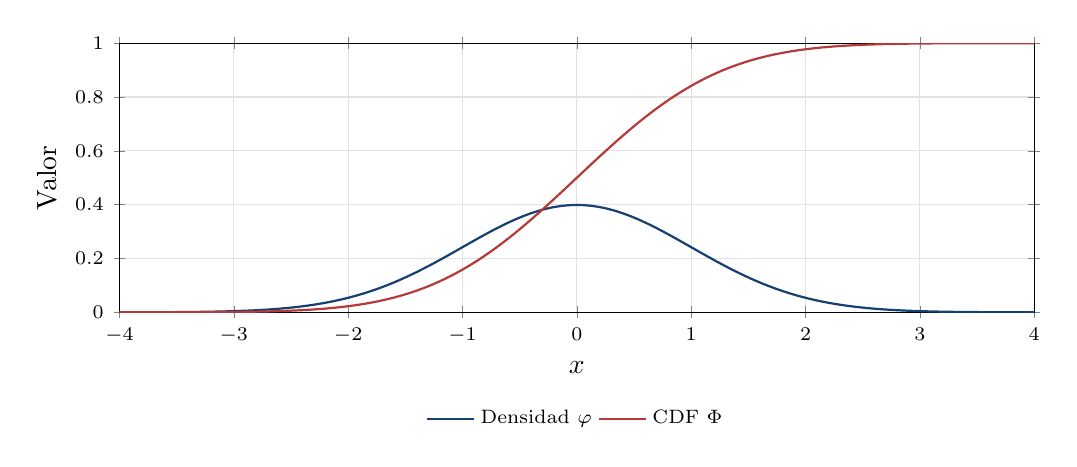
\begin{tikzpicture}\begin{axis}[base,axis lines=box,grid=major,minor tick num=0,width=13.2cm,height=5.0cm,xlabel={$x$},ylabel={Valor},legend style={at={(0.5,-0.32)},anchor=north,legend columns=2,font=\scriptsize,draw=none,fill=white}]
\addplot[thick,azul,] coordinates {(-4,0.0001338302258) (-3.933333333,0.0001743415784) (-3.866666667,0.0002261088384) (-3.8,0.0002919469258) (-3.733333333,0.0003752840237) (-3.666666667,0.0004802706516) (-3.6,0.0006119019301) (-3.533333333,0.0007761531062) (-3.466666667,0.0009801279613) (-3.4,0.001232219168) (-3.333333333,0.001542278996) (-3.266666667,0.001921797969) (-3.2,0.002384088201) (-3.133333333,0.00294446712) (-3.066666667,0.003620436228) (-3,0.004431848412) (-2.933333333,0.005401056181) (-2.866666667,0.006553032089) (-2.8,0.007915451583) (-2.733333333,0.009518727655) (-2.666666667,0.01139598602) (-2.6,0.01358296923) (-2.533333333,0.01611785811) (-2.466666667,0.01904099952) (-2.4,0.02239453029) (-2.333333333,0.02622188909) (-2.266666667,0.03056720973) (-2.2,0.03547459285) (-2.133333333,0.04098725605) (-2.066666667,0.04714656672) (-2,0.05399096651) (-1.933333333,0.06155480135) (-1.866666667,0.06986707607) (-1.8,0.0789501583) (-1.733333333,0.08881846109) (-1.666666667,0.09947713879) (-1.6,0.1109208347) (-1.533333333,0.123132522) (-1.466666667,0.1360824824) (-1.4,0.1497274656) (-1.333333333,0.1640100747) (-1.266666667,0.1788584165) (-1.2,0.194186055) (-1.133333333,0.2098922961) (-1.066666667,0.2258628275) (-1,0.2419707245) (-0.9333333333,0.2580778259) (-0.8666666667,0.2740364674) (-0.8,0.2896915528) (-0.7333333333,0.304882927) (-0.6666666667,0.3194480055) (-0.6,0.3332246029) (-0.5333333333,0.3460538932) (-0.4666666667,0.3577834292) (-0.4,0.3682701403) (-0.3333333333,0.3773832277) (-0.2666666667,0.3850068746) (-0.2,0.391042694) (-0.1333333333,0.3954118409) (-0.06666666667,0.3980567263) (0,0.3989422804) (0.06666666667,0.3980567263) (0.1333333333,0.3954118409) (0.2,0.391042694) (0.2666666667,0.3850068746) (0.3333333333,0.3773832277) (0.4,0.3682701403) (0.4666666667,0.3577834292) (0.5333333333,0.3460538932) (0.6,0.3332246029) (0.6666666667,0.3194480055) (0.7333333333,0.304882927) (0.8,0.2896915528) (0.8666666667,0.2740364674) (0.9333333333,0.2580778259) (1,0.2419707245) (1.066666667,0.2258628275) (1.133333333,0.2098922961) (1.2,0.194186055) (1.266666667,0.1788584165) (1.333333333,0.1640100747) (1.4,0.1497274656) (1.466666667,0.1360824824) (1.533333333,0.123132522) (1.6,0.1109208347) (1.666666667,0.09947713879) (1.733333333,0.08881846109) (1.8,0.0789501583) (1.866666667,0.06986707607) (1.933333333,0.06155480135) (2,0.05399096651) (2.066666667,0.04714656672) (2.133333333,0.04098725605) (2.2,0.03547459285) (2.266666667,0.03056720973) (2.333333333,0.02622188909) (2.4,0.02239453029) (2.466666667,0.01904099952) (2.533333333,0.01611785811) (2.6,0.01358296923) (2.666666667,0.01139598602) (2.733333333,0.009518727655) (2.8,0.007915451583) (2.866666667,0.006553032089) (2.933333333,0.005401056181) (3,0.004431848412) (3.066666667,0.003620436228) (3.133333333,0.00294446712) (3.2,0.002384088201) (3.266666667,0.001921797969) (3.333333333,0.001542278996) (3.4,0.001232219168) (3.466666667,0.0009801279613) (3.533333333,0.0007761531062) (3.6,0.0006119019301) (3.666666667,0.0004802706516) (3.733333333,0.0003752840237) (3.8,0.0002919469258) (3.866666667,0.0002261088384) (3.933333333,0.0001743415784) (4,0.0001338302258)};
\addlegendentry{Densidad $\varphi$}
\addplot[thick,rojo,] coordinates {(-4,3.167124183e-05) (-3.933333333,4.188796689e-05) (-3.866666667,5.516653503e-05) (-3.8,7.234804393e-05) (-3.733333333,9.44811248e-05) (-3.666666667,0.00012286639) (-3.6,0.0001591085902) (-3.533333333,0.0002051773657) (-3.466666667,0.0002634774656) (-3.4,0.0003369292657) (-3.333333333,0.0004290603332) (-3.266666667,0.0005441086525) (-3.2,0.0006871379379) (-3.133333333,0.0008641652091) (-3.066666667,0.001082300481) (-3,0.001349898032) (-2.933333333,0.001676718227) (-2.866666667,0.002074098364) (-2.8,0.00255513033) (-2.733333333,0.003134842261) (-2.666666667,0.003830380568) (-2.6,0.004661188024) (-2.533333333,0.005649172756) (-2.466666667,0.00681886227) (-2.4,0.008197535925) (-2.333333333,0.009815328629) (-2.266666667,0.01170529808) (-2.2,0.01390344751) (-2.133333333,0.01644869582) (-2.066666667,0.01938278709) (-2,0.02275013195) (-1.933333333,0.02659757402) (-1.866666667,0.03097407571) (-1.8,0.03593031911) (-1.733333333,0.04151821969) (-1.666666667,0.04779035227) (-1.6,0.0547992917) (-1.533333333,0.06259687279) (-1.466666667,0.07123337741) (-1.4,0.08075665923) (-1.333333333,0.09121121973) (-1.266666667,0.1026372518) (-1.2,0.1150696702) (-1.133333333,0.1285371493) (-1.066666667,0.1430611922) (-1,0.1586552539) (-0.9333333333,0.1753239449) (-0.8666666667,0.1930623371) (-0.8,0.2118553986) (-0.7333333333,0.2316775746) (-0.6666666667,0.2524925375) (-0.6,0.2742531178) (-0.5333333333,0.2969014286) (-0.4666666667,0.3203691909) (-0.4,0.3445782584) (-0.3333333333,0.3694413402) (-0.2666666667,0.3948629105) (-0.2,0.4207402906) (-0.1333333333,0.4469648834) (-0.06666666667,0.4734235357) (0,0.5) (0.06666666667,0.5265764643) (0.1333333333,0.5530351166) (0.2,0.5792597094) (0.2666666667,0.6051370895) (0.3333333333,0.6305586598) (0.4,0.6554217416) (0.4666666667,0.6796308091) (0.5333333333,0.7030985714) (0.6,0.7257468822) (0.6666666667,0.7475074625) (0.7333333333,0.7683224254) (0.8,0.7881446014) (0.8666666667,0.8069376629) (0.9333333333,0.8246760551) (1,0.8413447461) (1.066666667,0.8569388078) (1.133333333,0.8714628507) (1.2,0.8849303298) (1.266666667,0.8973627482) (1.333333333,0.9087887803) (1.4,0.9192433408) (1.466666667,0.9287666226) (1.533333333,0.9374031272) (1.6,0.9452007083) (1.666666667,0.9522096477) (1.733333333,0.9584817803) (1.8,0.9640696809) (1.866666667,0.9690259243) (1.933333333,0.973402426) (2,0.9772498681) (2.066666667,0.9806172129) (2.133333333,0.9835513042) (2.2,0.9860965525) (2.266666667,0.9882947019) (2.333333333,0.9901846714) (2.4,0.9918024641) (2.466666667,0.9931811377) (2.533333333,0.9943508272) (2.6,0.995338812) (2.666666667,0.9961696194) (2.733333333,0.9968651577) (2.8,0.9974448697) (2.866666667,0.9979259016) (2.933333333,0.9983232818) (3,0.998650102) (3.066666667,0.9989176995) (3.133333333,0.9991358348) (3.2,0.9993128621) (3.266666667,0.9994558913) (3.333333333,0.9995709397) (3.4,0.9996630707) (3.466666667,0.9997365225) (3.533333333,0.9997948226) (3.6,0.9998408914) (3.666666667,0.9998771336) (3.733333333,0.9999055189) (3.8,0.999927652) (3.866666667,0.9999448335) (3.933333333,0.999958112) (4,0.9999683288)};
\addlegendentry{CDF $\Phi$}
\end{axis}\end{tikzpicture}
\caption{La densidad mide masa por unidad; la CDF acumula área. Una tiene máximo en cero y la otra es creciente. Sus unidades y sus formas no son intercambiables.}\label{fig:cdf-1}\end{figure}

\section{CDF, supervivencia, densidad y cuantiles}
Una variable continua con densidad $f\ge0$, $\int_\R f=1$, satisface
\[
F(x)=\Pr(X\le x)=\int_{-\infty}^x f,\quad
S(x)=\Pr(X>x)=1-F(x),\quad F'=f.
\]
Si $a<b$, $\Pr(a<X\le b)=F(b)-F(a)=S(a)-S(b)$. Las dos restas son iguales en aritmética exacta; en una cola derecha, restar supervivencias puede retener muchos más dígitos.

El cuantil generalizado es $F^{-1}(p)=\inf\{x:F(x)\ge p\}$ para $0<p<1$. Si $F$ es estrictamente creciente y continua, resuelve $F(x)=p$. Diferenciando donde $f>0$,
\[
\frac{\dd F^{-1}(p)}{\dd p}=\frac1{f(F^{-1}(p))}.
\]
Cuando la densidad es diminuta, un error pequeño en probabilidad puede causar un error grande en $x$. Es una propiedad del problema inverso, no necesariamente del algoritmo.

La tasa de riesgo es $h(x)=f(x)/S(x)$ para $S(x)>0$. Como $S'=-f$,
\[
\frac{\dd}{\dd x}\log S(x)=-h(x).
\]
Trabajar con $\log S$ evita subdesbordamiento y cambia la métrica de error que debemos estudiar.

\section{Gamma, beta y F: por qué se repiten dos integrales}
Para $a>0$ definimos
\[
\Gamma(a)=\int_0^\infty t^{a-1}e^{-t}\dd t.
\]
Cerca de cero domina $t^{a-1}$, integrable cuando $a>0$; en infinito domina el exponencial. Integrando por partes,
$\Gamma(a+1)=a\Gamma(a)$, y $\Gamma(1)=1$, por lo que $\Gamma(n+1)=n!$. El cambio $t=s^2$ da $\Gamma(1/2)=\sqrt\pi$.

Si $X$ tiene forma $a$ y tasa $\lambda>0$,
\[
f_X(x)=\frac{\lambda^a}{\Gamma(a)}x^{a-1}e^{-\lambda x}\ind_{\{x>0\}},
\qquad F_X(x)=P(a,\lambda x),
\]
donde $P(a,z)=\Gamma(a)^{-1}\int_0^z t^{a-1}e^{-t}\dd t$. Su complemento $Q(a,z)$ integra desde $z$ hasta infinito.

Para $a,b>0$,
\[
B(a,b)=\int_0^1 t^{a-1}(1-t)^{b-1}\dd t
=\frac{\Gamma(a)\Gamma(b)}{\Gamma(a+b)},\quad
I_x(a,b)=\frac1{B(a,b)}\int_0^x t^{a-1}(1-t)^{b-1}\dd t.
\]
La identidad para $B$ usa $u=rs$, $v=r(1-s)$ en $\Gamma(a)\Gamma(b)$; el jacobiano es $r$ y la integral se separa en $\Gamma(a+b)B(a,b)$.

Una chi cuadrado de $\nu$ grados de libertad es gamma con forma $\nu/2$ y tasa $1/2$. Para chi cuadrados independientes $U,V$ con grados $d_1,d_2$,
\[
W=\frac{U/d_1}{V/d_2},\qquad
\Pr(W\le w)=I_{\frac{d_1w}{d_1w+d_2}}\left(\frac{d_1}2,\frac{d_2}2\right).
\]
La deducción por transformación de densidades vendrá después. Un buen evaluador beta resuelve así varias distribuciones a la vez.

\section{Mapa histórico y mapa lógico}
Las técnicas no surgieron como una única cadena destinada exclusivamente a la normal. Interpolación, tablas, integración de ecuaciones diferenciales y teoría de aproximación tienen historias propias. El trabajo de Gauss de 1814 sobre integración aproximada constituye un hito: mover los nodos permite obtener exactitud polinómica muy elevada con pocas evaluaciones.

\begin{center}\small
\begin{tabular}{>{\raggedright\arraybackslash}p{2cm}>{\raggedright\arraybackslash}p{5.3cm}>{\raggedright\arraybackslash}p{7.3cm}}
\toprule Hito & Idea matemática & Papel numérico\\\midrule
Gauss, 1814 & Nodos libres y exactitud elevada & Integrar en intervalos transformados\\
Siglo XIX & Ortogonalidad y fracciones continuas & Relacionar momentos, ceros y cocientes\\
Padé, 1892 & Ajustar una serie mediante cocientes & Representar polos y comportamientos no polinómicos\\
Remez, década de 1930 & Intercambio de extremos del error & Aproximación uniforme de bajo grado\\
Golub--Welsch, 1969 & Matriz tridiagonal simétrica & Calcular nodos y pesos\\
Cody, 1969 & Aproximación racional de la función error & Evaluación rápida por regiones\\
Takahasi--Mori, 1974 & Transformación doble exponencial & Integrandos con extremos difíciles\\
Wichura, 1988 & Aproximación racional del cuantil normal & Invertir probabilidades\\
DiDonato--Morris, 1992 & Algoritmos de beta incompleta & Distribuciones beta, F y binomial\\
AAA, desde 2018 & Forma baricéntrica adaptativa & Aproximantes a partir de muestras\\
\bottomrule
\end{tabular}
\end{center}
La fecha de un hito no significa que toda biblioteca actual use ese método ni que sustituya universalmente al anterior. Hoy conviven series, cuadraturas, fracciones continuas, expansiones uniformes y aritmética ampliada. Elegir región y escala es parte del algoritmo.

\parte{II. El error: lo que una fórmula exacta no revela}
\section{Tres errores y una desigualdad triangular}
Sea $I$ una integral exacta, $I_B$ su versión truncada, $\mathcal Q_n$ una regla en aritmética real y $\widehat{\mathcal Q}_n$ el resultado de computadora. Insertando cantidades intermedias,
\[
|I-\widehat{\mathcal Q}_n|
\le |I-I_B|+|I_B-\mathcal Q_n|+|\mathcal Q_n-\widehat{\mathcal Q}_n|.
\]
Son errores de dominio, discretización y redondeo. Una serie añade error por detenerla y un racional añade error de aproximación. Si la entrada $x$ llega perturbada, hay otro término $|F(x)-F(\widehat x)|$. Pedir tolerancia $\tau$ requiere presupuestos cuya suma no supere $\tau$, cuando contamos con cotas válidas.

El error absoluto es $|\widehat y-y|$ y el relativo es $|\widehat y-y|/|y|$, si $y\ne0$. Para $y=10^{-100}$, un error absoluto de $10^{-16}$ no garantiza ninguna cifra significativa. Un error pequeño en una CDF cercana a uno puede coexistir con un error relativo enorme en su complemento. Por eso un evaluador debe ofrecer la cola pequeña directamente.

\section{La aritmética flotante desde su representación}
Un sistema binario normalizado representa
\[
\pm(1.b_1b_2\cdots b_{p-1})_2\,2^e.
\]
Hay un número finito de bits y de exponentes. En el rango normal, redondeando al más cercano,
\[
\fl(x)=x(1+\delta),\quad |\delta|\le u,\quad u=2^{-p}.
\]
Para binary64, $p=53$, $u=2^{-53}\approx1.11\,10^{-16}$. La distancia entre uno y el siguiente número mayor es $2^{-52}=2u$: no debemos confundir ambas convenciones de epsilon de máquina.

Si no hay desbordamiento ni problemas de subnormalidad,
\[
\fl(a\circ b)=(a\circ b)(1+\delta),\quad |\delta|\le u,
\qquad \circ\in\{+,-,\times,/\}.
\]
Una resta de valores cercanos puede ser exacta como operación y revelar errores anteriores. Los subnormales tienen espaciado aproximadamente constante y allí falla la cota relativa uniforme. Un exponencial puede redondear a cero aunque su logaritmo siga siendo perfectamente representable.

\section{Condicionamiento: dificultad del problema}
Para $y=f(x)\ne0$ y $x\ne0$, a primer orden,
\[
\frac{\Delta y}{y}\approx\frac{xf'(x)}{f(x)}\frac{\Delta x}x,
\qquad \kappa_f(x)=\left|\frac{xf'(x)}{f(x)}\right|.
\]
Este número mide sensibilidad de la respuesta exacta, no calidad del algoritmo. Para la cola normal,
\[
\kappa_{\Q}(x)=\frac{|x|\ph(x)}{\Q(x)}\sim x^2\quad(x\to\infty).
\]
La relación asintótica será deducida con integración por partes. En $x=0$ se usa sensibilidad absoluta, $|f'(0)|$, porque perturbación relativa de una entrada nula no tiene sentido.

Si $g(x)=\log\Q(x)$, $g'=-\ph/\Q$. Un error $\Delta g$ significa un factor multiplicativo $e^{\Delta g}$ en la cola. Si una matriz $A$ está casi singular, los coeficientes de un interpolante resueltos por $Ac=b$ pueden ser muy sensibles; cambiar de base puede evitar una dificultad aritmética que no pertenece a la función aproximada.

\section{Estabilidad y cancelación: la resta que engaña}
Un algoritmo es estable hacia atrás si entrega la respuesta exacta de datos ligeramente perturbados. Un problema bien condicionado más un algoritmo estable suele producir error pequeño hacia adelante.

Para $x>0$ pequeño,
\[
1-e^{-x}=x-\frac{x^2}2+\frac{x^3}6-\cdots.
\]
Si el exponencial tiene error absoluto aproximadamente $u$, la resta hereda error relativo $u/x$. Una operación especializada, $-\expmone(-x)$, evalúa directamente esa diferencia. De forma análoga, $\logonep(x)$ evalúa $\log(1+x)$ sin perder $x$ al sumarlo a uno.

Para $\ell\le0$, una forma estable es
\[
\log(1-e^\ell)=
\begin{cases}
\logonep(-e^\ell),&\ell<-\log2,\\
\log(-\expmone(\ell)),&-\log2\le\ell<0.
\end{cases}
\]
Para $\ell=0$ el valor límite es $-\infty$. Las ramas representan la misma función y evitan restas peligrosas en regiones diferentes.






\begin{figure}[htbp]\centering
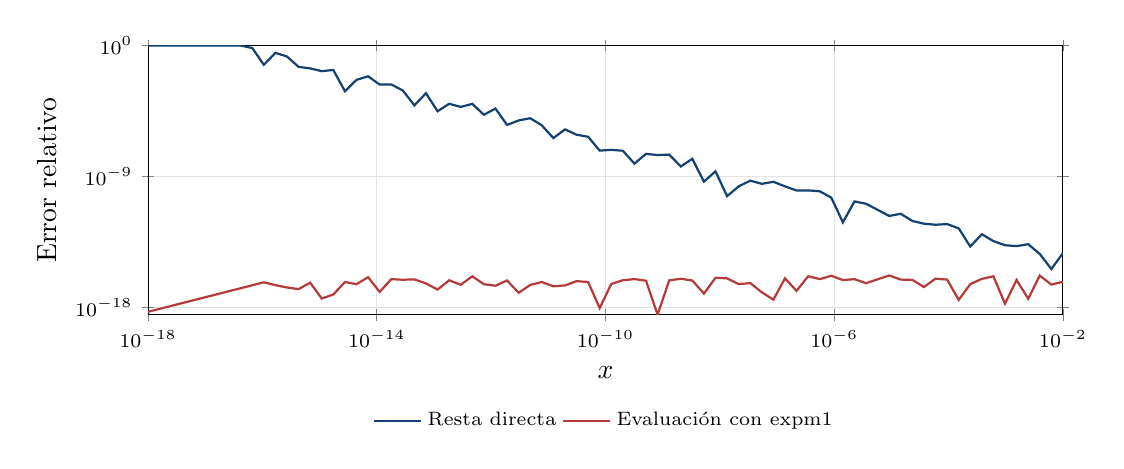
\begin{tikzpicture}\begin{axis}[base,axis lines=box,grid=major,minor tick num=0,width=13.2cm,height=5.0cm,xmode=log,ymode=log,xlabel={$x$},ylabel={Error relativo},unbounded coords=discard,xtick={1e-18,1e-14,1e-10,1e-6,1e-2},legend style={at={(0.5,-0.32)},anchor=north,legend columns=2,font=\scriptsize,draw=none,fill=white}]
\addplot[thick,azul,] coordinates {(1e-18,1) (1.594159037e-18,1) (2.541343037e-18,1) (4.051304969e-18,1) (6.45842443e-18,1) (1.029575567e-17,1) (1.641307195e-17,1) (2.616504699e-17,1) (4.171124612e-17,1) (6.649435997e-17,0.6696499149) (1.060025849e-16,0.04735467147) (1.689849787e-16,0.313990194) (2.69388931e-16,0.1757471098) (4.294487989e-16,0.03409116758) (6.846096839e-16,0.02698744923) (1.091376715e-15,0.01726838196) (1.739828053e-15,0.02099563023) (2.773562614e-15,0.0007192725177) (4.421499907e-15,0.004385885227) (7.048574036e-15,0.00768509787) (1.1236548e-14,0.002073185882) (1.791284455e-14,0.002135554164) (2.855592302e-14,0.0008121357877) (4.552268276e-14,7.773587202e-05) (7.257039612e-14,0.0005262433346) (1.156887528e-13,3.037171371e-05) (1.844262709e-13,9.882793928e-05) (2.940048064e-13,6.037150515e-05) (4.686904192e-13,9.759483778e-05) (7.471670676e-13,1.743651021e-05) (1.191103133e-12,4.630148011e-05) (1.898807824e-12,3.483529434e-06) (3.027001654e-12,7.077261285e-06) (4.825522043e-12,1.008978892e-05) (7.692649575e-12,3.283592224e-06) (1.226330684e-11,4.367741845e-07) (1.954966143e-11,1.727155126e-06) (3.116526945e-11,7.418530106e-07) (4.968239595e-11,5.357317398e-07) (7.92016405e-11,5.989058749e-08) (1.26260011e-10,6.752986499e-08) (2.012785376e-10,5.871711588e-08) (3.208699997e-10,7.62474078e-09) (5.115178099e-10,3.57681877e-08) (8.154407395e-10,2.97191031e-08) (1.299942224e-09,3.1828012e-08) (2.072314645e-09,4.893184887e-09) (3.30359912e-09,1.62531532e-08) (5.266462393e-09,4.385463689e-10) (8.39557862e-09,2.270540586e-09) (1.338388753e-08,4.411986682e-11) (2.133604527e-08,2.081622976e-10) (3.401304938e-08,5.157337615e-10) (5.422221007e-08,3.128199687e-10) (8.643882621e-08,4.287343192e-10) (1.37797236e-07,2.095211709e-10) (2.196707091e-07,1.083933753e-10) (3.501900461e-07,1.104240849e-10) (5.582586269e-07,9.626284856e-11) (8.899530353e-07,3.51216067e-11) (1.418726674e-06,7.01408975e-13) (2.261675949e-06,1.919366516e-11) (3.605471154e-06,1.331538049e-11) (5.747694425e-06,5.087447547e-12) (9.162739012e-06,1.935626266e-12) (1.46068632e-05,2.720303398e-12) (2.328566298e-05,8.727869741e-13) (3.712105009e-05,5.682612059e-13) (5.917685748e-05,4.809555347e-13) (9.433732216e-05,5.325003234e-13) (0.0001503886947,2.730430681e-13) (0.0002397434968,1.522823366e-14) (0.0003821892621,1.073891293e-13) (0.0006092704661,3.609208041e-14) (0.0009712740198,1.885219262e-14) (0.001548365257,1.630024829e-14) (0.002468340467,2.219194683e-14) (0.003934927263,4.73774451e-15) (0.006272899858,4.368790878e-16) (0.01,5.369366971e-15)};
\addlegendentry{Resta directa}
\addplot[thick,rojo,] coordinates {(1e-18,5e-19) (1.594159037e-18,7.970795187e-19) (2.541343037e-18,1.270671518e-18) (4.051304969e-18,2.025652485e-18) (6.45842443e-18,3.229212215e-18) (1.029575567e-17,5.147877837e-18) (1.641307195e-17,8.206535977e-18) (2.616504699e-17,1.308252349e-17) (4.171124612e-17,2.085562306e-17) (6.649435997e-17,3.324717998e-17) (1.060025849e-16,5.300129244e-17) (1.689849787e-16,3.386122562e-17) (2.69388931e-16,2.333131521e-17) (4.294487989e-16,1.813223041e-17) (6.846096839e-16,5.016757786e-17) (1.091376715e-15,4.075983388e-18) (1.739828053e-15,7.75986274e-18) (2.773562614e-15,5.54071546e-17) (4.421499907e-15,3.954104243e-17) (7.048574036e-15,1.193430003e-16) (1.1236548e-14,1.156987838e-17) (1.791284455e-14,8.736748245e-17) (2.855592302e-14,7.983038192e-17) (4.552268276e-14,8.441236671e-17) (7.257039612e-14,4.4524998e-17) (1.156887528e-13,1.680168401e-17) (1.844262709e-13,7.306610139e-17) (2.940048064e-13,3.600926509e-17) (4.686904192e-13,1.379278468e-16) (7.471670676e-13,3.923278251e-17) (1.191103133e-12,3.078066119e-17) (1.898807824e-12,7.140118255e-17) (3.027001654e-12,1.00740154e-17) (4.825522043e-12,3.492006176e-17) (7.692649575e-12,5.573383582e-17) (1.226330684e-11,2.832412718e-17) (1.954966143e-11,3.227832936e-17) (3.116526945e-11,6.385574455e-17) (4.968239595e-11,5.568342791e-17) (7.92016405e-11,8.962527617e-19) (1.26260011e-10,4.108145174e-17) (2.012785376e-10,7.375261168e-17) (3.208699997e-10,8.838507635e-17) (5.115178099e-10,6.82579062e-17) (8.154407395e-10,3.153126618e-19) (1.299942224e-09,7.157249871e-17) (2.072314645e-09,9.308981203e-17) (3.30359912e-09,7.045430247e-17) (5.266462393e-09,8.85742944e-18) (8.39557862e-09,1.091489573e-16) (1.338388753e-08,9.948738626e-17) (2.133604527e-08,3.953050127e-17) (3.401304938e-08,4.703863014e-17) (5.422221007e-08,1.102942788e-17) (8.643882621e-08,3.396947734e-18) (1.37797236e-07,9.984114819e-17) (2.196707091e-07,1.367165127e-17) (3.501900461e-07,1.387857443e-16) (5.582586269e-07,8.838494154e-17) (8.899530353e-07,1.499171848e-16) (1.418726674e-06,7.536084464e-17) (2.261675949e-06,8.764186981e-17) (3.605471154e-06,4.611457182e-17) (5.747694425e-06,8.527448308e-17) (9.162739012e-06,1.574815628e-16) (1.46068632e-05,8.150951244e-17) (2.328566298e-05,7.787214024e-17) (3.712105009e-05,2.529152764e-17) (5.917685748e-05,9.45502213e-17) (9.433732216e-05,8.178340472e-17) (0.0001503886947,3.304413735e-18) (0.0002397434968,3.991249114e-17) (0.0003821892621,9.1935312e-17) (0.0006092704661,1.365017202e-16) (0.0009712740198,1.808261561e-18) (0.001548365257,7.704973576e-17) (0.002468340467,3.947394037e-18) (0.003934927263,1.543211418e-16) (0.006272899858,3.708802157e-17) (0.01,5.767802896e-17)};
\addlegendentry{Evaluación con expm1}
\end{axis}\end{tikzpicture}
\caption{Cancelación en $1-e^{-x}$. La comparación usa una referencia decimal ampliada para los mismos argumentos representables. La operación especializada conserva precisión cuando la resta directa redondea a cero.}\label{fig:cdf-2}\end{figure}

\section{Errores de suma y acumulación compensada}
Definamos $\gamma_n=nu/(1-nu)$ para $nu<1$. Productos de factores $1+\delta_i$ con $|\delta_i|\le u$ se pueden escribir $1+\theta_n$, $|\theta_n|\le\gamma_n$. Una suma secuencial satisface
\[
\left|\fl\left(\sum_{i=1}^n a_i\right)-\sum_{i=1}^n a_i\right|
\le\gamma_{n-1}\sum_{i=1}^n|a_i|.
\]
El cociente $\sum|a_i|/|\sum a_i|$ describe cancelación. Para términos positivos vale uno; para una suma alternante casi nula puede ser enorme.

Sumar por pares reduce la profundidad a $O(\log n)$. La compensación guarda cantidades perdidas:
\begin{lstlisting}
s = 0; c = 0
for a in terms:
    y = a - c
    t = s + y
    c = (t - s) - y
    s = t
\end{lstlisting}
La compensación mejora acumulación, pero no arregla una serie intrínsecamente mal condicionada ni recupera términos que ya subdesbordaron. Reorganizar una fórmula suele ser más poderoso que sumar la misma fórmula con más cuidado.

\section{Polinomios como vectores y Horner}
Un polinomio $p(x)=c_0+c_1x+\cdots+c_mx^m$ pertenece al espacio $\mathcal P_m$, de dimensión $m+1$. La base monomial es $1,x,\ldots,x^m$; otra base puede ser ortogonal. El vector $c$ contiene coordenadas, no valores de la función.

Horner reagrupa
\[
p(x)=c_0+x(c_1+x(c_2+\cdots+xc_m)).
\]
Con $b_m=c_m$, $b_k=c_k+xb_{k+1}$, obtenemos $p=b_0$ mediante $m$ productos y $m$ sumas. Por sustitución descendente se prueba la identidad. Una cota habitual es
\[
|\widehat p(x)-p(x)|\le\gamma_{2m}\sum_{k=0}^m|c_k||x|^k.
\]
Cerca de una raíz el error relativo puede seguir siendo grande. Una operación producto-suma fusionada redondea $ab+c$ una vez y reduce acumulación, pero no cambia la sensibilidad intrínseca.

\section{Interpolación de Lagrange desde las condiciones}
Dados nodos distintos $x_0,\ldots,x_m$, buscamos $p(x_i)=y_i$ con $p\in\mathcal P_m$. La matriz de monomios es
\[
V=\begin{pmatrix}1&x_0&\cdots&x_0^m\\1&x_1&\cdots&x_1^m\\
\vdots&\vdots&&\vdots\\1&x_m&\cdots&x_m^m\end{pmatrix},\qquad Vc=y.
\]
Su determinante es $\prod_{i<j}(x_j-x_i)\ne0$. También hay una prueba sin determinantes: dos interpolantes distintos tendrían una diferencia de grado a lo sumo $m$ con $m+1$ raíces, imposible.

Construimos
\[
\ell_i(x)=\prod_{j\ne i}\frac{x-x_j}{x_i-x_j},
\quad \ell_i(x_j)=\delta_{ij},
\quad p(x)=\sum_{i=0}^m y_i\ell_i(x).
\]
Interpolar la constante uno da $\sum_i\ell_i=1$. Para dos nodos, obtenemos la recta
$p(x)=y_0(x_1-x)/(x_1-x_0)+y_1(x-x_0)/(x_1-x_0)$.
Los pesos de cuadratura surgirán integrando cada $\ell_i$.

\section{El resto de interpolación, demostrado}
Sea $\omega(t)=\prod_{i=0}^m(t-x_i)$. Para $x$ fuera de los nodos, definimos
$K=[f(x)-p(x)]/\omega(x)$ y $g(t)=f(t)-p(t)-K\omega(t)$. Tiene ceros en los nodos y en $x$. Aplicando Rolle $m+1$ veces,
\[
0=g^{(m+1)}(\xi)=f^{(m+1)}(\xi)-K(m+1)!.
\]
Así,
\[
f(x)-p(x)=\frac{f^{(m+1)}(\xi_x)}{(m+1)!}\prod_{i=0}^m(x-x_i).
\]
En los nodos el error es cero. Si $|f^{(m+1)}|\le M$, podemos acotar el error con $\max|\omega|$. El punto $\xi_x$ depende de $x$: sacarlo de una integral requiere justificar signo y continuidad.

Aumentar el grado no garantiza mejorar. Los polinomios cardinales pueden amplificar perturbaciones y el producto nodal puede crecer en extremos. Elegir nodos es parte del método.

\section{Forma baricéntrica y constante de Lebesgue}
Definimos $\lambda_i=[\prod_{j\ne i}(x_i-x_j)]^{-1}$. Como
$\ell_i=\lambda_i\omega/(x-x_i)$ y $\sum\ell_i=1$,
\[
p(x)=\frac{\sum_i\lambda_i y_i/(x-x_i)}
{\sum_i\lambda_i/(x-x_i)}.
\]
En un nodo se devuelve $y_i$. Escalar todos los $\lambda_i$ por la misma constante conserva el cociente. Para estos pesos, la expresión racional se simplifica al mismo polinomio; con pesos diferentes puede ser una función racional genuina.

La función de Lebesgue es $\Lambda_m(x)=\sum|\ell_i(x)|$. Si $|\Delta y_i|\le\eta$,
\[
|\Delta p(x)|\le\eta\Lambda_m(x).
\]
Con $\Lambda_m=\max\Lambda_m(x)$ y cualquier $q\in\mathcal P_m$,
\[
\norm{f-p}_\infty\le(1+\Lambda_m)\norm{f-q}_\infty.
\]
Se obtiene sumando y restando $q$ y usando que interpolar $q$ lo conserva. La cota separa aproximabilidad de $f$ y amplificación introducida por los nodos.

\section{Diferencias divididas y forma de Newton}
Definimos $f[x_i]=f(x_i)$ y
\[
f[x_i,\ldots,x_{i+k}]
=\frac{f[x_{i+1},\ldots,x_{i+k}]-f[x_i,\ldots,x_{i+k-1}]}
{x_{i+k}-x_i}.
\]
Entonces
\[
p_m(x)=f[x_0]+f[x_0,x_1](x-x_0)+\cdots+
f[x_0,\ldots,x_m]\prod_{j=0}^{m-1}(x-x_j).
\]
Agregar un nodo requiere un término. Si los nodos se aproximan, las diferencias divididas tienden a derivadas divididas por factoriales, con suavidad suficiente. El polinomio exacto no depende del orden, pero su evaluación flotante sí puede hacerlo.

\begin{ejemplo}[Tres valores de la exponencial]
En $0,1,2$, las primeras diferencias son $e-1$ y $e^2-e$, y la segunda $(e^2-2e+1)/2$:
\[
p_2(x)=1+(e-1)x+\frac{(e-1)^2}2x(x-1).
\]
En $x=1/2$, el resto está acotado por
$e^2|(1/2)(-1/2)(-3/2)|/6=e^2/16$. La cota es rigurosa pero conservadora.
\end{ejemplo}

\section{Runge, singularidades y división del dominio}
La función $f(x)=1/(1+25x^2)$ es suave en $[-1,1]$ pero tiene polos complejos próximos al intervalo. Interpolantes de grado creciente en nodos equiespaciados pueden oscilar cerca de $\pm1$. Exactitud en nodos no impone exactitud entre ellos.

Los nodos de Chebyshev agrupan evaluaciones en extremos:
\[
x_j=\cos(j\pi/m),\qquad j=0,\ldots,m.
\]
La distancia de las singularidades complejas gobierna la rapidez de aproximación polinómica para funciones analíticas. Una función entera como $e^{-x^2}$ tiene otro comportamiento. Esta conexión será precisada con elipses de Bernstein.

Un algoritmo moderno divide dominios y transforma variables. Un polinomio pequeño en cada región suele ser mejor que uno gigantesco para cubrir centro, transición y cola infinita. Los criterios de división deben conservar continuidad y controlar el error a ambos lados de cada frontera.







\begin{figure}[htbp]\centering
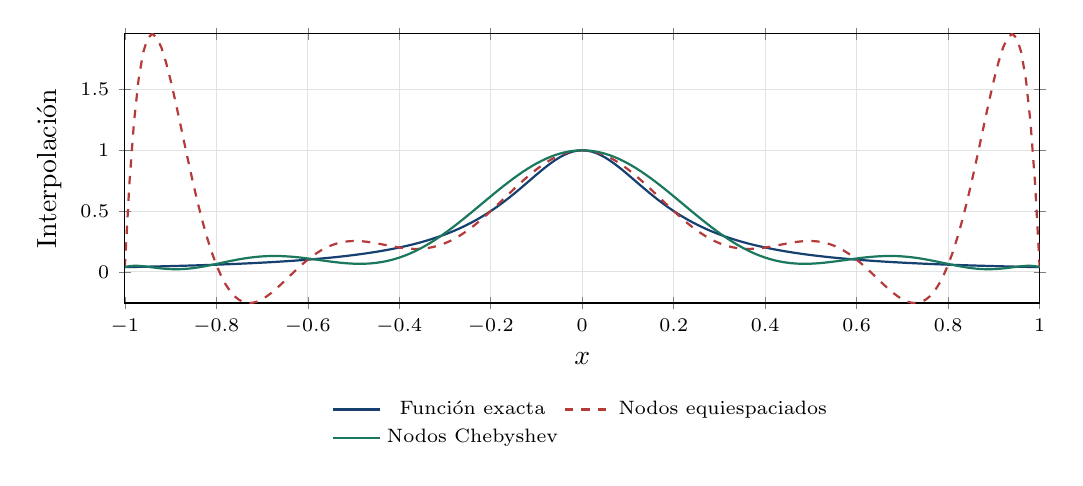
\begin{tikzpicture}\begin{axis}[base,axis lines=box,grid=major,minor tick num=0,width=13.2cm,height=5.0cm,xlabel={$x$},ylabel={Interpolación},legend style={at={(0.5,-0.32)},anchor=north,legend columns=2,font=\scriptsize,draw=none,fill=white}]
\addplot[thick,azul,] coordinates {(-1,0.03846153846) (-0.99,0.03921184198) (-0.98,0.0399840064) (-0.97,0.04077887654) (-0.96,0.04159733777) (-0.95,0.0424403183) (-0.94,0.04330879168) (-0.93,0.04420377942) (-0.92,0.04512635379) (-0.91,0.04607764082) (-0.9,0.04705882353) (-0.89,0.0480711453) (-0.88,0.04911591356) (-0.87,0.0501945037) (-0.86,0.05130836326) (-0.85,0.05245901639) (-0.84,0.05364806867) (-0.83,0.05487721224) (-0.82,0.05614823133) (-0.81,0.05746300819) (-0.8,0.05882352941) (-0.79,0.06023189279) (-0.78,0.06169031462) (-0.77,0.06320113762) (-0.76,0.06476683938) (-0.75,0.06639004149) (-0.74,0.0680735194) (-0.73,0.06982021295) (-0.72,0.07163323782) (-0.71,0.07351589781) (-0.7,0.07547169811) (-0.69,0.07750435962) (-0.68,0.07961783439) (-0.67,0.08181632236) (-0.66,0.08410428932) (-0.65,0.08648648649) (-0.64,0.08896797153) (-0.63,0.09155413138) (-0.62,0.09425070688) (-0.61,0.09706381946) (-0.6,0.1) (-0.59,0.10306622) (-0.58,0.1062699256) (-0.57,0.1096190737) (-0.56,0.1131221719) (-0.55,0.1167883212) (-0.54,0.1206272618) (-0.53,0.1246494235) (-0.52,0.1288659794) (-0.51,0.1332889037) (-0.5,0.1379310345) (-0.49,0.1428061407) (-0.48,0.1479289941) (-0.47,0.1533154465) (-0.46,0.1589825119) (-0.45,0.1649484536) (-0.44,0.1712328767) (-0.43,0.1778568253) (-0.42,0.1848428835) (-0.41,0.1922152811) (-0.4,0.2) (-0.39,0.2082248829) (-0.38,0.2169197397) (-0.37,0.22611645) (-0.36,0.2358490566) (-0.35,0.2461538462) (-0.34,0.2570694087) (-0.33,0.2686366689) (-0.32,0.2808988764) (-0.31,0.293901543) (-0.3,0.3076923077) (-0.29,0.3223207091) (-0.28,0.3378378378) (-0.27,0.354295837) (-0.26,0.3717472119) (-0.25,0.3902439024) (-0.24,0.4098360656) (-0.23,0.4305705059) (-0.22,0.4524886878) (-0.21,0.4756242568) (-0.2,0.5) (-0.19,0.5256241787) (-0.18,0.5524861878) (-0.17,0.5805515239) (-0.16,0.6097560976) (-0.15,0.64) (-0.14,0.6711409396) (-0.13,0.7029876977) (-0.12,0.7352941176) (-0.11,0.7677543186) (-0.1,0.8) (-0.09,0.8316008316) (-0.08,0.8620689655) (-0.07,0.8908685969) (-0.06,0.9174311927) (-0.05,0.9411764706) (-0.04,0.9615384615) (-0.03,0.97799511) (-0.02,0.9900990099) (-0.01,0.9975062344) (0,1) (0.01,0.9975062344) (0.02,0.9900990099) (0.03,0.97799511) (0.04,0.9615384615) (0.05,0.9411764706) (0.06,0.9174311927) (0.07,0.8908685969) (0.08,0.8620689655) (0.09,0.8316008316) (0.1,0.8) (0.11,0.7677543186) (0.12,0.7352941176) (0.13,0.7029876977) (0.14,0.6711409396) (0.15,0.64) (0.16,0.6097560976) (0.17,0.5805515239) (0.18,0.5524861878) (0.19,0.5256241787) (0.2,0.5) (0.21,0.4756242568) (0.22,0.4524886878) (0.23,0.4305705059) (0.24,0.4098360656) (0.25,0.3902439024) (0.26,0.3717472119) (0.27,0.354295837) (0.28,0.3378378378) (0.29,0.3223207091) (0.3,0.3076923077) (0.31,0.293901543) (0.32,0.2808988764) (0.33,0.2686366689) (0.34,0.2570694087) (0.35,0.2461538462) (0.36,0.2358490566) (0.37,0.22611645) (0.38,0.2169197397) (0.39,0.2082248829) (0.4,0.2) (0.41,0.1922152811) (0.42,0.1848428835) (0.43,0.1778568253) (0.44,0.1712328767) (0.45,0.1649484536) (0.46,0.1589825119) (0.47,0.1533154465) (0.48,0.1479289941) (0.49,0.1428061407) (0.5,0.1379310345) (0.51,0.1332889037) (0.52,0.1288659794) (0.53,0.1246494235) (0.54,0.1206272618) (0.55,0.1167883212) (0.56,0.1131221719) (0.57,0.1096190737) (0.58,0.1062699256) (0.59,0.10306622) (0.6,0.1) (0.61,0.09706381946) (0.62,0.09425070688) (0.63,0.09155413138) (0.64,0.08896797153) (0.65,0.08648648649) (0.66,0.08410428932) (0.67,0.08181632236) (0.68,0.07961783439) (0.69,0.07750435962) (0.7,0.07547169811) (0.71,0.07351589781) (0.72,0.07163323782) (0.73,0.06982021295) (0.74,0.0680735194) (0.75,0.06639004149) (0.76,0.06476683938) (0.77,0.06320113762) (0.78,0.06169031462) (0.79,0.06023189279) (0.8,0.05882352941) (0.81,0.05746300819) (0.82,0.05614823133) (0.83,0.05487721224) (0.84,0.05364806867) (0.85,0.05245901639) (0.86,0.05130836326) (0.87,0.0501945037) (0.88,0.04911591356) (0.89,0.0480711453) (0.9,0.04705882353) (0.91,0.04607764082) (0.92,0.04512635379) (0.93,0.04420377942) (0.94,0.04330879168) (0.95,0.0424403183) (0.96,0.04159733777) (0.97,0.04077887654) (0.98,0.0399840064) (0.99,0.03921184198) (1,0.03846153846)};
\addlegendentry{Función exacta}
\addplot[thick,rojo,dashed] coordinates {(-1,0.03846153846) (-0.99,0.7260710423) (-0.98,1.230316555) (-0.97,1.580987543) (-0.96,1.804385456) (-0.95,1.92363115) (-0.94,1.958951842) (-0.93,1.927948604) (-0.92,1.845845367) (-0.91,1.725720373) (-0.9,1.57872099) (-0.89,1.414262755) (-0.88,1.240213485) (-0.87,1.063063274) (-0.86,0.8880811461) (-0.85,0.7194591284) (-0.84,0.5604444446) (-0.83,0.4134605401) (-0.82,0.280217594) (-0.81,0.1618131571) (-0.8,0.05882352941) (-0.79,-0.02861353898) (-0.78,-0.1007242617) (-0.77,-0.1580318083) (-0.76,-0.2012963615) (-0.75,-0.2314617499) (-0.74,-0.2496081891) (-0.73,-0.2569106839) (-0.72,-0.2546026691) (-0.71,-0.2439444827) (-0.7,-0.2261962891) (-0.69,-0.2025950869) (-0.68,-0.1743354554) (-0.67,-0.1425537116) (-0.66,-0.1083151688) (-0.65,-0.07260420322) (-0.64,-0.03631685126) (-0.63,-0.0002556789873) (-0.62,0.03487332285) (-0.61,0.06846204744) (-0.6,0.1) (-0.59,0.1290726469) (-0.58,0.155358574) (-0.57,0.17862563) (-0.56,0.1987262168) (-0.55,0.2155918789) (-0.54,0.2292273301) (-0.53,0.2397040467) (-0.52,0.2471535451) (-0.51,0.2517604508) (-0.5,0.2537554573) (-0.49,0.2534082633) (-0.48,0.2510205687) (-0.47,0.2469192003) (-0.46,0.24144943) (-0.45,0.2349685431) (-0.44,0.2278397033) (-0.43,0.2204261574) (-0.42,0.2130858141) (-0.41,0.2061662263) (-0.4,0.2) (-0.39,0.1949006483) (-0.38,0.1911589022) (-0.37,0.1890394872) (-0.36,0.1887783689) (-0.35,0.1905804668) (-0.34,0.1946178332) (-0.33,0.2010282879) (-0.32,0.2099144991) (-0.31,0.2213434949) (-0.3,0.2353465913) (-0.29,0.2519197157) (-0.28,0.2710241055) (-0.27,0.2925873591) (-0.26,0.3165048155) (-0.25,0.3426412344) (-0.24,0.3708327529) (-0.23,0.4008890878) (-0.22,0.4325959573) (-0.21,0.4657176909) (-0.2,0.5) (-0.19,0.5351728774) (-0.18,0.5709535983) (-0.17,0.6070497917) (-0.16,0.6431625541) (-0.15,0.6789895773) (-0.14,0.7142282618) (-0.13,0.7485787894) (-0.12,0.7817471293) (-0.11,0.8134479523) (-0.1,0.8434074298) (-0.09,0.8713658956) (-0.08,0.8970803487) (-0.07,0.9203267787) (-0.06,0.9409022959) (-0.05,0.9586270487) (-0.04,0.973345916) (-0.03,0.9849299604) (-0.02,0.9932776317) (-0.01,0.9983157129) (0,1) (0.01,0.9983157129) (0.02,0.9932776317) (0.03,0.9849299604) (0.04,0.973345916) (0.05,0.9586270487) (0.06,0.9409022959) (0.07,0.9203267787) (0.08,0.8970803487) (0.09,0.8713658956) (0.1,0.8434074298) (0.11,0.8134479523) (0.12,0.7817471293) (0.13,0.7485787894) (0.14,0.7142282618) (0.15,0.6789895773) (0.16,0.6431625541) (0.17,0.6070497917) (0.18,0.5709535983) (0.19,0.5351728774) (0.2,0.5) (0.21,0.4657176909) (0.22,0.4325959573) (0.23,0.4008890878) (0.24,0.3708327529) (0.25,0.3426412344) (0.26,0.3165048155) (0.27,0.2925873591) (0.28,0.2710241055) (0.29,0.2519197157) (0.3,0.2353465913) (0.31,0.2213434949) (0.32,0.2099144991) (0.33,0.2010282879) (0.34,0.1946178332) (0.35,0.1905804668) (0.36,0.1887783689) (0.37,0.1890394872) (0.38,0.1911589022) (0.39,0.1949006483) (0.4,0.2) (0.41,0.2061662263) (0.42,0.2130858141) (0.43,0.2204261574) (0.44,0.2278397033) (0.45,0.2349685431) (0.46,0.24144943) (0.47,0.2469192003) (0.48,0.2510205687) (0.49,0.2534082633) (0.5,0.2537554573) (0.51,0.2517604508) (0.52,0.2471535451) (0.53,0.2397040467) (0.54,0.2292273301) (0.55,0.2155918789) (0.56,0.1987262168) (0.57,0.17862563) (0.58,0.155358574) (0.59,0.1290726469) (0.6,0.1) (0.61,0.06846204744) (0.62,0.03487332285) (0.63,-0.0002556789873) (0.64,-0.03631685126) (0.65,-0.07260420322) (0.66,-0.1083151688) (0.67,-0.1425537116) (0.68,-0.1743354554) (0.69,-0.2025950869) (0.7,-0.2261962891) (0.71,-0.2439444827) (0.72,-0.2546026691) (0.73,-0.2569106839) (0.74,-0.2496081891) (0.75,-0.2314617499) (0.76,-0.2012963615) (0.77,-0.1580318083) (0.78,-0.1007242617) (0.79,-0.02861353898) (0.8,0.05882352941) (0.81,0.1618131571) (0.82,0.280217594) (0.83,0.4134605401) (0.84,0.5604444446) (0.85,0.7194591284) (0.86,0.8880811461) (0.87,1.063063274) (0.88,1.240213485) (0.89,1.414262755) (0.9,1.57872099) (0.91,1.725720373) (0.92,1.845845367) (0.93,1.927948604) (0.94,1.958951842) (0.95,1.92363115) (0.96,1.804385456) (0.97,1.580987543) (0.98,1.230316555) (0.99,0.7260710423) (1,0.03846153846)};
\addlegendentry{Nodos equiespaciados}
\addplot[thick,verde,] coordinates {(-1,0.03846153846) (-0.99,0.04662562903) (-0.98,0.04968517095) (-0.97,0.04912537522) (-0.96,0.04617877905) (-0.95,0.0418536741) (-0.94,0.03696032593) (-0.93,0.03213510406) (-0.92,0.02786263763) (-0.91,0.02449610736) (-0.9,0.02227578046) (-0.89,0.02134589113) (-0.88,0.02176996502) (-0.87,0.02354468255) (-0.86,0.02661237187) (-0.85,0.03087221885) (-0.84,0.03619027755) (-0.83,0.04240836145) (-0.82,0.04935189205) (-0.81,0.05683677828) (-0.8,0.06467539671) (-0.79,0.07268173971) (-0.78,0.0806757952) (-0.77,0.08848721914) (-0.76,0.09595835839) (-0.75,0.1029466794) (-0.74,0.1093266547) (-0.73,0.1149911578) (-0.72,0.1198524117) (-0.71,0.1238425382) (-0.7,0.1269137477) (-0.69,0.1290382112) (-0.68,0.1302076501) (-0.67,0.1304326808) (-0.66,0.1297419463) (-0.65,0.1281810656) (-0.64,0.1258114306) (-0.63,0.1227088769) (-0.62,0.1189622543) (-0.61,0.1146719196) (-0.6,0.1099481744) (-0.59,0.1049096668) (-0.58,0.09968177591) (-0.57,0.09439499571) (-0.56,0.08918333413) (-0.55,0.08418274035) (-0.54,0.07952957346) (-0.53,0.0753591235) (-0.52,0.07180419476) (-0.51,0.06899376012) (-0.5,0.06705169411) (-0.49,0.06609559111) (-0.48,0.06623567418) (-0.47,0.06757379907) (-0.46,0.07020255702) (-0.45,0.07420447888) (-0.44,0.0796513426) (-0.43,0.08660358511) (-0.42,0.09510981882) (-0.41,0.1052064527) (-0.4,0.1169174164) (-0.39,0.130253987) (-0.38,0.1452147142) (-0.37,0.1617854439) (-0.36,0.1799394347) (-0.35,0.1996375655) (-0.34,0.220828629) (-0.33,0.2434497079) (-0.32,0.267426628) (-0.31,0.2926744849) (-0.3,0.3190982372) (-0.29,0.3465933626) (-0.28,0.3750465704) (-0.27,0.4043365654) (-0.26,0.4343348561) (-0.25,0.4649066032) (-0.24,0.4959115013) (-0.23,0.5272046879) (-0.22,0.5586376736) (-0.21,0.5900592892) (-0.2,0.6213166407) (-0.19,0.6522560699) (-0.18,0.6827241124) (-0.17,0.7125684481) (-0.16,0.7416388396) (-0.15,0.769788052) (-0.14,0.7968727495) (-0.13,0.8227543642) (-0.12,0.8472999322) (-0.11,0.8703828919) (-0.1,0.8918838413) (-0.09,0.9116912497) (-0.08,0.9297021205) (-0.07,0.9458226011) (-0.06,0.9599685371) (-0.05,0.9720659688) (-0.04,0.9820515654) (-0.03,0.9898729974) (-0.02,0.9954892431) (-0.01,0.9988708284) (0,1) (0.01,0.9988708284) (0.02,0.9954892431) (0.03,0.9898729974) (0.04,0.9820515654) (0.05,0.9720659688) (0.06,0.9599685371) (0.07,0.9458226011) (0.08,0.9297021205) (0.09,0.9116912497) (0.1,0.8918838413) (0.11,0.8703828919) (0.12,0.8472999322) (0.13,0.8227543642) (0.14,0.7968727495) (0.15,0.769788052) (0.16,0.7416388396) (0.17,0.7125684481) (0.18,0.6827241124) (0.19,0.6522560699) (0.2,0.6213166407) (0.21,0.5900592892) (0.22,0.5586376736) (0.23,0.5272046879) (0.24,0.4959115013) (0.25,0.4649066032) (0.26,0.4343348561) (0.27,0.4043365654) (0.28,0.3750465704) (0.29,0.3465933626) (0.3,0.3190982372) (0.31,0.2926744849) (0.32,0.267426628) (0.33,0.2434497079) (0.34,0.220828629) (0.35,0.1996375655) (0.36,0.1799394347) (0.37,0.1617854439) (0.38,0.1452147142) (0.39,0.130253987) (0.4,0.1169174164) (0.41,0.1052064527) (0.42,0.09510981882) (0.43,0.08660358511) (0.44,0.0796513426) (0.45,0.07420447888) (0.46,0.07020255702) (0.47,0.06757379907) (0.48,0.06623567418) (0.49,0.06609559111) (0.5,0.06705169411) (0.51,0.06899376012) (0.52,0.07180419476) (0.53,0.0753591235) (0.54,0.07952957346) (0.55,0.08418274035) (0.56,0.08918333413) (0.57,0.09439499571) (0.58,0.09968177591) (0.59,0.1049096668) (0.6,0.1099481744) (0.61,0.1146719196) (0.62,0.1189622543) (0.63,0.1227088769) (0.64,0.1258114306) (0.65,0.1281810656) (0.66,0.1297419463) (0.67,0.1304326808) (0.68,0.1302076501) (0.69,0.1290382112) (0.7,0.1269137477) (0.71,0.1238425382) (0.72,0.1198524117) (0.73,0.1149911578) (0.74,0.1093266547) (0.75,0.1029466794) (0.76,0.09595835839) (0.77,0.08848721914) (0.78,0.0806757952) (0.79,0.07268173971) (0.8,0.06467539671) (0.81,0.05683677828) (0.82,0.04935189205) (0.83,0.04240836145) (0.84,0.03619027755) (0.85,0.03087221885) (0.86,0.02661237187) (0.87,0.02354468255) (0.88,0.02176996502) (0.89,0.02134589113) (0.9,0.02227578046) (0.91,0.02449610736) (0.92,0.02786263763) (0.93,0.03213510406) (0.94,0.03696032593) (0.95,0.0418536741) (0.96,0.04617877905) (0.97,0.04912537522) (0.98,0.04968517095) (0.99,0.04662562903) (1,0.03846153846)};
\addlegendentry{Nodos Chebyshev}
\end{axis}\end{tikzpicture}
\caption{Fenómeno de Runge con grado diez. Los dos interpolantes coinciden en sus propios nodos; sus errores entre nodos son muy diferentes.}\label{fig:cdf-3}\end{figure}

\parte{III. Cuadratura elemental, extrapolación y adaptación}
\section{Integrar el interpolante para diseñar una regla}
Sea $w(t)\ge0$ un peso integrable en $[a,b]$ y
$I_w(f)=\int_a^b w(t)f(t)\dd t$. Dados nodos, interpolamos
$p(t)=\sum_i f(x_i)\ell_i(t)$ y definimos
\[
w_i=\int_a^b w(t)\ell_i(t)\dd t,\qquad
\mathcal Q(f)=\sum_iw_i f(x_i).
\]
La regla integra exactamente todos los polinomios de grado a lo sumo $m$ si usa $m+1$ nodos. Puede integrar grados adicionales por simetría o por elección de nodos.

Los momentos $\mu_k=\int_a^b w(t)t^k\dd t$ permiten escribir las condiciones
\[
\sum_iw_i x_i^k=\mu_k,\quad k=0,\ldots,m.
\]
Con nodos fijos, es un sistema lineal para los pesos. Para peso uno en $[-1,1]$, $\mu_{2k}=2/(2k+1)$ y $\mu_{2k+1}=0$. La condición de grado cero exige $\sum w_i=2$. Una implementación que no la cumple no puede integrar ni una constante.

\section{Punto medio: deducción y signo del error}
Tomemos centro $c=(a+b)/2$ y semianchura $h=(b-a)/2$. Taylor alrededor de $c$ da
$f(c+s)=f(c)+sf'(c)+s^2f''(\xi_s)/2$. El término impar integra cero. Con continuidad de $f''$ y un núcleo de signo fijo se obtiene
\[
\int_a^b f(t)\dd t=(b-a)f(c)+\frac{(b-a)^3}{24}f''(\xi).
\]
Una deducción rigurosa de la existencia de $\xi$ usa el núcleo de Peano presentado más abajo; integrar directamente un $\xi_s$ variable sin ese argumento no basta.

Si $f$ es convexa, $f''\ge0$, la regla de punto medio subestima. Si $|f''|\le M_2$ y hay $n$ celdas de ancho $\Delta=(b-a)/n$,
\[
\left|I-M_n\right|\le\frac{b-a}{24}\Delta^2M_2.
\]
Para solicitar error $\tau$, basta $n\ge\sqrt{(b-a)^3M_2/(24\tau)}$. Es una cota previa: quizá sea mucho más conservadora que el error observado.

\section{Trapecio y su cota compuesta}
La recta por $a,b$ integra
\[
T=\frac{b-a}2[f(a)+f(b)].
\]
El resto de interpolación contiene $(t-a)(t-b)\le0$:
\[
I-T=\frac{f''(\xi)}2\int_a^b(t-a)(t-b)\dd t
=-\frac{(b-a)^3}{12}f''(\xi).
\]
El argumento de media ponderada es válido porque el factor tiene un signo fijo. Una función convexa queda debajo de su cuerda, por lo que $T$ sobreestima.

Para $t_j=a+j\Delta$,
\[
T_n=\Delta\left[\frac{f(a)+f(b)}2+\sum_{j=1}^{n-1}f(t_j)\right],
\quad
|I-T_n|\le\frac{b-a}{12}\Delta^2M_2.
\]
El número de evaluaciones es $n+1$. Dividir cada celda a la mitad permite reutilizar todas las evaluaciones antiguas. Esta estructura anidada es la base de Romberg.

\section{Simpson: tres valores y exactitud cúbica}
En $[-h,h]$ interpolamos con nodos $-h,0,h$. Integrar los cardinales da pesos $h/3,4h/3,h/3$:
\[
S=\frac h3[f(-h)+4f(0)+f(h)].
\]
Aunque el interpolante es cuadrático, todo polinomio cúbico se integra exactamente: la parte cúbica impar aporta cero tanto a la integral como a la suma. El error es
\[
I-S=-\frac{h^5}{90}f^{(4)}(\xi)
=-\frac{(b-a)^5}{2880}f^{(4)}(\xi).
\]
El coeficiente se verifica con $f(t)=t^4$: $\int_{-h}^h t^4=2h^5/5$, mientras $S=2h^5/3$; su diferencia $-4h^5/15$ coincide con $-(h^5/90)24$.

En una malla de $n$ subintervalos, $n$ par,
\[
S_n=\frac\Delta3[f_0+4f_1+2f_2+\cdots+4f_{n-1}+f_n],
\quad |I-S_n|\le\frac{b-a}{180}\Delta^4M_4.
\]
La paridad es necesaria para agrupar celdas de dos en dos. Una biblioteca puede combinar una regla distinta cuando $n$ es impar; eso es otro algoritmo.






\begin{figure}[htbp]\centering
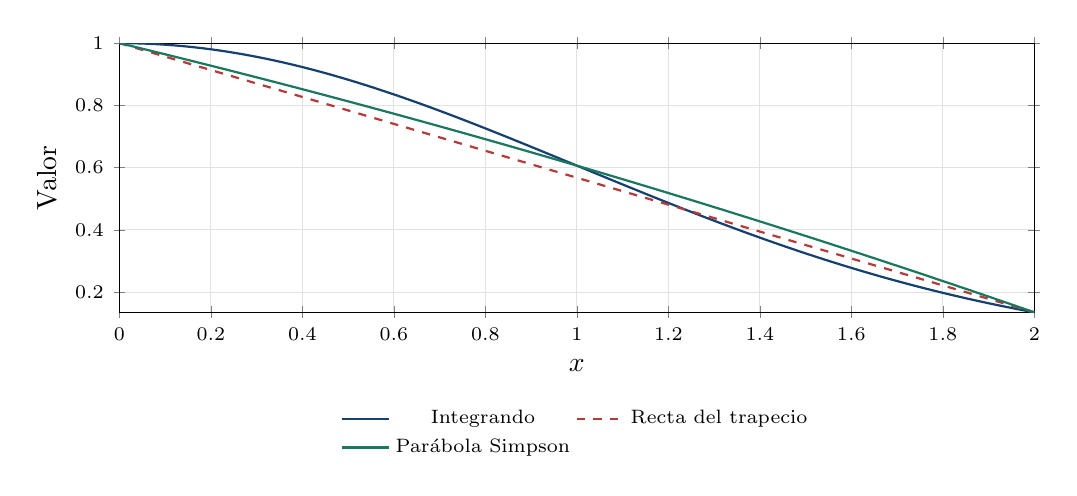
\begin{tikzpicture}\begin{axis}[base,axis lines=box,grid=major,minor tick num=0,width=13.2cm,height=5.0cm,xlabel={$x$},ylabel={Valor},legend style={at={(0.5,-0.32)},anchor=north,legend columns=2,font=\scriptsize,draw=none,fill=white}]
\addplot[thick,azul,] coordinates {(0,1) (0.02,0.99980002) (0.04,0.9992003199) (0.06,0.998201619) (0.08,0.9968051145) (0.1,0.9950124792) (0.12,0.9928258579) (0.14,0.9902478635) (0.16,0.9872815716) (0.18,0.9839305143) (0.2,0.9801986733) (0.22,0.9760904721) (0.24,0.9716107672) (0.26,0.9667648383) (0.28,0.9615583782) (0.3,0.9559974818) (0.32,0.9500886338) (0.34,0.9438386963) (0.36,0.9372548956) (0.38,0.9303448082) (0.4,0.9231163464) (0.42,0.9155777429) (0.44,0.9077375355) (0.46,0.899604551) (0.48,0.8911878885) (0.5,0.8824969026) (0.52,0.873541186) (0.54,0.864330552) (0.56,0.8548750167) (0.58,0.8451847808) (0.6,0.8352702114) (0.62,0.8251418236) (0.64,0.8148102622) (0.66,0.8042862828) (0.68,0.793580734) (0.7,0.7827045382) (0.72,0.7716686739) (0.74,0.7604841569) (0.76,0.7491620228) (0.78,0.737713309) (0.8,0.7261490371) (0.82,0.7144801955) (0.84,0.7027177229) (0.86,0.6908724913) (0.88,0.6789552903) (0.9,0.6669768109) (0.92,0.6549476305) (0.94,0.6428781982) (0.96,0.6307788205) (0.98,0.6186596475) (1,0.6065306597) (1.02,0.5944016558) (1.04,0.5822822402) (1.06,0.5701818123) (1.08,0.5581095554) (1.1,0.5460744266) (1.12,0.5340851478) (1.14,0.5221501964) (1.16,0.5102777978) (1.18,0.4984759178) (1.2,0.486752256) (1.22,0.4751142393) (1.24,0.4635690175) (1.26,0.4521234577) (1.28,0.4407841408) (1.3,0.4295573582) (1.32,0.4184491089) (1.34,0.4074650976) (1.36,0.3966107333) (1.38,0.3858911284) (1.4,0.3753110989) (1.42,0.3648751641) (1.44,0.3545875486) (1.46,0.3444521828) (1.48,0.3344727057) (1.5,0.3246524674) (1.52,0.3149945317) (1.54,0.3055016804) (1.56,0.2961764167) (1.58,0.2870209699) (1.6,0.2780373005) (1.62,0.2692271047) (1.64,0.260591821) (1.66,0.2521326351) (1.68,0.2438504869) (1.7,0.2357460766) (1.72,0.2278198714) (1.74,0.220072113) (1.76,0.2125028243) (1.78,0.205111817) (1.8,0.1978986991) (1.82,0.1908628828) (1.84,0.184003592) (1.86,0.1773198704) (1.88,0.1708105895) (1.9,0.1644744566) (1.92,0.1583100226) (1.94,0.1523156906) (1.96,0.1464897235) (1.98,0.1408302521) (2,0.1353352832)};
\addlegendentry{Integrando}
\addplot[thick,rojo,dashed] coordinates {(0,1) (0.02,0.9913533528) (0.04,0.9827067057) (0.06,0.9740600585) (0.08,0.9654134113) (0.1,0.9567667642) (0.12,0.948120117) (0.14,0.9394734698) (0.16,0.9308268227) (0.18,0.9221801755) (0.2,0.9135335283) (0.22,0.9048868812) (0.24,0.896240234) (0.26,0.8875935868) (0.28,0.8789469397) (0.3,0.8703002925) (0.32,0.8616536453) (0.34,0.8530069982) (0.36,0.844360351) (0.38,0.8357137038) (0.4,0.8270670566) (0.42,0.8184204095) (0.44,0.8097737623) (0.46,0.8011271151) (0.48,0.792480468) (0.5,0.7838338208) (0.52,0.7751871736) (0.54,0.7665405265) (0.56,0.7578938793) (0.58,0.7492472321) (0.6,0.740600585) (0.62,0.7319539378) (0.64,0.7233072906) (0.66,0.7146606435) (0.68,0.7060139963) (0.7,0.6973673491) (0.72,0.688720702) (0.74,0.6800740548) (0.76,0.6714274076) (0.78,0.6627807605) (0.8,0.6541341133) (0.82,0.6454874661) (0.84,0.636840819) (0.86,0.6281941718) (0.88,0.6195475246) (0.9,0.6109008775) (0.92,0.6022542303) (0.94,0.5936075831) (0.96,0.584960936) (0.98,0.5763142888) (1,0.5676676416) (1.02,0.5590209945) (1.04,0.5503743473) (1.06,0.5417277001) (1.08,0.5330810529) (1.1,0.5244344058) (1.12,0.5157877586) (1.14,0.5071411114) (1.16,0.4984944643) (1.18,0.4898478171) (1.2,0.4812011699) (1.22,0.4725545228) (1.24,0.4639078756) (1.26,0.4552612284) (1.28,0.4466145813) (1.3,0.4379679341) (1.32,0.4293212869) (1.34,0.4206746398) (1.36,0.4120279926) (1.38,0.4033813454) (1.4,0.3947346983) (1.42,0.3860880511) (1.44,0.3774414039) (1.46,0.3687947568) (1.48,0.3601481096) (1.5,0.3515014624) (1.52,0.3428548153) (1.54,0.3342081681) (1.56,0.3255615209) (1.58,0.3169148738) (1.6,0.3082682266) (1.62,0.2996215794) (1.64,0.2909749323) (1.66,0.2823282851) (1.68,0.2736816379) (1.7,0.2650349908) (1.72,0.2563883436) (1.74,0.2477416964) (1.76,0.2390950492) (1.78,0.2304484021) (1.8,0.2218017549) (1.82,0.2131551077) (1.84,0.2045084606) (1.86,0.1958618134) (1.88,0.1872151662) (1.9,0.1785685191) (1.92,0.1699218719) (1.94,0.1612752247) (1.96,0.1526285776) (1.98,0.1439819304) (2,0.1353352832)};
\addlegendentry{Recta del trapecio}
\addplot[thick,verde,] coordinates {(0,1) (0.02,0.9928923283) (0.04,0.9857535663) (0.06,0.9785837138) (0.08,0.9713827709) (0.1,0.9641507376) (0.12,0.9568876139) (0.14,0.9495933997) (0.16,0.9422680952) (0.18,0.9349117002) (0.2,0.9275242148) (0.22,0.920105639) (0.24,0.9126559728) (0.26,0.9051752162) (0.28,0.8976633692) (0.3,0.8901204317) (0.32,0.8825464038) (0.34,0.8749412856) (0.36,0.8673050769) (0.38,0.8596377778) (0.4,0.8519393882) (0.42,0.8442099083) (0.44,0.8364493379) (0.46,0.8286576772) (0.48,0.820834926) (0.5,0.8129810844) (0.52,0.8050961524) (0.54,0.7971801299) (0.56,0.7892330171) (0.58,0.7812548138) (0.6,0.7732455202) (0.62,0.7652051361) (0.64,0.7571336616) (0.66,0.7490310967) (0.68,0.7408974413) (0.7,0.7327326956) (0.72,0.7245368594) (0.74,0.7163099329) (0.76,0.7080519159) (0.78,0.6997628085) (0.8,0.6914426107) (0.82,0.6830913224) (0.84,0.6747089438) (0.86,0.6662954747) (0.88,0.6578509153) (0.9,0.6493752654) (0.92,0.6408685251) (0.94,0.6323306944) (0.96,0.6237617732) (0.98,0.6151617617) (1,0.6065306597) (1.02,0.5978684673) (1.04,0.5891751845) (1.06,0.5804508113) (1.08,0.5716953477) (1.1,0.5629087937) (1.12,0.5540911492) (1.14,0.5452424144) (1.16,0.5363625891) (1.18,0.5274516734) (1.2,0.5185096673) (1.22,0.5095365708) (1.24,0.5005323839) (1.26,0.4914971065) (1.28,0.4824307387) (1.3,0.4733332806) (1.32,0.464204732) (1.34,0.455045093) (1.36,0.4458543636) (1.38,0.4366325437) (1.4,0.4273796335) (1.42,0.4180956328) (1.44,0.4087805417) (1.46,0.3994343602) (1.48,0.3900570883) (1.5,0.380648726) (1.52,0.3712092733) (1.54,0.3617387301) (1.56,0.3522370965) (1.58,0.3427043726) (1.6,0.3331405582) (1.62,0.3235456534) (1.64,0.3139196581) (1.66,0.3042625725) (1.68,0.2945743964) (1.7,0.28485513) (1.72,0.2751047731) (1.74,0.2653233258) (1.76,0.2555107881) (1.78,0.24566716) (1.8,0.2357924414) (1.82,0.2258866325) (1.84,0.2159497331) (1.86,0.2059817433) (1.88,0.1959826631) (1.9,0.1859524925) (1.92,0.1758912315) (1.94,0.16579888) (1.96,0.1556754382) (1.98,0.1455209059) (2,0.1353352832)};
\addlegendentry{Parábola Simpson}
\end{axis}\end{tikzpicture}
\caption{Trapecio y Simpson integran interpolantes diferentes. La exactitud polinómica y el signo del error se deducen de los restos y núcleos, no solo de esta imagen.}\label{fig:cdf-4}\end{figure}

\section{Derivadas normales y cotas computables}
Como $\ph'=-x\ph$,
\begin{align*}
\ph''&=(x^2-1)\ph,\\
\ph'''&=(3x-x^3)\ph,\\
\ph^{(4)}&=(x^4-6x^2+3)\ph.
\end{align*}
En $[0,1]$, una cota simple es $|\ph''|\le1/\sqrt{2\pi}$ y
$|\ph^{(4)}|\le10/\sqrt{2\pi}$, aunque esta última puede afinarse. Para aproximar $\Phi(1)=1/2+\int_0^1\ph$ con Simpson compuesto,
\[
|E|\le\frac1{180n^4}\frac{10}{\sqrt{2\pi}}.
\]
La cota necesita derivadas del integrando, no de la CDF. Para integrar $\Phi$ misma, las derivadas cambian.

Con $n=2$, la aproximación explícita es
\[
\Phi(1)\approx\frac12+\frac16[\ph(0)+4\ph(1/2)+\ph(1)].
\]
Esta fórmula es un primer algoritmo desde cero. Será comparada con Gauss, Taylor, una serie positiva y un evaluador de referencia.

\section{Newton--Cotes de orden alto y pesos negativos}
Para nodos equiespaciados en $[a,b]$, integrar el interpolante produce reglas Newton--Cotes. En grado bajo son simples y útiles. En grado alto algunos pesos pueden ser negativos. Entonces una función positiva puede producir una suma negativa, y los errores de evaluación pueden amplificarse.

Si $|\Delta f_i|\le\eta$,
\[
|\Delta\mathcal Q|\le\eta\sum_i|w_i|.
\]
Para pesos positivos, $\sum|w_i|=\sum w_i=\int w$, el menor valor posible compatible con exactitud para constantes. Pesos negativos hacen mayor esa cantidad.

La solución habitual no es aumentar indefinidamente el grado equiespaciado. Se usa una regla compuesta de grado bajo, o nodos de Gauss/Chebyshev. El costo debe medirse por evaluaciones de $f$, y la precisión por una métrica apropiada a la integral.

\section{Núcleo de Peano: una prueba unificada del error}
Sea $L(f)=I(f)-\mathcal Q(f)$ un funcional lineal que anula polinomios de grado menor que $r$. Taylor con resto integral alrededor de $a$ permite escribir
\[
f(x)=p_{r-1}(x)+\int_a^b
\frac{(x-t)_+^{r-1}}{(r-1)!}f^{(r)}(t)\dd t,
\]
donde $s_+=\max(s,0)$. Aplicando $L$ y usando $L(p)=0$,
\[
L(f)=\int_a^b K_r(t)f^{(r)}(t)\dd t,\qquad
K_r(t)=L\left(\frac{(x-t)_+^{r-1}}{(r-1)!}\right).
\]
Por tanto $|L(f)|\le\norm{f^{(r)}}_\infty\int|K_r|$. Si $K_r$ tiene signo fijo y $f^{(r)}$ es continua, existe $\xi$ con
$L(f)=f^{(r)}(\xi)\int K_r$.

Este teorema explica por qué muchas fórmulas de error tienen una sola derivada en un punto desconocido. También muestra cuándo esa forma es inválida: si el núcleo cambia de signo, una media ponderada con pesos negativos no se reduce al mismo argumento.

\section{Euler--Maclaurin y correcciones de extremos}
Para $f$ suficientemente suave, el trapecio compuesto tiene expansión
\[
T_n-I=\frac{\Delta^2}{12}[f'(b)-f'(a)]
-\frac{\Delta^4}{720}[f'''(b)-f'''(a)]+\cdots.
\]
Los coeficientes se relacionan con Bernoulli: $B_2=1/6$, $B_4=-1/30$. Una deducción comienza integrando por partes contra una función periódica lineal por tramos que representa el error de una malla; integrar de nuevo produce polinomios de Bernoulli.

Para comprobar el primer término, $f(x)=x^2$ en $[0,1]$ da
$T_n-I=\Delta^2/6$, pues $f'(1)-f'(0)=2$. No hay términos posteriores porque las derivadas altas son cero.

Una regla corregida es
\[
T_n^{\rm corr}=T_n-\frac{\Delta^2}{12}[f'(b)-f'(a)].
\]
Mejora el orden si las derivadas existen y pueden calcularse. Para una densidad gamma singular en cero, las hipótesis pueden fallar: aplicar ciegamente una expansión de funciones suaves puede dar una falsa confianza.

\section{Richardson y la eliminación algebraica del error}
Supongamos $A(h)=I+ch^p+O(h^{p+q})$ y $A(h/2)=I+c(h/2)^p+O(h^{p+q})$. Eliminando $c$,
\[
R(h)=\frac{2^pA(h/2)-A(h)}{2^p-1}
=I+O(h^{p+q}).
\]
No se necesita conocer $c$, pero sí el exponente principal $p$. Si el integrando es singular o el régimen asintótico no ha comenzado, el orden observado puede ser distinto.

La diferencia $A(h/2)-A(h)\approx-(1-2^{-p})ch^p$ proporciona una estimación práctica del error fino,
\[
I-A(h/2)\approx\frac{A(h/2)-A(h)}{2^p-1}.
\]
No es automáticamente una cota certificada. Puede fallar si dos errores se cancelan o si las reglas no detectan una característica estrecha del integrando.






\begin{figure}[htbp]\centering
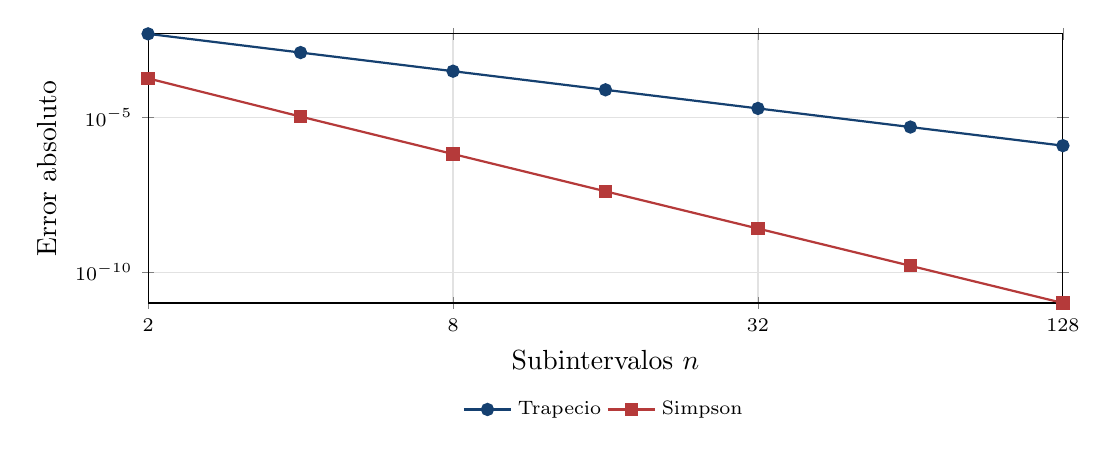
\begin{tikzpicture}\begin{axis}[base,axis lines=box,grid=major,minor tick num=0,width=13.2cm,height=5.0cm,xmode=log,ymode=log,xlabel={Subintervalos $n$},ylabel={Error absoluto},xtick={2,8,32,128},xticklabels={2,8,32,128},legend style={at={(0.5,-0.32)},anchor=north,legend columns=2,font=\scriptsize,draw=none,fill=white}]
\addplot[thick,azul,mark=*] coordinates {(2,0.005083831456) (4,0.001262901523) (8,0.0003152303278) (16,7.877677081e-05) (32,1.969226902e-05) (64,4.922947056e-06) (128,1.230729252e-06)};
\addlegendentry{Trapecio}
\addplot[thick,rojo,mark=square*] coordinates {(2,0.0001843059278) (4,1.074178811e-05) (8,6.600705501e-07) (16,4.108153578e-08) (32,2.564908674e-09) (64,1.602648569e-10) (128,1.001593253e-11)};
\addlegendentry{Simpson}
\end{axis}\end{tikzpicture}
\caption{Convergencia observada para $\int_0^1\varphi$. Las pendientes corresponden a órdenes dos y cuatro antes de que domine el redondeo. Esta gráfica es una prueba del caso, no una cota universal.}\label{fig:cdf-5}\end{figure}

\section{Romberg como tabla triangular}
Definamos $R_{k,0}=T_{2^k}$ y
\[
R_{k,j}=R_{k,j-1}+
\frac{R_{k,j-1}-R_{k-1,j-1}}{4^j-1},
\qquad j=1,\ldots,k.
\]
Cada columna elimina otro término par de Euler--Maclaurin. La tabla no puede calcular una entrada antes de conocer las dos de la columna anterior. La actualización trapezoidal reutiliza valores:
\[
T_{2n}=\frac12T_n+\frac{\Delta}2
\sum_{i=0}^{n-1}f(a+(i+1/2)\Delta).
\]
El costo adicional es $n$ evaluaciones.

Romberg funciona bien para funciones suaves en intervalos compactos. Si $f(x)=\sqrt x$ en $[0,1]$, las derivadas en cero no satisfacen las hipótesis necesarias para una expansión solo en potencias pares. Un cambio $x=t^2$ produce un integrando polinómico y transforma el problema antes de extrapolar.

\section{Adaptación por bisección y presupuesto local}
Calculemos Simpson $S$ en $[a,b]$ y la suma $S_2$ de dos Simpson en mitades. Si el error principal tiene orden cuatro respecto de la malla,
\[
I-S_2\approx\frac{S_2-S}{15},\qquad
S_{\rm corr}=S_2+\frac{S_2-S}{15}.
\]
Un procedimiento divide el intervalo si $|S_2-S|/15$ excede su tolerancia asignada. Al partirlo, reparte el presupuesto entre hijos y suma los resultados.

Las evaluaciones en extremos y punto medio se reutilizan. Se necesitan límites de profundidad y detección de $m=(a+b)/2$ igual a un extremo por redondeo. Si la función no es finita en un extremo, Simpson cerrado no se aplica directamente.

El estimador se basa en un modelo de error. No puede garantizar descubrir una aguja estrecha que ningún nodo toca. Una certificación real exige hipótesis sobre derivadas o un esquema de intervalos que encierre el integrando.

\section{Gauss--Kronrod y el significado de una pareja embebida}
Una regla Gauss de $n$ nodos puede extenderse, cuando la familia admite una extensión apropiada, con nodos adicionales que conservan los antiguos. El esquema Kronrod clásico tiene $2n+1$ nodos y busca mayor exactitud. Ambas estimaciones usan valores compartidos:
\[
G_n(f)=\sum_iw_i^{G}f(x_i),\qquad
K_{2n+1}(f)=\sum_iw_i^{K}f(x_i).
\]
La diferencia $|K-G|$ es un indicador de error, no la definición del error exacto. Los pesos Gauss y Kronrod en los nodos comunes son distintos.

La adaptación moderna suele usar una cola de intervalos ordenada por el error estimado. Se divide primero el que más contribuye al total. Un criterio frecuente es
$E_{\rm est}\le\max(\tau_{\rm abs},\tau_{\rm rel}|I_{\rm est}|)$.
Si la integral es casi cero por cancelación, la tolerancia absoluta evita un requisito relativo imposible de interpretar.

\section{Una integral oscilatoria y por qué no basta densificar}
Para $I(\omega)=\int_a^b g(x)e^{i\omega x}\dd x$, $|\omega|$ grande produce cancelación. Si $\omega\ne0$ y $g$ es derivable,
\[
I(\omega)=\left[\frac{g(x)e^{i\omega x}}{i\omega}\right]_a^b
-\frac1{i\omega}\int_a^b g'(x)e^{i\omega x}\dd x.
\]
El resultado puede tener tamaño $1/|\omega|$ aunque $|g|$ sea de orden uno. Filon interpola la amplitud y integra exactamente el factor oscilatorio. Levin busca $p$ tal que $p'+i\omega p=g$ y usa $[pe^{i\omega x}]_a^b$.

Estas ideas reaparecen al invertir funciones características para obtener CDF. Un problema no positivo requiere un análisis de cancelación distinto del de una densidad integrada directamente.

\section{Transformaciones doble exponenciales}
Para $x\in[-1,1]$ usemos
\[
x=\tanh\left(\frac\pi2\sinh t\right),\quad
\psi'(t)=\frac{(\pi/2)\cosh t}
{\cosh^2((\pi/2)\sinh t)}.
\]
Entonces $\int_{-1}^1f(x)\dd x=\int_\R f(\psi(t))\psi'(t)\dd t$. La distancia de $\psi(t)$ a un extremo decrece aproximadamente como $\exp(-c e^{|t|})$. Incluso singularidades algebraicas integrables quedan multiplicadas por un jacobiano que cae muy rápidamente.

La regla tanh--sinh es
\[
I\approx h\sum_{k=-N}^N f(\psi(kh))\psi'(kh).
\]
Hay error por truncar $|k|>N$ y error por usar paso $h$. Reducir $h$ sin ampliar $Nh$ no elimina el primero. En computadora $\psi(t)$ puede redondear exactamente a $\pm1$: conviene evaluar distancias a extremos de manera estable cuando $f$ diverge allí.

El método Takahasi--Mori no vuelve universalmente óptima toda integral. Analiticidad, singularidades complejas y escala gobiernan su desempeño. Para CDF gamma/beta difíciles es una referencia independiente útil frente a series y fracciones continuas.







\begin{figure}[htbp]\centering
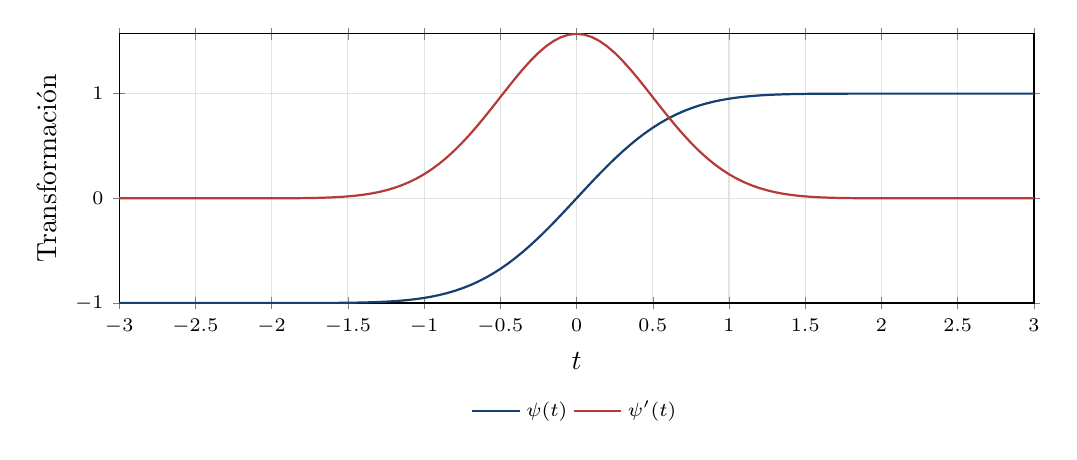
\begin{tikzpicture}\begin{axis}[base,axis lines=box,grid=major,minor tick num=0,width=13.2cm,height=5.0cm,xlabel={$t$},ylabel={Transformación},legend style={at={(0.5,-0.32)},anchor=north,legend columns=2,font=\scriptsize,draw=none,fill=white}]
\addplot[thick,azul,] coordinates {(-3,-1) (-2.95,-1) (-2.9,-1) (-2.85,-1) (-2.8,-1) (-2.75,-1) (-2.7,-0.9999999998) (-2.65,-0.9999999995) (-2.6,-0.9999999985) (-2.55,-0.9999999959) (-2.5,-0.9999999889) (-2.45,-0.9999999715) (-2.4,-0.9999999303) (-2.35,-0.9999998367) (-2.3,-0.9999996326) (-2.25,-0.9999992047) (-2.2,-0.9999983409) (-2.15,-0.999996658) (-2.1,-0.9999934882) (-2.05,-0.9999877064) (-2,-0.9999774772) (-1.95,-0.9999598957) (-1.9,-0.9999304959) (-1.85,-0.9998825978) (-1.8,-0.999806467) (-1.75,-0.999688264) (-1.7,-0.9995087691) (-1.65,-0.9992418774) (-1.6,-0.9988528715) (-1.55,-0.9982964938) (-1.5,-0.9975148565) (-1.45,-0.9964352425) (-1.4,-0.9949678687) (-1.35,-0.9930036963) (-1.3,-0.9904123929) (-1.25,-0.9870405605) (-1.2,-0.9827103622) (-1.15,-0.9772186895) (-1.1,-0.9703370259) (-1.05,-0.9618121672) (-1,-0.9513679641) (-0.95,-0.9387082456) (-0.9,-0.9235210705) (-0.85,-0.9054844219) (-0.8,-0.8842734197) (-0.75,-0.8595690587) (-0.7,-0.8310683974) (-0.65,-0.7984960186) (-0.6,-0.7616164592) (-0.55,-0.7202471775) (-0.5,-0.6742714922) (-0.45,-0.6236508075) (-0.4,-0.5684353519) (-0.35,-0.5087726131) (-0.3,-0.4449126727) (-0.25,-0.3772097382) (-0.2,-0.3061193439) (-0.15,-0.2321909398) (-0.1,-0.1560558911) (-0.05,-0.07841125066) (0,0) (0.05,0.07841125066) (0.1,0.1560558911) (0.15,0.2321909398) (0.2,0.3061193439) (0.25,0.3772097382) (0.3,0.4449126727) (0.35,0.5087726131) (0.4,0.5684353519) (0.45,0.6236508075) (0.5,0.6742714922) (0.55,0.7202471775) (0.6,0.7616164592) (0.65,0.7984960186) (0.7,0.8310683974) (0.75,0.8595690587) (0.8,0.8842734197) (0.85,0.9054844219) (0.9,0.9235210705) (0.95,0.9387082456) (1,0.9513679641) (1.05,0.9618121672) (1.1,0.9703370259) (1.15,0.9772186895) (1.2,0.9827103622) (1.25,0.9870405605) (1.3,0.9904123929) (1.35,0.9930036963) (1.4,0.9949678687) (1.45,0.9964352425) (1.5,0.9975148565) (1.55,0.9982964938) (1.6,0.9988528715) (1.65,0.9992418774) (1.7,0.9995087691) (1.75,0.999688264) (1.8,0.999806467) (1.85,0.9998825978) (1.9,0.9999304959) (1.95,0.9999598957) (2,0.9999774772) (2.05,0.9999877064) (2.1,0.9999934882) (2.15,0.999996658) (2.2,0.9999983409) (2.25,0.9999992047) (2.3,0.9999996326) (2.35,0.9999998367) (2.4,0.9999999303) (2.45,0.9999999715) (2.5,0.9999999889) (2.55,0.9999999959) (2.6,0.9999999985) (2.65,0.9999999995) (2.7,0.9999999998) (2.75,1) (2.8,1) (2.85,1) (2.9,1) (2.95,1) (3,1)};
\addlegendentry{$\psi(t)$}
\addplot[thick,rojo,] coordinates {(-3,1.358178427e-12) (-2.95,6.044445691e-12) (-2.9,2.496122113e-11) (-2.85,9.600197989e-11) (-2.8,3.45078361e-10) (-2.75,1.163116581e-09) (-2.7,3.687837968e-09) (-2.65,1.103245796e-08) (-2.6,3.122988656e-08) (-2.55,8.387878917e-08) (-2.5,2.143120456e-07) (-2.45,5.221901936e-07) (-2.4,1.216248232e-06) (-2.35,2.713951162e-06) (-2.3,5.814290631e-06) (-2.25,1.198370136e-05) (-2.2,2.380825833e-05) (-2.15,4.567829698e-05) (-2.1,8.478194367e-05) (-2.05,0.0001524887445) (-2,0.0002662005138) (-1.95,0.0004517310866) (-1.9,0.0007462484304) (-1.85,0.001201771867) (-1.8,0.001889166235) (-1.75,0.002902517748) (-1.7,0.00436371822) (-1.65,0.006427030823) (-1.6,0.009283366129) (-1.55,0.01316396512) (-1.5,0.01834316699) (-1.45,0.02513993276) (-1.4,0.03391779868) (-1.35,0.04508294214) (-1.3,0.05908005611) (-1.25,0.07638574357) (-1.2,0.0974991644) (-1.15,0.1229296979) (-1.1,0.1531814334) (-1.05,0.1887343783) (-1,0.2300223945) (-0.95,0.2774080434) (-0.9,0.3311547553) (-0.85,0.3913970387) (-0.8,0.4581098035) (-0.75,0.5310782754) (-0.7,0.6098703962) (-0.65,0.6938139832) (-0.6,0.7819812122) (-0.55,0.8731831037) (-0.5,0.9659765794) (-0.45,1.058686231) (-0.4,1.14944218) (-0.35,1.236234303) (-0.3,1.316981703) (-0.25,1.389614759) (-0.2,1.452165494) (-0.15,1.502860677) (-0.1,1.540211129) (-0.05,1.563090391) (0,1.570796327) (0.05,1.563090391) (0.1,1.540211129) (0.15,1.502860677) (0.2,1.452165494) (0.25,1.389614759) (0.3,1.316981703) (0.35,1.236234303) (0.4,1.14944218) (0.45,1.058686231) (0.5,0.9659765794) (0.55,0.8731831037) (0.6,0.7819812122) (0.65,0.6938139832) (0.7,0.6098703962) (0.75,0.5310782754) (0.8,0.4581098035) (0.85,0.3913970387) (0.9,0.3311547553) (0.95,0.2774080434) (1,0.2300223945) (1.05,0.1887343783) (1.1,0.1531814334) (1.15,0.1229296979) (1.2,0.0974991644) (1.25,0.07638574357) (1.3,0.05908005611) (1.35,0.04508294214) (1.4,0.03391779868) (1.45,0.02513993276) (1.5,0.01834316699) (1.55,0.01316396512) (1.6,0.009283366129) (1.65,0.006427030823) (1.7,0.00436371822) (1.75,0.002902517748) (1.8,0.001889166235) (1.85,0.001201771867) (1.9,0.0007462484304) (1.95,0.0004517310866) (2,0.0002662005138) (2.05,0.0001524887445) (2.1,8.478194367e-05) (2.15,4.567829698e-05) (2.2,2.380825833e-05) (2.25,1.198370136e-05) (2.3,5.814290631e-06) (2.35,2.713951162e-06) (2.4,1.216248232e-06) (2.45,5.221901936e-07) (2.5,2.143120456e-07) (2.55,8.387878917e-08) (2.6,3.122988656e-08) (2.65,1.103245796e-08) (2.7,3.687837968e-09) (2.75,1.163116581e-09) (2.8,3.45078361e-10) (2.85,9.600197989e-11) (2.9,2.496122113e-11) (2.95,6.044445691e-12) (3,1.358178427e-12)};
\addlegendentry{$\psi'(t)$}
\end{axis}\end{tikzpicture}
\caption{Tanh--sinh lleva la recta a un intervalo finito. El jacobiano concentra evaluaciones útiles y cae doble exponencialmente en los extremos.}\label{fig:cdf-6}\end{figure}

\parte{IV. Ortogonalidad: de funciones a vectores y matrices}
\section{Producto interior ponderado}
Sea $w(x)>0$ casi en todas partes en un intervalo y supongamos que los momentos necesarios son finitos. Definimos
\[
\langle f,g\rangle_w=\int_a^b f(x)g(x)w(x)\dd x,\qquad
\norm f_w^2=\langle f,f\rangle_w.
\]
Es bilineal, simétrico y positivo para funciones reales, identificando las que coinciden casi en todas partes. En polinomios, $\norm p_w=0$ implica $p=0$, porque un polinomio no nulo no se anula en un conjunto de medida positiva.

Cauchy--Schwarz se deduce de $0\le\norm{f-tg}_w^2$ para todo $t$. El discriminante de esa cuadrática no puede ser positivo:
\[
|\langle f,g\rangle_w|^2\le\norm f_w^2\norm g_w^2.
\]
De allí la desigualdad triangular. Ortogonalidad significa producto interior cero; no implica que las gráficas no se crucen.

Una proyección sobre una base ortonormal $q_0,\ldots,q_m$ es
$p=\sum_{k=0}^m\langle f,q_k\rangle q_k$. El resto es ortogonal al subespacio y
\[
\norm{f-p}^2=\norm f^2-\sum_{k=0}^m|\langle f,q_k\rangle|^2.
\]
Es el análogo funcional de proyectar un vector sobre columnas ortonormales.

\section{Gram--Schmidt con monomios}
Partimos de $1,x,x^2,\ldots$. Definamos $p_0=1$ y, para polinomios mónicos,
\[
p_n(x)=x^n-\sum_{j=0}^{n-1}
\frac{\langle x^n,p_j\rangle_w}{\langle p_j,p_j\rangle_w}p_j(x).
\]
El coeficiente líder sigue siendo uno; tomar producto con $p_i$ elimina exactamente su componente. La existencia de momentos hasta grado $2n$ permite todos los cálculos.

Con peso uno en $[-1,1]$, $\langle1,1\rangle=2$ y $\langle x,1\rangle=0$, de modo que $p_1=x$. Para grado dos,
\[
p_2=x^2-\frac{\int_{-1}^1x^2\dd x}{2}=x^2-\frac13.
\]
Para grado tres, la simetría elimina productos con grados pares:
\[
p_3=x^3-\frac{\int x^4}{\int x^2}x=x^3-\frac35x.
\]
Sus ceros darán los nodos de Gauss de dos y tres puntos.

Gram--Schmidt es una deducción conceptual útil. Con muchos grados, los momentos monomiales pueden producir matrices mal condicionadas. Las recurrencias ortogonales permiten construir la misma familia de manera más eficaz.

\section{Matriz de momentos y positividad}
Con $v(x)=(1,x,\ldots,x^m)\T$,
\[
H_m=\int_a^b v(x)v(x)\T w(x)\dd x,\qquad
(H_m)_{ij}=\mu_{i+j}.
\]
Para un vector $c\ne0$,
\[
c\T H_mc=\int_a^b(c\T v(x))^2w(x)\dd x>0.
\]
Por tanto $H_m$ es definida positiva. Es una matriz Hankel porque sus entradas dependen de la suma de índices.

Para peso uno en $[0,1]$,
\[
H_m=\left(\frac1{i+j+1}\right)_{i,j=0}^m.
\]
Esta es la matriz de Hilbert. Su positividad exacta no implica buen condicionamiento numérico; al subir el grado puede acercarse mucho a singular en precisión finita. Resolver momentos sin escalado no es la vía recomendada para reglas de gran tamaño.

Cholesky de $H$ conecta ortogonalización con matrices triangulares. Si $H=LL\T$ y $q=L^{-1}v$, entonces $\int qq\T w=I$. La multiplicación por $x$ en esta base produce la matriz de Jacobi.

\section{Recurrencia de tres términos, demostrada}
Sea $p_n$ mónico y $h_n=\langle p_n,p_n\rangle_w>0$. Expandimos $xp_n$ en la base ortogonal hasta grado $n+1$. El coeficiente de $p_{n+1}$ es uno. Para $j\le n-2$,
\[
\langle xp_n,p_j\rangle=\langle p_n,xp_j\rangle=0,
\]
pues $xp_j$ tiene grado a lo sumo $n-1$. Solo quedan dos términos:
\[
p_{n+1}(x)=(x-\alpha_n)p_n(x)-\beta_np_{n-1}(x),
\]
\[
\alpha_n=\frac{\langle xp_n,p_n\rangle}{h_n},\qquad
\beta_n=\frac{h_n}{h_{n-1}}>0\quad(n\ge1).
\]
Para el último coeficiente, $\langle xp_n,p_{n-1}\rangle=
\langle p_n,xp_{n-1}\rangle=h_n$, porque $xp_{n-1}=p_n+$ términos menores.

Con $q_n=p_n/\sqrt{h_n}$ y $b_n=\sqrt{\beta_n}$,
\[
xq_n=b_{n+1}q_{n+1}+\alpha_nq_n+b_nq_{n-1}.
\]
Es una recurrencia simétrica. Los coeficientes $b_n$ positivos sostienen tanto la teoría de ceros como la interpretación espectral.

\section{Por qué los ceros son reales, simples e interiores}
Sea $p_n$ ortogonal a todos los grados menores. Supongamos que tiene $k<n$ cambios de signo en el interior, en $r_1,\ldots,r_k$. Formamos $s(x)=\prod_{j=1}^k(x-r_j)$. El producto $p_ns$ no cambia de signo dentro salvo ceros que no cambian signo; además no es idénticamente cero. Por tanto su integral contra un peso positivo no es cero.

Pero $\deg s=k<n$, lo que contradice $\langle p_n,s\rangle=0$. Así, hay al menos $n$ cambios de signo interiores. Un polinomio de grado $n$ solo tiene $n$ raíces contando multiplicidades: todos sus ceros son reales, distintos e interiores.

La prueba exige que el peso tenga soporte suficientemente amplio; para una medida con solo un número finito de átomos no se puede construir indefinidamente una familia positiva. En distribuciones continuas clásicas la condición se cumple.

El entrelazamiento de ceros de grados vecinos se deduce de la recurrencia y $\beta_n>0$, o de la teoría de matrices simétricas tridiagonales. Permite aislar raíces sin iniciar Newton desde una posición arbitraria.

\section{Legendre y la fórmula de Rodrigues}
Los polinomios de Legendre normalizados por $P_n(1)=1$ se construyen mediante
\[
P_n(x)=\frac1{2^n n!}\frac{\dd^n}{\dd x^n}(x^2-1)^n.
\]
Para cualquier $q$ de grado menor que $n$, integrar por partes $n$ veces da
\[
\int_{-1}^1P_n(x)q(x)\dd x
=\frac{(-1)^n}{2^n n!}\int_{-1}^1(x^2-1)^nq^{(n)}(x)\dd x=0.
\]
Todos los términos de borde desaparecen porque $(x^2-1)^n$ y sus primeras $n-1$ derivadas se anulan en ambos extremos.

Los primeros son
\[
P_0=1,\ P_1=x,\ P_2=\frac{3x^2-1}2,\ 
P_3=\frac{5x^3-3x}2,\ 
P_4=\frac{35x^4-30x^2+3}8.
\]
Satisfacen
\[
(n+1)P_{n+1}=(2n+1)xP_n-nP_{n-1},\qquad
\int_{-1}^1P_n^2=\frac2{2n+1}.
\]
La norma puede deducirse integrando Rodrigues y comparando el coeficiente líder. La normalización mónico/estándar cambia coeficientes, pero no ceros.






\begin{figure}[htbp]\centering
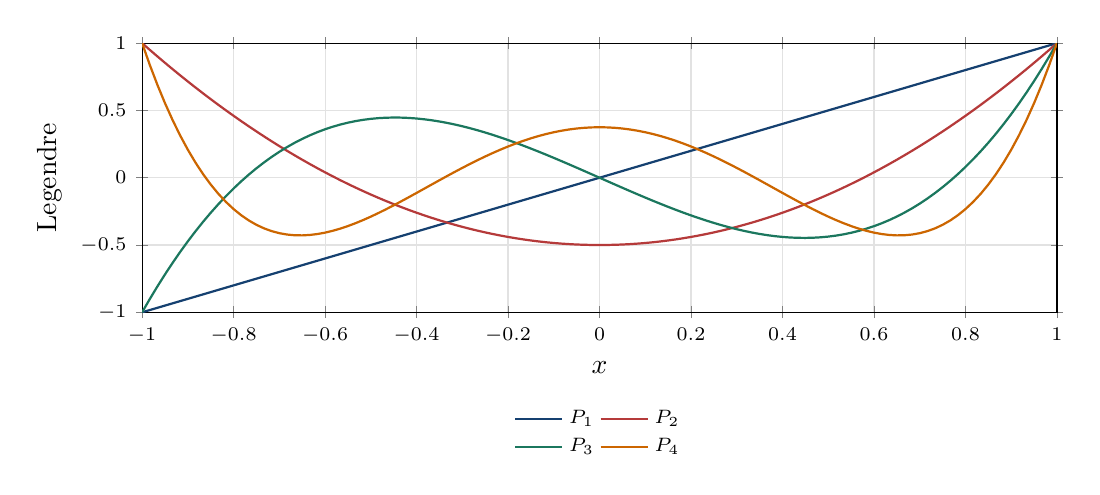
\begin{tikzpicture}\begin{axis}[base,axis lines=box,grid=major,minor tick num=0,width=13.2cm,height=5.0cm,xlabel={$x$},ylabel={Legendre},legend style={at={(0.5,-0.32)},anchor=north,legend columns=2,font=\scriptsize,draw=none,fill=white}]
\addplot[thick,azul,] coordinates {(-1,-1) (-0.9833333333,-0.9833333333) (-0.9666666667,-0.9666666667) (-0.95,-0.95) (-0.9333333333,-0.9333333333) (-0.9166666667,-0.9166666667) (-0.9,-0.9) (-0.8833333333,-0.8833333333) (-0.8666666667,-0.8666666667) (-0.85,-0.85) (-0.8333333333,-0.8333333333) (-0.8166666667,-0.8166666667) (-0.8,-0.8) (-0.7833333333,-0.7833333333) (-0.7666666667,-0.7666666667) (-0.75,-0.75) (-0.7333333333,-0.7333333333) (-0.7166666667,-0.7166666667) (-0.7,-0.7) (-0.6833333333,-0.6833333333) (-0.6666666667,-0.6666666667) (-0.65,-0.65) (-0.6333333333,-0.6333333333) (-0.6166666667,-0.6166666667) (-0.6,-0.6) (-0.5833333333,-0.5833333333) (-0.5666666667,-0.5666666667) (-0.55,-0.55) (-0.5333333333,-0.5333333333) (-0.5166666667,-0.5166666667) (-0.5,-0.5) (-0.4833333333,-0.4833333333) (-0.4666666667,-0.4666666667) (-0.45,-0.45) (-0.4333333333,-0.4333333333) (-0.4166666667,-0.4166666667) (-0.4,-0.4) (-0.3833333333,-0.3833333333) (-0.3666666667,-0.3666666667) (-0.35,-0.35) (-0.3333333333,-0.3333333333) (-0.3166666667,-0.3166666667) (-0.3,-0.3) (-0.2833333333,-0.2833333333) (-0.2666666667,-0.2666666667) (-0.25,-0.25) (-0.2333333333,-0.2333333333) (-0.2166666667,-0.2166666667) (-0.2,-0.2) (-0.1833333333,-0.1833333333) (-0.1666666667,-0.1666666667) (-0.15,-0.15) (-0.1333333333,-0.1333333333) (-0.1166666667,-0.1166666667) (-0.1,-0.1) (-0.08333333333,-0.08333333333) (-0.06666666667,-0.06666666667) (-0.05,-0.05) (-0.03333333333,-0.03333333333) (-0.01666666667,-0.01666666667) (0,0) (0.01666666667,0.01666666667) (0.03333333333,0.03333333333) (0.05,0.05) (0.06666666667,0.06666666667) (0.08333333333,0.08333333333) (0.1,0.1) (0.1166666667,0.1166666667) (0.1333333333,0.1333333333) (0.15,0.15) (0.1666666667,0.1666666667) (0.1833333333,0.1833333333) (0.2,0.2) (0.2166666667,0.2166666667) (0.2333333333,0.2333333333) (0.25,0.25) (0.2666666667,0.2666666667) (0.2833333333,0.2833333333) (0.3,0.3) (0.3166666667,0.3166666667) (0.3333333333,0.3333333333) (0.35,0.35) (0.3666666667,0.3666666667) (0.3833333333,0.3833333333) (0.4,0.4) (0.4166666667,0.4166666667) (0.4333333333,0.4333333333) (0.45,0.45) (0.4666666667,0.4666666667) (0.4833333333,0.4833333333) (0.5,0.5) (0.5166666667,0.5166666667) (0.5333333333,0.5333333333) (0.55,0.55) (0.5666666667,0.5666666667) (0.5833333333,0.5833333333) (0.6,0.6) (0.6166666667,0.6166666667) (0.6333333333,0.6333333333) (0.65,0.65) (0.6666666667,0.6666666667) (0.6833333333,0.6833333333) (0.7,0.7) (0.7166666667,0.7166666667) (0.7333333333,0.7333333333) (0.75,0.75) (0.7666666667,0.7666666667) (0.7833333333,0.7833333333) (0.8,0.8) (0.8166666667,0.8166666667) (0.8333333333,0.8333333333) (0.85,0.85) (0.8666666667,0.8666666667) (0.8833333333,0.8833333333) (0.9,0.9) (0.9166666667,0.9166666667) (0.9333333333,0.9333333333) (0.95,0.95) (0.9666666667,0.9666666667) (0.9833333333,0.9833333333) (1,1)};
\addlegendentry{$P_1$}
\addplot[thick,rojo,] coordinates {(-1,1) (-0.9833333333,0.9504166667) (-0.9666666667,0.9016666667) (-0.95,0.85375) (-0.9333333333,0.8066666667) (-0.9166666667,0.7604166667) (-0.9,0.715) (-0.8833333333,0.6704166667) (-0.8666666667,0.6266666667) (-0.85,0.58375) (-0.8333333333,0.5416666667) (-0.8166666667,0.5004166667) (-0.8,0.46) (-0.7833333333,0.4204166667) (-0.7666666667,0.3816666667) (-0.75,0.34375) (-0.7333333333,0.3066666667) (-0.7166666667,0.2704166667) (-0.7,0.235) (-0.6833333333,0.2004166667) (-0.6666666667,0.1666666667) (-0.65,0.13375) (-0.6333333333,0.1016666667) (-0.6166666667,0.07041666667) (-0.6,0.04) (-0.5833333333,0.01041666667) (-0.5666666667,-0.01833333333) (-0.55,-0.04625) (-0.5333333333,-0.07333333333) (-0.5166666667,-0.09958333333) (-0.5,-0.125) (-0.4833333333,-0.1495833333) (-0.4666666667,-0.1733333333) (-0.45,-0.19625) (-0.4333333333,-0.2183333333) (-0.4166666667,-0.2395833333) (-0.4,-0.26) (-0.3833333333,-0.2795833333) (-0.3666666667,-0.2983333333) (-0.35,-0.31625) (-0.3333333333,-0.3333333333) (-0.3166666667,-0.3495833333) (-0.3,-0.365) (-0.2833333333,-0.3795833333) (-0.2666666667,-0.3933333333) (-0.25,-0.40625) (-0.2333333333,-0.4183333333) (-0.2166666667,-0.4295833333) (-0.2,-0.44) (-0.1833333333,-0.4495833333) (-0.1666666667,-0.4583333333) (-0.15,-0.46625) (-0.1333333333,-0.4733333333) (-0.1166666667,-0.4795833333) (-0.1,-0.485) (-0.08333333333,-0.4895833333) (-0.06666666667,-0.4933333333) (-0.05,-0.49625) (-0.03333333333,-0.4983333333) (-0.01666666667,-0.4995833333) (0,-0.5) (0.01666666667,-0.4995833333) (0.03333333333,-0.4983333333) (0.05,-0.49625) (0.06666666667,-0.4933333333) (0.08333333333,-0.4895833333) (0.1,-0.485) (0.1166666667,-0.4795833333) (0.1333333333,-0.4733333333) (0.15,-0.46625) (0.1666666667,-0.4583333333) (0.1833333333,-0.4495833333) (0.2,-0.44) (0.2166666667,-0.4295833333) (0.2333333333,-0.4183333333) (0.25,-0.40625) (0.2666666667,-0.3933333333) (0.2833333333,-0.3795833333) (0.3,-0.365) (0.3166666667,-0.3495833333) (0.3333333333,-0.3333333333) (0.35,-0.31625) (0.3666666667,-0.2983333333) (0.3833333333,-0.2795833333) (0.4,-0.26) (0.4166666667,-0.2395833333) (0.4333333333,-0.2183333333) (0.45,-0.19625) (0.4666666667,-0.1733333333) (0.4833333333,-0.1495833333) (0.5,-0.125) (0.5166666667,-0.09958333333) (0.5333333333,-0.07333333333) (0.55,-0.04625) (0.5666666667,-0.01833333333) (0.5833333333,0.01041666667) (0.6,0.04) (0.6166666667,0.07041666667) (0.6333333333,0.1016666667) (0.65,0.13375) (0.6666666667,0.1666666667) (0.6833333333,0.2004166667) (0.7,0.235) (0.7166666667,0.2704166667) (0.7333333333,0.3066666667) (0.75,0.34375) (0.7666666667,0.3816666667) (0.7833333333,0.4204166667) (0.8,0.46) (0.8166666667,0.5004166667) (0.8333333333,0.5416666667) (0.85,0.58375) (0.8666666667,0.6266666667) (0.8833333333,0.6704166667) (0.9,0.715) (0.9166666667,0.7604166667) (0.9333333333,0.8066666667) (0.95,0.85375) (0.9666666667,0.9016666667) (0.9833333333,0.9504166667) (1,1)};
\addlegendentry{$P_2$}
\addplot[thick,verde,] coordinates {(-1,-1) (-0.9833333333,-0.9020717593) (-0.9666666667,-0.8082407407) (-0.95,-0.7184375) (-0.9333333333,-0.6325925926) (-0.9166666667,-0.5506365741) (-0.9,-0.4725) (-0.8833333333,-0.3981134259) (-0.8666666667,-0.3274074074) (-0.85,-0.2603125) (-0.8333333333,-0.1967592593) (-0.8166666667,-0.1366782407) (-0.8,-0.08) (-0.7833333333,-0.02665509259) (-0.7666666667,0.02342592593) (-0.75,0.0703125) (-0.7333333333,0.1140740741) (-0.7166666667,0.1547800926) (-0.7,0.1925) (-0.6833333333,0.2273032407) (-0.6666666667,0.2592592593) (-0.65,0.2884375) (-0.6333333333,0.3149074074) (-0.6166666667,0.3387384259) (-0.6,0.36) (-0.5833333333,0.3787615741) (-0.5666666667,0.3950925926) (-0.55,0.4090625) (-0.5333333333,0.4207407407) (-0.5166666667,0.4301967593) (-0.5,0.4375) (-0.4833333333,0.4427199074) (-0.4666666667,0.4459259259) (-0.45,0.4471875) (-0.4333333333,0.4465740741) (-0.4166666667,0.4441550926) (-0.4,0.44) (-0.3833333333,0.4341782407) (-0.3666666667,0.4267592593) (-0.35,0.4178125) (-0.3333333333,0.4074074074) (-0.3166666667,0.3956134259) (-0.3,0.3825) (-0.2833333333,0.3681365741) (-0.2666666667,0.3525925926) (-0.25,0.3359375) (-0.2333333333,0.3182407407) (-0.2166666667,0.2995717593) (-0.2,0.28) (-0.1833333333,0.2595949074) (-0.1666666667,0.2384259259) (-0.15,0.2165625) (-0.1333333333,0.1940740741) (-0.1166666667,0.1710300926) (-0.1,0.1475) (-0.08333333333,0.1235532407) (-0.06666666667,0.09925925926) (-0.05,0.0746875) (-0.03333333333,0.04990740741) (-0.01666666667,0.02498842593) (0,0) (0.01666666667,-0.02498842593) (0.03333333333,-0.04990740741) (0.05,-0.0746875) (0.06666666667,-0.09925925926) (0.08333333333,-0.1235532407) (0.1,-0.1475) (0.1166666667,-0.1710300926) (0.1333333333,-0.1940740741) (0.15,-0.2165625) (0.1666666667,-0.2384259259) (0.1833333333,-0.2595949074) (0.2,-0.28) (0.2166666667,-0.2995717593) (0.2333333333,-0.3182407407) (0.25,-0.3359375) (0.2666666667,-0.3525925926) (0.2833333333,-0.3681365741) (0.3,-0.3825) (0.3166666667,-0.3956134259) (0.3333333333,-0.4074074074) (0.35,-0.4178125) (0.3666666667,-0.4267592593) (0.3833333333,-0.4341782407) (0.4,-0.44) (0.4166666667,-0.4441550926) (0.4333333333,-0.4465740741) (0.45,-0.4471875) (0.4666666667,-0.4459259259) (0.4833333333,-0.4427199074) (0.5,-0.4375) (0.5166666667,-0.4301967593) (0.5333333333,-0.4207407407) (0.55,-0.4090625) (0.5666666667,-0.3950925926) (0.5833333333,-0.3787615741) (0.6,-0.36) (0.6166666667,-0.3387384259) (0.6333333333,-0.3149074074) (0.65,-0.2884375) (0.6666666667,-0.2592592593) (0.6833333333,-0.2273032407) (0.7,-0.1925) (0.7166666667,-0.1547800926) (0.7333333333,-0.1140740741) (0.75,-0.0703125) (0.7666666667,-0.02342592593) (0.7833333333,0.02665509259) (0.8,0.08) (0.8166666667,0.1366782407) (0.8333333333,0.1967592593) (0.85,0.2603125) (0.8666666667,0.3274074074) (0.8833333333,0.3981134259) (0.9,0.4725) (0.9166666667,0.5506365741) (0.9333333333,0.6325925926) (0.95,0.7184375) (0.9666666667,0.8082407407) (0.9833333333,0.9020717593) (1,1)};
\addlegendentry{$P_3$}
\addplot[thick,orange!80!black,] coordinates {(-1,1) (-0.9833333333,0.8395026524) (-0.9666666667,0.6910239198) (-0.95,0.5540898437) (-0.9333333333,0.4282345679) (-0.9166666667,0.3130003376) (-0.9,0.2079375) (-0.8833333333,0.1126045042) (-0.8666666667,0.02656790123) (-0.85,-0.05059765625) (-0.8333333333,-0.1193094136) (-0.8166666667,-0.1799765143) (-0.8,-0.233) (-0.7833333333,-0.2787728106) (-0.7666666667,-0.317679784) (-0.75,-0.3500976562) (-0.7333333333,-0.3763950617) (-0.7166666667,-0.3969325328) (-0.7,-0.4120625) (-0.6833333333,-0.4221292921) (-0.6666666667,-0.4274691358) (-0.65,-0.4284101563) (-0.6333333333,-0.4252723765) (-0.6166666667,-0.418367718) (-0.6,-0.408) (-0.5833333333,-0.3944649402) (-0.5666666667,-0.3780501543) (-0.55,-0.3590351562) (-0.5333333333,-0.337691358) (-0.5166666667,-0.3142820698) (-0.5,-0.2890625) (-0.4833333333,-0.262279755) (-0.4666666667,-0.2341728395) (-0.45,-0.2049726562) (-0.4333333333,-0.1749020062) (-0.4166666667,-0.1441755883) (-0.4,-0.113) (-0.3833333333,-0.0815737365) (-0.3666666667,-0.05008719136) (-0.35,-0.01872265625) (-0.3333333333,0.01234567901) (-0.3166666667,0.04295172647) (-0.3,0.0729375) (-0.2833333333,0.1021531154) (-0.2666666667,0.1304567901) (-0.25,0.1577148438) (-0.2333333333,0.1838016975) (-0.2166666667,0.2085998746) (-0.2,0.232) (-0.1833333333,0.2539008005) (-0.1666666667,0.2742091049) (-0.15,0.2928398438) (-0.1333333333,0.3097160494) (-0.1166666667,0.3247688561) (-0.1,0.3379375) (-0.08333333333,0.3491693191) (-0.06666666667,0.3584197531) (-0.05,0.3656523437) (-0.03333333333,0.3708387346) (-0.01666666667,0.3739586709) (0,0.375) (0.01666666667,0.3739586709) (0.03333333333,0.3708387346) (0.05,0.3656523437) (0.06666666667,0.3584197531) (0.08333333333,0.3491693191) (0.1,0.3379375) (0.1166666667,0.3247688561) (0.1333333333,0.3097160494) (0.15,0.2928398438) (0.1666666667,0.2742091049) (0.1833333333,0.2539008005) (0.2,0.232) (0.2166666667,0.2085998746) (0.2333333333,0.1838016975) (0.25,0.1577148438) (0.2666666667,0.1304567901) (0.2833333333,0.1021531154) (0.3,0.0729375) (0.3166666667,0.04295172647) (0.3333333333,0.01234567901) (0.35,-0.01872265625) (0.3666666667,-0.05008719136) (0.3833333333,-0.0815737365) (0.4,-0.113) (0.4166666667,-0.1441755883) (0.4333333333,-0.1749020062) (0.45,-0.2049726562) (0.4666666667,-0.2341728395) (0.4833333333,-0.262279755) (0.5,-0.2890625) (0.5166666667,-0.3142820698) (0.5333333333,-0.337691358) (0.55,-0.3590351563) (0.5666666667,-0.3780501543) (0.5833333333,-0.3944649402) (0.6,-0.408) (0.6166666667,-0.418367718) (0.6333333333,-0.4252723765) (0.65,-0.4284101563) (0.6666666667,-0.4274691358) (0.6833333333,-0.4221292921) (0.7,-0.4120625) (0.7166666667,-0.3969325328) (0.7333333333,-0.3763950617) (0.75,-0.3500976562) (0.7666666667,-0.317679784) (0.7833333333,-0.2787728106) (0.8,-0.233) (0.8166666667,-0.1799765143) (0.8333333333,-0.1193094136) (0.85,-0.05059765625) (0.8666666667,0.02656790123) (0.8833333333,0.1126045042) (0.9,0.2079375) (0.9166666667,0.3130003376) (0.9333333333,0.4282345679) (0.95,0.5540898437) (0.9666666667,0.6910239198) (0.9833333333,0.8395026524) (1,1)};
\addlegendentry{$P_4$}
\end{axis}\end{tikzpicture}
\caption{Los grados de Legendre tienen ceros distintos e interiores. Su ortogonalidad se refiere a una integral de productos, no a que las curvas no se crucen.}\label{fig:cdf-7}\end{figure}

\section{Chebyshev como trigonometría polinómica}
Definimos $T_n(\cos\theta)=\cos(n\theta)$. La identidad trigonométrica da
\[
T_0=1,\quad T_1=x,\quad T_{n+1}=2xT_n-T_{n-1}.
\]
Por recurrencia todos son polinomios. En $[-1,1]$, $|T_n|\le1$. El cambio $x=\cos\theta$ convierte el peso en
\[
\int_{-1}^1\frac{T_m(x)T_n(x)}{\sqrt{1-x^2}}\dd x
=\int_0^\pi\cos(m\theta)\cos(n\theta)\dd\theta.
\]
La integral es cero para $m\ne n$, vale $\pi$ para $n=m=0$ y $\pi/2$ para $n=m\ge1$.

Los ceros son $x_j=\cos((2j-1)\pi/(2n))$. La cuadratura para ese peso tiene pesos iguales $\pi/n$. Pero para integrar con peso uno, esos mismos pesos no sirven. Cambiar nodos sin adaptar pesos cambia la medida integrada.

El coeficiente líder de $T_n$ es $2^{n-1}$ para $n\ge1$. El polinomio mónico $2^{1-n}T_n$ minimiza la norma uniforme entre mónicos de grado $n$: su alternancia de $n+1$ extremos fuerza que cualquier mejora tendría demasiadas raíces en la diferencia.

\section{Hermite: dos convenciones que no se deben mezclar}
Con peso $e^{-x^2}$ en $\R$, los Hermite físicos son
\[
H_n(x)=(-1)^ne^{x^2}\frac{\dd^n}{\dd x^n}e^{-x^2},
\quad H_0=1,\quad H_1=2x,
\]
\[
H_{n+1}=2xH_n-2nH_{n-1},\qquad
\int_\R H_n^2e^{-x^2}\dd x=2^nn!\sqrt\pi.
\]
Con peso $e^{-x^2/2}$, los probabilísticos son
\[
\operatorname{He}_n(x)=(-1)^ne^{x^2/2}\frac{\dd^n}{\dd x^n}e^{-x^2/2},
\quad \operatorname{He}_{n+1}=x\operatorname{He}_n-n\operatorname{He}_{n-1}.
\]
La relación es $H_n(x)=2^{n/2}\operatorname{He}_n(\sqrt2x)$.

La identidad $\ph^{(n)}=(-1)^n\operatorname{He}_n\ph$ explica las derivadas normales anteriores. Para una esperanza normal,
\[
\E[g(Z)]=\frac1{\sqrt\pi}\int_\R e^{-t^2}g(\sqrt2t)\dd t.
\]
Si se usan nodos físicos, aparecen $\sqrt2$ y $1/\sqrt\pi$; olvidar cualquiera cambia la distribución.

\section{Laguerre y singularidades gamma}
Para $\alpha>-1$, el peso es $x^\alpha e^{-x}$ en $(0,\infty)$ y
\[
L_n^{(\alpha)}(x)=\frac{x^{-\alpha}e^x}{n!}
\frac{\dd^n}{\dd x^n}\left(e^{-x}x^{n+\alpha}\right).
\]
La integración por partes demuestra ortogonalidad; las condiciones de borde se verifican mediante $\alpha>-1$. Su norma es
\[
\int_0^\infty x^\alpha e^{-x}[L_n^{(\alpha)}(x)]^2\dd x
=\frac{\Gamma(n+\alpha+1)}{n!}.
\]
La recurrencia es
\[
(n+1)L_{n+1}^{(\alpha)}
=(2n+\alpha+1-x)L_n^{(\alpha)}-(n+\alpha)L_{n-1}^{(\alpha)}.
\]
Para $\alpha=0$, $L_0=1$, $L_1=1-x$, $L_2=1-2x+x^2/2$.

Una esperanza gamma de forma $a$ y tasa uno se integra con $\alpha=a-1$:
\[
\E[g(X)]=\frac1{\Gamma(a)}\int_0^\infty x^{a-1}e^{-x}g(x)\dd x.
\]
Una CDF sería $g(x)=\ind_{\{x\le z\}}$, que es discontinua. Adaptar el peso no elimina la discontinuidad; para CDF conviene otra representación.

\section{Jacobi y el peso beta}
Para $\alpha,\beta>-1$, el peso en $[-1,1]$ es
$w(x)=(1-x)^\alpha(1+x)^\beta$. Una fórmula Rodrigues es
\[
P_n^{(\alpha,\beta)}(x)=
\frac{(-1)^n}{2^nn!}(1-x)^{-\alpha}(1+x)^{-\beta}
\frac{\dd^n}{\dd x^n}
[(1-x)^{n+\alpha}(1+x)^{n+\beta}].
\]
Integrar por partes produce ortogonalidad. Con $t=(x+1)/2$, el peso beta $t^{a-1}(1-t)^{b-1}$ corresponde a $\alpha=b-1$, $\beta=a-1$; los parámetros se invierten por el extremo al que pertenece cada factor.

Para una beta regularizada,
\[
\E[g(T)]=\frac{2^{1-a-b}}{B(a,b)}
\int_{-1}^1(1-x)^{b-1}(1+x)^{a-1}g((x+1)/2)\dd x.
\]
La potencia de dos se comprueba multiplicando $t^{a-1}$, $(1-t)^{b-1}$ y $\dd t=\dd x/2$.

Jacobi absorbe singularidades algebraicas integrables. Los nodos y pesos dependen de los parámetros, por lo que recalcularlos en cada llamada de una CDF puede ser caro frente a una serie o fracción continua especializada.

\section{La regla de Gauss y la división de polinomios}
Tomemos los $n$ ceros $x_i$ de $p_n$ ortogonal y los pesos interpolatorios
$w_i=\int w\ell_i$. Para cualquier $r$ de grado $\le2n-1$, la división euclídea da
\[
r(x)=p_n(x)s(x)+t(x),\qquad \deg s\le n-1,\quad\deg t\le n-1.
\]
La integral de $p_ns$ es cero por ortogonalidad. En nodos, $p_n(x_i)=0$, de modo que la regla evalúa solo $t$; este se integra exactamente por interpolación:
\[
I_w(r)=I_w(t)=\mathcal Q_n(t)=\mathcal Q_n(r).
\]
Hemos ganado casi el doble de grados sin duplicar evaluaciones.

No puede existir una regla de $n$ nodos reales con exactitud hasta $2n$ para un peso positivo continuo: el polinomio $\prod_i(x-x_i)^2$ tiene integral positiva y la regla le asigna cero. Esto demuestra optimalidad en grado algebraico, no en tiempo para cualquier integrando.

\section{Positividad y fórmula del error gaussiano}
Como $\ell_i^2$ tiene grado $2n-2$, la exactitud gaussiana da
\[
w_i=\sum_jw_j\ell_i(x_j)^2=\int_a^b w(x)\ell_i(x)^2\dd x>0.
\]
La igualdad no presupone positividad: la deduce. Además $\sum_iw_i=\mu_0$.

Para $f\in C^{2n}[a,b]$, usemos interpolación de Hermite que coincide con $f,f'$ en cada nodo. Su resto contiene $p_n(x)^2$:
\[
f(x)-H(x)=\frac{f^{(2n)}(\xi_x)}{(2n)!}p_n(x)^2.
\]
La regla integra $H$ exactamente y evalúa $f$ y $H$ igual. Como el peso multiplicado por $p_n^2$ es no negativo,
\[
I_w(f)-\mathcal Q_n(f)=
\frac{f^{(2n)}(\xi)}{(2n)!}\int_a^b w(x)p_n(x)^2\dd x.
\]
Para intervalos infinitos se usan condiciones apropiadas y no se traslada automáticamente el mismo teorema compacto.

En Legendre mónico, la constante es
\[
\frac{2^{2n+1}(n!)^4}{(2n+1)[(2n)!]^3},
\]
multiplicando $f^{(2n)}(\xi)$ en $[-1,1]$. Para $n=1$ da $1/3$, consistente con punto medio en longitud dos.


\parte{V. Calcular la cuadratura: el encuentro con el álgebra lineal}
\section{La matriz de Jacobi}

Un vector $v=(v_1,\ldots,v_n)^{\mathsf T}$ es una lista ordenada de números. Su producto interior euclídeo es $u^{\mathsf T}v=\sum_i u_iv_i$ y su norma es $\sqrt{\sum_i v_i^2}$. Una matriz $A=(a_{ij})$ actúa por $(Av)_i=\sum_j a_{ij}v_j$. Transponer intercambia filas y columnas. Una matriz simétrica cumple $a_{ij}=a_{ji}$.

Un autovector es un vector no nulo $v$ que satisface $Av=\lambda v$: la acción conserva su dirección, aunque cambie su longitud o signo. El número $\lambda$ es su autovalor. Para una matriz real simétrica existe una base ortonormal de autovectores. La siguiente deducción explica la afirmación que necesitaremos para la cuadratura.

La función $v^{\mathsf T}Av$ alcanza un máximo sobre la esfera $\norm v=1$, por continuidad y compacidad. Si $w^{\mathsf T}v=0$, la curva
\[
u(t)=\frac{v+tw}{\sqrt{1+t^2\norm w^2}}
\]
permanece en esa esfera. Derivar $u(t)^{\mathsf T}Au(t)$ en cero da $2w^{\mathsf T}Av=0$. Tomando $w=Av-(v^{\mathsf T}Av)v$, obtenemos $w^{\mathsf T}Av=\norm w^2=0$, así que $Av=\lambda v$.

El espacio perpendicular a $v$ es invariante: para $x^{\mathsf T}v=0$,
$v^{\mathsf T}Ax=(Av)^{\mathsf T}x=\lambda v^{\mathsf T}x=0$.
La restricción de $A$ a ese espacio sigue siendo simétrica. Por inducción en la dimensión construimos todos los autovectores ortonormales. Si sus columnas forman $U$, entonces
\[
U^{\mathsf T}U=I,\qquad A=U\Lambda U^{\mathsf T}.
\]
Esta prueba hace explícito por qué un problema de integración puede convertirse en un problema de direcciones vectoriales.

La recurrencia ortonormal
$xq_k=b_{k+1}q_{k+1}+\alpha_kq_k+b_kq_{k-1}$
produce
\[
J_n=\begin{pmatrix}
\alpha_0&b_1&0&\cdots&0\\
b_1&\alpha_1&b_2&\ddots&\vdots\\
0&b_2&\alpha_2&\ddots&0\\
\vdots&\ddots&\ddots&\ddots&b_{n-1}\\
0&\cdots&0&b_{n-1}&\alpha_{n-1}
\end{pmatrix}.
\]
Es real simétrica y tridiagonal. Su polinomio característico mónico obedece la misma recurrencia que $p_n$:
\[
\det(xI_n-J_n)=(x-\alpha_{n-1})\det(xI_{n-1}-J_{n-1})
-b_{n-1}^2\det(xI_{n-2}-J_{n-2}).
\]
La igualdad resulta expandiendo el determinante por la última fila. Las condiciones iniciales son uno y $x-\alpha_0$. Así, los autovalores de $J_n$ son los ceros de $p_n$: los nodos Gauss.

\section{Pesos a partir de autovectores: Golub--Welsch}
Sea $J_n=U\Lambda U\T$ con $U\T U=I$, $\Lambda=\diag(x_1,\ldots,x_n)$ y $\mu_0=\int w$. Entonces
\[
w_i=\mu_0 U_{1i}^2.
\]
¿Por qué? La medida espectral vista desde $e_1$ tiene momentos
$\mu_0e_1\T J_n^k e_1=\sum_i\mu_0U_{1i}^2x_i^k$. Para $k\le2n-1$, una trayectoria de multiplicaciones tridiagonales que parte y vuelve al primer índice no puede atravesar la frontera truncada; llegar al grado $n$ y regresar necesita al menos $2n$ pasos. Esos momentos coinciden con $\int x^kw(x)\dd x$.

Otra deducción usa $v(x_i)=(q_0(x_i),\ldots,q_{n-1}(x_i))\T$:
la recurrencia y $q_n(x_i)=0$ dan $J_nv=x_iv$. Como $q_0=1/\sqrt{\mu_0}$, normalizar $v$ relaciona su primera componente con el peso. La identidad de Christoffel presentada después completa el argumento.

Los signos de autovectores son arbitrarios y desaparecen al elevar al cuadrado. Ordenar autovalores requiere ordenar sus columnas correspondientes: ordenar nodos sin reordenar pesos destruye la regla.

\section{Legendre: matriz y reglas exactas de dos y tres nodos}
Para Legendre ortonormal,
\[
\alpha_k=0,\qquad b_k=\frac{k}{\sqrt{4k^2-1}},\qquad \mu_0=2.
\]
Para dos nodos,
\[
J_2=\begin{pmatrix}0&1/\sqrt3\\1/\sqrt3&0\end{pmatrix}.
\]
Sus autovalores son $\pm1/\sqrt3$ y los autovectores normalizados tienen primera componente de módulo $1/\sqrt2$. Los pesos son uno.

Para tres nodos,
\[
J_3=\begin{pmatrix}
0&1/\sqrt3&0\\
1/\sqrt3&0&2/\sqrt{15}\\
0&2/\sqrt{15}&0
\end{pmatrix},
\]
\[
\det(xI-J_3)=x\left(x^2-\frac13-\frac4{15}\right)
=x(x^2-3/5).
\]
Los nodos son $0,\pm\sqrt{3/5}$. Simetría y momentos dan pesos $8/9$ en cero y $5/9$ en los externos. Comprobar grado cuatro:
$2(5/9)(3/5)^2=2/5$, exactamente su integral. El grado cinco es impar y da cero.

\section{Normas, simetría y recurrencias de otras familias}
Para Hermite físico con peso $e^{-x^2}$,
\[
\alpha_k=0,\qquad b_k=\sqrt{k/2},\qquad \mu_0=\sqrt\pi.
\]
Para Laguerre con peso $x^\alpha e^{-x}$,
\[
\alpha_k=2k+\alpha+1,\qquad
b_k=\sqrt{k(k+\alpha)},\qquad \mu_0=\Gamma(\alpha+1).
\]
Aquí los $\alpha_k$ diagonales no deben confundirse con el parámetro $\alpha$ del peso.

Para dos nodos Laguerre estándar,
\[
J_2=\begin{pmatrix}1&1\\1&3\end{pmatrix},
\quad x_{1,2}=2\mp\sqrt2,
\quad w_{1,2}=\frac{2\pm\sqrt2}{4}.
\]
Suman uno y su primer momento ponderado es uno. Los nodos no son simétricos respecto de cero porque la medida vive en $(0,\infty)$.

Para parámetros grandes conviene normalizar la medida y obtener pesos que sumen uno. Multiplicar por $\Gamma(a)$ puede desbordar aunque la esperanza deseada sea moderada. La forma logarítmica o la normalización previa previenen ese problema.

\section{Christoffel--Darboux y pesos alternativos}
Restemos las recurrencias en $x,y$, multipliquemos cruzadamente y sumemos. Los términos intermedios cancelan:
\[
\sum_{k=0}^{n-1}q_k(x)q_k(y)
=b_n\frac{q_n(x)q_{n-1}(y)-q_{n-1}(x)q_n(y)}{x-y}.
\]
Cuando $x=y$, tomamos el límite. En un cero $x_i$ de $q_n$,
\[
\sum_{k=0}^{n-1}q_k(x_i)^2
=b_nq_n'(x_i)q_{n-1}(x_i).
\]
El recíproco es el peso gaussiano:
\[
w_i=\left[\sum_{k=0}^{n-1}q_k(x_i)^2\right]^{-1}.
\]
Este peso se llama número de Christoffel. La suma positiva evita depender de signos arbitrarios y ofrece una comprobación independiente.

Para Legendre estándar, las identidades de derivadas y normas conducen a
\[
w_i=\frac2{(1-x_i^2)[P_n'(x_i)]^2}.
\]
Al aplicar Newton a nodos cerca de extremos, $1-x_i^2$ puede requerir evaluación cuidadosa: $(1-x_i)(1+x_i)$ suele ser preferible a una resta de cuadrados.






\begin{figure}[htbp]\centering
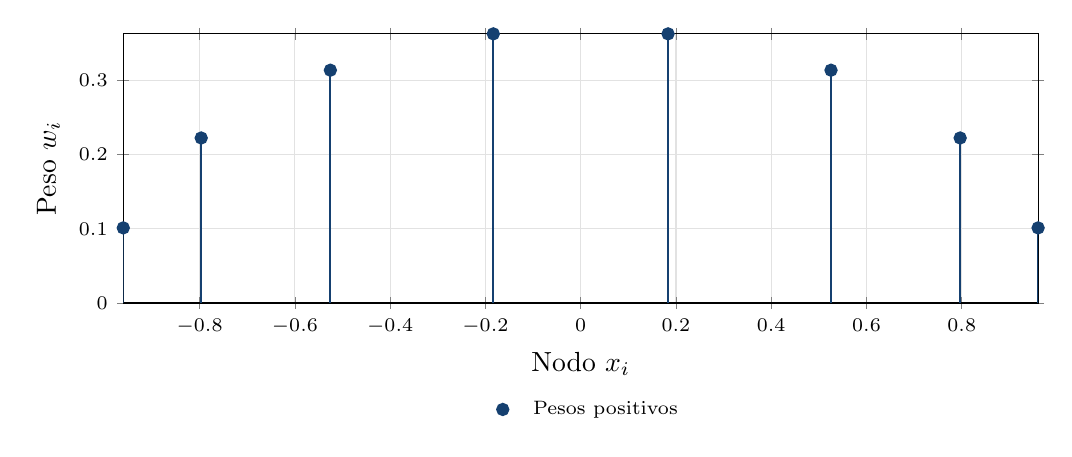
\begin{tikzpicture}\begin{axis}[base,axis lines=box,grid=major,minor tick num=0,width=13.2cm,height=5.0cm,xlabel={Nodo $x_i$},ylabel={Peso $w_i$},ymin=0,legend style={at={(0.5,-0.32)},anchor=north,legend columns=2,font=\scriptsize,draw=none,fill=white}]
\addplot[thick,azul,ycomb,mark=*] coordinates {(-0.9602898565,0.1012285363) (-0.7966664774,0.2223810345) (-0.5255324099,0.3137066459) (-0.1834346425,0.3626837834) (0.1834346425,0.3626837834) (0.5255324099,0.3137066459) (0.7966664774,0.2223810345) (0.9602898565,0.1012285363)};
\addlegendentry{Pesos positivos}
\end{axis}\end{tikzpicture}
\caption{Nodos y pesos de Gauss--Legendre con ocho puntos. La simetría de la medida se refleja en pares de nodos y pesos.}\label{fig:cdf-9}\end{figure}

\section{Newton para ceros: cuándo converge}
Para resolver $p(x)=0$,
\[
x_{k+1}=x_k-\frac{p(x_k)}{p'(x_k)}.
\]
Si $r$ es una raíz simple y $x_k$ suficientemente próximo, Taylor produce
\[
e_{k+1}=\frac{p''(r)}{2p'(r)}e_k^2+O(e_k^3),
\quad e_k=x_k-r.
\]
La convergencia cuadrática es local. Un punto inicial lejano puede converger a otra raíz, salir del intervalo o encontrar una derivada pequeña.

Para Legendre se pueden iniciar raíces mediante ángulos aproximados; después se verifica que cada una pertenezca a su intervalo aislado. Bisección o entrelazamiento mantienen una garantía global. Una tolerancia en $|p(x)|$ no equivale a tolerancia en $|x-r|$ sin conocer $|p'(r)|$.

Diferenciar la recurrencia permite obtener $p,p'$ juntos. Para grados altos se reescala para evitar valores enormes. El residuo, el intervalo de aislamiento y la simetría constituyen comprobaciones diferentes.






\begin{figure}[htbp]\centering
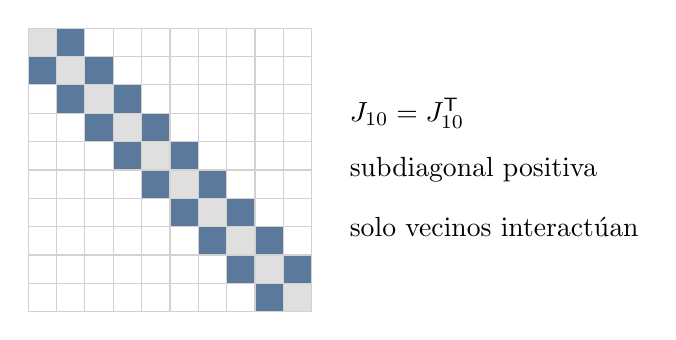
\begin{tikzpicture}[x=.36cm,y=.36cm]
\filldraw[fill=gray!25,draw=gray!35] (0,9) rectangle ++(1,1);
\filldraw[fill=azul!70,draw=gray!35] (1,9) rectangle ++(1,1);
\filldraw[fill=white,draw=gray!35] (2,9) rectangle ++(1,1);
\filldraw[fill=white,draw=gray!35] (3,9) rectangle ++(1,1);
\filldraw[fill=white,draw=gray!35] (4,9) rectangle ++(1,1);
\filldraw[fill=white,draw=gray!35] (5,9) rectangle ++(1,1);
\filldraw[fill=white,draw=gray!35] (6,9) rectangle ++(1,1);
\filldraw[fill=white,draw=gray!35] (7,9) rectangle ++(1,1);
\filldraw[fill=white,draw=gray!35] (8,9) rectangle ++(1,1);
\filldraw[fill=white,draw=gray!35] (9,9) rectangle ++(1,1);
\filldraw[fill=azul!70,draw=gray!35] (0,8) rectangle ++(1,1);
\filldraw[fill=gray!25,draw=gray!35] (1,8) rectangle ++(1,1);
\filldraw[fill=azul!70,draw=gray!35] (2,8) rectangle ++(1,1);
\filldraw[fill=white,draw=gray!35] (3,8) rectangle ++(1,1);
\filldraw[fill=white,draw=gray!35] (4,8) rectangle ++(1,1);
\filldraw[fill=white,draw=gray!35] (5,8) rectangle ++(1,1);
\filldraw[fill=white,draw=gray!35] (6,8) rectangle ++(1,1);
\filldraw[fill=white,draw=gray!35] (7,8) rectangle ++(1,1);
\filldraw[fill=white,draw=gray!35] (8,8) rectangle ++(1,1);
\filldraw[fill=white,draw=gray!35] (9,8) rectangle ++(1,1);
\filldraw[fill=white,draw=gray!35] (0,7) rectangle ++(1,1);
\filldraw[fill=azul!70,draw=gray!35] (1,7) rectangle ++(1,1);
\filldraw[fill=gray!25,draw=gray!35] (2,7) rectangle ++(1,1);
\filldraw[fill=azul!70,draw=gray!35] (3,7) rectangle ++(1,1);
\filldraw[fill=white,draw=gray!35] (4,7) rectangle ++(1,1);
\filldraw[fill=white,draw=gray!35] (5,7) rectangle ++(1,1);
\filldraw[fill=white,draw=gray!35] (6,7) rectangle ++(1,1);
\filldraw[fill=white,draw=gray!35] (7,7) rectangle ++(1,1);
\filldraw[fill=white,draw=gray!35] (8,7) rectangle ++(1,1);
\filldraw[fill=white,draw=gray!35] (9,7) rectangle ++(1,1);
\filldraw[fill=white,draw=gray!35] (0,6) rectangle ++(1,1);
\filldraw[fill=white,draw=gray!35] (1,6) rectangle ++(1,1);
\filldraw[fill=azul!70,draw=gray!35] (2,6) rectangle ++(1,1);
\filldraw[fill=gray!25,draw=gray!35] (3,6) rectangle ++(1,1);
\filldraw[fill=azul!70,draw=gray!35] (4,6) rectangle ++(1,1);
\filldraw[fill=white,draw=gray!35] (5,6) rectangle ++(1,1);
\filldraw[fill=white,draw=gray!35] (6,6) rectangle ++(1,1);
\filldraw[fill=white,draw=gray!35] (7,6) rectangle ++(1,1);
\filldraw[fill=white,draw=gray!35] (8,6) rectangle ++(1,1);
\filldraw[fill=white,draw=gray!35] (9,6) rectangle ++(1,1);
\filldraw[fill=white,draw=gray!35] (0,5) rectangle ++(1,1);
\filldraw[fill=white,draw=gray!35] (1,5) rectangle ++(1,1);
\filldraw[fill=white,draw=gray!35] (2,5) rectangle ++(1,1);
\filldraw[fill=azul!70,draw=gray!35] (3,5) rectangle ++(1,1);
\filldraw[fill=gray!25,draw=gray!35] (4,5) rectangle ++(1,1);
\filldraw[fill=azul!70,draw=gray!35] (5,5) rectangle ++(1,1);
\filldraw[fill=white,draw=gray!35] (6,5) rectangle ++(1,1);
\filldraw[fill=white,draw=gray!35] (7,5) rectangle ++(1,1);
\filldraw[fill=white,draw=gray!35] (8,5) rectangle ++(1,1);
\filldraw[fill=white,draw=gray!35] (9,5) rectangle ++(1,1);
\filldraw[fill=white,draw=gray!35] (0,4) rectangle ++(1,1);
\filldraw[fill=white,draw=gray!35] (1,4) rectangle ++(1,1);
\filldraw[fill=white,draw=gray!35] (2,4) rectangle ++(1,1);
\filldraw[fill=white,draw=gray!35] (3,4) rectangle ++(1,1);
\filldraw[fill=azul!70,draw=gray!35] (4,4) rectangle ++(1,1);
\filldraw[fill=gray!25,draw=gray!35] (5,4) rectangle ++(1,1);
\filldraw[fill=azul!70,draw=gray!35] (6,4) rectangle ++(1,1);
\filldraw[fill=white,draw=gray!35] (7,4) rectangle ++(1,1);
\filldraw[fill=white,draw=gray!35] (8,4) rectangle ++(1,1);
\filldraw[fill=white,draw=gray!35] (9,4) rectangle ++(1,1);
\filldraw[fill=white,draw=gray!35] (0,3) rectangle ++(1,1);
\filldraw[fill=white,draw=gray!35] (1,3) rectangle ++(1,1);
\filldraw[fill=white,draw=gray!35] (2,3) rectangle ++(1,1);
\filldraw[fill=white,draw=gray!35] (3,3) rectangle ++(1,1);
\filldraw[fill=white,draw=gray!35] (4,3) rectangle ++(1,1);
\filldraw[fill=azul!70,draw=gray!35] (5,3) rectangle ++(1,1);
\filldraw[fill=gray!25,draw=gray!35] (6,3) rectangle ++(1,1);
\filldraw[fill=azul!70,draw=gray!35] (7,3) rectangle ++(1,1);
\filldraw[fill=white,draw=gray!35] (8,3) rectangle ++(1,1);
\filldraw[fill=white,draw=gray!35] (9,3) rectangle ++(1,1);
\filldraw[fill=white,draw=gray!35] (0,2) rectangle ++(1,1);
\filldraw[fill=white,draw=gray!35] (1,2) rectangle ++(1,1);
\filldraw[fill=white,draw=gray!35] (2,2) rectangle ++(1,1);
\filldraw[fill=white,draw=gray!35] (3,2) rectangle ++(1,1);
\filldraw[fill=white,draw=gray!35] (4,2) rectangle ++(1,1);
\filldraw[fill=white,draw=gray!35] (5,2) rectangle ++(1,1);
\filldraw[fill=azul!70,draw=gray!35] (6,2) rectangle ++(1,1);
\filldraw[fill=gray!25,draw=gray!35] (7,2) rectangle ++(1,1);
\filldraw[fill=azul!70,draw=gray!35] (8,2) rectangle ++(1,1);
\filldraw[fill=white,draw=gray!35] (9,2) rectangle ++(1,1);
\filldraw[fill=white,draw=gray!35] (0,1) rectangle ++(1,1);
\filldraw[fill=white,draw=gray!35] (1,1) rectangle ++(1,1);
\filldraw[fill=white,draw=gray!35] (2,1) rectangle ++(1,1);
\filldraw[fill=white,draw=gray!35] (3,1) rectangle ++(1,1);
\filldraw[fill=white,draw=gray!35] (4,1) rectangle ++(1,1);
\filldraw[fill=white,draw=gray!35] (5,1) rectangle ++(1,1);
\filldraw[fill=white,draw=gray!35] (6,1) rectangle ++(1,1);
\filldraw[fill=azul!70,draw=gray!35] (7,1) rectangle ++(1,1);
\filldraw[fill=gray!25,draw=gray!35] (8,1) rectangle ++(1,1);
\filldraw[fill=azul!70,draw=gray!35] (9,1) rectangle ++(1,1);
\filldraw[fill=white,draw=gray!35] (0,0) rectangle ++(1,1);
\filldraw[fill=white,draw=gray!35] (1,0) rectangle ++(1,1);
\filldraw[fill=white,draw=gray!35] (2,0) rectangle ++(1,1);
\filldraw[fill=white,draw=gray!35] (3,0) rectangle ++(1,1);
\filldraw[fill=white,draw=gray!35] (4,0) rectangle ++(1,1);
\filldraw[fill=white,draw=gray!35] (5,0) rectangle ++(1,1);
\filldraw[fill=white,draw=gray!35] (6,0) rectangle ++(1,1);
\filldraw[fill=white,draw=gray!35] (7,0) rectangle ++(1,1);
\filldraw[fill=azul!70,draw=gray!35] (8,0) rectangle ++(1,1);
\filldraw[fill=gray!25,draw=gray!35] (9,0) rectangle ++(1,1);
\node[right] at (11,7) {$J_{10}=J_{10}^{\mathsf T}$};
\node[right] at (11,5) {subdiagonal positiva};
\node[right] at (11,3) {solo vecinos interactúan};
\end{tikzpicture}
\caption{Estructura de la matriz de Jacobi: diagonal gris, entradas vecinas azules y demás entradas nulas. La recurrencia de tres términos produce una matriz dispersa simétrica.}\label{fig:cdf-10}\end{figure}

\section{Estabilidad espectral y costo}
Para matrices simétricas, una perturbación $E$ desplaza autovalores a lo sumo $\norm E_2$ en sentido ordenado. La simetría evita autovalores complejos creados por una representación arbitraria. Los autovectores son más sensibles si hay autovalores cercanos; esto afecta pesos derivados de sus componentes.

Golub--Welsch con rutinas tridiagonales suele tener costo de orden $n^2$ para obtener todos los datos, dependiendo del algoritmo y de las salidas solicitadas. Usar un eigensolver denso desperdicia la estructura. Para reglas enormes existen métodos basados en ecuaciones diferenciales y expansiones asintóticas que reducen trabajo.

El artículo de Gil, Segura y Temme de 2019 desarrolla procesos iterativos especializados para Hermite y Laguerre. Su principio no es una sustitución de la teoría Gauss: conserva los mismos nodos exactos y modifica cómo se calculan.

\section{Gauss--Radau y Gauss--Lobatto}
Si se obliga a incluir un extremo, se obtiene una regla Radau: con $n$ nodos, la máxima exactitud genérica es $2n-2$. Si se incluyen ambos extremos, Lobatto alcanza $2n-3$. Las restricciones consumen grados de libertad.

Para Legendre Lobatto con tres nodos, los nodos son $-1,0,1$ y pesos $1/3,4/3,1/3$: es Simpson. Los nodos interiores generales son ceros de $P_{n-1}'$. Para Radau se modifica la familia mediante una condición en el extremo.

Estas reglas son útiles cuando ya se conocen evaluaciones de borde o cuando discretizamos ecuaciones con condiciones de frontera. Para una densidad singular en cero, forzar el extremo puede ser inconveniente. Una regla abierta o una transformación evita evaluar una infinidad integrable.

\section{Gauss--Hermite no integra automáticamente una CDF}
Es tentador escribir
$\Phi(z)=\E[\ind_{\{Z\le z\}}]$ y usar Gauss--Hermite. Sin embargo, el integrando es un escalón. Al mover $z$, la suma salta cada vez que cruza un nodo:
\[
\widehat\Phi_n(z)=\frac1{\sqrt\pi}\sum_iw_i
\ind_{\{\sqrt2x_i\le z\}}.
\]
No es una curva suave y puede aproximar mal una CDF puntual. La exactitud polinómica no se aplica a indicadores.

Una alternativa es transformar $\int_0^z\ph$ a $[-1,1]$ y aplicar Legendre a un integrando analítico. Otra es representar directamente la cola con un integrando positivo suave en $(0,\infty)$. El peso óptimo depende de la representación escogida.

La misma advertencia vale para gamma/Laguerre y beta/Jacobi: una expectativa suave suele beneficiarse enormemente de la cuadratura ponderada, pero una CDF requiere tratar su frontera de integración.

\section{De una regla unidimensional a una matriz tensorial}
En dimensión $d$, una regla producto tiene
\[
\int_{\R^d}f(x)\prod_{j=1}^dw_j(x_j)\dd x
\approx\sum_{i_1=1}^{n_1}\cdots\sum_{i_d=1}^{n_d}
\left(\prod_{j=1}^dw_{i_j}^{(j)}\right)
f(x_{i_1}^{(1)},\ldots,x_{i_d}^{(d)}).
\]
Si cada dimensión tiene $n$ nodos, necesita $n^d$ evaluaciones. Para $n=10,d=8$, son cien millones. La precisión unidimensional no elimina la maldición de dimensionalidad.

La distribución normal correlacionada no factoriza en las coordenadas originales. Cholesky puede transformar a normales independientes, pero la región de una CDF se convierte en desigualdades acopladas. Más adelante usaremos integración condicional, muestreo y cuasi Monte Carlo.

\section{Protocolo de verificación de una regla}
Una regla calculada debe comprobar:
\[
w_i>0,\quad x_i\in(a,b),\quad
\sum_iw_i=\mu_0,\quad
\sum_iw_ix_i^k\approx\mu_k,\quad k\le2n-1.
\]
Los momentos altos pueden estar mal escalados, por lo que es mejor comprobar una base ortogonal cuando sea posible. En Legendre, la simetría exige $x_i=-x_{n+1-i}$ y pesos iguales en parejas.

Probar solo $\int1$ no comprueba la exactitud completa. Probar polinomios no demuestra precisión para una función con singularidad fuera del dominio. Las verificaciones estructurales y las pruebas del integrando objetivo se complementan.

Si $w_i$ tienen una escala enorme, se normalizan por $\mu_0$ y se verifica una distribución de pesos que suma uno. Un sistema con salidas logarítmicas debe comprobar también el rango representable de las probabilidades.


\parte{VI. Aproximación espectral y cuadratura de Chebyshev}
\section{De Fourier a una serie de polinomios}
Si $f$ es continua en $[-1,1]$, definimos $g(\theta)=f(\cos\theta)$, que es par y periódica al extenderla. Una serie coseno
\[
g(\theta)=\frac{a_0}2+\sum_{k=1}^\infty a_k\cos(k\theta)
\]
se convierte en
\[
f(x)=\frac{a_0}2+\sum_{k=1}^\infty a_kT_k(x),\quad
a_k=\frac2\pi\int_0^\pi f(\cos\theta)\cos(k\theta)\dd\theta.
\]
Con regularidad adecuada, la serie converge a $f$; para funciones analíticas los coeficientes decaen geométricamente. La fórmula no afirma convergencia uniforme para cualquier función sin hipótesis.

El término constante tiene factor $1/2$ por la norma distinta de $T_0$. Si almacenamos directamente $c_0=a_0/2$, escribimos $f=\sum c_kT_k$ y desaparece ese factor. Cada algoritmo debe declarar su convención.

Para $f(x)=x^2$, $x^2=(T_2+T_0)/2$. Los coeficientes son $a_0=1,a_2=1/2$ y los demás cero. Integrar esta expansión dará $2/3$ sin muestrear.






\begin{figure}[htbp]\centering
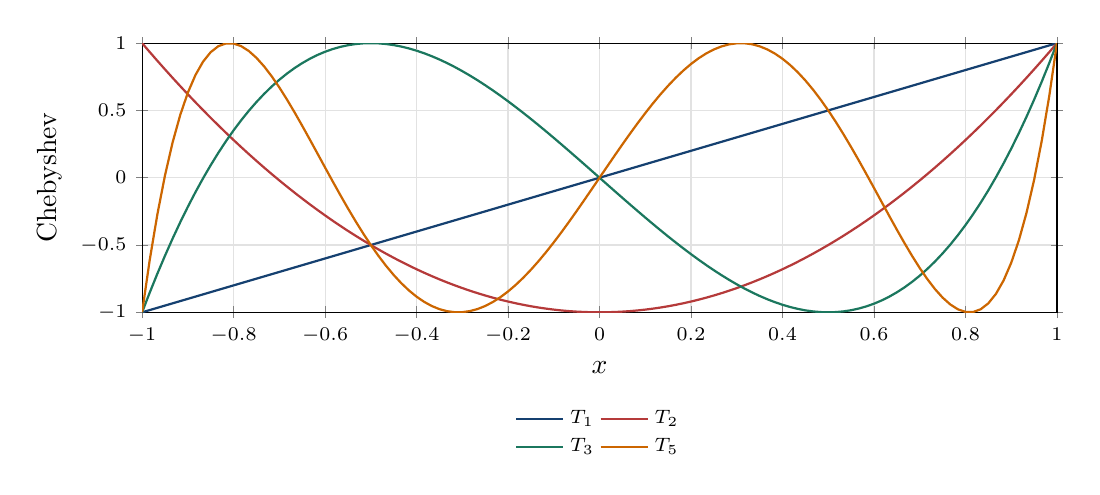
\begin{tikzpicture}\begin{axis}[base,axis lines=box,grid=major,minor tick num=0,width=13.2cm,height=5.0cm,xlabel={$x$},ylabel={Chebyshev},legend style={at={(0.5,-0.32)},anchor=north,legend columns=2,font=\scriptsize,draw=none,fill=white}]
\addplot[thick,azul,] coordinates {(-1,-1) (-0.9833333333,-0.9833333333) (-0.9666666667,-0.9666666667) (-0.95,-0.95) (-0.9333333333,-0.9333333333) (-0.9166666667,-0.9166666667) (-0.9,-0.9) (-0.8833333333,-0.8833333333) (-0.8666666667,-0.8666666667) (-0.85,-0.85) (-0.8333333333,-0.8333333333) (-0.8166666667,-0.8166666667) (-0.8,-0.8) (-0.7833333333,-0.7833333333) (-0.7666666667,-0.7666666667) (-0.75,-0.75) (-0.7333333333,-0.7333333333) (-0.7166666667,-0.7166666667) (-0.7,-0.7) (-0.6833333333,-0.6833333333) (-0.6666666667,-0.6666666667) (-0.65,-0.65) (-0.6333333333,-0.6333333333) (-0.6166666667,-0.6166666667) (-0.6,-0.6) (-0.5833333333,-0.5833333333) (-0.5666666667,-0.5666666667) (-0.55,-0.55) (-0.5333333333,-0.5333333333) (-0.5166666667,-0.5166666667) (-0.5,-0.5) (-0.4833333333,-0.4833333333) (-0.4666666667,-0.4666666667) (-0.45,-0.45) (-0.4333333333,-0.4333333333) (-0.4166666667,-0.4166666667) (-0.4,-0.4) (-0.3833333333,-0.3833333333) (-0.3666666667,-0.3666666667) (-0.35,-0.35) (-0.3333333333,-0.3333333333) (-0.3166666667,-0.3166666667) (-0.3,-0.3) (-0.2833333333,-0.2833333333) (-0.2666666667,-0.2666666667) (-0.25,-0.25) (-0.2333333333,-0.2333333333) (-0.2166666667,-0.2166666667) (-0.2,-0.2) (-0.1833333333,-0.1833333333) (-0.1666666667,-0.1666666667) (-0.15,-0.15) (-0.1333333333,-0.1333333333) (-0.1166666667,-0.1166666667) (-0.1,-0.1) (-0.08333333333,-0.08333333333) (-0.06666666667,-0.06666666667) (-0.05,-0.05) (-0.03333333333,-0.03333333333) (-0.01666666667,-0.01666666667) (0,6.123233996e-17) (0.01666666667,0.01666666667) (0.03333333333,0.03333333333) (0.05,0.05) (0.06666666667,0.06666666667) (0.08333333333,0.08333333333) (0.1,0.1) (0.1166666667,0.1166666667) (0.1333333333,0.1333333333) (0.15,0.15) (0.1666666667,0.1666666667) (0.1833333333,0.1833333333) (0.2,0.2) (0.2166666667,0.2166666667) (0.2333333333,0.2333333333) (0.25,0.25) (0.2666666667,0.2666666667) (0.2833333333,0.2833333333) (0.3,0.3) (0.3166666667,0.3166666667) (0.3333333333,0.3333333333) (0.35,0.35) (0.3666666667,0.3666666667) (0.3833333333,0.3833333333) (0.4,0.4) (0.4166666667,0.4166666667) (0.4333333333,0.4333333333) (0.45,0.45) (0.4666666667,0.4666666667) (0.4833333333,0.4833333333) (0.5,0.5) (0.5166666667,0.5166666667) (0.5333333333,0.5333333333) (0.55,0.55) (0.5666666667,0.5666666667) (0.5833333333,0.5833333333) (0.6,0.6) (0.6166666667,0.6166666667) (0.6333333333,0.6333333333) (0.65,0.65) (0.6666666667,0.6666666667) (0.6833333333,0.6833333333) (0.7,0.7) (0.7166666667,0.7166666667) (0.7333333333,0.7333333333) (0.75,0.75) (0.7666666667,0.7666666667) (0.7833333333,0.7833333333) (0.8,0.8) (0.8166666667,0.8166666667) (0.8333333333,0.8333333333) (0.85,0.85) (0.8666666667,0.8666666667) (0.8833333333,0.8833333333) (0.9,0.9) (0.9166666667,0.9166666667) (0.9333333333,0.9333333333) (0.95,0.95) (0.9666666667,0.9666666667) (0.9833333333,0.9833333333) (1,1)};
\addlegendentry{$T_1$}
\addplot[thick,rojo,] coordinates {(-1,1) (-0.9833333333,0.9338888889) (-0.9666666667,0.8688888889) (-0.95,0.805) (-0.9333333333,0.7422222222) (-0.9166666667,0.6805555556) (-0.9,0.62) (-0.8833333333,0.5605555556) (-0.8666666667,0.5022222222) (-0.85,0.445) (-0.8333333333,0.3888888889) (-0.8166666667,0.3338888889) (-0.8,0.28) (-0.7833333333,0.2272222222) (-0.7666666667,0.1755555556) (-0.75,0.125) (-0.7333333333,0.07555555556) (-0.7166666667,0.02722222222) (-0.7,-0.02) (-0.6833333333,-0.06611111111) (-0.6666666667,-0.1111111111) (-0.65,-0.155) (-0.6333333333,-0.1977777778) (-0.6166666667,-0.2394444444) (-0.6,-0.28) (-0.5833333333,-0.3194444444) (-0.5666666667,-0.3577777778) (-0.55,-0.395) (-0.5333333333,-0.4311111111) (-0.5166666667,-0.4661111111) (-0.5,-0.5) (-0.4833333333,-0.5327777778) (-0.4666666667,-0.5644444444) (-0.45,-0.595) (-0.4333333333,-0.6244444444) (-0.4166666667,-0.6527777778) (-0.4,-0.68) (-0.3833333333,-0.7061111111) (-0.3666666667,-0.7311111111) (-0.35,-0.755) (-0.3333333333,-0.7777777778) (-0.3166666667,-0.7994444444) (-0.3,-0.82) (-0.2833333333,-0.8394444444) (-0.2666666667,-0.8577777778) (-0.25,-0.875) (-0.2333333333,-0.8911111111) (-0.2166666667,-0.9061111111) (-0.2,-0.92) (-0.1833333333,-0.9327777778) (-0.1666666667,-0.9444444444) (-0.15,-0.955) (-0.1333333333,-0.9644444444) (-0.1166666667,-0.9727777778) (-0.1,-0.98) (-0.08333333333,-0.9861111111) (-0.06666666667,-0.9911111111) (-0.05,-0.995) (-0.03333333333,-0.9977777778) (-0.01666666667,-0.9994444444) (0,-1) (0.01666666667,-0.9994444444) (0.03333333333,-0.9977777778) (0.05,-0.995) (0.06666666667,-0.9911111111) (0.08333333333,-0.9861111111) (0.1,-0.98) (0.1166666667,-0.9727777778) (0.1333333333,-0.9644444444) (0.15,-0.955) (0.1666666667,-0.9444444444) (0.1833333333,-0.9327777778) (0.2,-0.92) (0.2166666667,-0.9061111111) (0.2333333333,-0.8911111111) (0.25,-0.875) (0.2666666667,-0.8577777778) (0.2833333333,-0.8394444444) (0.3,-0.82) (0.3166666667,-0.7994444444) (0.3333333333,-0.7777777778) (0.35,-0.755) (0.3666666667,-0.7311111111) (0.3833333333,-0.7061111111) (0.4,-0.68) (0.4166666667,-0.6527777778) (0.4333333333,-0.6244444444) (0.45,-0.595) (0.4666666667,-0.5644444444) (0.4833333333,-0.5327777778) (0.5,-0.5) (0.5166666667,-0.4661111111) (0.5333333333,-0.4311111111) (0.55,-0.395) (0.5666666667,-0.3577777778) (0.5833333333,-0.3194444444) (0.6,-0.28) (0.6166666667,-0.2394444444) (0.6333333333,-0.1977777778) (0.65,-0.155) (0.6666666667,-0.1111111111) (0.6833333333,-0.06611111111) (0.7,-0.02) (0.7166666667,0.02722222222) (0.7333333333,0.07555555556) (0.75,0.125) (0.7666666667,0.1755555556) (0.7833333333,0.2272222222) (0.8,0.28) (0.8166666667,0.3338888889) (0.8333333333,0.3888888889) (0.85,0.445) (0.8666666667,0.5022222222) (0.8833333333,0.5605555556) (0.9,0.62) (0.9166666667,0.6805555556) (0.9333333333,0.7422222222) (0.95,0.805) (0.9666666667,0.8688888889) (0.9833333333,0.9338888889) (1,1)};
\addlegendentry{$T_2$}
\addplot[thick,verde,] coordinates {(-1,-1) (-0.9833333333,-0.8533148148) (-0.9666666667,-0.7131851852) (-0.95,-0.5795) (-0.9333333333,-0.4521481481) (-0.9166666667,-0.3310185185) (-0.9,-0.216) (-0.8833333333,-0.1069814815) (-0.8666666667,-0.003851851852) (-0.85,0.0935) (-0.8333333333,0.1851851852) (-0.8166666667,0.2713148148) (-0.8,0.352) (-0.7833333333,0.4273518519) (-0.7666666667,0.4974814815) (-0.75,0.5625) (-0.7333333333,0.6225185185) (-0.7166666667,0.6776481481) (-0.7,0.728) (-0.6833333333,0.7736851852) (-0.6666666667,0.8148148148) (-0.65,0.8515) (-0.6333333333,0.8838518519) (-0.6166666667,0.9119814815) (-0.6,0.936) (-0.5833333333,0.9560185185) (-0.5666666667,0.9721481481) (-0.55,0.9845) (-0.5333333333,0.9931851852) (-0.5166666667,0.9983148148) (-0.5,1) (-0.4833333333,0.9983518519) (-0.4666666667,0.9934814815) (-0.45,0.9855) (-0.4333333333,0.9745185185) (-0.4166666667,0.9606481481) (-0.4,0.944) (-0.3833333333,0.9246851852) (-0.3666666667,0.9028148148) (-0.35,0.8785) (-0.3333333333,0.8518518519) (-0.3166666667,0.8229814815) (-0.3,0.792) (-0.2833333333,0.7590185185) (-0.2666666667,0.7241481481) (-0.25,0.6875) (-0.2333333333,0.6491851852) (-0.2166666667,0.6093148148) (-0.2,0.568) (-0.1833333333,0.5253518519) (-0.1666666667,0.4814814815) (-0.15,0.4365) (-0.1333333333,0.3905185185) (-0.1166666667,0.3436481481) (-0.1,0.296) (-0.08333333333,0.2476851852) (-0.06666666667,0.1988148148) (-0.05,0.1495) (-0.03333333333,0.09985185185) (-0.01666666667,0.04998148148) (0,-1.836970199e-16) (0.01666666667,-0.04998148148) (0.03333333333,-0.09985185185) (0.05,-0.1495) (0.06666666667,-0.1988148148) (0.08333333333,-0.2476851852) (0.1,-0.296) (0.1166666667,-0.3436481481) (0.1333333333,-0.3905185185) (0.15,-0.4365) (0.1666666667,-0.4814814815) (0.1833333333,-0.5253518519) (0.2,-0.568) (0.2166666667,-0.6093148148) (0.2333333333,-0.6491851852) (0.25,-0.6875) (0.2666666667,-0.7241481481) (0.2833333333,-0.7590185185) (0.3,-0.792) (0.3166666667,-0.8229814815) (0.3333333333,-0.8518518519) (0.35,-0.8785) (0.3666666667,-0.9028148148) (0.3833333333,-0.9246851852) (0.4,-0.944) (0.4166666667,-0.9606481481) (0.4333333333,-0.9745185185) (0.45,-0.9855) (0.4666666667,-0.9934814815) (0.4833333333,-0.9983518519) (0.5,-1) (0.5166666667,-0.9983148148) (0.5333333333,-0.9931851852) (0.55,-0.9845) (0.5666666667,-0.9721481481) (0.5833333333,-0.9560185185) (0.6,-0.936) (0.6166666667,-0.9119814815) (0.6333333333,-0.8838518519) (0.65,-0.8515) (0.6666666667,-0.8148148148) (0.6833333333,-0.7736851852) (0.7,-0.728) (0.7166666667,-0.6776481481) (0.7333333333,-0.6225185185) (0.75,-0.5625) (0.7666666667,-0.4974814815) (0.7833333333,-0.4273518519) (0.8,-0.352) (0.8166666667,-0.2713148148) (0.8333333333,-0.1851851852) (0.85,-0.0935) (0.8666666667,0.003851851852) (0.8833333333,0.1069814815) (0.9,0.216) (0.9166666667,0.3310185185) (0.9333333333,0.4521481481) (0.95,0.5795) (0.9666666667,0.7131851852) (0.9833333333,0.8533148148) (1,1)};
\addlegendentry{$T_3$}
\addplot[thick,orange!80!black,] coordinates {(-1,-1) (-0.9833333333,-0.6104691152) (-0.9666666667,-0.2726906996) (-0.95,0.017005) (-0.9333333333,0.2621445267) (-0.9166666667,0.4661136831) (-0.9,0.63216) (-0.8833333333,0.7633952058) (-0.8666666667,0.8627976955) (-0.85,0.933215) (-0.8333333333,0.9773662551) (-0.8166666667,0.9978446708) (-0.8,0.99712) (-0.7833333333,0.9775410082) (-0.7666666667,0.9413379424) (-0.75,0.890625) (-0.7333333333,0.8274027984) (-0.7166666667,0.7535608436) (-0.7,0.67088) (-0.6833333333,0.5810349588) (-0.6666666667,0.4855967078) (-0.65,0.386035) (-0.6333333333,0.283720823) (-0.6166666667,0.1799288683) (-0.6,0.07584) (-0.5833333333,-0.02745627572) (-0.5666666667,-0.1289593416) (-0.55,-0.227755) (-0.5333333333,-0.3230130041) (-0.5166666667,-0.4139845885) (-0.5,-0.5) (-0.4833333333,-0.5804660288) (-0.4666666667,-0.6548635391) (-0.45,-0.722745) (-0.4333333333,-0.7837320165) (-0.4166666667,-0.8375128601) (-0.4,-0.88384) (-0.3833333333,-0.9225276337) (-0.3666666667,-0.9534492181) (-0.35,-0.976535) (-0.3333333333,-0.9917695473) (-0.3166666667,-0.9991892798) (-0.3,-0.99888) (-0.2833333333,-0.9909744239) (-0.2666666667,-0.9756497119) (-0.25,-0.953125) (-0.2333333333,-0.92365893) (-0.2166666667,-0.8875471811) (-0.2,-0.84512) (-0.1833333333,-0.7967397325) (-0.1666666667,-0.7427983539) (-0.15,-0.683715) (-0.1333333333,-0.6199334979) (-0.1166666667,-0.5519198971) (-0.1,-0.48016) (-0.08333333333,-0.405156893) (-0.06666666667,-0.3274284774) (-0.05,-0.247505) (-0.03333333333,-0.1659265844) (-0.01666666667,-0.08324076132) (0,3.061616998e-16) (0.01666666667,0.08324076132) (0.03333333333,0.1659265844) (0.05,0.247505) (0.06666666667,0.3274284774) (0.08333333333,0.405156893) (0.1,0.48016) (0.1166666667,0.5519198971) (0.1333333333,0.6199334979) (0.15,0.683715) (0.1666666667,0.7427983539) (0.1833333333,0.7967397325) (0.2,0.84512) (0.2166666667,0.8875471811) (0.2333333333,0.92365893) (0.25,0.953125) (0.2666666667,0.9756497119) (0.2833333333,0.9909744239) (0.3,0.99888) (0.3166666667,0.9991892798) (0.3333333333,0.9917695473) (0.35,0.976535) (0.3666666667,0.9534492181) (0.3833333333,0.9225276337) (0.4,0.88384) (0.4166666667,0.8375128601) (0.4333333333,0.7837320165) (0.45,0.722745) (0.4666666667,0.6548635391) (0.4833333333,0.5804660288) (0.5,0.5) (0.5166666667,0.4139845885) (0.5333333333,0.3230130041) (0.55,0.227755) (0.5666666667,0.1289593416) (0.5833333333,0.02745627572) (0.6,-0.07584) (0.6166666667,-0.1799288683) (0.6333333333,-0.283720823) (0.65,-0.386035) (0.6666666667,-0.4855967078) (0.6833333333,-0.5810349588) (0.7,-0.67088) (0.7166666667,-0.7535608436) (0.7333333333,-0.8274027984) (0.75,-0.890625) (0.7666666667,-0.9413379424) (0.7833333333,-0.9775410082) (0.8,-0.99712) (0.8166666667,-0.9978446708) (0.8333333333,-0.9773662551) (0.85,-0.933215) (0.8666666667,-0.8627976955) (0.8833333333,-0.7633952058) (0.9,-0.63216) (0.9166666667,-0.4661136831) (0.9333333333,-0.2621445267) (0.95,-0.017005) (0.9666666667,0.2726906996) (0.9833333333,0.6104691152) (1,1)};
\addlegendentry{$T_5$}
\end{axis}\end{tikzpicture}
\caption{Los Chebyshev están acotados por uno y presentan extremos alternantes. Esta geometría relaciona interpolación, series y minimax.}\label{fig:cdf-8}\end{figure}

\section{Coeficientes discretos y aliasing}
Tomemos $\theta_j=j\pi/N$ y valores $f_j=f(\cos\theta_j)$. Una transformación coseno discreta permite calcular coeficientes del interpolante de grado $N$ en esos nodos. Con pesos mitad en extremos,
\[
\widetilde a_k=\frac2N\sum_{j=0}^N{}''
f_j\cos(kj\pi/N).
\]
Los coeficientes extremos $k=0,N$ se usan con media ponderación al reconstruir. Los símbolos dobles indican que las contribuciones de $j=0,N$ valen la mitad.

La identidad $\cos((2N-k)\theta_j)=\cos(k\theta_j)$ explica aliasing: una frecuencia alta coincide con otra baja en la malla. Coeficientes discretos pequeños sugieren resolución, pero no prueban que no exista una oscilación escondida entre nodos.

Duplicar $N$ reutiliza valores de los nodos antiguos. Una FFT permite calcular la transformada rápidamente. El costo de construir la representación se amortiza si evaluamos una CDF para muchos valores del argumento.

\section{Clenshaw: Horner para una base ortogonal}
Para $p(x)=\sum_{k=0}^N c_kT_k(x)$, definimos $b_{N+1}=b_{N+2}=0$ y
\[
b_k=c_k+2xb_{k+1}-b_{k+2},\qquad k=N,\ldots,1.
\]
La salida es
\[
p(x)=c_0+xb_1-b_2.
\]
La prueba sustituye la recurrencia y usa $T_{k+1}=2xT_k-T_{k-1}$; todos los términos intermedios se cancelan. Para $N=2$, $b_2=c_2$, $b_1=c_1+2xc_2$, y la salida es
$c_0+c_1x+c_2(2x^2-1)$.

La complejidad es lineal y no construye cada $T_k$ por separado. Fuera de $[-1,1]$, los $T_k$ crecen y una representación buena en el intervalo puede extrapolar mal. No se deben aplicar coeficientes de un dominio a otro sin transformar $x$.

\section{Integrar una serie Chebyshev}
Con $x=\cos\theta$,
\[
\int_{-1}^1T_k(x)\dd x
=\int_0^\pi\cos(k\theta)\sin\theta\dd\theta.
\]
Para $k$ impar es cero por simetría. Para $k$ par,
\[
\int_{-1}^1T_k(x)\dd x=\frac2{1-k^2},
\]
incluyendo $k=0$. Por tanto, para $p=\sum c_kT_k$,
\[
\int_{-1}^1p(x)\dd x
=2c_0+\sum_{\substack{2\le k\le N\\k\ {\rm par}}}\frac{2c_k}{1-k^2}.
\]
Integrar el interpolante en nodos de extremos Chebyshev es Clenshaw--Curtis. Sus pesos para peso uno no son los de Gauss--Chebyshev.

El error puede analizarse por coeficientes y aliasing. Si $|c_k|\le C\rho^{-k}$ con $\rho>1$, el resto uniforme satisface
$\sum_{k>N}|c_k|\le C\rho^{-(N+1)}/(1-\rho^{-1})$. La integral del resto es a lo sumo dos veces esa cantidad. La cota vale para truncación exacta; el interpolante agrega aliasing y redondeo.

\section{Construir una primitiva espectral}
Para $k\ge2$,
\[
\int T_k(x)\dd x=
\frac{T_{k+1}(x)}{2(k+1)}-\frac{T_{k-1}(x)}{2(k-1)}+C.
\]
Se comprueba diferenciando o con $x=\cos\theta$. Los casos especiales son
$\int T_0=x$ y $\int T_1=x^2/2=(T_2+T_0)/4$.

Podemos transformar los coeficientes de una densidad en coeficientes de su integral. Después elegimos la constante para que la primitiva sea cero en el extremo izquierdo. Si la densidad se aproxima con error uniforme $\eta$ en $[a,b]$,
\[
|F(x)-\widehat F(x)|\le(x-a)\eta
\]
más el error de masa fuera del intervalo.

La CDF aproximada no es automáticamente creciente: un polinomio de densidad puede tener pequeñas partes negativas. Verificar no negatividad o usar una parametrización positiva puede ser necesario en aplicaciones que requieran una función de distribución válida y no solo una aproximación puntual.

\section{Elipse de Bernstein y convergencia geométrica}

Para comprender la analiticidad introducimos números complejos $z=x+iy$, con $i^2=-1$. La conjugada es $\overline z=x-iy$ y el módulo $|z|=\sqrt{x^2+y^2}$. Multiplicar y sumar se hace con esas reglas. La serie exponencial da
$e^{i\theta}=\cos\theta+i\sin\theta$, agrupando términos pares e impares; por tanto tiene módulo uno.

Una función es analítica en una región si admite una serie de potencias convergente alrededor de cada punto de ella. Una singularidad es un punto donde esa representación deja de ser válida. El teorema integral de Cauchy, resultado central del análisis complejo que aquí se declara, permite representar coeficientes mediante integrales sobre curvas cerradas. En un círculo de radio $\rho$, si $|g|\le M$, los coeficientes de Taylor satisfacen $|c_k|\le M/\rho^k$. La cota se deduce de la longitud $2\pi\rho$ de la curva y del denominador $\rho^{k+1}$ de la fórmula de Cauchy. Ese es el principio que trasladaremos de un círculo a una elipse.

Escribamos $z=(w+w^{-1})/2$ para $|w|=\rho>1$. La imagen es una elipse con focos $\pm1$, semiejes $(\rho+\rho^{-1})/2$ y $(\rho-\rho^{-1})/2$. Si $f$ es analítica dentro y sobre ella, con $|f|\le M$, una estimación mediante series de Laurent da
\[
|a_k|\le2M\rho^{-k}.
\]
La deducción usa $T_k(z)=(w^k+w^{-k})/2$ y la fórmula integral de Cauchy para los coeficientes. El teorema de Cauchy pertenece al análisis complejo; aquí se declara su uso y se deriva la consecuencia geométrica.

Una singularidad cercana limita $\rho$, lo que enlentece el decaimiento. Para $1/(1+25x^2)$, los polos en $\pm i/5$ fijan una elipse pequeña. Para una función entera, $\rho$ puede crecer, pero $M$ también: optimizar la cota exige equilibrarlos.

\section{Expansión uniforme no significa minimax}
La proyección $L^2$ minimiza error cuadrático ponderado. Un interpolante coincide en nodos. Una expansión truncada conserva coeficientes bajos. Un minimax minimiza el mayor error absoluto. Son cuatro objetivos distintos.

Si $p_N$ es una truncación Chebyshev, la cota de cola puede ser excelente y su error puede acercarse al óptimo uniforme. Pero no se debe afirmar que toda truncación sea el minimax exacto. La alternancia de extremos determinará cuándo lo es.

Para una densidad o una cola pequeña, un objetivo relativo puede ser más relevante:
\[
\min_p\max_{x\in[a,b]}\left|\frac{f(x)-p(x)}{f(x)}\right|.
\]
Esto equivale a un minimax ponderado con peso $1/f$ si $f$ no se anula. Cerca de ceros el problema necesita reformulación.

\section{Una transformación de cola a intervalo compacto}
El cociente de Mills $R(x)=\Q(x)/\ph(x)$ tiene $R(x)\sim1/x$. Para $x\ge A>0$, usemos $s=1/x$ o
$t=(x-A)/(x+A)\in[0,1)$. En vez de aproximar $\Q(x)$, que varía por cientos de órdenes de magnitud, aproximamos una cantidad de tamaño moderado:
\[
xR(x)\to1.
\]
Una aproximación racional o Chebyshev de $xR(x)$ puede evaluarse y luego combinarse con
$\log\ph(x)=-x^2/2-\log(2\pi)/2$.

La transformación crea un extremo correspondiente a infinito. La expansión asintótica no garantiza analiticidad en ese extremo; puede ser divergente. Aun así, dividir la cola en regiones finitas y una región asintótica ofrece un diseño eficaz.

\section{Métodos Sinc y trapecio en una recta transformada}
La función $\operatorname{sinc}(t)=\sin(\pi t)/(\pi t)$, con valor uno en cero, interpola una malla uniforme. Bajo hipótesis de analiticidad en una franja, las aproximaciones Sinc y el trapecio infinito tienen errores que decrecen rápidamente al reducir el paso.

En una recta transformada,
\[
I=\int_\R g(t)\dd t\approx h\sum_{k=-N}^Ng(kh).
\]
Hay dos escalas: ancho de franja analítica, que controla discretización, y velocidad de decaimiento, que controla truncamiento. Para una transformación doble exponencial, el segundo puede decrecer especialmente rápido.

Una reducción de error observada al pasar de $h$ a $h/2$ es útil pero no sustituye la hipótesis analítica. Una singularidad compleja cercana a la recta puede limitar la convergencia aunque el gráfico real parezca suave.

\section{Selección de métodos en un intervalo}
Para una integral suave y una sola evaluación, Gauss de orden moderado evita construir una representación global. Para muchas evaluaciones de una primitiva, representar la densidad o la CDF con Chebyshev puede amortizar el costo. Para singularidades de extremo, Jacobi o tanh--sinh pueden ser más apropiados.

La comparación requiere el mismo criterio de error y contabilizar evaluaciones, preparación de coeficientes y reutilización. Un método que es rápido después de precalcular mil coeficientes no tiene el mismo costo inicial que una llamada de serie de diez términos.

Un evaluador híbrido combina herramientas: serie en el origen, racional en un intervalo central, fracción continua en cola y forma logarítmica donde la probabilidad subdesborda. La arquitectura será deducida para cada función especial.


\parte{VII. Padé, minimax y fracciones continuas}
\section{Aproximación racional y normalización}
Una función racional es $r(x)=p_m(x)/q_n(x)$ con grados a lo sumo $m,n$. Multiplicar ambos por la misma constante no cambia la función. Usualmente fijamos $q_n(0)=1$ cuando sea posible, de modo que hay $m+n+1$ parámetros efectivos.

Un denominador nulo en el dominio crea un polo, salvo cancelación común exacta. Una cancelación aproximada no elimina necesariamente la sensibilidad. Antes de entregar una aproximación racional se debe comprobar que el denominador esté separado de cero en la región de uso.

Un racional puede representar un polo con pocos coeficientes, mientras un polinomio necesitaría muchos. Pero para una función sin polos reales, introducir polos cerca del intervalo es peligroso. Más flexibilidad no garantiza más estabilidad.

\section{Padé como un sistema de coeficientes}
Sea $f(x)=\sum_{k=0}^\infty c_kx^k$ cerca de cero. Un Padé $[m/n]$ satisface
\[
q_n(x)f(x)-p_m(x)=O(x^{m+n+1}),\qquad q_n(0)=1.
\]
Escribiendo $q_n=1+b_1x+\cdots+b_nx^n$, las ecuaciones para grados $k=m+1,\ldots,m+n$ son
\[
c_k+b_1c_{k-1}+\cdots+b_nc_{k-n}=0,
\]
con $c_j=0$ para $j<0$. Después,
\[
a_k=\sum_{j=0}^{\min(k,n)}b_jc_{k-j},\qquad b_0=1,\quad k=0,\ldots,m.
\]
La construcción es lineal en $b_j$ y luego en $a_k$. El sistema puede ser singular o dar grados efectivos menores. La existencia y unicidad requieren analizar el caso, no se deducen de contar ecuaciones.

Padé ajusta una serie local. No minimiza automáticamente el máximo error en un intervalo y no garantiza ausencia de polos. Debe validarse en el dominio donde se utilizará.

\section{Deducir dos Padé elementales}
Para $e^x$, $c_k=1/k!$. El Padé $[1/1]$ exige $1/2+b_1=0$, de modo que
\[
e^x\approx\frac{1+x/2}{1-x/2}.
\]
Tiene un polo en $x=2$, aunque $e^x$ no lo tiene. Sirve como aproximación local, no como fórmula global. Para $[2/2]$, las ecuaciones de grados tres y cuatro dan $b_1=-1/2,b_2=1/12$, y
\[
e^x\approx\frac{1+x/2+x^2/12}{1-x/2+x^2/12}.
\]
El error local comienza en grado cinco.

Para $\log(1+x)=x-x^2/2+x^3/3-\cdots$, el $[1/1]$ con numerador sin constante es
\[
\log(1+x)\approx\frac{x}{1+x/2}.
\]
Su coincidencia local es de orden tres. En $x$ cercano a $-1$, un polinomio o racional pequeño construido en cero no resuelve la singularidad logarítmica: transformar o dividir dominio sigue siendo necesario.

\section{Padé de la función error normalizada}
La simetría sugiere escribir
\[
\erf(x)=\frac{2x}{\sqrt\pi}\,G(x^2),\qquad
G(y)=\int_0^1e^{-yt^2}\dd t
=\sum_{k=0}^\infty\frac{(-y)^k}{k!(2k+1)}.
\]
Así $G(y)=1-y/3+y^2/10-y^3/42+\cdots$. Para $[1/1]$, $1/10-b_1/3=0$, por lo que $b_1=3/10$ y $a_1=-1/30$:
\[
G(y)\approx\frac{1-y/30}{1+3y/10}.
\]
En consecuencia,
\[
\erf(x)\approx\frac{2x}{\sqrt\pi}
\frac{1-x^2/30}{1+3x^2/10}.
\]
Respeta imparidad, pero para $x$ grande crece con signo negativo y no se acerca a uno. La construcción local no ha impuesto el comportamiento en infinito.

Para una cola, una alternativa es aproximar $\erfcx(x)=e^{x^2}\erfc(x)$, cuya magnitud es de orden $1/x$. Ajustar una función escalada evita obligar al racional a reproducir un exponencial extremadamente pequeño.






\begin{figure}[htbp]\centering
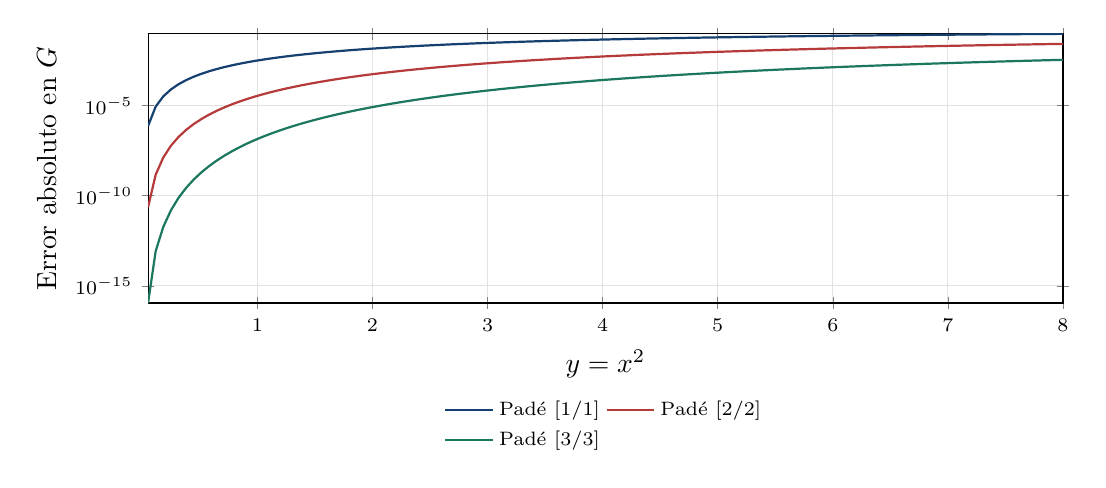
\begin{tikzpicture}\begin{axis}[base,axis lines=box,grid=major,minor tick num=0,width=13.2cm,height=5.0cm,ymode=log,xlabel={$y=x^2$},ylabel={Error absoluto en $G$},legend style={at={(0.5,-0.32)},anchor=north,legend columns=2,font=\scriptsize,draw=none,fill=white}]
\addplot[thick,azul,] coordinates {(0.05,7.470909063e-07) (0.11625,8.966705551e-06) (0.1825,3.314878018e-05) (0.24875,8.02455945e-05) (0.315,0.0001558614427) (0.38125,0.00026444061) (0.4475,0.0004094306611) (0.51375,0.0005934243571) (0.58,0.0008182830464) (0.64625,0.001085243975) (0.7125,0.001395013619) (0.77875,0.00174784886) (0.845,0.002143627569) (0.91125,0.002581909959) (0.9775,0.003061991884) (1.04375,0.003582951106) (1.11,0.004143687424) (1.17625,0.004742957431) (1.2425,0.005379404577) (1.30875,0.006051585134) (1.375,0.006757990565) (1.44125,0.007497066749) (1.5075,0.008267230468) (1.57375,0.00906688348) (1.64,0.009894424498) (1.70625,0.01074825933) (1.7725,0.01162680941) (1.83875,0.01252851894) (1.905,0.01345186078) (1.97125,0.01439534135) (2.0375,0.01535750449) (2.10375,0.01633693459) (2.17,0.01733225907) (2.23625,0.0183421501) (2.3025,0.01936532599) (2.36875,0.02040055196) (2.435,0.02144664063) (2.50125,0.02250245219) (2.5675,0.02356689418) (2.63375,0.02463892114) (2.7,0.02571753405) (2.76625,0.02680177952) (2.8325,0.02789074895) (2.89875,0.02898357751) (2.965,0.03007944306) (3.03125,0.03117756495) (3.0975,0.03227720286) (3.16375,0.0333776555) (3.23,0.03447825934) (3.29625,0.03557838732) (3.3625,0.03667744751) (3.42875,0.03777488184) (3.495,0.03887016478) (3.56125,0.03996280206) (3.6275,0.04105232939) (3.69375,0.04213831121) (3.76,0.04322033948) (3.82625,0.0442980325) (3.8925,0.04537103369) (3.95875,0.04643901052) (4.025,0.04750165335) (4.09125,0.04855867442) (4.1575,0.04960980678) (4.22375,0.05065480329) (4.29,0.05169343568) (4.35625,0.0527254936) (4.4225,0.05375078376) (4.48875,0.05476912901) (4.555,0.05578036756) (4.62125,0.05678435221) (4.6875,0.05778094949) (4.75375,0.05877003907) (4.82,0.05975151292) (4.88625,0.06072527477) (4.9525,0.06169123935) (5.01875,0.0626493319) (5.085,0.06359948749) (5.15125,0.06454165051) (5.2175,0.06547577413) (5.28375,0.06640181978) (5.35,0.0673197567) (5.41625,0.06822956145) (5.4825,0.06913121747) (5.54875,0.0700247147) (5.615,0.07091004913) (5.68125,0.07178722246) (5.7475,0.07265624175) (5.81375,0.07351711905) (5.88,0.07436987106) (5.94625,0.0752145189) (6.0125,0.07605108774) (6.07875,0.07687960655) (6.145,0.07770010786) (6.21125,0.07851262748) (6.2775,0.07931720427) (6.34375,0.08011387993) (6.41,0.08090269878) (6.47625,0.08168370758) (6.5425,0.0824569553) (6.60875,0.08322249295) (6.675,0.08398037347) (6.74125,0.08473065149) (6.8075,0.08547338322) (6.87375,0.0862086263) (6.94,0.08693643967) (7.00625,0.08765688344) (7.0725,0.08837001875) (7.13875,0.08907590772) (7.205,0.08977461324) (7.27125,0.09046619898) (7.3375,0.09115072921) (7.40375,0.09182826878) (7.47,0.09249888296) (7.53625,0.09316263745) (7.6025,0.09381959822) (7.66875,0.09446983151) (7.735,0.09511340372) (7.80125,0.09575038138) (7.8675,0.09638083106) (7.93375,0.09700481936) (8,0.09762241281)};
\addlegendentry{Padé $[1/1]$}
\addplot[thick,rojo,] coordinates {(0.05,2.315858616e-11) (0.11625,1.490303658e-09) (0.1825,1.346654299e-08) (0.24875,6.005726461e-08) (0.315,1.854752772e-07) (0.38125,4.570238026e-07) (0.4475,9.664568528e-07) (0.51375,1.830095868e-06) (0.58,3.188012119e-06) (0.64625,5.202526366e-06) (0.7125,8.056228872e-06) (0.77875,1.194968257e-05) (0.845,1.70989388e-05) (0.91125,2.373296734e-05) (0.9775,3.209107966e-05) (1.04375,4.242040564e-05) (1.11,5.497346878e-05) (1.17625,7.000589217e-05) (1.2425,8.777425788e-05) (1.30875,0.0001085341341) (1.375,0.0001325382777) (1.44125,0.0001600350156) (1.5075,0.0001912668036) (1.57375,0.0002264689585) (1.64,0.0002658685572) (1.70625,0.000309683496) (1.7725,0.0003581216989) (1.83875,0.0004113804672) (1.905,0.0004696459594) (1.97125,0.0005330927905) (2.0375,0.0006018837421) (2.10375,0.0006761695712) (2.17,0.0007560889101) (2.23625,0.0008417682459) (2.3025,0.0009333219729) (2.36875,0.001030852508) (2.435,0.001134450462) (2.50125,0.00124419486) (2.5675,0.001360153401) (2.63375,0.001482382756) (2.7,0.001610928896) (2.76625,0.001745827442) (2.8325,0.001887104035) (2.89875,0.002034774724) (2.965,0.002188846365) (3.03125,0.002349317027) (3.0975,0.002516176402) (3.16375,0.002689406223) (3.23,0.002868980672) (3.29625,0.0030548668) (3.3625,0.003247024926) (3.42875,0.003445409044) (3.495,0.003649967218) (3.56125,0.003860641967) (3.6275,0.00407737064) (3.69375,0.004300085789) (3.76,0.00452871552) (3.82625,0.004763183843) (3.8925,0.005003410997) (3.95875,0.005249313782) (4.025,0.005500805858) (4.09125,0.005757798049) (4.1575,0.006020198622) (4.22375,0.006287913561) (4.29,0.006560846825) (4.35625,0.006838900596) (4.4225,0.007121975514) (4.48875,0.0074099709) (4.555,0.007702784968) (4.62125,0.008000315023) (4.6875,0.008302457653) (4.75375,0.008609108908) (4.82,0.008920164464) (4.88625,0.009235519786) (4.9525,0.009555070272) (5.01875,0.009878711397) (5.085,0.01020633884) (5.15125,0.0105378486) (5.2175,0.01087313713) (5.28375,0.0112121014) (5.35,0.01155463905) (5.41625,0.01190064843) (5.4825,0.01225002872) (5.54875,0.01260267998) (5.615,0.01295850324) (5.68125,0.01331740055) (5.7475,0.01367927504) (5.81375,0.01404403099) (5.88,0.01441157386) (5.94625,0.01478181033) (6.0125,0.01515464837) (6.07875,0.01552999722) (6.145,0.01590776748) (6.21125,0.0162878711) (6.2775,0.0166702214) (6.34375,0.01705473311) (6.41,0.01744132237) (6.47625,0.01782990677) (6.5425,0.01822040531) (6.60875,0.01861273847) (6.675,0.01900682815) (6.74125,0.01940259772) (6.8075,0.01979997202) (6.87375,0.02019887733) (6.94,0.02059924138) (7.00625,0.02100099337) (7.0725,0.0214040639) (7.13875,0.02180838506) (7.205,0.02221389031) (7.27125,0.02262051456) (7.3375,0.02302819411) (7.40375,0.02343686665) (7.47,0.02384647126) (7.53625,0.02425694836) (7.6025,0.02466823974) (7.66875,0.02508028851) (7.735,0.0254930391) (7.80125,0.02590643723) (7.8675,0.02632042992) (7.93375,0.02673496543) (8,0.02714999329)};
\addlegendentry{Padé $[2/2]$}
\addplot[thick,verde,] coordinates {(0.05,1.110223025e-16) (0.11625,8.515410599e-14) (0.1825,1.89259719e-12) (0.24875,1.562783236e-11) (0.315,7.714473504e-11) (0.38125,2.77515233e-10) (0.4475,8.056971756e-10) (0.51375,2.003574084e-09) (0.58,4.431786604e-09) (0.64625,8.944271324e-09) (0.7125,1.676913952e-08) (0.77875,2.959345324e-08) (0.845,4.964952594e-08) (0.91125,7.980051908e-08) (0.9775,1.236233165e-07) (1.04375,1.854869307e-07) (1.11,2.70624941e-07) (1.17625,3.852007524e-07) (1.2425,5.36364728e-07) (1.30875,7.323024943e-07) (1.375,9.822739594e-07) (1.44125,1.296642787e-06) (1.5075,1.686896271e-06) (1.57375,2.165655691e-06) (1.64,2.746677411e-06) (1.70625,3.444845057e-06) (1.7725,4.276153223e-06) (1.83875,5.257683256e-06) (1.905,6.407571664e-06) (1.97125,7.744971808e-06) (2.0375,9.290009506e-06) (2.10375,1.106373322e-05) (2.17,1.308805951e-05) (2.23625,1.538571437e-05) (2.3025,1.798017117e-05) (2.36875,2.089558576e-05) (2.435,2.415672936e-05) (2.50125,2.778891986e-05) (2.5675,3.181795196e-05) (2.63375,3.627002679e-05) (2.7,4.117168135e-05) (2.76625,4.654971827e-05) (2.8325,5.243113632e-05) (2.89875,5.884306193e-05) (2.965,6.58126821e-05) (3.03125,7.336717895e-05) (3.0975,8.153366626e-05) (3.16375,9.033912804e-05) (3.23,9.981035949e-05) (3.29625,0.0001099739104) (3.3625,0.0001208560311) (3.42875,0.0001324826212) (3.495,0.0001448791812) (3.56125,0.0001580707665) (3.6275,0.0001720819448) (3.69375,0.0001869367562) (3.76,0.000202658676) (3.82625,0.0002192705805) (3.8925,0.000236794716) (3.95875,0.0002552526698) (4.025,0.0002746653448) (4.09125,0.000295052936) (4.1575,0.0003164349103) (4.22375,0.0003388299885) (4.29,0.0003622561298) (4.35625,0.0003867305185) (4.4225,0.0004122695535) (4.48875,0.000438888839) (4.555,0.0004666031788) (4.62125,0.0004954265708) (4.6875,0.0005253722052) (4.75375,0.0005564524626) (4.82,0.0005886789156) (4.88625,0.0006220623309) (4.9525,0.000656612673) (5.01875,0.0006923391098) (5.085,0.0007292500188) (5.15125,0.0007673529955) (5.2175,0.0008066548617) (5.28375,0.0008471616757) (5.35,0.0008888787436) (5.41625,0.0009318106306) (5.4825,0.000975961174) (5.54875,0.001021333496) (5.615,0.001067930019) (5.68125,0.001115752478) (5.7475,0.001164801938) (5.81375,0.001215078809) (5.88,0.001266582859) (5.94625,0.001319313235) (6.0125,0.001373268477) (6.07875,0.001428446534) (6.145,0.001484844784) (6.21125,0.001542460048) (6.2775,0.001601288608) (6.34375,0.001661326225) (6.41,0.001722568156) (6.47625,0.001785009173) (6.5425,0.001848643575) (6.60875,0.001913465211) (6.675,0.001979467495) (6.74125,0.002046643422) (6.8075,0.002114985584) (6.87375,0.002184486189) (6.94,0.002255137077) (7.00625,0.002326929733) (7.0725,0.002399855309) (7.13875,0.002473904633) (7.205,0.002549068228) (7.27125,0.002625336327) (7.3375,0.002702698888) (7.40375,0.002781145606) (7.47,0.002860665931) (7.53625,0.00294124908) (7.6025,0.003022884051) (7.66875,0.003105559635) (7.735,0.003189264431) (7.80125,0.003273986859) (7.8675,0.003359715169) (7.93375,0.003446437456) (8,0.003534141672)};
\addlegendentry{Padé $[3/3]$}
\end{axis}\end{tikzpicture}
\caption{Padé de la función error normalizada. Aumentar grados mejora este rango, pero la construcción sigue siendo local y requiere comprobar polos y error global.}\label{fig:cdf-12}\end{figure}

\section{Minimax uniforme y existencia}
En un intervalo compacto buscamos
\[
E_m=\min_{p\in\mathcal P_m}\norm{f-p}_\infty.
\]
Para $f$ continua, el mínimo existe. Una demostración toma una sucesión de polinomios con errores acotados y evalúa en $m+1$ nodos distintos. Esos valores están acotados; el sistema Vandermonde invertible implica coeficientes acotados. Extraemos una subsecuencia convergente en el espacio finito de coeficientes y pasamos al límite uniforme.

La norma uniforme mide el peor error, mientras la norma $L^2$ promedia su cuadrado. Un pico estrecho puede ser casi invisible en $L^2$ y dominar el error uniforme.

Para $f(x)=x^2$ en $[-1,1]$, una constante $c$ tiene error máximo $\max(|c|,|1-c|)$, mínimo en $c=1/2$ con $E=1/2$. La simetrización de cualquier recta $ax+b$ elimina $ax$ sin aumentar el error, por lo que la mejor recta también es $1/2$.

\section{Alternancia: suficiencia y necesidad}
El teorema de alternancia afirma que $p_m$ es el único mejor polinomio si y solo si existen $m+2$ puntos ordenados
$x_0<\cdots<x_{m+1}$ con
\[
f(x_i)-p_m(x_i)=(-1)^i\sigma E_m,\qquad \sigma\in\{-1,1\}.
\]
La suficiencia se prueba por raíces: si otro $q$ tuviera error estrictamente menor, $q-p$ tendría signos alternos en esos puntos. Por el teorema intermedio tendría al menos $m+1$ raíces, imposible para grado $\le m$.

La necesidad requiere mostrar que si los extremos máximos no forman suficiente alternancia, existe un polinomio de grado $\le m$ cuyo signo coincide con el error en los conjuntos de extremos. Una perturbación pequeña reduce el máximo sin crear otro mayor fuera de ellos, contradiciendo optimalidad. El argumento usa continuidad y compacidad para separar extremos y controlar el resto del intervalo.

El error puede tener más de $m+2$ extremos máximos; basta una subsecuencia alternante. No basta que oscile en varios puntos con amplitudes diferentes.

\section{Un minimax lineal de la exponencial, calculado}
En $[-1,1]$, buscamos $p(x)=ax+b$. El error $e^x-ax-b$ es convexo, así que el máximo se da en extremos y el mínimo interior cuando $e^\xi=a$. Igualar los dos errores externos exige
\[
e-a-b=e^{-1}+a-b,\qquad a=\sinh1.
\]
Entonces $\xi=\log a$ está dentro del intervalo. Igualando magnitudes,
\[
\cosh1-b=E,\qquad a-a\log a-b=-E.
\]
Por tanto
\[
b=\frac{\cosh1+a-a\log a}{2},\qquad
E=\frac{\cosh1-a+a\log a}{2}.
\]
Tenemos alternancia $+E,-E,+E$ en $-1,\xi,1$, así que es el minimax lineal exacto. Una recta Taylor $1+x$ coincide localmente, pero no equilibra el peor error en todo el intervalo.

Este ejemplo muestra cómo la optimización emerge de condiciones geométricas y no de una búsqueda ciega de coeficientes.






\begin{figure}[htbp]\centering
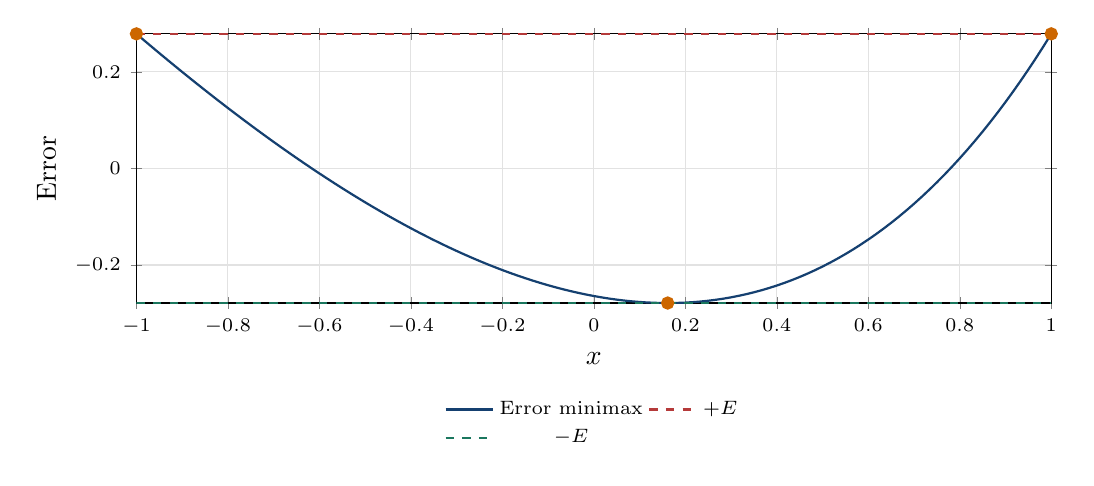
\begin{tikzpicture}\begin{axis}[base,axis lines=box,grid=major,minor tick num=0,width=13.2cm,height=5.0cm,xlabel={$x$},ylabel={Error},legend style={at={(0.5,-0.32)},anchor=north,legend columns=2,font=\scriptsize,draw=none,fill=white}]
\addplot[thick,azul,] coordinates {(-1,0.2788015858) (-0.9833333333,0.2653976027) (-0.9666666667,0.2520975281) (-0.95,0.2389031084) (-0.9333333333,0.2258161192) (-0.9166666667,0.2128383662) (-0.9,0.199971685) (-0.8833333333,0.1872179425) (-0.8666666667,0.1745790366) (-0.85,0.1620568975) (-0.8333333333,0.1496534875) (-0.8166666667,0.137370802) (-0.8,0.12521087) (-0.7833333333,0.1131757545) (-0.7666666667,0.1012675531) (-0.75,0.08948839895) (-0.7333333333,0.07784046074) (-0.7166666667,0.06632594376) (-0.7,0.05494709032) (-0.6833333333,0.04370618044) (-0.6666666667,0.03260553244) (-0.65,0.02164750361) (-0.6333333333,0.01083449085) (-0.6166666667,0.0001689313509) (-0.6,-0.01034669674) (-0.5833333333,-0.02070987362) (-0.5666666667,-0.03091803716) (-0.55,-0.04096858214) (-0.5333333333,-0.05085885957) (-0.5166666667,-0.06058617594) (-0.5,-0.07014779249) (-0.4833333333,-0.07954092439) (-0.4666666667,-0.08876274005) (-0.45,-0.09781036026) (-0.4333333333,-0.1066808574) (-0.4166666667,-0.1153712548) (-0.4,-0.1238785255) (-0.3833333333,-0.1321995919) (-0.3666666667,-0.1403313246) (-0.35,-0.1482705415) (-0.3333333333,-0.1560140072) (-0.3166666667,-0.1635584319) (-0.3,-0.1709004702) (-0.2833333333,-0.178036721) (-0.2666666667,-0.1849637257) (-0.25,-0.1916779675) (-0.2333333333,-0.1981758708) (-0.2166666667,-0.2044537997) (-0.2,-0.2105080572) (-0.1833333333,-0.2163348842) (-0.1666666667,-0.2219304585) (-0.15,-0.2272908935) (-0.1333333333,-0.2324122375) (-0.1166666667,-0.2372904721) (-0.1,-0.2419215116) (-0.08333333333,-0.2463012016) (-0.06666666667,-0.2504253177) (-0.05,-0.2542895648) (-0.03333333333,-0.2578895754) (-0.01666666667,-0.2612209086) (0,-0.264279049) (0.01666666667,-0.2670594052) (0.03333333333,-0.2695573086) (0.05,-0.2717680123) (0.06666666667,-0.2736866895) (0.08333333333,-0.2753084323) (0.1,-0.2766282503) (0.1166666667,-0.2776410693) (0.1333333333,-0.2783417297) (0.15,-0.2787249853) (0.1666666667,-0.2787855018) (0.1833333333,-0.2785178549) (0.2,-0.2779165296) (0.2166666667,-0.2769759179) (0.2333333333,-0.2756903176) (0.25,-0.2740539307) (0.2666666667,-0.2720608619) (0.2833333333,-0.2697051166) (0.3,-0.2669805995) (0.3166666667,-0.263881113) (0.3333333333,-0.2604003551) (0.35,-0.2565319182) (0.3666666667,-0.2522692867) (0.3833333333,-0.2476058357) (0.4,-0.2425348288) (0.4166666667,-0.2370494166) (0.4333333333,-0.2311426345) (0.45,-0.2248074007) (0.4666666667,-0.2180365145) (0.4833333333,-0.2108226542) (0.5,-0.2031583751) (0.5166666667,-0.1950361073) (0.5333333333,-0.1864481536) (0.55,-0.1773866877) (0.5666666667,-0.1678437514) (0.5833333333,-0.157811253) (0.6,-0.1472809648) (0.6166666667,-0.1362445208) (0.6333333333,-0.1246934144) (0.65,-0.1126189959) (0.6666666667,-0.1000124704) (0.6833333333,-0.08686489516) (0.7,-0.0731671771) (0.7166666667,-0.05891007034) (0.7333333333,-0.04408417361) (0.75,-0.02867992764) (0.7666666667,-0.01268761249) (0.7833333333,0.00390265511) (0.8,0.02110092456) (0.8166666667,0.03891741413) (0.8333333333,0.05736251384) (0.85,0.07644678831) (0.8666666667,0.09618097973) (0.8833333333,0.1165760108) (0.9,0.1376429879) (0.9166666667,0.1593932038) (0.9333333333,0.1818381414) (0.95,0.2049894763) (0.9666666667,0.2288590806) (0.9833333333,0.2534590256) (1,0.2788015858)};
\addlegendentry{Error minimax}
\addplot[thick,rojo,dashed] coordinates {(-1,0.2788015858) (1,0.2788015858)};
\addlegendentry{$+E$}
\addplot[thick,verde,dashed] coordinates {(-1,-0.2788015858) (1,-0.2788015858)};
\addlegendentry{$-E$}
\addplot[thick,orange!80!black,only marks,mark=*] coordinates {(-1,0.2788015858) (0.1614393616,-0.2788015858) (1,0.2788015858)};
\end{axis}\end{tikzpicture}
\caption{Alternancia del mejor aproximante lineal de $e^x$. Los dos bordes y un extremo interior alcanzan el mismo error en módulo.}\label{fig:cdf-11}\end{figure}

\section{Remez polinómico como intercambio de extremos}
Elegimos $m+2$ puntos alternantes iniciales. Resolvemos
\[
\sum_{j=0}^ma_jx_i^j+(-1)^iE=f(x_i),
\quad i=0,\ldots,m+1.
\]
Es un sistema lineal con $m+2$ incógnitas. Después calculamos extremos reales del error: bordes y raíces de $f'-p'$. Reemplazamos los puntos por una selección alternante de mayor amplitud y repetimos.

Una malla fina ayuda a localizar extremos, pero la certificación exige resolver o encerrar las raíces relevantes. Si la función presenta una oscilación estrecha, la malla puede omitir el peor extremo.

Usar Chebyshev como base mejora la escala del sistema. Un criterio de parada compara amplitudes máxima y mínima de los extremos activos y comprueba que ningún extremo omitido sea mayor. La convergencia práctica depende de la función y del procedimiento de intercambio; no todos los bucles improvisados heredan automáticamente el teorema ideal.

\section{Minimax ponderado y errores relativos}
Para un peso positivo continuo $\omega(x)$,
\[
\min_{p\in\mathcal P_m}\max_{[a,b]}|\omega(x)(f(x)-p(x))|.
\]
El sistema Remez es
\[
p(x_i)+(-1)^iE/\omega(x_i)=f(x_i).
\]
Si $f$ es positiva y queremos error relativo, elegimos $\omega=1/f$. Si $f$ se anula, el peso diverge; conviene factorizar el cero conocido. Para $\erf(x)$ cerca de cero, se aproxima $G(x^2)$ en vez de dividir un error por $\erf(0)=0$.

Para cola normal, aproximar el cociente de Mills y multiplicar por $\ph$ hace que el error relativo del cociente pase casi directamente a la cola, además del redondeo en el factor exponencial. Esta factorización adapta la optimización a la magnitud que interesa.

\section{Remez racional es un problema diferente}
Para $r=p/q$, la alternancia se refiere a $f-p/q$. Escribir
\[
f(x_i)q(x_i)-p(x_i)=(-1)^iE\,q(x_i)
\]
introduce productos entre el error desconocido $E$ y los coeficientes de $q$. El sistema no es lineal simultáneamente en todas las incógnitas. Congelar un denominador y resolver otro problema puede ser una etapa iterativa, pero no equivale a una solución exacta directa.

Además de extremos, debemos controlar polos y grados defectivos. La teoría de alternancia racional tiene condiciones adicionales sobre denominadores y grados efectivos. Usar el teorema polinómico cambiando una letra sería incorrecto.

Un método práctico puede partir de Padé, una aproximación Chebyshev o AAA, y luego mejorar error uniforme. La construcción y la certificación final se separan.

\section{Fracciones continuas y convergentes}
Una fracción continua generalizada es
\[
b_0+\cfrac{a_1}{b_1+\cfrac{a_2}{b_2+\cfrac{a_3}{b_3+\cdots}}}.
\]
Los convergentes $C_n=A_n/B_n$ se calculan con
\[
A_{-1}=1,\ A_0=b_0,\quad B_{-1}=0,\ B_0=1,
\]
\[
A_n=b_nA_{n-1}+a_nA_{n-2},\qquad
B_n=b_nB_{n-1}+a_nB_{n-2}.
\]
La identidad
\[
A_nB_{n-1}-A_{n-1}B_n
=(-1)^{n-1}\prod_{j=1}^na_j
\]
se prueba por inducción. Describe diferencias y, para ciertos signos, alternancia de convergentes.

Los numeradores y denominadores pueden crecer aunque el cociente sea moderado. Reescalar ambos pares conserva el cociente. El algoritmo Lentz evita formar directamente cantidades grandes y evalúa multiplicadores de actualización.

\section{Lentz modificado y qué garantiza la parada}
Para la fracción anterior, inicializamos $f=b_0$ (reemplazado por una cantidad pequeña no nula si es necesario), $C=f$, $D=0$. En cada paso,
\[
D\leftarrow b_n+a_nD,\quad C\leftarrow b_n+a_n/C,
\quad D\leftarrow1/D,\quad \Delta_n=CD,\quad f\leftarrow f\Delta_n.
\]
Si un denominador calculado es demasiado próximo a cero, se usa una protección escalada. Parar cuando $|\Delta_n-1|<\tau$ indica que el convergente apenas cambia.

Este criterio no es en general una cota matemática del resto. Una fracción puede converger lentamente o presentar cancelaciones que requieren límites de iteraciones y una ruta alternativa. En familias donde convergentes pares e impares encierran la respuesta, su diferencia sí puede ofrecer una cota, bajo las hipótesis de ese resultado.

\section{El puente entre ortogonalidad, Padé y medidas}
Sea una medida positiva $\mu$ y su transformada de Stieltjes
\[
S(z)=\int\frac{\dd\mu(t)}{z-t}
=\frac{\mu_0}z+\frac{\mu_1}{z^2}+\cdots,
\]
válida como expansión cuando el soporte es acotado y $z$ está suficientemente lejos, o como expansión asintótica con momentos apropiados. Una regla Gauss produce
\[
S_n(z)=\sum_{i=1}^n\frac{w_i}{z-x_i}.
\]
Al expandir cada denominador, los momentos coinciden hasta grado $2n-1$. Así $S_n$ es una aproximación de tipo Padé en infinito. Sus polos son los nodos de Gauss y sus residuos son pesos positivos.

La recurrencia de tres términos induce una fracción continua para la misma transformada. No son tres trucos desconectados: cuadratura, racionales y matrices de Jacobi codifican los mismos momentos de una medida.


\parte{VIII. La CDF normal: construir un evaluador completo}
\section{La región central y la serie alternante}
Expandiendo $\exp(-t^2/2)$ e integrando término a término en un intervalo compacto,
\[
\Phi(x)=\frac12+\frac1{\sqrt{2\pi}}
\sum_{k=0}^\infty\frac{(-1)^kx^{2k+1}}{2^kk!(2k+1)}.
\]
La justificación usa convergencia uniforme de la serie exponencial en todo compacto. Para $x<0$ se usa imparidad del término integral. Definamos magnitudes
\[
a_k=\frac{|x|^{2k+1}}{2^kk!(2k+1)},\qquad
\frac{a_{k+1}}{a_k}
=\frac{x^2(2k+1)}{2(k+1)(2k+3)}.
\]
Cuando las magnitudes restantes son decrecientes a cero, el error de truncamiento alternante es menor que el siguiente término. Si al principio crecen, no se usa la cota hasta entrar al tramo decreciente; la gran cancelación acumulada puede haber deteriorado ya el resultado.

En $x=1$, los términos dentro del factor $1/\sqrt{2\pi}$ son
\[
1-\frac16+\frac1{40}-\frac1{336}+\frac1{3456}-\cdots.
\]
Después del término $k=N$, la cota para la CDF es $a_{N+1}/\sqrt{2\pi}$. Sumar término a término mediante un cociente evita factoriales y potencias independientes.

\section{Una serie positiva derivada de una ecuación}
Sea $H(x)=e^{x^2/2}\int_0^xe^{-t^2/2}\dd t$. Diferenciando,
\[
H'(x)=1+xH(x),\qquad H(0)=0.
\]
Si $H=\sum_{k\ge0}h_kx^{2k+1}$, comparar coeficientes da
$h_0=1$ y $(2k+1)h_k=h_{k-1}$:
\[
H(x)=x+\frac{x^3}3+\frac{x^5}{15}+\frac{x^7}{105}+\cdots
=\sum_{k=0}^\infty\frac{x^{2k+1}}{(2k+1)!!}.
\]
Así,
\[
\Phi(x)=\frac12+\ph(x)H(x).
\]
Para $x\ge0$, los términos son positivos. El cociente es $x^2/(2k+3)$ y una cola geométrica se acota una vez que ese cociente es menor que uno. Si sumamos hasta $N$ y $r=x^2/(2N+5)<1$,
\[
\sum_{k=N+1}^\infty\frac{x^{2k+1}}{(2k+1)!!}
\le\frac{x^{2N+3}}{(2N+3)!!}\frac1{1-r}.
\]
El cociente disminuye en los términos siguientes.

La serie evita cancelación central, pero $H$ crece como $e^{x^2/2}$ y puede desbordar en cola. Multiplicar luego por $\ph$ no arregla un infinito intermedio. Es una representación regional.

\section{Cuadratura central y comparación de esfuerzos}
Para $x>0$,
\[
\Phi(x)=\frac12+\frac{x}{2\sqrt{2\pi}}
\int_{-1}^1
\exp\left[-\frac{x^2(s+1)^2}{8}\right]\dd s.
\]
Una regla Legendre de $n$ nodos produce una suma positiva y suave. La cota gaussiana involucra la derivada de orden $2n$ de la función transformada, con factores de escala $x/2$.

En una región acotada, una regla pequeña puede ser precisa. Al crecer $x$, el integrando se concentra cerca de $s=-1$ y la escala cambia. Aumentar $n$ o dividir el dominio ayuda, pero una fórmula directa de cola puede ser mucho más eficiente.

Una comparación honesta registra evaluaciones de exponenciales, preparación de nodos y error de referencia. La exactitud hasta grado $2n-1$ no dice cuántos dígitos obtendremos sin información sobre la función.






\begin{figure}[htbp]\centering
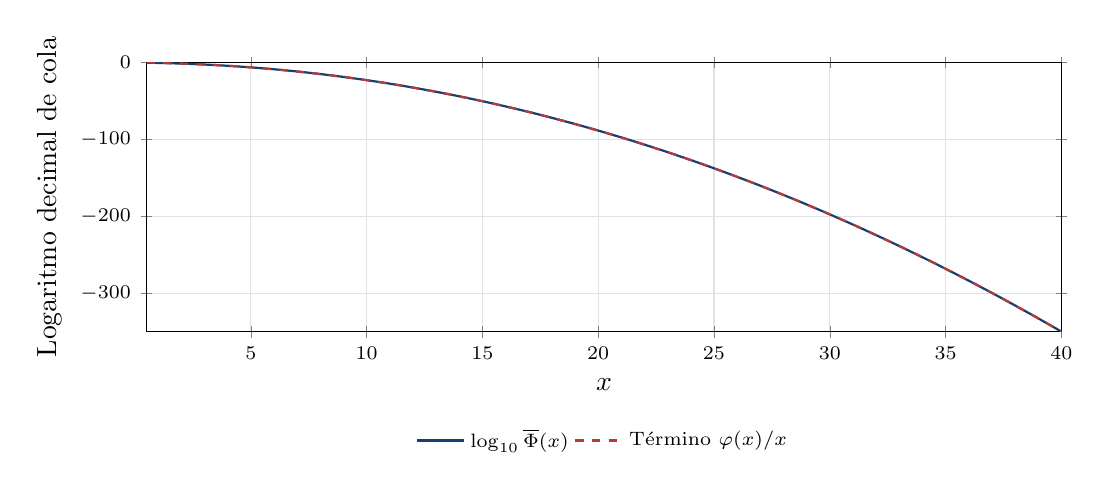
\begin{tikzpicture}\begin{axis}[base,axis lines=box,grid=major,minor tick num=0,width=13.2cm,height=5.0cm,xlabel={$x$},ylabel={Logaritmo decimal de cola},legend style={at={(0.5,-0.32)},anchor=north,legend columns=2,font=\scriptsize,draw=none,fill=white}]
\addplot[thick,azul,] coordinates {(0.5,-0.5106919893) (0.8291666667,-0.6914248049) (1.158333333,-0.9088114984) (1.4875,-1.164681105) (1.816666667,-1.46049629) (2.145833333,-1.797426165) (2.475,-2.176407837) (2.804166667,-2.598196197) (3.133333333,-3.063403222) (3.4625,-3.572528567) (3.791666667,-4.125983244) (4.120833333,-4.724107918) (4.45,-5.367187069) (4.779166667,-6.055459991) (5.108333333,-6.789129384) (5.4375,-7.568368099) (5.766666667,-8.393324473) (6.095833333,-9.264126569) (6.425,-10.18088558) (6.754166667,-11.14369856) (7.083333333,-12.15265065) (7.4125,-13.20781691) (7.741666667,-14.30926377) (8.070833333,-15.45705033) (8.4,-16.65122931) (8.729166667,-17.89184796) (9.058333333,-19.17894876) (9.3875,-20.51257002) (9.716666667,-21.89274644) (10.04583333,-23.31950947) (10.375,-24.79288777) (10.70416667,-26.31290748) (11.03333333,-27.87959251) (11.3625,-29.49296481) (11.69166667,-31.15304453) (12.02083333,-32.85985026) (12.35,-34.61339913) (12.67916667,-36.41370702) (13.00833333,-38.2607886) (13.3375,-40.15465754) (13.66666667,-42.09532651) (13.99583333,-44.08280735) (14.325,-46.11711106) (14.65416667,-48.19824797) (14.98333333,-50.3262277) (15.3125,-52.50105929) (15.64166667,-54.72275122) (15.97083333,-56.99131145) (16.3,-59.30674748) (16.62916667,-61.66906634) (16.95833333,-64.07827471) (17.2875,-66.53437884) (17.61666667,-69.03738468) (17.94583333,-71.58729784) (18.275,-74.18412362) (18.60416667,-76.82786706) (18.93333333,-79.51853294) (19.2625,-82.25612578) (19.59166667,-85.04064991) (19.92083333,-87.8721094) (20.25,-90.75050817) (20.57916667,-93.67584992) (20.90833333,-96.6481382) (21.2375,-99.66737639) (21.56666667,-102.7335677) (21.89583333,-105.8467152) (22.225,-109.0068219) (22.55416667,-112.2138906) (22.88333333,-115.4679239) (23.2125,-118.7689245) (23.54166667,-122.1168948) (23.87083333,-125.5118371) (24.2,-128.9537539) (24.52916667,-132.4426473) (24.85833333,-135.9785193) (25.1875,-139.5613719) (25.51666667,-143.1912073) (25.84583333,-146.868027) (26.175,-150.5918331) (26.50416667,-154.3626272) (26.83333333,-158.180411) (27.1625,-162.0451861) (27.49166667,-165.956954) (27.82083333,-169.9157162) (28.15,-173.9214742) (28.47916667,-177.9742294) (28.80833333,-182.0739831) (29.1375,-186.2207366) (29.46666667,-190.4144912) (29.79583333,-194.655248) (30.125,-198.9430083) (30.45416667,-203.2777732) (30.78333333,-207.6595438) (31.1125,-212.0883212) (31.44166667,-216.5641063) (31.77083333,-221.0869003) (32.1,-225.656704) (32.42916667,-230.2735184) (32.75833333,-234.9373444) (33.0875,-239.6481829) (33.41666667,-244.4060348) (33.74583333,-249.2109009) (34.075,-254.062782) (34.40416667,-258.9616788) (34.73333333,-263.9075922) (35.0625,-268.9005229) (35.39166667,-273.9404717) (35.72083333,-279.0274391) (36.05,-284.1614259) (36.37916667,-289.3424329) (36.70833333,-294.5704605) (37.0375,-299.8455094) (37.36666667,-305.1675804) (37.69583333,-310.5366738) (38.025,-315.9527904) (38.35416667,-321.4159307) (38.68333333,-326.9260952) (39.0125,-332.4832846) (39.34166667,-338.0874992) (39.67083333,-343.7387397) (40,-349.4370065)};
\addlegendentry{$\log_{10}\overline\Phi(x)$}
\addplot[thick,rojo,dashed] coordinates {(0.5,-0.1523467488) (0.8291666667,-0.4670242669) (1.158333333,-0.754277783) (1.4875,-1.052019108) (1.816666667,-1.375011396) (2.145833333,-1.730562258) (2.475,-2.122827705) (2.804166667,-2.554398665) (3.133333333,-3.02699989) (3.4625,-3.54183763) (3.791666667,-4.099788665) (4.120833333,-4.701510339) (4.45,-5.347508184) (4.779166667,-6.038179342) (5.108333333,-6.773841495) (5.4375,-7.554752746) (5.766666667,-8.381125643) (6.095833333,-9.253137306) (6.425,-10.17093689) (6.754166667,-11.13465118) (7.083333333,-12.14438884) (7.4125,-13.20024372) (7.741666667,-14.30229746) (8.070833333,-15.45062145) (8.4,-16.64527854) (8.729166667,-17.88632434) (9.058333333,-19.17380826) (9.3875,-20.50777442) (9.716666667,-21.8882624) (10.04583333,-23.3153078) (10.375,-24.78894277) (10.70416667,-26.30919648) (11.03333333,-27.87609541) (11.3625,-29.48966374) (11.69166667,-31.14992354) (12.02083333,-32.85689508) (12.35,-34.61059695) (12.67916667,-36.4110463) (13.00833333,-38.25825896) (13.3375,-40.15224955) (13.66666667,-42.09303165) (13.99583333,-44.08061785) (14.325,-46.11501986) (14.65416667,-48.19624861) (14.98333333,-50.32431429) (15.3125,-52.49922642) (15.64166667,-54.72099392) (15.97083333,-56.98962516) (16.3,-59.30512799) (16.62916667,-61.66750977) (16.95833333,-64.07677747) (17.2875,-66.53293762) (17.61666667,-69.03599639) (17.94583333,-71.58595963) (18.275,-74.18283283) (18.60416667,-76.82662123) (18.93333333,-79.51732975) (19.2625,-82.2549631) (19.59166667,-85.03952572) (19.92083333,-87.87102183) (20.25,-90.74945545) (20.57916667,-93.67483042) (20.90833333,-96.64715037) (21.2375,-99.66641878) (21.56666667,-102.7326389) (21.89583333,-105.845814) (22.225,-109.0059471) (22.55416667,-112.213041) (22.88333333,-115.4670984) (23.2125,-118.7681221) (23.54166667,-122.1161146) (23.87083333,-125.5110783) (24.2,-128.9530155) (24.52916667,-132.4419284) (24.85833333,-135.9778193) (25.1875,-139.5606901) (25.51666667,-143.1905428) (25.84583333,-146.8673793) (26.175,-150.5912015) (26.50416667,-154.3620112) (26.83333333,-158.1798099) (27.1625,-162.0445994) (27.49166667,-165.9563812) (27.82083333,-169.9151569) (28.15,-173.9209279) (28.47916667,-177.9736956) (28.80833333,-182.0734614) (29.1375,-186.2202265) (29.46666667,-190.4139924) (29.79583333,-194.6547602) (30.125,-198.9425311) (30.45416667,-203.2773062) (30.78333333,-207.6590867) (31.1125,-212.0878737) (31.44166667,-216.5636681) (31.77083333,-221.0864711) (32.1,-225.6562835) (32.42916667,-230.2731064) (32.75833333,-234.9369406) (33.0875,-239.6477871) (33.41666667,-244.4056468) (33.74583333,-249.2105203) (34.075,-254.0624087) (34.40416667,-258.9613127) (34.73333333,-263.907233) (35.0625,-268.9001704) (35.39166667,-273.9401256) (35.72083333,-279.0270994) (36.05,-284.1610924) (36.37916667,-289.3421053) (36.70833333,-294.5701388) (37.0375,-299.8451934) (37.36666667,-305.1672699) (37.69583333,-310.5363687) (38.025,-315.9524906) (38.35416667,-321.415636) (38.68333333,-326.9258055) (39.0125,-332.4829997) (39.34166667,-338.0872191) (39.67083333,-343.7384642) (40,-349.4367354)};
\addlegendentry{Término $\varphi(x)/x$}
\end{axis}\end{tikzpicture}
\caption{La cola normal recorre cientos de órdenes de magnitud. Graficar su logaritmo conserva información que una escala de probabilidades ordinarias perdería.}\label{fig:cdf-13}\end{figure}

\section{El cociente de Mills y una integral positiva}
Definamos $R(x)=\Q(x)/\ph(x)$ para $x\ge0$. En la cola sustituimos $t=x+s$:
\[
\Q(x)=\ph(x)\int_0^\infty e^{-xs-s^2/2}\dd s,
\qquad R(x)=\int_0^\infty e^{-xs-s^2/2}\dd s.
\]
Ahora la cantidad integrada tiene tamaño $1/x$ en cola y no contiene el factor extremadamente pequeño $\ph(x)$. Para $x>0$, con $u=xs$,
\[
R(x)=\frac1x\int_0^\infty e^{-u}
\exp\left(-\frac{u^2}{2x^2}\right)\dd u.
\]
Esta representación invita a Gauss--Laguerre estándar. El factor no ponderado tiende uniformemente en compactos a uno y la medida $e^{-u}$ ya maneja el infinito.

La CDF pequeña se reconstruye con $\log\Q=-x^2/2-\log(2\pi)/2+\log R(x)$. El logaritmo sigue representable incluso cuando $\Q$ no cabe en binary64.

\section{Cotas de Mills por integración por partes}
Como $\ph'=-t\ph$, para $x>0$,
\[
\Q(x)=\int_x^\infty\frac1t\,t\ph(t)\dd t
=\frac{\ph(x)}x-\int_x^\infty\frac{\ph(t)}{t^2}\dd t.
\]
El último término es positivo, así que $\Q<\ph/x$. También
$\int_x^\infty\ph(t)/t^2\dd t\le\Q(x)/x^2$, de donde
\[
\frac{x}{x^2+1}\ph(x)\le\Q(x)<\frac{\ph(x)}x.
\]
Las desigualdades son estrictas para $x>0$ en los pasos no degenerados.

La anchura relativa del intervalo es del orden de $1/x^2$. Es una certificación rápida pero no alcanza precisión completa para un $x$ moderado. Sirve para elegir cortes de dominio y verificar resultados de métodos más elaborados.

\section{Expansión asintótica de cola y resto con signo}
Definamos $J_m(x)=\int_x^\infty t^{-2m}\ph(t)\dd t$. Integración por partes da
\[
J_m(x)=\frac{\ph(x)}{x^{2m+1}}-(2m+1)J_{m+1}(x).
\]
Iterando desde $J_0=\Q$,
\[
\Q(x)=\ph(x)\sum_{k=0}^{N-1}
\frac{(-1)^k(2k-1)!!}{x^{2k+1}}
+(-1)^N(2N-1)!!J_N(x),
\]
con $(-1)!!=1$. Como $J_N<\ph(x)/x^{2N+1}$,
\[
|R_N^{\rm cola}|<
\ph(x)\frac{(2N-1)!!}{x^{2N+1}}.
\]
El signo del resto permite encerrar la cola con truncaciones consecutivas.

Para $x$ fijo, las magnitudes de términos tienen cociente $(2k+1)/x^2$ y eventualmente crecen. La expansión es asintótica, no una serie convergente. La truncación óptima suele estar cerca del menor término; agregar infinitamente términos empeora. Para $x$ moderado, la cota mínima puede no alcanzar la tolerancia solicitada: hay que cambiar de método.






\begin{figure}[htbp]\centering
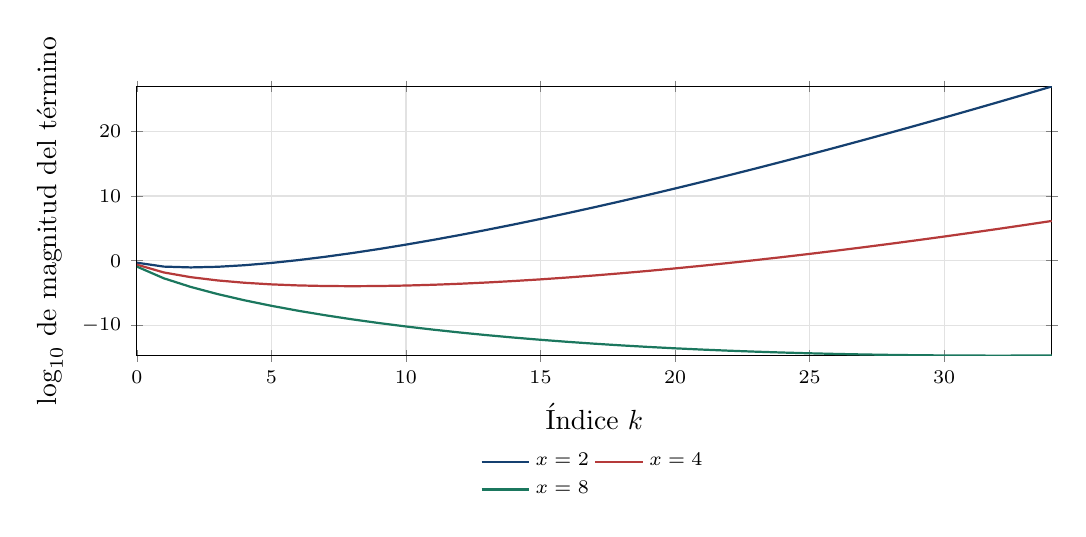
\begin{tikzpicture}\begin{axis}[base,axis lines=box,grid=major,minor tick num=0,width=13.2cm,height=5.0cm,xlabel={Índice $k$},ylabel={$\log_{10}$ de magnitud del término},legend style={at={(0.5,-0.32)},anchor=north,legend columns=2,font=\scriptsize,draw=none,fill=white}]
\addplot[thick,azul,] coordinates {(0,-0.3010299957) (1,-0.903089987) (2,-1.028028724) (3,-0.9311187106) (4,-0.6880806619) (5,-0.3358981438) (6,0.10343455) (7,0.615317911) (8,1.189349179) (9,1.817738109) (10,2.494431718) (11,3.214591022) (12,3.974258867) (13,4.770138884) (14,5.599442657) (15,6.459780663) (16,7.349082366) (17,8.265536314) (18,9.207544367) (19,10.1736861) (20,11.16269072) (21,12.17341458) (22,13.20482305) (23,14.25597557) (24,15.32601343) (25,16.41414952) (26,17.51965971) (27,18.64187559) (28,19.78017828) (29,20.93399315) (30,22.10278517) (31,23.28605501) (32,24.48333557) (33,25.69418894) (34,26.91820375)};
\addlegendentry{$x=2$}
\addplot[thick,rojo,] coordinates {(0,-0.6020599913) (1,-1.806179974) (2,-2.533178702) (3,-3.03832868) (4,-3.397350623) (5,-3.647228096) (6,-3.809955394) (7,-3.900132024) (8,-3.928160748) (9,-3.901831809) (10,-3.827198191) (11,-3.709098878) (12,-3.551491025) (13,-3.357670999) (14,-3.130427218) (15,-2.872149202) (16,-2.584907491) (17,-2.270513534) (18,-1.930565472) (19,-1.566483731) (20,-1.179539106) (21,-0.7708752324) (22,-0.3415267595) (23,0.1075657717) (24,0.5755436469) (25,1.061619744) (26,1.565069938) (27,2.085225825) (28,2.621468532) (29,3.173223405) (30,3.739955434) (31,4.321165286) (32,4.916385853) (33,5.525179227) (34,6.147134047)};
\addlegendentry{$x=4$}
\addplot[thick,verde,] coordinates {(0,-0.903089987) (1,-2.709269961) (2,-4.03832868) (3,-5.14553865) (4,-6.106620584) (5,-6.958558048) (6,-7.723345337) (7,-8.415581959) (8,-9.045670674) (9,-9.621401726) (10,-10.1488281) (11,-10.63278878) (12,-11.07724092) (13,-11.48548088) (14,-11.86029709) (15,-12.20407907) (16,-12.51889735) (17,-12.80656338) (18,-13.06867531) (19,-13.30665356) (20,-13.52176893) (21,-13.71516505) (22,-13.88787656) (23,-14.04084402) (24,-14.17492614) (25,-14.29091003) (26,-14.38951983) (27,-14.47142394) (28,-14.53724122) (29,-14.58754634) (30,-14.6228743) (31,-14.64372444) (32,-14.65056387) (33,-14.64383048) (34,-14.62393565)};
\addlegendentry{$x=8$}
\end{axis}\end{tikzpicture}
\caption{Magnitudes de términos asintóticos de Mills. Cada curva primero decrece y luego crece: el punto bajo sugiere truncación, no convergencia de la serie infinita.}\label{fig:cdf-14}\end{figure}

\section{Fracción continua normal desde integrales auxiliares}
Definamos
\[
I_n(x)=\int_0^\infty s^n e^{-xs-s^2/2}\dd s.
\]
Para $n=0$, integrar la derivada del exponencial da $xI_0+I_1=1$. Para $n\ge1$, integrar la derivada de $s^ne^{-xs-s^2/2}$ da
\[
nI_{n-1}=xI_n+I_{n+1}.
\]
Con $r_n=I_n/I_{n-1}>0$, $r_n=n/(x+r_{n+1})$. Por tanto
\[
R(x)=\cfrac1{x+\cfrac1{x+\cfrac2{x+\cfrac3{x+\cdots}}}},
\qquad x>0.
\]
La derivación introduce colas positivas de la fracción; la convergencia corresponde a esta familia de Stieltjes.

La primera truncación es $1/x$, cota superior, y la siguiente $x/(x^2+1)$, cota inferior. Los convergentes sucesivos alternan y pueden proporcionar un intervalo, con la teoría de esta fracción. En $x=0$, las truncaciones con denominadores cero requieren otro esquema: no basta aplicar la misma fórmula flotante.

\section{Una interpretación Stieltjes del cociente}
Sea $Z\sim N(0,1)$ y $x>0$. Usando una representación Laplace de $1/(x^2+t^2)$,
\[
\E\left[\frac{x^2}{x^2+Z^2}\right]
=\int_0^\infty e^{-u}
\left(1+\frac{2u}{x^2}\right)^{-1/2}\dd u.
\]
Evaluando mediante un cambio de variable o la integral gaussiana se obtiene
\[
xR(x)=\E\left[\frac1{1+Z^2/x^2}\right].
\]
Esta expresión es una transformada de Stieltjes de la medida de $Z^2$. Sus momentos son $\E Z^{2k}=(2k-1)!!$, que explican los coeficientes de la expansión asintótica.

Al aproximar esa medida con una regla Gauss positiva se obtiene un racional con polos fuera de $s=1/x^2\ge0$. Esta estructura favorece estabilidad y conecta otra vez normal, Padé, ortogonalidad y cuadratura.

\section{Función error escalada y reconstrucción estable}
Para $z\ge0$,
\[
\erfcx(z)=e^{z^2}\erfc(z),\qquad
\Q(x)=\frac12e^{-x^2/2}\erfcx(x/\sqrt2).
\]
La función escalada evita el subdesbordamiento temprano. Su expansión es
\[
\erfcx(z)\sim\frac1{\sqrt\pi z}
\left(1-\frac1{2z^2}+\frac3{4z^4}-\cdots\right).
\]
Para devolver logaritmo,
\[
\log\Q(x)=-\frac{x^2}2-\log2+\log\erfcx(x/\sqrt2).
\]
Para $x<0$ usamos simetría y una operación estable de complemento. Si calculamos $s=\Q(|x|)$, entonces
\[
\Phi(x)=
\begin{cases}s,&x<0,\\1-s,&x\ge0.\end{cases}
\]
Si se solicita una cola pequeña, se devuelve $s$ directamente. No se obtiene restando una salida que ya redondeó a uno.

\section{Por regiones: diseño de un evaluador}
Un esquema educativo puede usar:
\begin{enumerate}
\item Simetría para reducir a $x\ge0$ y recordar qué cola se solicita.
\item Una serie o aproximación racional central para $0\le x\le A$.
\item Una fracción continua, cuadratura de Mills o racional escalado para $A<x<B$.
\item Expansión asintótica con cota de resto cuando $x\ge B$ y satisface la tolerancia.
\item Reconstrucción en escala logarítmica cuando la cola no es representable.
\end{enumerate}
Los valores $A,B$ no son constantes matemáticas universales. Se eligen después de medir errores y costos del método concreto, incluida la precisión.

En cada frontera se prueban puntos de ambos lados, continuidad numérica, monotonía y complementariedad. La aritmética puede hacer que una CDF redondee exactamente a uno; esto es compatible con devolver una supervivencia positiva por una ruta independiente.

\section{Cody y la arquitectura de bibliotecas actuales}
El trabajo de Cody de 1969 construye aproximaciones racionales de la función error en regiones. La documentación consultada de R atribuye su evaluador de CDF normal a la familia SPECFUN de Cody y su cuantil a AS 241 de Wichura, con desarrollos posteriores para colas logarítmicas.

Estas referencias distinguen dos funciones: evaluar $\Phi(x)$ y resolver $\Phi(x)=p$. No se describe AS 241 como una fórmula para la CDF directa. Tampoco se copian aquí tablas de coeficientes como si se hubieran deducido simbólicamente: los coeficientes de un minimax se obtienen por una optimización numérica más una validación.

La lección reproducible es la estructura: simetría, región, función escalada, polinomios/racionales de bajo grado, tratamiento explícito de colas y pruebas en frontera.

\section{Probabilidades entre dos valores}
Para $a<b$,
\[
\Pr(a<Z\le b)=\Phi(b)-\Phi(a).
\]
Si ambos están en la cola derecha, conviene $\Q(a)-\Q(b)$. Si $\ell_a=\log\Q(a)$ y $\ell_b=\log\Q(b)$ con $\ell_b<\ell_a$,
\[
\log\Pr(a<Z\le b)
=\ell_a+\log(1-e^{\ell_b-\ell_a}).
\]
La segunda operación se evalúa con la fórmula estable de complemento logarítmico.

Para un intervalo muy corto, $b=a+h$,
\[
\int_a^{a+h}\ph(t)\dd t
=\ph(a)\left[h-\frac a2h^2+\frac{a^2-1}{6}h^3+\cdots\right].
\]
Se deduce expandiendo la densidad, no restando CDF cercanas. La cota del resto requiere derivadas en el intervalo; si $|a|h$ es grande, la expansión local pierde ventaja.

\section{Derivadas respecto de media, escala y argumento}
Para $F(x;\mu,\sigma)=\Phi(z)$, $z=(x-\mu)/\sigma$,
\[
\frac{\partial F}{\partial x}=\frac{\ph(z)}\sigma,\quad
\frac{\partial F}{\partial\mu}=-\frac{\ph(z)}\sigma,\quad
\frac{\partial F}{\partial\sigma}=-\frac{z\ph(z)}\sigma.
\]
Si trabajamos con la cola superior,
$\partial_x\log S=-\ph(z)/[\sigma\Q(z)]$.
La densidad puede subdesbordar mientras el cociente de Mills permite calcular esa razón.

Derivar un aproximante no garantiza que la derivada aproxime bien a la derivada exacta. Una cota uniforme de valores no implica una cota uniforme de derivadas sin condiciones adicionales. Las aplicaciones de optimización necesitan validar ambas salidas.

\section{Cómo verificar una CDF normal}
Comprobaciones estructurales:
\[
\Phi(0)=1/2,\quad \Phi(-x)=\Q(x),\quad
\Phi(x)+\Q(x)=1,\quad \Phi'\!=\ph>0.
\]
En cola verificamos cotas de Mills y, donde sea aplicable, un intervalo asintótico o de convergentes. Se comparan rutas independientes: serie, cuadratura y aritmética de precisión ampliada.

Una tolerancia relativa en la cola se mide sobre $\Q$, no sobre $\Phi$. Un error en logaritmo se registra como $|\widehat\ell-\ell|$. Para probabilidades menores que el mínimo representable, devolver cero con logaritmo finito es una política explícita; no se afirma error relativo pequeño sobre un cero redondeado.

Los ejemplos tabulados al final incluyen centro, colas moderadas, colas extremas e intervalos estrechos para mostrar estos cambios de escala.


\parte{IX. Gamma incompleta: series, fracciones y transición}
\section{La función gamma y sus escalas}
La identidad $\Gamma(a+1)=a\Gamma(a)$ permite mover parámetros positivos. Para $a$ grande, $\Gamma(a)$ supera pronto el rango flotante aunque una probabilidad regularizada esté entre cero y uno. Por eso se calcula
\[
L=\log\Gamma(a),\qquad
D(a,x)=\exp[a\log x-x-\log\Gamma(a)].
\]
El factor $D$ aparece en las series y fracciones de gamma incompleta. La normalización se hace antes de formar números enormes.

La fórmula de Stirling es
\[
\log\Gamma(a)\sim
\left(a-\frac12\right)\log a-a+\frac12\log(2\pi)
+\frac1{12a}-\frac1{360a^3}+\cdots.
\]
Es una expansión asintótica; no se debe sumar infinitamente para un $a$ fijo. Una deducción de su término principal se obtiene por Laplace alrededor del máximo de $(a-1)\log t-t$, con una escala de fluctuación de orden $\sqrt a$. Los coeficientes posteriores se deducen expandiendo la fase y los momentos gaussianos, o con Euler--Maclaurin.

Cerca de uno, un evaluador log-gamma especializado evita pérdidas por recurrencias y cancelación. Las implementaciones de Lanczos o Spouge usan aproximaciones de esta función; construirlas y certificar coeficientes constituye otro problema de aproximación racional/exponencial.

\section{Normalización y recurrencias exactas}
Definimos
\[
\gamma(a,x)=\int_0^x t^{a-1}e^{-t}\dd t,\qquad
\Gamma(a,x)=\int_x^\infty t^{a-1}e^{-t}\dd t,
\]
\[
P(a,x)=\frac{\gamma(a,x)}{\Gamma(a)},\qquad
Q(a,x)=\frac{\Gamma(a,x)}{\Gamma(a)},\qquad P+Q=1.
\]
Aquí $\Gamma(a)$ completa y $\Gamma(a,x)$ incompleta comparten símbolo, pero el número de argumentos distingue su significado.

Integración por partes da
\[
\gamma(a+1,x)=a\gamma(a,x)-x^ae^{-x},
\quad
\Gamma(a+1,x)=a\Gamma(a,x)+x^ae^{-x}.
\]
Regularizando,
\[
P(a+1,x)=P(a,x)-\frac{x^ae^{-x}}{\Gamma(a+1)},\quad
Q(a+1,x)=Q(a,x)+\frac{x^ae^{-x}}{\Gamma(a+1)}.
\]
En la primera hay resta; en la segunda, suma positiva. Según la región y la cola deseada, una dirección de recurrencia puede ser estable y otra perder cifras.






\begin{figure}[htbp]\centering
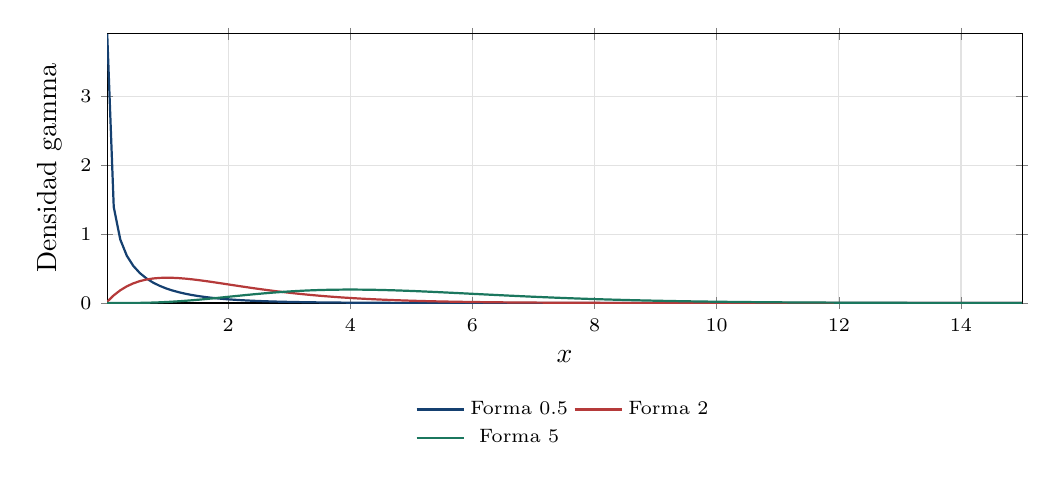
\begin{tikzpicture}\begin{axis}[base,axis lines=box,grid=major,minor tick num=0,width=13.2cm,height=5.0cm,xlabel={$x$},ylabel={Densidad gamma},legend style={at={(0.5,-0.32)},anchor=north,legend columns=2,font=\scriptsize,draw=none,fill=white}]
\addplot[thick,azul,] coordinates {(0.02,3.91042694) (0.127,1.394337167) (0.234,0.9229798635) (0.341,0.6869948095) (0.448,0.538545162) (0.555,0.4347555498) (0.662,0.3576787358) (0.769,0.2981875022) (0.876,0.2510331319) (0.983,0.2129299877) (1.09,0.1816899182) (1.197,0.1557856654) (1.304,0.1341115752) (1.411,0.1158435993) (1.518,0.1003529525) (1.625,0.08715049294) (1.732,0.07584956198) (1.839,0.06614037407) (1.946,0.0577718911) (2.053,0.05053869432) (2.16,0.0442712829) (2.267,0.03882877713) (2.374,0.03409334445) (2.481,0.02996588248) (2.588,0.0263626345) (2.695,0.02321250713) (2.802,0.02045492351) (2.909,0.01803809024) (3.016,0.0159175872) (3.123,0.01405521213) (3.23,0.01241802775) (3.337,0.01097757149) (3.444,0.009709196632) (3.551,0.008591520333) (3.658,0.00760595932) (3.765,0.006736337674) (3.872,0.005968554384) (3.979,0.00529030061) (4.086,0.004690818502) (4.193,0.004160694893) (4.3,0.003691684377) (4.407,0.00327655722) (4.514,0.002908968343) (4.621,0.002583344223) (4.728,0.002294785089) (4.835,0.002038980181) (4.942,0.001812134228) (5.049,0.001610903552) (5.156,0.001432340463) (5.263,0.001273844805) (5.37,0.00113312169) (5.477,0.001008144571) (5.584,0.0008971229604) (5.691,0.000798474175) (5.798,0.0007107985809) (5.905,0.0006328578872) (6.012,0.0005635560967) (6.119,0.0005019227748) (6.226,0.0004470983439) (6.333,0.0003983211487) (6.44,0.0003549160721) (6.547,0.000316284508) (6.654,0.0002818955258) (6.761,0.0002512780792) (6.868,0.000224014133) (6.975,0.0001997325958) (7.082,0.0001781039624) (7.189,0.0001588355793) (7.296,0.0001416674612) (7.403,0.0001263685899) (7.51,0.0001127336416) (7.617,0.0001005800894) (7.724,8.974563874e-05) (7.831,8.008595594e-05) (7.938,7.147265563e-05) (8.045,6.379151736e-05) (8.152,5.694090451e-05) (8.259,5.083036222e-05) (8.366,4.537937372e-05) (8.473,4.051625682e-05) (8.58,3.617718452e-05) (8.687,3.230531563e-05) (8.794,2.88500227e-05) (8.901,2.57662063e-05) (9.008,2.301368593e-05) (9.115,2.055665866e-05) (9.222,1.836321811e-05) (9.329,1.640492675e-05) (9.436,1.465643568e-05) (9.543,1.309514649e-05) (9.65,1.170091048e-05) (9.757,1.045576109e-05) (9.864,9.343675825e-06) (9.971,8.350364371e-06) (10.078,7.463080017e-06) (10.185,6.670451776e-06) (10.292,5.96233491e-06) (10.399,5.329677827e-06) (10.506,4.764403539e-06) (10.613,4.259304068e-06) (10.72,3.807946385e-06) (10.827,3.404588593e-06) (10.934,3.044105248e-06) (11.041,2.721920798e-06) (11.148,2.433950263e-06) (11.255,2.176546351e-06) (11.362,1.946452311e-06) (11.469,1.740759902e-06) (11.576,1.556871907e-06) (11.683,1.392468704e-06) (11.79,1.245478456e-06) (11.897,1.11405051e-06) (12.004,9.965316798e-07) (12.111,8.914450777e-07) (12.218,7.974712285e-07) (12.325,7.134312199e-07) (12.432,6.382716633e-07) (12.539,5.710512728e-07) (12.646,5.10928886e-07) (12.753,4.571527705e-07) (12.86,4.090510785e-07) (12.967,3.660233246e-07) (13.074,3.275327766e-07) (13.181,2.93099662e-07) (13.288,2.622951005e-07) (13.395,2.347356864e-07) (13.502,2.100786496e-07) (13.609,1.880175341e-07) (13.716,1.682783371e-07) (13.823,1.506160613e-07) (13.93,1.34811634e-07) (14.037,1.206691549e-07) (14.144,1.080134375e-07) (14.251,9.66878119e-08) (14.358,8.655216147e-08) (14.465,7.748116889e-08) (14.572,6.936274823e-08) (14.679,6.209664387e-08) (14.786,5.559317825e-08) (14.893,4.977213265e-08) (15,4.456174669e-08)};
\addlegendentry{Forma $0.5$}
\addplot[thick,rojo,] coordinates {(0.02,0.01960397347) (0.127,0.1118531764) (0.234,0.1851786649) (0.341,0.2424710877) (0.448,0.2862292984) (0.555,0.318610105) (0.662,0.3414719561) (0.769,0.3564132847) (0.876,0.3648061406) (0.983,0.3678256763) (1.09,0.3664759781) (1.197,0.3616126841) (1.304,0.3539627715) (1.411,0.3441418585) (1.518,0.3326693181) (1.625,0.3199814722) (1.732,0.3064430986) (1.839,0.2923574579) (1.946,0.2779750226) (2.053,0.2635010669) (2.16,0.2491022614) (2.267,0.2349123934) (2.374,0.2210373242) (2.481,0.2075592796) (2.588,0.194540556) (2.695,0.1820267189) (2.802,0.1700493564) (2.909,0.1586284473) (3.016,0.1477743915) (3.123,0.1374897484) (3.23,0.1277707211) (3.337,0.11860842) (3.444,0.1099899354) (3.551,0.1018992452) (3.658,0.094317979) (3.765,0.08722606007) (3.872,0.08060224062) (3.979,0.07442454627) (4.086,0.06867064226) (4.193,0.06331813286) (4.3,0.05834480375) (4.407,0.05372881581) (4.514,0.04944885768) (4.621,0.04548426359) (4.728,0.0418151017) (4.835,0.03842223805) (4.942,0.03528737977) (5.049,0.03239310148) (5.156,0.02972285754) (5.263,0.02726098299) (5.37,0.02499268514) (5.477,0.02290402787) (5.584,0.02098191014) (5.691,0.01921403994) (5.798,0.01758890507) (5.905,0.01609574142) (6.012,0.01472449967) (6.119,0.01346581112) (6.226,0.01231095296) (6.333,0.01125181373) (6.44,0.01028085902) (6.547,0.009391097898) (6.654,0.008576050189) (6.761,0.007829714814) (6.868,0.007146539275) (6.975,0.006521390413) (7.082,0.005949526477) (7.189,0.005426570545) (7.296,0.00494848531) (7.403,0.004511549221) (7.51,0.004112333976) (7.617,0.00374768333) (7.724,0.003414693178) (7.831,0.003110692887) (7.938,0.002833227818) (8.045,0.002580042984) (8.152,0.002349067815) (8.259,0.002138401942) (8.366,0.001946301981) (8.473,0.00177116924) (8.58,0.001611538306) (8.687,0.001466066456) (8.794,0.00133352385) (8.901,0.001212784444) (9.008,0.00110281759) (9.115,0.001002680273) (9.222,0.0009115099332) (9.329,0.0008285178536) (9.436,0.0007529830514) (9.543,0.000684246655) (9.65,0.0006217067219) (9.757,0.0005648134695) (9.864,0.0005130648877) (9.971,0.0004660027045) (10.078,0.0004232086789) (10.185,0.0003843011952) (10.292,0.0003489321366) (10.399,0.0003167840165) (10.506,0.0002875673462) (10.613,0.0002610182225) (10.72,0.0002368961155) (10.827,0.0002149818428) (10.934,0.0001950757137) (11.041,0.0001769958303) (11.148,0.0001605765326) (11.255,0.0001456669763) (11.362,0.0001321298316) (11.469,0.0001198400937) (11.576,0.0001086839954) (11.683,9.855801422e-05) (11.79,8.936796392e-05) (11.897,8.102816623e-05) (12.004,7.346069384e-05) (12.111,6.65946796e-05) (12.218,6.036568608e-05) (12.325,5.471513039e-05) (12.432,4.958975954e-05) (12.539,4.494117198e-05) (12.646,4.072538131e-05) (12.753,3.690241869e-05) (12.86,3.343597034e-05) (12.967,3.029304737e-05) (13.074,2.74436849e-05) (13.181,2.486066801e-05) (13.288,2.251928223e-05) (13.395,2.039708627e-05) (13.502,1.84737052e-05) (13.609,1.673064214e-05) (13.716,1.515110691e-05) (13.823,1.371986015e-05) (13.93,1.242307146e-05) (14.037,1.124819036e-05) (14.144,1.018382894e-05) (14.251,9.219655179e-06) (14.358,8.346295904e-06) (14.465,7.555248569e-06) (14.572,6.838801091e-06) (14.679,6.189958974e-06) (14.786,5.60237909e-06) (14.893,5.070309504e-06) (15,4.588534808e-06)};
\addlegendentry{Forma $2$}
\addplot[thick,verde,] coordinates {(0.02,6.534657822e-09) (0.127,9.546589378e-06) (0.234,9.886151902e-05) (0.341,0.0004006008403) (0.448,0.001072350815) (0.555,0.002269484669) (0.662,0.004127791658) (0.769,0.006753387364) (0.876,0.01021793691) (0.983,0.01455765269) (1.09,0.01977487581) (1.197,0.02584133017) (1.304,0.03270236183) (1.411,0.04028165442) (1.518,0.04848605179) (1.625,0.05721022904) (1.732,0.06634103861) (1.839,0.07576142296) (1.946,0.08535383524) (2.053,0.09500314542) (2.16,0.104599036) (2.267,0.1140379097) (2.374,0.1232243445) (2.481,0.1320721372) (2.588,0.1405049831) (2.695,0.1484568385) (2.802,0.1558720129) (2.909,0.162705036) (3.016,0.1689203411) (3.123,0.1744918022) (3.23,0.1794021614) (3.337,0.1836423742) (3.444,0.1872109011) (3.551,0.1901129681) (3.658,0.1923598138) (3.765,0.1939679412) (3.872,0.1949583851) (3.979,0.1953560077) (4.086,0.1951888271) (4.193,0.1944873887) (4.3,0.1932841797) (4.407,0.1916130918) (4.514,0.1895089328) (4.621,0.1870069863) (4.728,0.1841426205) (4.835,0.1809509435) (4.942,0.1774665036) (5.049,0.1737230326) (5.156,0.1697532291) (5.263,0.1655885793) (5.37,0.161259212) (5.477,0.1567937852) (5.584,0.1522194014) (5.691,0.1475615486) (5.798,0.1428440636) (5.905,0.1380891163) (6.012,0.1333172113) (6.119,0.1285472044) (6.226,0.1237963327) (6.333,0.1190802551) (6.44,0.114413103) (6.547,0.1098075366) (6.654,0.1052748089) (6.761,0.1008248327) (6.868,0.0964662514) (6.975,0.09220651221) (7.082,0.08805193963) (7.189,0.08400780983) (7.296,0.08007842442) (7.403,0.07626718312) (7.51,0.07257665486) (7.617,0.0690086469) (7.724,0.06556427157) (7.831,0.06224401037) (7.938,0.05904777524) (8.045,0.05597496686) (8.152,0.05302452977) (8.259,0.05019500441) (8.366,0.04748457591) (8.473,0.04489111978) (8.58,0.04241224436) (8.687,0.04004533029) (8.794,0.03778756694) (8.901,0.03563598595) (9.008,0.03358749195) (9.115,0.03163889067) (9.222,0.02978691442) (9.329,0.02802824525) (9.436,0.02635953568) (9.543,0.02477742743) (9.65,0.02327856803) (9.757,0.02185962555) (9.864,0.02051730163) (9.971,0.01924834279) (10.078,0.01804955029) (10.185,0.01691778858) (10.292,0.01584999249) (10.399,0.01484317316) (10.506,0.01389442303) (10.613,0.01300091979) (10.72,0.01215992941) (10.827,0.01136880847) (10.934,0.01062500569) (11.041,0.009926062904) (11.148,0.009269615373) (11.255,0.008653391682) (11.362,0.008075213151) (11.469,0.007532992869) (11.576,0.007024734395) (11.683,0.006548530174) (11.79,0.006102559704) (11.897,0.005685087501) (12.004,0.00529446089) (12.111,0.004929107666) (12.218,0.004587533636) (12.325,0.00426832009) (12.432,0.0039701212) (12.539,0.003691661388) (12.646,0.003431732677) (12.753,0.003189192024) (12.86,0.002962958682) (12.967,0.002752011566) (13.074,0.002555386667) (13.181,0.002372174496) (13.288,0.002201517594) (13.395,0.002042608077) (13.502,0.001894685268) (13.609,0.001757033372) (13.716,0.001628979242) (13.823,0.001509890202) (13.93,0.001399171953) (14.037,0.001296266554) (14.144,0.001200650475) (14.251,0.001111832736) (14.358,0.001029353115) (14.465,0.0009527804328) (14.572,0.0008817109174) (14.679,0.0008157666382) (14.786,0.000754594015) (14.893,0.0006978623962) (15,0.0006452627073)};
\addlegendentry{Forma $5$}
\end{axis}\end{tikzpicture}
\caption{Densidades gamma de tasa uno. La forma menor que uno tiene singularidad integrable en el origen; la figura muestra solo argumentos estrictamente positivos.}\label{fig:cdf-15}\end{figure}

\section{La serie alternante desde el exponencial}
Para $a>0$ y $x\ge0$, expandimos $e^{-t}$ e integramos:
\[
\gamma(a,x)=\sum_{k=0}^\infty
\frac{(-1)^kx^{a+k}}{k!(a+k)}.
\]
En un intervalo compacto la integración término a término es válida. Las magnitudes tienen razón
\[
\left|\frac{u_{k+1}}{u_k}\right|
=\frac{x(a+k)}{(k+1)(a+k+1)}.
\]
Para $x$ pequeño la serie es eficiente. Para $x$ grande, el resultado final puede ser moderado mientras los términos son enormes y alternantes. El problema reproduce el de la serie exponencial para argumento negativo.

La forma regularizada es
\[
P(a,x)=\frac{x^a}{\Gamma(a)}
\left[\frac1a-\frac{x}{a+1}+\frac{x^2}{2(a+2)}-\cdots\right].
\]
Se puede evaluar en logaritmos el factor $x^a/\Gamma(a)$, pero eso no elimina la cancelación interna de la suma.

\section{La serie positiva desde una ecuación diferencial}
Sea $Y(x)=e^xx^{-a}\gamma(a,x)$ para $x>0$. Diferenciando,
\[
xY'(x)=(x-a)Y(x)+1.
\]
Si $Y=\sum_{k=0}^\infty c_kx^k$, comparar el término constante da $c_0=1/a$, y para $k\ge1$,
$(a+k)c_k=c_{k-1}$. Por tanto
\[
P(a,x)=D(a,x)
\sum_{k=0}^\infty\frac{x^k}{a(a+1)\cdots(a+k)}.
\]
La condición inicial se obtiene de $\gamma(a,x)\sim x^a/a$ al acercarse a cero. Los términos son positivos y el cociente es $x/(a+k+1)$.

Una forma equivalente extrae $\Gamma(a+1)$ y usa un primer término uno:
\[
P(a,x)=\frac{x^ae^{-x}}{\Gamma(a+1)}
\left[1+\frac{x}{a+1}+\frac{x^2}{(a+1)(a+2)}+\cdots\right].
\]
Cada convención es correcta; mezclar prefactor de una con términos de otra introduce un factor $a$ erróneo.

\section{Cota de resto y parada de la serie positiva}
Escribamos $t_0=1/a$ y $t_{k+1}=t_kx/(a+k+1)$. Si sumamos hasta $N$ y $r=x/(a+N+2)<1$, los términos posteriores al primero omitido decrecen con razones a lo sumo $r$:
\[
0<\sum_{k=N+1}^\infty t_k\le\frac{t_{N+1}}{1-r}.
\]
La cota absoluta para $P$ es $D(a,x)t_{N+1}/(1-r)$. Como la suma parcial positiva es menor que la completa, una cota relativa conservadora es
\[
\frac{P-P_N}{P}\le
\frac{t_{N+1}}{(1-r)\sum_{k=0}^Nt_k}.
\]
Esto controla truncamiento, no redondeo.

Si $x<a+1$, los términos disminuyen desde el principio. Si $x$ es mucho mayor, crecen antes de disminuir y la cantidad de trabajo aumenta. Para $a$ enorme y $x\approx a$, incluso una serie positiva puede requerir muchas iteraciones: la positividad no implica costo independiente de parámetros.

\section{Una integral de cola con escala separada}
Sustituyendo $t=x+s$,
\[
\Gamma(a,x)=e^{-x}x^{a-1}
\int_0^\infty e^{-s}\left(1+\frac sx\right)^{a-1}\dd s.
\]
Así
\[
Q(a,x)=\frac{D(a,x)}x
\int_0^\infty e^{-s}
\exp[(a-1)\logonep(s/x)]\dd s.
\]
El logaritmo del integrando evita potencias independientes mal escaladas. Gauss--Laguerre puede usar el peso $e^{-s}$, pero cuando $a$ y $x$ varían, la amplitud puede tener máximos lejos de cero.

Para $x>a-1$, la log-densidad tiene pendiente negativa en $x$ y la cola se concentra cerca de su borde. Para $x<a-1$, atraviesa el máximo de la densidad y una representación de cola local puede ser menos eficiente.

\section{La fracción continua gamma desde una medida}
Para $0<a<1$, usamos la representación Laplace
\[
(1+s/x)^{a-1}
=\frac1{\Gamma(1-a)}\int_0^\infty
t^{-a}e^{-t}e^{-st/x}\dd t.
\]
Todos los integrandos son positivos, así que intercambiamos integrales. Integrar $s$ da
\[
x^{-a}e^x\Gamma(a,x)
=\frac1{\Gamma(1-a)}\int_0^\infty
\frac{t^{-a}e^{-t}}{x+t}\dd t.
\]
Es la transformada de Stieltjes de una gamma de forma $1-a$. Su matriz Laguerre tiene diagonal $2k+1-a$ y cuadrados subdiagonales $k(k-a)$. El complemento de Schur de $xI+J$ genera
\[
Q(a,x)=D(a,x)
\cfrac1{x+1-a+\cfrac{1(a-1)}{x+3-a+
\cfrac{2(a-2)}{x+5-a+\cdots}}}.
\]
Esta deducción explica los coeficientes. La identidad se extiende a parámetros positivos fuera de $0<a<1$ mediante las relaciones funcionales y continuación de la representación; allí ya no todos los numeradores tienen el mismo signo. La convergencia y las cotas no se transfieren sin comprobar sus hipótesis.

\section{Evaluación de la fracción y rutas de respaldo}
Sea $b_0=x+1-a$, $b_k=x+2k+1-a$, $\alpha_k=k(a-k)$. Evaluamos
$b_0+\alpha_1/(b_1+\cdots)$ con Lentz y tomamos su recíproco, multiplicado por $D$. En la implementación habitual también se actualiza directamente el recíproco.

Un valor $b_0$ próximo a cero requiere una protección aritmética. El criterio de cambio relativo pequeño del convergente es práctico, pero no una cota general. Deben existir máximo de iteraciones y una alternativa: transformación integral, recurrencia estable o precisión ampliada.

Si $a$ es entero, uno de los numeradores se anula y la fracción termina; esto refleja que la cola gamma entera admite una expresión finita. El evaluador puede aprovechar ese caso sin tratarlo como una integral no elemental.






\begin{figure}[htbp]\centering
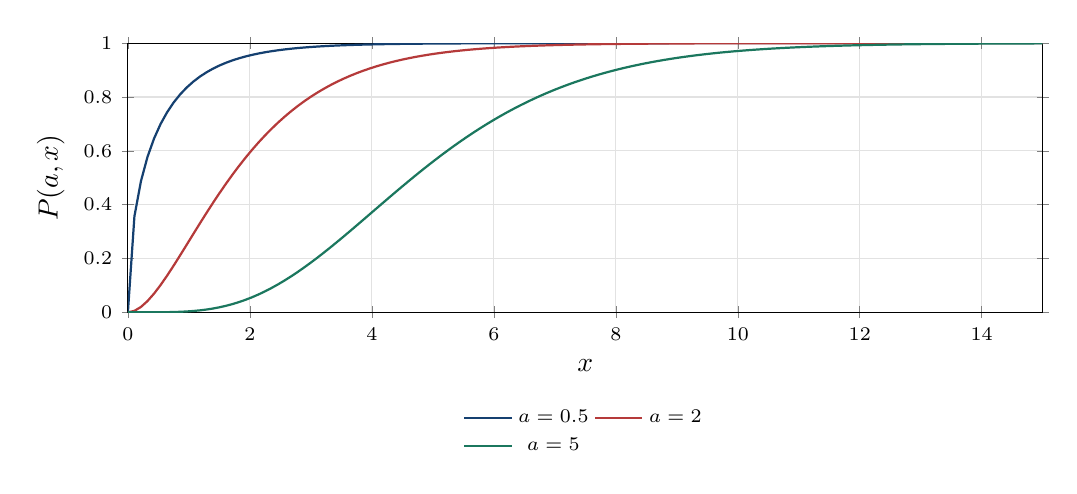
\begin{tikzpicture}\begin{axis}[base,axis lines=box,grid=major,minor tick num=0,width=13.2cm,height=5.0cm,xlabel={$x$},ylabel={$P(a,x)$},ymin=0,ymax=1,legend style={at={(0.5,-0.32)},anchor=north,legend columns=2,font=\scriptsize,draw=none,fill=white}]
\addplot[thick,azul,] coordinates {(0,0) (0.1071428571,0.3565711564) (0.2142857143,0.4873092397) (0.3214285714,0.5773219258) (0.4285714286,0.6454605202) (0.5357142857,0.6993770118) (0.6428571429,0.743160742) (0.75,0.7793286381) (0.8571428571,0.8095697362) (0.9642857143,0.8350851774) (1.071428571,0.8567650925) (1.178571429,0.8752895873) (1.285714286,0.89119057) (1.392857143,0.9048917205) (1.5,0.9167354833) (1.607142857,0.9270019546) (1.714285714,0.9359224935) (1.821428571,0.9436897777) (1.928571429,0.9504653866) (2.035714286,0.9563856262) (2.142857143,0.9615660698) (2.25,0.9661051465) (2.357142857,0.9700870097) (2.464285714,0.9735838532) (2.571428571,0.976657798) (2.678571429,0.9793624418) (2.785714286,0.9817441394) (2.892857143,0.9838430687) (3,0.9856941216) (3.107142857,0.9873276529) (3.214285714,0.9887701133) (3.321428571,0.9900445853) (3.428571429,0.991171239) (3.535714286,0.9921677218) (3.642857143,0.9930494911) (3.75,0.9938301007) (3.857142857,0.9945214468) (3.964285714,0.9951339799) (4.071428571,0.9956768888) (4.178571429,0.9961582585) (4.285714286,0.9965852088) (4.392857143,0.9969640134) (4.5,0.9973002039) (4.607142857,0.9975986612) (4.714285714,0.9978636936) (4.821428571,0.9980991067) (4.928571429,0.9983082637) (5.035714286,0.9984941377) (5.142857143,0.9986593589) (5.25,0.9988062546) (5.357142857,0.9989368851) (5.464285714,0.9990530752) (5.571428571,0.9991564414) (5.678571429,0.9992484164) (5.785714286,0.9993302706) (5.892857143,0.9994031301) (6,0.9994679945) (6.107142857,0.9995257504) (6.214285714,0.9995771848) (6.321428571,0.9996229966) (6.428571429,0.9996638065) (6.535714286,0.9997001656) (6.642857143,0.9997325639) (6.75,0.9997614365) (6.857142857,0.9997871706) (6.964285714,0.99981011) (7.071428571,0.9998305608) (7.178571429,0.999848795) (7.285714286,0.9998650548) (7.392857143,0.9998795555) (7.5,0.9998924888) (7.607142857,0.9999040254) (7.714285714,0.999914317) (7.821428571,0.999923499) (7.928571429,0.9999316918) (8.035714286,0.9999390026) (8.142857143,0.9999455269) (8.25,0.9999513499) (8.357142857,0.9999565474) (8.464285714,0.999961187) (8.571428571,0.9999653289) (8.678571429,0.9999690268) (8.785714286,0.9999723285) (8.892857143,0.9999752767) (9,0.9999779095) (9.107142857,0.9999802607) (9.214285714,0.9999823607) (9.321428571,0.9999842363) (9.428571429,0.9999859117) (9.535714286,0.9999874084) (9.642857143,0.9999887455) (9.75,0.99998994) (9.857142857,0.9999910073) (9.964285714,0.999991961) (10.07142857,0.9999928132) (10.17857143,0.9999935747) (10.28571429,0.9999942553) (10.39285714,0.9999948635) (10.5,0.9999954072) (10.60714286,0.9999958931) (10.71428571,0.9999963274) (10.82142857,0.9999967157) (10.92857143,0.9999970628) (11.03571429,0.9999973731) (11.14285714,0.9999976505) (11.25,0.9999978986) (11.35714286,0.9999981203) (11.46428571,0.9999983187) (11.57142857,0.999998496) (11.67857143,0.9999986546) (11.78571429,0.9999987964) (11.89285714,0.9999989232) (12,0.9999990366) (12.10714286,0.9999991381) (12.21428571,0.9999992288) (12.32142857,0.99999931) (12.42857143,0.9999993826) (12.53571429,0.9999994475) (12.64285714,0.9999995056) (12.75,0.9999995576) (12.85714286,0.9999996041) (12.96428571,0.9999996457) (13.07142857,0.9999996829) (13.17857143,0.9999997162) (13.28571429,0.999999746) (13.39285714,0.9999997727) (13.5,0.9999997965) (13.60714286,0.9999998179) (13.71428571,0.999999837) (13.82142857,0.9999998541) (13.92857143,0.9999998694) (14.03571429,0.9999998831) (14.14285714,0.9999998953) (14.25,0.9999999063) (14.35714286,0.9999999161) (14.46428571,0.9999999249) (14.57142857,0.9999999328) (14.67857143,0.9999999398) (14.78571429,0.9999999461) (14.89285714,0.9999999517) (15,0.9999999568)};
\addlegendentry{$a=0.5$}
\addplot[thick,rojo,] coordinates {(0,0) (0.1071428571,0.005345822793) (0.2142857143,0.01992845006) (0.3214285714,0.04181572817) (0.4285714286,0.06937277496) (0.5357142857,0.1012215184) (0.6428571429,0.1362053884) (0.75,0.1733585327) (0.8571428571,0.2118790009) (0.9642857143,0.2511054097) (1.071428571,0.2904966573) (1.178571429,0.3296143094) (1.285714286,0.368107322) (1.392857143,0.4056988096) (1.5,0.4421745996) (1.607142857,0.4773733469) (1.714285714,0.5111780099) (1.821428571,0.5435085137) (1.928571429,0.5743154464) (2.035714286,0.6035746545) (2.142857143,0.6312826208) (2.25,0.6574525202) (2.357142857,0.6821108637) (2.464285714,0.7052946531) (2.571428571,0.727048975) (2.678571429,0.7474249762) (2.785714286,0.7664781667) (2.892857143,0.7842670051) (3,0.8008517265) (3.107142857,0.8162933779) (3.214285714,0.8306530314) (3.321428571,0.843991149) (3.428571429,0.856367076) (3.535714286,0.8678386441) (3.642857143,0.8784618657) (3.75,0.8882907072) (3.857142857,0.8973769263) (3.964285714,0.9057699637) (4.071428571,0.9135168796) (4.178571429,0.9206623272) (4.285714286,0.9272485558) (4.392857143,0.9333154386) (4.5,0.938900519) (4.607142857,0.9440390729) (4.714285714,0.9487641814) (4.821428571,0.953106813) (4.928571429,0.9570959113) (5.035714286,0.9607584867) (5.142857143,0.9641197106) (5.25,0.96720301) (5.357142857,0.9700301624) (5.464285714,0.9726213891) (5.571428571,0.9749954463) (5.678571429,0.9771697147) (5.785714286,0.9791602847) (5.892857143,0.9809820396) (6,0.9826487348) (6.107142857,0.9841730729) (6.214285714,0.9855667763) (6.321428571,0.9868406547) (6.428571429,0.9880046698) (6.535714286,0.9890679962) (6.642857143,0.990039078) (6.75,0.9909256829) (6.857142857,0.9917349527) (6.964285714,0.9924734496) (7.071428571,0.9931472009) (7.178571429,0.9937617397) (7.285714286,0.9943221431) (7.392857143,0.9948330677) (7.5,0.9952987829) (7.607142857,0.9957232009) (7.714285714,0.9961099062) (7.821428571,0.9964621807) (7.928571429,0.9967830289) (8.035714286,0.9970752004) (8.142857143,0.9973412102) (8.25,0.9975833583) (8.357142857,0.9978037477) (8.464285714,0.9980043) (8.571428571,0.9981867711) (8.678571429,0.9983527649) (8.785714286,0.9985037461) (8.892857143,0.9986410516) (9,0.998765902) (9.107142857,0.9988794106) (9.214285714,0.9989825934) (9.321428571,0.9990763768) (9.428571429,0.9991616058) (9.535714286,0.9992390504) (9.642857143,0.9993094127) (9.75,0.9993733324) (9.857142857,0.9994313922) (9.964285714,0.9994841231) (10.07142857,0.9995320087) (10.17857143,0.999575489) (10.28571429,0.9996149651) (10.39285714,0.9996508017) (10.5,0.9996833308) (10.60714286,0.9997128547) (10.71428571,0.9997396482) (10.82142857,0.9997639613) (10.92857143,0.9997860215) (11.03571429,0.9998060356) (11.14285714,0.9998241916) (11.25,0.9998406606) (11.35714286,0.9998555979) (11.46428571,0.9998691447) (11.57142857,0.9998814294) (11.67857143,0.9998925686) (11.78571429,0.9999026683) (11.89285714,0.9999118247) (12,0.9999201252) (12.10714286,0.9999276493) (12.21428571,0.999934469) (12.32142857,0.9999406498) (12.42857143,0.9999462511) (12.53571429,0.9999513268) (12.64285714,0.999955926) (12.75,0.9999600931) (12.85714286,0.9999638684) (12.96428571,0.9999672885) (13.07142857,0.9999703866) (13.17857143,0.9999731928) (13.28571429,0.9999757345) (13.39285714,0.9999780364) (13.5,0.9999801211) (13.60714286,0.9999820089) (13.71428571,0.9999837183) (13.82142857,0.999985266) (13.92857143,0.9999866673) (14.03571429,0.999987936) (14.14285714,0.9999890845) (14.25,0.9999901242) (14.35714286,0.9999910652) (14.46428571,0.999991917) (14.57142857,0.999992688) (14.67857143,0.9999933857) (14.78571429,0.9999940171) (14.89285714,0.9999945885) (15,0.9999951056)};
\addlegendentry{$a=2$}
\addplot[thick,verde,] coordinates {(0,0) (0.1071428571,1.076238027e-07) (0.2142857143,3.150884433e-06) (0.3214285714,2.189603311e-05) (0.4285714286,8.445787234e-05) (0.5357142857,0.0002359812051) (0.6428571429,0.0005377481732) (0.75,0.001064677773) (0.8571428571,0.001901932721) (0.9642857143,0.003141151492) (1.071428571,0.004876669578) (1.178571429,0.007201975416) (1.285714286,0.01020655613) (1.392857143,0.01397322045) (1.5,0.01857593622) (1.607142857,0.02407818431) (1.714285714,0.0305318057) (1.821428571,0.03797630251) (1.928571429,0.04643854356) (2.035714286,0.05593282041) (2.142857143,0.06646119828) (2.25,0.07801410741) (2.357142857,0.09057112328) (2.464285714,0.1041018885) (2.571428571,0.1185671333) (2.678571429,0.1339197574) (2.785714286,0.1501059409) (2.892857143,0.1670662556) (3,0.1847367555) (3.107142857,0.2030500273) (3.214285714,0.2219361864) (3.321428571,0.2413238077) (3.428571429,0.2611407842) (3.535714286,0.2813151067) (3.642857143,0.3017755645) (3.75,0.3224523639) (3.857142857,0.3432776667) (3.964285714,0.364186051) (4.071428571,0.3851148975) (4.178571429,0.4060047038) (4.285714286,0.4267993339) (4.392857143,0.447446206) (4.5,0.4678964236) (4.607142857,0.488104857) (4.714285714,0.508030178) (4.821428571,0.5276348556) (4.928571429,0.5468851152) (5.035714286,0.5657508676) (5.142857143,0.5842056124) (5.25,0.6022263189) (5.357142857,0.6197932894) (5.464285714,0.6368900081) (5.571428571,0.6535029791) (5.678571429,0.6696215562) (5.785714286,0.6852377672) (5.892857143,0.7003461354) (6,0.7149434997) (6.107142857,0.7290288362) (6.214285714,0.7426030815) (6.321428571,0.7556689598) (6.428571429,0.7682308155) (6.535714286,0.7802944503) (6.642857143,0.7918669678) (6.75,0.8029566249) (6.857142857,0.8135726899) (6.964285714,0.8237253092) (7.071428571,0.8334253818) (7.178571429,0.842684441) (7.285714286,0.8515145453) (7.392857143,0.859928176) (7.5,0.8679381437) (7.607142857,0.8755575014) (7.714285714,0.8827994656) (7.821428571,0.8896773442) (7.928571429,0.8962044715) (8.035714286,0.9023941491) (8.142857143,0.9082595934) (8.25,0.9138138891) (8.357142857,0.9190699474) (8.464285714,0.9240404703) (8.571428571,0.9287379187) (8.678571429,0.9331744858) (8.785714286,0.9373620739) (8.892857143,0.9413122757) (9,0.9450363585) (9.107142857,0.9485452519) (9.214285714,0.9518495384) (9.321428571,0.9549594463) (9.428571429,0.9578848455) (9.535714286,0.9606352453) (9.642857143,0.9632197938) (9.75,0.9656472792) (9.857142857,0.9679261328) (9.964285714,0.9700644331) (10.07142857,0.9720699112) (10.17857143,0.9739499568) (10.28571429,0.9757116257) (10.39285714,0.9773616476) (10.5,0.9789064344) (10.60714286,0.9803520892) (10.71428571,0.9817044158) (10.82142857,0.9829689281) (10.92857143,0.9841508603) (11.03571429,0.9852551763) (11.14285714,0.9862865803) (11.25,0.9872495266) (11.35714286,0.9881482297) (11.46428571,0.9889866741) (11.57142857,0.9897686245) (11.67857143,0.9904976348) (11.78571429,0.9911770584) (11.89285714,0.9918100569) (12,0.9923996093) (12.10714286,0.9929485209) (12.21428571,0.9934594318) (12.32142857,0.993934825) (12.42857143,0.9943770348) (12.53571429,0.994788254) (12.64285714,0.9951705418) (12.75,0.9955258308) (12.85714286,0.9958559336) (12.96428571,0.9961625497) (13.07142857,0.9964472719) (13.17857143,0.9967115917) (13.28571429,0.9969569058) (13.39285714,0.997184521) (13.5,0.9973956597) (13.60714286,0.997591465) (13.71428571,0.9977730049) (13.82142857,0.9979412774) (13.92857143,0.9980972143) (14.03571429,0.9982416855) (14.14285714,0.9983755024) (14.25,0.9984994223) (14.35714286,0.9986141508) (14.46428571,0.998720346) (14.57142857,0.9988186207) (14.67857143,0.998909546) (14.78571429,0.9989936533) (14.89285714,0.9990714374) (15,0.9991433588)};
\addlegendentry{$a=5$}
\end{axis}\end{tikzpicture}
\caption{CDF gamma: todas son crecientes pese a que sus densidades tienen formas diferentes. Cambiar tasa reescala el argumento, no el parámetro de forma.}\label{fig:cdf-16}\end{figure}

\section{Casos enteros y relación con Poisson}
Para entero $m\ge1$, la recurrencia desde $Q(1,x)=e^{-x}$ da
\[
Q(m,x)=e^{-x}\sum_{k=0}^{m-1}\frac{x^k}{k!},\qquad
P(m,x)=1-Q(m,x).
\]
Si $N\sim\operatorname{Poisson}(x)$,
$Q(m,x)=\Pr(N\le m-1)$ y $P(m,x)=\Pr(N\ge m)$.

Para $m=3,x=2$,
\[
Q(3,2)=e^{-2}(1+2+2)=5e^{-2},\qquad P(3,2)=1-5e^{-2}.
\]
Para $x$ diminuto, calcular este complemento puede perder precisión: la serie positiva inferior calcula directamente una probabilidad de orden $x^m/m!$.

La función gamma incompleta es simultáneamente una CDF continua y una cola discreta. Las identidades permiten verificaciones cruzadas, pero conviene evitar usar dos rutas que comparten exactamente el mismo código como si fueran independientes.

\section{Semienteros y la normal}
Con $t=s^2$,
\[
P(1/2,x)=\erf(\sqrt x),\qquad Q(1/2,x)=\erfc(\sqrt x).
\]
Las recurrencias generan $a=3/2,5/2,\ldots$. Por ejemplo,
\[
Q(3/2,x)=\erfc(\sqrt x)+\frac{2\sqrt x}{\sqrt\pi}e^{-x},
\]
\[
Q(5/2,x)=\erfc(\sqrt x)+
\frac{2\sqrt x}{\sqrt\pi}e^{-x}\left(1+\frac{2x}3\right).
\]
La normal y la chi cuadrado de un grado están conectadas:
\[
\Pr(Z^2\le y)=2\Phi(\sqrt y)-1=P(1/2,y/2).
\]
Para valores pequeños, se evalúa una forma central de $\erf$ en lugar de restar dos cantidades próximas a uno.

\section{Asintótica de cola con parámetro fijo}
La integración por partes repetida da
\[
\Gamma(a,x)\sim e^{-x}x^{a-1}
\left[1+\frac{a-1}x+\frac{(a-1)(a-2)}{x^2}+\cdots\right]
\quad(x\to\infty).
\]
Después de $N$ términos, el resto exacto es
\[
(a-1)(a-2)\cdots(a-N)\Gamma(a-N,x).
\]
Para $x>0$, la gamma superior con parámetro desplazado sigue siendo una integral finita aunque el parámetro sea negativo, porque el origen queda excluido.

El signo y tamaño del resto dependen del parámetro. Para un entero positivo la expansión termina. Para un parámetro no entero puede ser asintótica divergente. Suponer que vale uniformemente cuando también $a$ crece es incorrecto: la transición $x\approx a$ requiere otra escala.

\section{La transición grande: del punto de silla a la normal}
Pongamos $x=a\lambda$ y definamos
\[
\eta=\sgn(\lambda-1)\sqrt{2(\lambda-1-\log\lambda)}.
\]
La cantidad interior es no negativa porque $\log\lambda\le\lambda-1$. El punto de silla está en $\lambda=1$. La variable $\eta$ transforma la fase
$\lambda-1-\log\lambda$ en una cuadrática $\eta^2/2$.

La expansión uniforme tiene término principal
\[
Q(a,a\lambda)\approx\frac12\erfc\left(\eta\sqrt{\frac a2}\right)
+\frac{e^{-a\eta^2/2}}{\sqrt{2\pi a}}
\left[\frac1{\lambda-1}-\frac1\eta\right].
\]
Los coeficientes posteriores son funciones suaves de $\eta$ y potencias de $1/a$. El primer término conecta gamma con normal; la corrección captura asimetría. La derivación completa separa la parte gaussiana de la amplitud transformada y expande esa amplitud alrededor del punto de silla.

Cerca de $\lambda=1$, las dos fracciones no se deben restar directamente. Con $\delta=\lambda-1$,
\[
\eta=\delta\left(1-\frac\delta3+\frac{7\delta^2}{36}+O(\delta^3)\right),
\quad
\frac1\delta-\frac1\eta=-\frac13+\frac\delta{12}+O(\delta^2).
\]
Por tanto $Q(a,a)\approx1/2-1/(3\sqrt{2\pi a})$. La expresión es una aproximación asintótica, no una garantía de precisión arbitraria con solo una corrección.

\section{Parámetro pequeño y una cola que desaparece}
Para $a\downarrow0$ y $x>0$ fijo, $\Gamma(a)\sim1/a$ y
\[
Q(a,x)\sim aE_1(x),\qquad
E_1(x)=\int_x^\infty\frac{e^{-t}}t\dd t.
\]
La CDF inferior se acerca a uno. Obtener $Q$ como $1-P$ puede perder el término de orden $a$, aunque $P$ tenga buen error absoluto.

La aproximación $\Gamma(a)\sim1/a$ se deduce de $\Gamma(a+1)=a\Gamma(a)$ y continuidad en uno. Para la integral superior, convergencia dominada con $x>0$ permite pasar al límite en $t^{a-1}$. La expansión no es uniforme cuando $x$ tiende simultáneamente a cero.

Para $x\downarrow0$ con $a>0$ fijo,
\[
P(a,x)\sim\frac{x^a}{\Gamma(a+1)}.
\]
Si $a$ es minúsculo, $x^a=\exp(a\log x)$ puede estar cerca de uno incluso para $x$ extremadamente pequeño. La intuición basada solo en el tamaño de $x$ falla.






\begin{figure}[htbp]\centering
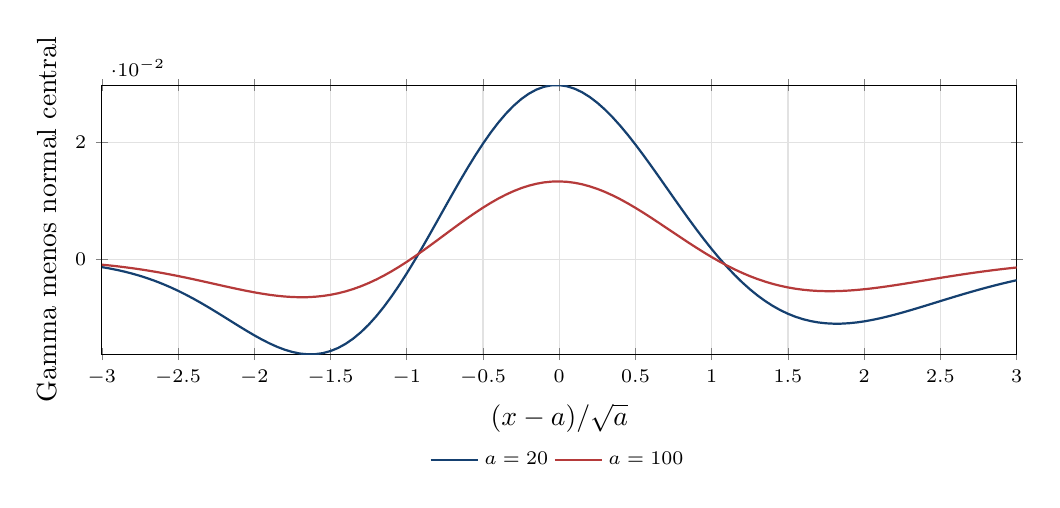
\begin{tikzpicture}\begin{axis}[base,axis lines=box,grid=major,minor tick num=0,width=13.2cm,height=5.0cm,xlabel={$(x-a)/\sqrt a$},ylabel={Gamma menos normal central},legend style={at={(0.5,-0.32)},anchor=north,legend columns=2,font=\scriptsize,draw=none,fill=white}]
\addplot[thick,azul,] coordinates {(-3,-0.00133068825) (-2.95,-0.001558464659) (-2.9,-0.001818707928) (-2.85,-0.002114431449) (-2.8,-0.002448536066) (-2.75,-0.002823701805) (-2.7,-0.003242264966) (-2.65,-0.003706082904) (-2.6,-0.004216389827) (-2.55,-0.00477364782) (-2.5,-0.005377398085) (-2.45,-0.006026118064) (-2.4,-0.006717090507) (-2.35,-0.007446290761) (-2.3,-0.008208298445) (-2.25,-0.008996239353) (-2.2,-0.009801762743) (-2.15,-0.0106150583) (-2.1,-0.01142491588) (-2.05,-0.01221882993) (-2,-0.01298314879) (-1.95,-0.01370326787) (-1.9,-0.01436386381) (-1.85,-0.01494916548) (-1.8,-0.01544325606) (-1.75,-0.01583039951) (-1.7,-0.01609538329) (-1.65,-0.01622386886) (-1.6,-0.01620274064) (-1.55,-0.01602044421) (-1.5,-0.01566730438) (-1.45,-0.01513581437) (-1.4,-0.01442088783) (-1.35,-0.01352006654) (-1.3,-0.0124336777) (-1.25,-0.0111649359) (-1.2,-0.009719986636) (-1.15,-0.008107889452) (-1.1,-0.006340540506) (-1.05,-0.004432535915) (-1,-0.002400978675) (-0.95,-0.0002652333408) (-0.9,0.001953366061) (-0.85,0.004231848396) (-0.8,0.006545970642) (-0.75,0.008870607923) (-0.7,0.01118015982) (-0.65,0.01344896428) (-0.6,0.01565171033) (-0.55,0.01776384123) (-0.5,0.01976193981) (-0.45,0.02162408875) (-0.4,0.02333019884) (-0.35,0.02486229966) (-0.3,0.02620478763) (-0.25,0.0273446279) (-0.2,0.02827150725) (-0.15,0.02897793659) (-0.1,0.02945930272) (-0.05,0.02971386993) (0,0.02974273316) (0.05,0.02954972546) (0.1,0.02914128301) (0.15,0.02852627208) (0.2,0.02771578253) (0.25,0.02672289306) (0.3,0.02556241387) (0.35,0.02425061223) (0.4,0.02280492688) (0.45,0.02124367685) (0.5,0.0195857701) (0.55,0.01785041736) (0.6,0.01605685572) (0.65,0.0142240865) (0.7,0.01237063096) (0.75,0.01051430725) (0.8,0.008672031167) (0.85,0.006859642517) (0.9,0.005091758721) (0.95,0.003381656199) (1,0.0017411798) (1.05,0.0001806798883) (1.1,-0.001291023784) (1.15,-0.002666652719) (1.2,-0.003940456516) (1.25,-0.005108177931) (1.3,-0.006166998391) (1.35,-0.007115466411) (1.4,-0.007953411483) (1.45,-0.008681846032) (1.5,-0.009302858086) (1.55,-0.009819497198) (1.6,-0.01023565611) (1.65,-0.01055595045) (1.7,-0.01078559868) (1.75,-0.01093030412) (1.8,-0.01099614092) (1.85,-0.01098944536) (1.9,-0.01091671374) (1.95,-0.01078450798) (2,-0.01059936947) (2.05,-0.01036774195) (2.1,-0.01009590357) (2.15,-0.009789908305) (2.2,-0.009455536725) (2.25,-0.009098255758) (2.3,-0.008723187238) (2.35,-0.008335084668) (2.4,-0.007938317673) (2.45,-0.007536863495) (2.5,-0.007134304844) (2.55,-0.006733833392) (2.6,-0.006338258178) (2.65,-0.005950018199) (2.7,-0.005571198471) (2.75,-0.005203548892) (2.8,-0.004848505244) (2.85,-0.00450721176) (2.9,-0.004180544688) (2.95,-0.003869136368) (3,-0.003573399397)};
\addlegendentry{$a=20$}
\addplot[thick,rojo,] coordinates {(-3,-0.0009195254367) (-2.95,-0.001049244372) (-2.9,-0.001192472699) (-2.85,-0.001349772185) (-2.8,-0.001521575596) (-2.75,-0.001708156738) (-2.7,-0.001909599244) (-2.65,-0.002125764711) (-2.6,-0.002356260908) (-2.55,-0.002600410877) (-2.5,-0.002857223828) (-2.45,-0.003125368834) (-2.4,-0.003403152339) (-2.35,-0.003688500546) (-2.3,-0.003978947757) (-2.25,-0.004271631662) (-2.2,-0.004563296538) (-2.15,-0.0048503052) (-2.1,-0.005128660376) (-2.05,-0.005394036029) (-2,-0.005641818913) (-1.95,-0.005867160406) (-1.9,-0.006065038396) (-1.85,-0.006230328716) (-1.8,-0.006357885313) (-1.75,-0.006442628044) (-1.7,-0.006479636723) (-1.65,-0.006464249727) (-1.6,-0.006392165288) (-1.55,-0.006259543334) (-1.5,-0.006063105617) (-1.45,-0.005800231763) (-1.4,-0.005469048811) (-1.35,-0.005068511851) (-1.3,-0.004598473446) (-1.25,-0.004059739678) (-1.2,-0.003454110888) (-1.15,-0.00278440546) (-1.1,-0.00205446533) (-1.05,-0.001269142313) (-1,-0.000434264745) (-0.95,0.0004434155882) (-0.9,0.001356295804) (-0.85,0.002296012646) (-0.8,0.003253550211) (-0.75,0.004219362869) (-0.7,0.00518351118) (-0.65,0.006135808237) (-0.6,0.007065973626) (-0.55,0.007963791906) (-0.5,0.008819272444) (-0.45,0.009622807315) (-0.4,0.01036532403) (-0.35,0.01103842998) (-0.3,0.01163454556) (-0.25,0.01214702335) (-0.2,0.01257025095) (-0.15,0.01289973539) (-0.1,0.01313216768) (-0.05,0.01326546616) (0,0.01329879828) (0.05,0.01323258041) (0.1,0.01306845616) (0.15,0.01280925395) (0.2,0.01245892508) (0.25,0.01202246394) (0.3,0.01150581229) (0.35,0.01091574994) (0.4,0.01025977429) (0.45,0.009545971363) (0.5,0.008782881117) (0.55,0.007979359793) (0.6,0.007144441981) (0.65,0.00628720508) (0.7,0.005416638571) (0.75,0.004541520366) (0.8,0.003670302214) (0.85,0.00281100588) (0.9,0.001971131471) (0.95,0.001157578996) (1,0.0003765838714) (1.05,-0.0003663332161) (1.1,-0.001066402006) (1.15,-0.001719624154) (1.2,-0.002322780998) (1.25,-0.002873428364) (1.3,-0.003369879362) (1.35,-0.003811176309) (1.4,-0.004197053073) (1.45,-0.004527889196) (1.5,-0.004804657256) (1.55,-0.005028864912) (1.6,-0.005202493114) (1.65,-0.00532793186) (1.7,-0.00540791488) (1.75,-0.005445454464) (1.8,-0.005443777601) (1.85,-0.005406264429) (1.9,-0.005336389866) (1.95,-0.00523766916) (2,-0.005113607942) (2.05,-0.004967657213) (2.1,-0.004803173564) (2.15,-0.004623384806) (2.2,-0.004431361044) (2.25,-0.004229991122) (2.3,-0.004021964298) (2.35,-0.003809756875) (2.4,-0.003595623489) (2.45,-0.003381592682) (2.5,-0.003169466343) (2.55,-0.002960822587) (2.6,-0.002757021616) (2.65,-0.002559214116) (2.7,-0.002368351731) (2.75,-0.002185199188) (2.8,-0.002010347671) (2.85,-0.001844229051) (2.9,-0.001687130628) (2.95,-0.001539210081) (3,-0.001400510336)};
\addlegendentry{$a=100$}
\end{axis}\end{tikzpicture}
\caption{Error de la aproximación normal central de gamma. La asimetría disminuye al crecer la forma. Una expansión de punto de silla incorpora una corrección que esta aproximación básica omite.}\label{fig:cdf-17}\end{figure}

\section{Derivadas y sensibilidad en parámetros}
Para $x>0$,
\[
\partial_xP(a,x)=\frac{x^{a-1}e^{-x}}{\Gamma(a)}.
\]
Definimos digamma $\psi(a)=\partial_a\log\Gamma(a)$. Diferenciando bajo la integral con parámetros en un compacto positivo,
\[
\partial_aP(a,x)=\frac1{\Gamma(a)}
\int_0^x t^{a-1}e^{-t}[\log t-\psi(a)]\dd t.
\]
La singularidad logarítmica en cero sigue siendo integrable para $a>0$. No se obtiene esta derivada simplemente multiplicando la densidad por una constante.

Para forma-tasa, $F(y;a,\lambda)=P(a,\lambda y)$ y
$\partial_\lambda F=y\,\partial_xP(a,\lambda y)$.
Para escala $\theta=1/\lambda$, $F=P(a,y/\theta)$ y el signo de la derivada cambia:
$\partial_\theta F=-(y/\theta^2)\partial_xP$.

Las derivadas de log-colas se evalúan con cocientes escalados para evitar dividir dos números subdesbordados.

\section{Diseño híbrido gamma y comprobaciones}
Un evaluador educativo usa serie inferior donde converge rápido, fracción superior donde es favorable, casos exactos enteros/semienteros y una expansión uniforme para forma grande cerca de la transición. Si se solicita la cola pequeña, se evita reconstruirla por resta cuando esa resta perdería dígitos.

Comprobaciones:
\[
P(a,0)=0,\quad Q(a,0)=1,\quad P+Q=1,\quad
\partial_xP>0,\quad
Q(a+1,x)-Q(a,x)=\frac{x^ae^{-x}}{\Gamma(a+1)}.
\]
Se comparan casos exactos, integración transformada y precisión ampliada. La documentación de R consultada describe su propia rutina gamma, por lo que no se afirma que sea idéntica a la versión didáctica serie/fracción expuesta aquí.


\parte{X. Beta incompleta, Fisher y distribuciones relacionadas}
\section{Beta desde dos gammas independientes}
Sean $U\sim\Gamma(a,1)$, $V\sim\Gamma(b,1)$ independientes. Pongamos $R=U+V$, $T=U/(U+V)$, de modo que $U=RT$, $V=R(1-T)$. El jacobiano absoluto es $R$. La densidad conjunta transformada es
\[
\frac{r^{a+b-1}e^{-r}}{\Gamma(a)\Gamma(b)}
t^{a-1}(1-t)^{b-1},\qquad r>0,\ 0<t<1.
\]
Usando la identidad beta-gamma, factoriza en una gamma de forma $a+b$ y una beta:
\[
f_T(t)=\frac{t^{a-1}(1-t)^{b-1}}{B(a,b)}.
\]
Además $R,T$ son independientes. La independencia proviene de la factorización; no se presume solo porque las variables originales lo eran.

La CDF es $I_x(a,b)$ para $0<x<1$, cero a la izquierda y uno a la derecha. Para $a<1$ o $b<1$ la densidad puede divergir en un extremo, sin que la masa deje de ser finita.

\section{Simetría y momentos beta}
El cambio $t=1-s$ da
\[
I_x(a,b)=1-I_{1-x}(b,a).
\]
Esta identidad permite escoger el lado con menor dificultad o calcular una cola pequeña directamente. En computadora conviene conservar $x$ y $1-x$ con la mayor exactitud disponible, sobre todo si el primero ya está redondeado a uno.

Los momentos se deducen de integrales beta:
\[
\E[T^k]=\frac{B(a+k,b)}{B(a,b)}
=\frac{(a)_k}{(a+b)_k}.
\]
Por tanto
\[
\E T=\frac a{a+b},\quad
\E T^2=\frac{a(a+1)}{(a+b)(a+b+1)},\quad
\Var T=\frac{ab}{(a+b)^2(a+b+1)}.
\]
La notación $(a)_k=a(a+1)\cdots(a+k-1)$ es el factorial ascendente, con $(a)_0=1$.

La media y la moda no coinciden. Si $a,b>1$, el máximo de la densidad está en $(a-1)/(a+b-2)$, derivando su logaritmo. En otros regímenes puede haber máximo en un extremo.






\begin{figure}[htbp]\centering
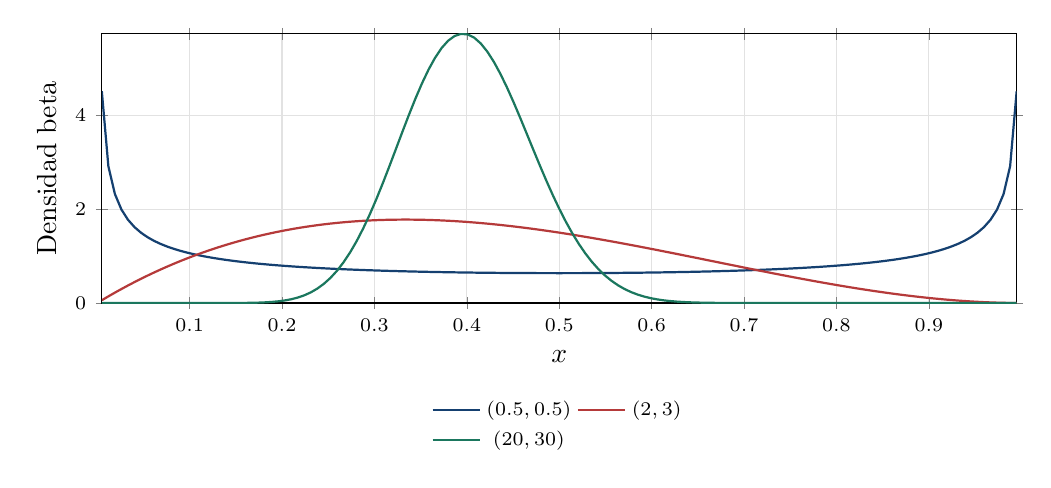
\begin{tikzpicture}\begin{axis}[base,axis lines=box,grid=major,minor tick num=0,width=13.2cm,height=5.0cm,xlabel={$x$},ylabel={Densidad beta},legend style={at={(0.5,-0.32)},anchor=north,legend columns=2,font=\scriptsize,draw=none,fill=white}]
\addplot[thick,azul,] coordinates {(0.005,4.512877914) (0.01207142857,2.914795028) (0.01914285714,2.322971431) (0.02621428571,1.992275588) (0.03328571429,1.774484126) (0.04035714286,1.617465789) (0.04742857143,1.497549995) (0.0545,1.40223599) (0.06157142857,1.324219264) (0.06864285714,1.258908966) (0.07571428571,1.203256156) (0.08278571429,1.155146381) (0.08985714286,1.113061195) (0.09692857143,1.075878355) (0.104,1.04274821) (0.1110714286,1.01301416) (0.1181428571,0.9861597527) (0.1252142857,0.9617724798) (0.1322857143,0.9395183789) (0.1393571429,0.9191238299) (0.1464285714,0.9003622542) (0.1535,0.8830442281) (0.1605714286,0.867010023) (0.1676428571,0.8521238972) (0.1747142857,0.838269674) (0.1817857143,0.8253472772) (0.1888571429,0.8132699876) (0.1959285714,0.8019622509) (0.203,0.7913579099) (0.2100714286,0.7813987672) (0.2171428571,0.7720334084) (0.2242142857,0.7632162319) (0.2312857143,0.7549066427) (0.2383571429,0.7470683799) (0.2454285714,0.7396689517) (0.2525,0.7326791579) (0.2595714286,0.7260726857) (0.2666428571,0.7198257642) (0.2737142857,0.7139168691) (0.2807857143,0.7083264685) (0.2878571429,0.7030368037) (0.2949285714,0.6980316996) (0.302,0.6932963991) (0.3090714286,0.6888174196) (0.3161428571,0.6845824268) (0.3232142857,0.6805801245) (0.3302857143,0.6768001573) (0.3373571429,0.6732330251) (0.3444285714,0.6698700075) (0.3515,0.6667030968) (0.3585714286,0.6637249387) (0.3656428571,0.6609287794) (0.3727142857,0.658308419) (0.3797857143,0.6558581691) (0.3868571429,0.6535728165) (0.3939285714,0.6514475893) (0.401,0.6494781273) (0.4080714286,0.6476604564) (0.4151428571,0.645990964) (0.4222142857,0.6444663789) (0.4292857143,0.6430837526) (0.4363571429,0.6418404427) (0.4434285714,0.6407340986) (0.4505,0.639762649) (0.4575714286,0.6389242906) (0.4646428571,0.6382174787) (0.4717142857,0.6376409196) (0.4787857143,0.6371935634) (0.4858571429,0.6368745992) (0.4929285714,0.6366834504) (0.5,0.6366197724) (0.5070714286,0.6366834504) (0.5141428571,0.6368745992) (0.5212142857,0.6371935634) (0.5282857143,0.6376409196) (0.5353571429,0.6382174787) (0.5424285714,0.6389242906) (0.5495,0.639762649) (0.5565714286,0.6407340986) (0.5636428571,0.6418404427) (0.5707142857,0.6430837526) (0.5777857143,0.6444663789) (0.5848571429,0.645990964) (0.5919285714,0.6476604564) (0.599,0.6494781273) (0.6060714286,0.6514475893) (0.6131428571,0.6535728165) (0.6202142857,0.6558581691) (0.6272857143,0.658308419) (0.6343571429,0.6609287794) (0.6414285714,0.6637249387) (0.6485,0.6667030968) (0.6555714286,0.6698700075) (0.6626428571,0.6732330251) (0.6697142857,0.6768001573) (0.6767857143,0.6805801245) (0.6838571429,0.6845824268) (0.6909285714,0.6888174196) (0.698,0.6932963991) (0.7050714286,0.6980316996) (0.7121428571,0.7030368037) (0.7192142857,0.7083264685) (0.7262857143,0.7139168691) (0.7333571429,0.7198257642) (0.7404285714,0.7260726857) (0.7475,0.7326791579) (0.7545714286,0.7396689517) (0.7616428571,0.7470683799) (0.7687142857,0.7549066427) (0.7757857143,0.7632162319) (0.7828571429,0.7720334084) (0.7899285714,0.7813987672) (0.797,0.7913579099) (0.8040714286,0.8019622509) (0.8111428571,0.8132699876) (0.8182142857,0.8253472772) (0.8252857143,0.838269674) (0.8323571429,0.8521238972) (0.8394285714,0.867010023) (0.8465,0.8830442281) (0.8535714286,0.9003622542) (0.8606428571,0.9191238299) (0.8677142857,0.9395183789) (0.8747857143,0.9617724798) (0.8818571429,0.9861597527) (0.8889285714,1.01301416) (0.896,1.04274821) (0.9030714286,1.075878355) (0.9101428571,1.113061195) (0.9172142857,1.155146381) (0.9242857143,1.203256156) (0.9313571429,1.258908966) (0.9384285714,1.324219264) (0.9455,1.40223599) (0.9525714286,1.497549995) (0.9596428571,1.617465789) (0.9667142857,1.774484126) (0.9737857143,1.992275588) (0.9808571429,2.322971431) (0.9879285714,2.914795028) (0.995,4.512877914)};
\addlegendentry{$(0.5,0.5)$}
\addplot[thick,rojo,] coordinates {(0.005,0.0594015) (0.01207142857,0.141380986) (0.01914285714,0.2210036888) (0.02621428571,0.2982950679) (0.03328571429,0.3732805832) (0.04035714286,0.4459856944) (0.04742857143,0.5164358613) (0.0545,0.5846565435) (0.06157142857,0.6506732009) (0.06864285714,0.7145112931) (0.07571428571,0.7761962799) (0.08278571429,0.835753621) (0.08985714286,0.8932087763) (0.09692857143,0.9485872054) (0.104,1.001914368) (0.1110714286,1.053215724) (0.1181428571,1.102516733) (0.1252142857,1.149842855) (0.1322857143,1.195219549) (0.1393571429,1.238672276) (0.1464285714,1.280226494) (0.1535,1.319907665) (0.1605714286,1.357741246) (0.1676428571,1.393752699) (0.1747142857,1.427967483) (0.1817857143,1.460411058) (0.1888571429,1.491108883) (0.1959285714,1.520086419) (0.203,1.547369124) (0.2100714286,1.572982459) (0.2171428571,1.596951883) (0.2242142857,1.619302857) (0.2312857143,1.640060839) (0.2383571429,1.65925129) (0.2454285714,1.67689967) (0.2525,1.693031437) (0.2595714286,1.707672053) (0.2666428571,1.720846976) (0.2737142857,1.732581666) (0.2807857143,1.742901584) (0.2878571429,1.751832188) (0.2949285714,1.759398939) (0.302,1.765627296) (0.3090714286,1.770542719) (0.3161428571,1.774170668) (0.3232142857,1.776536603) (0.3302857143,1.777665982) (0.3373571429,1.777584267) (0.3444285714,1.776316917) (0.3515,1.77388939) (0.3585714286,1.770327149) (0.3656428571,1.765655651) (0.3727142857,1.759900357) (0.3797857143,1.753086726) (0.3868571429,1.745240218) (0.3939285714,1.736386294) (0.401,1.726550412) (0.4080714286,1.715758032) (0.4151428571,1.704034615) (0.4222142857,1.69140562) (0.4292857143,1.677896506) (0.4363571429,1.663532733) (0.4434285714,1.648339762) (0.4505,1.632343052) (0.4575714286,1.615568062) (0.4646428571,1.598040252) (0.4717142857,1.579785082) (0.4787857143,1.560828013) (0.4858571429,1.541194503) (0.4929285714,1.520910012) (0.5,1.5) (0.5070714286,1.478489927) (0.5141428571,1.456405252) (0.5212142857,1.433771436) (0.5282857143,1.410613938) (0.5353571429,1.386958217) (0.5424285714,1.362829734) (0.5495,1.338253948) (0.5565714286,1.31325632) (0.5636428571,1.287862307) (0.5707142857,1.262097372) (0.5777857143,1.235986972) (0.5848571429,1.209556569) (0.5919285714,1.182831621) (0.599,1.155837588) (0.6060714286,1.128599931) (0.6131428571,1.101144108) (0.6202142857,1.07349558) (0.6272857143,1.045679807) (0.6343571429,1.017722247) (0.6414285714,0.9896483615) (0.6485,0.9614836095) (0.6555714286,0.9332534508) (0.6626428571,0.9049833452) (0.6697142857,0.8766987524) (0.6767857143,0.8484251321) (0.6838571429,0.8201879441) (0.6909285714,0.7920126482) (0.698,0.763924704) (0.7050714286,0.7359495713) (0.7121428571,0.7081127099) (0.7192142857,0.6804395795) (0.7262857143,0.6529556398) (0.7333571429,0.6256863506) (0.7404285714,0.5986571716) (0.7475,0.5718935625) (0.7545714286,0.5454209831) (0.7616428571,0.5192648932) (0.7687142857,0.4934507525) (0.7757857143,0.4680040206) (0.7828571429,0.4429501574) (0.7899285714,0.4183146226) (0.797,0.394122876) (0.8040714286,0.3704003772) (0.8111428571,0.3471725861) (0.8182142857,0.3244649623) (0.8252857143,0.3023029656) (0.8323571429,0.2807120557) (0.8394285714,0.2597176925) (0.8465,0.2393453355) (0.8535714286,0.2196204446) (0.8606428571,0.2005684795) (0.8677142857,0.1822149) (0.8747857143,0.1645851657) (0.8818571429,0.1477047365) (0.8889285714,0.131599072) (0.896,0.116293632) (0.9030714286,0.1018138763) (0.9101428571,0.08818526452) (0.9172142857,0.07543325651) (0.9242857143,0.06358331195) (0.9313571429,0.05266089061) (0.9384285714,0.04269145221) (0.9455,0.0337004565) (0.9525714286,0.02571336322) (0.9596428571,0.01875563211) (0.9667142857,0.0128527229) (0.9737857143,0.008030095351) (0.9808571429,0.00431320919) (0.9879285714,0.001727524159) (0.995,0.0002985)};
\addlegendentry{$(2,3)$}
\addplot[thick,verde,] coordinates {(0.005,9.327620124e-30) (0.01207142857,1.422089599e-22) (0.01914285714,7.364899901e-19) (0.02621428571,2.344944356e-16) (0.03328571429,1.774259436e-14) (0.04035714286,5.573636929e-13) (0.04742857143,9.666321597e-12) (0.0545,1.091916509e-10) (0.06157142857,8.918919277e-10) (0.06864285714,5.65137797e-09) (0.07571428571,2.918980326e-08) (0.08278571429,1.274317158e-07) (0.08985714286,4.832238007e-07) (0.09692857143,1.625536853e-06) (0.104,4.932159964e-06) (0.1110714286,1.367903042e-05) (0.1181428571,3.505598865e-05) (0.1252142857,8.376140189e-05) (0.1322857143,0.0001879936123) (0.1393571429,0.0003988347214) (0.1464285714,0.0008041153035) (0.1535,0.001547791845) (0.1605714286,0.002855599162) (0.1676428571,0.005067211874) (0.1747142857,0.008674348142) (0.1817857143,0.01436320547) (0.1888571429,0.02305841288) (0.1959285714,0.03596444604) (0.203,0.05459934938) (0.2100714286,0.08081482998) (0.2171428571,0.1167965119) (0.2242142857,0.1650385159) (0.2312857143,0.2282876417) (0.2383571429,0.3094542899) (0.2454285714,0.4114897728) (0.2525,0.5372326592) (0.2595714286,0.6892300136) (0.2666428571,0.8695425157) (0.2737142857,1.07954515) (0.2807857143,1.319737118) (0.2878571429,1.589575579) (0.2949285714,1.887347604) (0.302,2.210093254) (0.3090714286,2.553589997) (0.3161428571,2.912404998) (0.3232142857,3.280017358) (0.3302857143,3.649007521) (0.3373571429,4.011306262) (0.3444285714,4.358491229) (0.3515,4.682115434) (0.3585714286,4.974049504) (0.3656428571,5.226818353) (0.3727142857,5.433913052) (0.3797857143,5.590060263) (0.3868571429,5.691434365) (0.3939285714,5.735801139) (0.401,5.722586366) (0.4080714286,5.652867393) (0.4151428571,5.529290489) (0.4222142857,5.355921078) (0.4292857143,5.13803765) (0.4363571429,4.881882808) (0.4434285714,4.594386669) (0.4505,4.282878397) (0.4575714286,3.954801204) (0.4646428571,3.617444773) (0.4717142857,3.277706886) (0.4787857143,2.941893346) (0.4858571429,2.61556228) (0.4929285714,2.303415813) (0.5,2.009239164) (0.5070714286,1.735884624) (0.5141428571,1.485295682) (0.5212142857,1.258565015) (0.5282857143,1.056019006) (0.5353571429,0.8773210439) (0.5424285714,0.7215859574) (0.5495,0.5874984556) (0.5565714286,0.4734293595) (0.5636428571,0.3775445168) (0.5707142857,0.2979025421) (0.5777857143,0.2325387899) (0.5848571429,0.179534172) (0.5919285714,0.1370684968) (0.599,0.1034589004) (0.6060714286,0.07718462297) (0.6131428571,0.05689986015) (0.6202142857,0.04143669252) (0.6272857143,0.02980019493) (0.6343571429,0.02115777539) (0.6414285714,0.01482463154) (0.6485,0.01024697333) (0.6555714286,0.006984377477) (0.6626428571,0.004692342575) (0.6697142857,0.003105825318) (0.6767857143,0.002024276303) (0.6838571429,0.001298469139) (0.6909285714,0.0008192345177) (0.698,0.0005080726327) (0.7050714286,0.0003095203471) (0.7121428571,0.0001850887661) (0.7192142857,0.0001085561572) (0.7262857143,6.239365674e-05) (0.7333571429,3.511034528e-05) (0.7404285714,1.932419298e-05) (0.7475,1.039116547e-05) (0.7545714286,5.452638076e-06) (0.7616428571,2.788460405e-06) (0.7687142857,1.387781101e-06) (0.7757857143,6.711202292e-07) (0.7828571429,3.148184437e-07) (0.7899285714,1.429824479e-07) (0.797,6.274290645e-08) (0.8040714286,2.654023661e-08) (0.8111428571,1.079419056e-08) (0.8182142857,4.208993981e-09) (0.8252857143,1.568475515e-09) (0.8323571429,5.565734623e-10) (0.8394285714,1.873020312e-10) (0.8465,5.950133745e-11) (0.8535714286,1.77491633e-11) (0.8606428571,4.941463705e-12) (0.8677142857,1.274985025e-12) (0.8747857143,3.02388952e-13) (0.8818571429,6.529118418e-14) (0.8889285714,1.26884987e-14) (0.896,2.189225257e-15) (0.9030714286,3.298328574e-16) (0.9101428571,4.251857693e-17) (0.9172142857,4.572181169e-18) (0.9242857143,3.971431326e-19) (0.9313571429,2.67267024e-20) (0.9384285714,1.318536985e-21) (0.9455,4.421189431e-23) (0.9525714286,9.05078327e-25) (0.9596428571,9.64376115e-27) (0.9667142857,4.155416587e-29) (0.9737857143,4.68682607e-32) (0.9808571429,5.904414544e-36) (0.9879285714,1.055013928e-41) (0.995,9.577233735e-53)};
\addlegendentry{$(20,30)$}
\end{axis}\end{tikzpicture}
\caption{Beta con formas simétricas, asimétricas y concentradas. Los parámetros modifican comportamiento de extremos y anchura central.}\label{fig:cdf-18}\end{figure}

\section{Serie directa por el binomio generalizado}
Para $|t|<1$,
\[
(1-t)^{b-1}=\sum_{k=0}^\infty
\frac{(1-b)_k}{k!}t^k.
\]
Se obtiene de Taylor o de la ecuación diferencial del factor. Integrando,
\[
B_x(a,b)=x^a\sum_{k=0}^\infty
\frac{(1-b)_kx^k}{k!(a+k)}
=\frac{x^a}a\,{}_2F_1(a,1-b;a+1;x).
\]
La función hipergeométrica se define por
\[
{}_2F_1(A,B;C;x)=\sum_{k=0}^\infty
\frac{(A)_k(B)_k}{(C)_k\,k!}x^k,
\quad |x|<1,
\]
cuando los denominadores no se anulan. El cociente de términos permite estudiar convergencia.

Si $b$ es entero positivo, $(1-b)_k$ se hace cero y la serie termina. Para $b$ grande no entero puede presentar signos y cancelaciones. Cerca de $x=1$ la convergencia puede ser lenta; la simetría desplaza el problema a $1-x$.

\section{Una serie beta positiva por transformación}
La identidad hipergeométrica de Euler, que se puede comprobar mediante su ecuación diferencial y valor inicial, da
\[
B_x(a,b)=\frac{x^a(1-x)^b}a
{}_2F_1(a+b,1;a+1;x).
\]
Como $(1)_k=k!$,
\[
I_x(a,b)=\frac{x^a(1-x)^b}{aB(a,b)}
\sum_{k=0}^\infty\frac{(a+b)_k}{(a+1)_k}x^k.
\]
Todos los términos son positivos para $a,b>0$, $0\le x<1$. Definiendo $t_0=1$,
\[
t_{k+1}=t_k\,x\frac{a+b+k}{a+1+k}.
\]
Para $b>1$, los cocientes disminuyen a $x$; para $b<1$, aumentan a $x$. Si sumamos hasta $N$ y
\[
r=x\max\left(1,\frac{a+b+N+1}{a+N+2}\right)<1,
\]
el resto es a lo sumo $t_{N+1}/(1-r)$. Multiplicando por el prefactor obtenemos una cota absoluta y dividiendo por la suma parcial una cota relativa de truncamiento.

El prefactor se calcula como
$a\log x+b\logonep(-x)-\log a-\log B(a,b)$.
Una suma enorme y un prefactor minúsculo pueden compensarse; evaluar su producto sin escalado puede ser inestable.

\section{Relaciones contiguas y la fracción beta}
Las series hipergeométricas satisfacen relaciones entre parámetros vecinos. Un ejemplo, verificable comparando coeficientes, es
\[
{}_2F_1(A,B;C;x)-{}_2F_1(A,B-1;C-1;x)
=\frac{A(C-B)x}{C(C-1)}
{}_2F_1(A+1,B;C+1;x).
\]
Se deduce usando
$(B-1)_k/(B)_k=(B-1)/(B+k-1)$ y
$(C)_k/(C-1)_k=(C+k-1)/(C-1)$.
Intercambiar $A,B$ da otra relación. Iterar cocientes de funciones contiguas genera la fracción de Gauss; aplicada a la representación beta produce
\[
I_x(a,b)=\frac{x^a(1-x)^b}{aB(a,b)}
\cfrac1{1+\cfrac{d_1}{1+\cfrac{d_2}{1+\cdots}}},
\]
\[
d_{2m}=\frac{m(b-m)x}{(a+2m-1)(a+2m)},\quad m\ge1,
\]
\[
d_{2m+1}=-\frac{(a+m)(a+b+m)x}{(a+2m)(a+2m+1)},\quad m\ge0.
\]
La igualdad es la representación estándar beta incompleta citada en DLMF. Los dos tipos de coeficiente corresponden a los dos desplazamientos contiguos; no son una serie de Taylor cortada.

El primer coeficiente es $d_1=-(a+b)x/(a+1)$. Al expandir el recíproco, el primer término de la fracción es $1+(a+b)x/(a+1)+\cdots$, coincidiendo con la serie positiva.

\section{Implementar dos actualizaciones por iteración}
El algoritmo Lentz procesa alternadamente $d_{2m}$ y $d_{2m+1}$. Es importante incluir primero $d_1$: si el bucle empieza en $d_2$ sin inicialización equivalente, la fracción calculada es otra.

Una inicialización común toma
$D=1-(a+b)x/(a+1)$, invierte $D$ y usa $H=D^{-1}$, con $C=1$. Para cada $m\ge1$, procesa el coeficiente par y después el impar. Cada actualización modifica $D,C$ y multiplica $H$ por $CD$.

La región
\[
x<\frac{a+1}{a+b+2}
\]
suele favorecer la fracción directa. Al otro lado se evalúa $I_{1-x}(b,a)$ y se complementa cuando corresponde. El umbral mejora convergencia; no garantiza por sí mismo que la salida directa sea siempre la cola menor para todo parámetro.

Límites de iteraciones, comprobación de denominadores y una ruta independiente son parte de una implementación fiable. Un criterio $|\Delta-1|<\tau$ es una estimación práctica de estabilización del convergente.

\section{Casos exactos y la familia binomial}
Si $a,b$ son enteros positivos y $n=a+b-1$,
\[
I_x(a,b)=\sum_{j=a}^{n}\binom njx^j(1-x)^{n-j}.
\]
Para probarlo, derivamos la suma: los términos se cancelan telescópicamente y queda
$n!x^{a-1}(1-x)^{b-1}/[(a-1)!(b-1)!]$, la densidad beta. Ambos lados valen cero en $x=0$.

Así, $I_x(a,b)=\Pr(K\ge a)$ para $K\sim\operatorname{Binomial}(n,x)$. En particular,
\[
I_x(1,b)=1-(1-x)^b,\qquad I_x(a,1)=x^a.
\]
Para $x$ pequeño, la primera se evalúa con
$-\expmone(b\logonep(-x))$.

Para $a=b=1/2$, $t=\sin^2\theta$ da
\[
I_x(1/2,1/2)=\frac2\pi\arcsin\sqrt x.
\]
Es un caso elemental pese a pertenecer a una familia cuya forma general requiere funciones especiales.






\begin{figure}[htbp]\centering
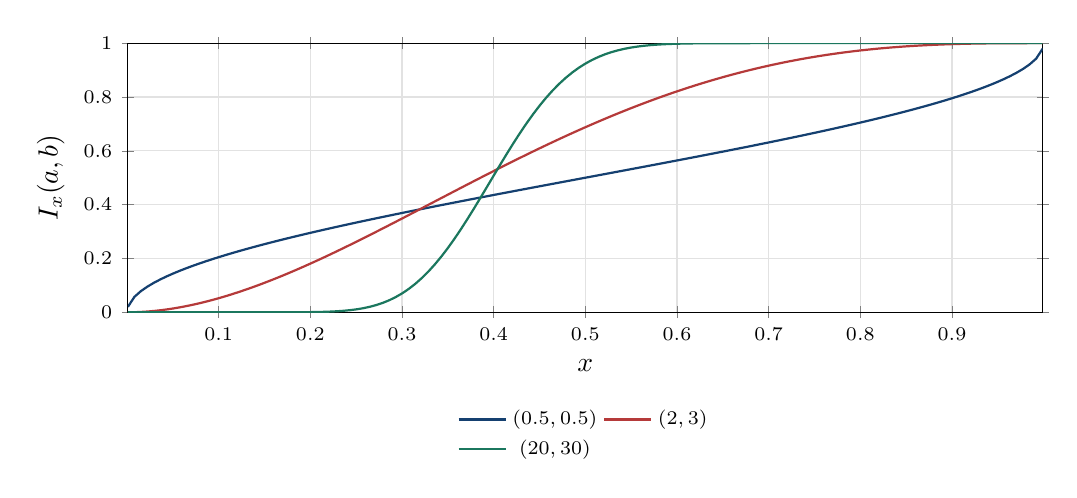
\begin{tikzpicture}\begin{axis}[base,axis lines=box,grid=major,minor tick num=0,width=13.2cm,height=5.0cm,xlabel={$x$},ylabel={$I_x(a,b)$},ymin=0,ymax=1,legend style={at={(0.5,-0.32)},anchor=north,legend columns=2,font=\scriptsize,draw=none,fill=white}]
\addplot[thick,azul,] coordinates {(0.001,0.02013504163) (0.008128571429,0.05747478605) (0.01525714286,0.07883649518) (0.02238571429,0.09560913733) (0.02951428571,0.109914776) (0.03664285714,0.1226206063) (0.04377142857,0.1341824995) (0.0509,0.1448751957) (0.05802857143,0.1548793979) (0.06515714286,0.1643214556) (0.07228571429,0.1732938122) (0.07941428571,0.1818665161) (0.08654285714,0.1900941493) (0.09367142857,0.1980202231) (0.1008,0.2056800884) (0.1079285714,0.2131029312) (0.1150571429,0.2203131822) (0.1221857143,0.2273315372) (0.1293142857,0.2341757131) (0.1364428571,0.2408610176) (0.1435714286,0.2474007868) (0.1507,0.2538067253) (0.1578285714,0.2600891751) (0.1649571429,0.2662573299) (0.1720857143,0.2723194082) (0.1792142857,0.2782827943) (0.1863428571,0.2841541545) (0.1934714286,0.2899395329) (0.2006,0.295644432) (0.2077285714,0.3012738804) (0.2148571429,0.3068324895) (0.2219857143,0.3123245029) (0.2291142857,0.3177538374) (0.2362428571,0.3231241196) (0.2433714286,0.3284387167) (0.2505,0.3337007636) (0.2576285714,0.3389131862) (0.2647571429,0.3440787227) (0.2718857143,0.3491999413) (0.2790142857,0.3542792565) (0.2861428571,0.3593189434) (0.2932714286,0.3643211504) (0.3004,0.3692879103) (0.3075285714,0.3742211511) (0.3146571429,0.3791227041) (0.3217857143,0.3839943131) (0.3289142857,0.3888376413) (0.3360428571,0.3936542782) (0.3431714286,0.3984457458) (0.3503,0.4032135039) (0.3574285714,0.4079589554) (0.3645571429,0.4126834511) (0.3716857143,0.4173882938) (0.3788142857,0.4220747424) (0.3859428571,0.4267440153) (0.3930714286,0.4313972943) (0.4002,0.4360357272) (0.4073285714,0.4406604313) (0.4144571429,0.4452724957) (0.4215857143,0.4498729843) (0.4287142857,0.4544629379) (0.4358428571,0.4590433768) (0.4429714286,0.4636153028) (0.4501,0.4681797016) (0.4572285714,0.4727375445) (0.4643571429,0.4772897904) (0.4714857143,0.4818373879) (0.4786142857,0.4863812769) (0.4857428571,0.4909223906) (0.4928714286,0.4954616567) (0.5,0.5) (0.5071285714,0.5045383433) (0.5142571429,0.5090776094) (0.5213857143,0.5136187231) (0.5285142857,0.5181626121) (0.5356428571,0.5227102096) (0.5427714286,0.5272624555) (0.5499,0.5318202984) (0.5570285714,0.5363846972) (0.5641571429,0.5409566232) (0.5712857143,0.5455370621) (0.5784142857,0.5501270157) (0.5855428571,0.5547275043) (0.5926714286,0.5593395687) (0.5998,0.5639642728) (0.6069285714,0.5686027057) (0.6140571429,0.5732559847) (0.6211857143,0.5779252576) (0.6283142857,0.5826117062) (0.6354428571,0.5873165489) (0.6425714286,0.5920410446) (0.6497,0.5967864961) (0.6568285714,0.6015542542) (0.6639571429,0.6063457218) (0.6710857143,0.6111623587) (0.6782142857,0.6160056869) (0.6853428571,0.6208772959) (0.6924714286,0.6257788489) (0.6996,0.6307120897) (0.7067285714,0.6356788496) (0.7138571429,0.6406810566) (0.7209857143,0.6457207435) (0.7281142857,0.6508000587) (0.7352428571,0.6559212773) (0.7423714286,0.6610868138) (0.7495,0.6662992364) (0.7566285714,0.6715612833) (0.7637571429,0.6768758804) (0.7708857143,0.6822461626) (0.7780142857,0.6876754971) (0.7851428571,0.6931675105) (0.7922714286,0.6987261196) (0.7994,0.704355568) (0.8065285714,0.7100604671) (0.8136571429,0.7158458455) (0.8207857143,0.7217172057) (0.8279142857,0.7276805918) (0.8350428571,0.7337426701) (0.8421714286,0.7399108249) (0.8493,0.7461932747) (0.8564285714,0.7525992132) (0.8635571429,0.7591389824) (0.8706857143,0.7658242869) (0.8778142857,0.7726684628) (0.8849428571,0.7796868178) (0.8920714286,0.7868970688) (0.8992,0.7943199116) (0.9063285714,0.8019797769) (0.9134571429,0.8099058507) (0.9205857143,0.8181334839) (0.9277142857,0.8267061878) (0.9348428571,0.8356785444) (0.9419714286,0.8451206021) (0.9491,0.8551248043) (0.9562285714,0.8658175005) (0.9633571429,0.8773793937) (0.9704857143,0.890085224) (0.9776142857,0.9043908627) (0.9847428571,0.9211635048) (0.9918714286,0.9425252139) (0.999,0.9798649584)};
\addlegendentry{$(0.5,0.5)$}
\addplot[thick,rojo,] coordinates {(0.001,5.992003e-06) (0.008128571429,0.0003921584614) (0.01525714286,0.001368432498) (0.02238571429,0.002917731119) (0.02951428571,0.005023157261) (0.03664285714,0.007667999784) (0.04377142857,0.01083573348) (0.0509,0.01451001906) (0.05802857143,0.01867470317) (0.06515714286,0.02331381837) (0.07228571429,0.02841158318) (0.07941428571,0.033952402) (0.08654285714,0.03992086519) (0.09367142857,0.04630174903) (0.1008,0.05308001572) (0.1079285714,0.0602408134) (0.1150571429,0.06776947612) (0.1221857143,0.07565152387) (0.1293142857,0.08387266256) (0.1364428571,0.09241878403) (0.1435714286,0.1012759661) (0.1507,0.1104304723) (0.1578285714,0.1198687525) (0.1649571429,0.129577442) (0.1720857143,0.1395433624) (0.1792142857,0.1497535212) (0.1863428571,0.1601951115) (0.1934714286,0.1708555127) (0.2006,0.18172229) (0.2077285714,0.1927831944) (0.2148571429,0.2040261631) (0.2219857143,0.2154393189) (0.2291142857,0.2270109708) (0.2362428571,0.2387296136) (0.2433714286,0.2505839279) (0.2505,0.2625627806) (0.2576285714,0.2746552242) (0.2647571429,0.2868504972) (0.2718857143,0.2991380241) (0.2790142857,0.3115074152) (0.2861428571,0.3239484669) (0.2932714286,0.3364511615) (0.3004,0.3490056669) (0.3075285714,0.3616023374) (0.3146571429,0.374231713) (0.3217857143,0.3868845196) (0.3289142857,0.3995516691) (0.3360428571,0.4122242592) (0.3431714286,0.4248935738) (0.3503,0.4375510823) (0.3574285714,0.4501884406) (0.3645571429,0.4627974899) (0.3716857143,0.4753702578) (0.3788142857,0.4878989577) (0.3859428571,0.5003759887) (0.3930714286,0.5127939362) (0.4002,0.5251455712) (0.4073285714,0.5374238508) (0.4144571429,0.5496219181) (0.4215857143,0.5617331019) (0.4287142857,0.5737509171) (0.4358428571,0.5856690645) (0.4429714286,0.5974814307) (0.4501,0.6091820884) (0.4572285714,0.6207652962) (0.4643571429,0.6322254986) (0.4714857143,0.6435573258) (0.4786142857,0.6547555944) (0.4857428571,0.6658153065) (0.4928714286,0.6767316503) (0.5,0.6875) (0.5071285714,0.6981159156) (0.5142571429,0.7085751431) (0.5213857143,0.7188736143) (0.5285142857,0.7290074472) (0.5356428571,0.7389729453) (0.5427714286,0.7487665986) (0.5499,0.7583850825) (0.5570285714,0.7678252585) (0.5641571429,0.7770841742) (0.5712857143,0.7861590629) (0.5784142857,0.7950473439) (0.5855428571,0.8037466226) (0.5926714286,0.81225469) (0.5998,0.8205695232) (0.6069285714,0.8286892853) (0.6140571429,0.8366123253) (0.6211857143,0.8443371779) (0.6283142857,0.851862564) (0.6354428571,0.8591873904) (0.6425714286,0.8663107497) (0.6497,0.8732319205) (0.6568285714,0.8799503672) (0.6639571429,0.8864657404) (0.6710857143,0.8927778764) (0.6782142857,0.8988867975) (0.6853428571,0.9047927119) (0.6924714286,0.9104960138) (0.6996,0.9159972832) (0.7067285714,0.9212972861) (0.7138571429,0.9263969745) (0.7209857143,0.9312974863) (0.7281142857,0.9360001452) (0.7352428571,0.9405064608) (0.7423714286,0.944818129) (0.7495,0.9489370311) (0.7566285714,0.9528652348) (0.7637571429,0.9566049934) (0.7708857143,0.9601587463) (0.7780142857,0.9635291187) (0.7851428571,0.9667189218) (0.7922714286,0.9697311529) (0.7994,0.9725689949) (0.8065285714,0.9752358167) (0.8136571429,0.9777351734) (0.8207857143,0.9800708057) (0.8279142857,0.9822466405) (0.8350428571,0.9842667903) (0.8421714286,0.9861355539) (0.8493,0.9878574157) (0.8564285714,0.9894370462) (0.8635571429,0.9908793019) (0.8706857143,0.992189225) (0.8778142857,0.9933720438) (0.8849428571,0.9944331725) (0.8920714286,0.9953782111) (0.8992,0.9962129458) (0.9063285714,0.9969433484) (0.9134571429,0.9975755769) (0.9205857143,0.998115975) (0.9277142857,0.9985710726) (0.9348428571,0.9989475852) (0.9419714286,0.9992524145) (0.9491,0.999492648) (0.9562285714,0.9996755591) (0.9633571429,0.9998086072) (0.9704857143,0.9998994377) (0.9776142857,0.9999558816) (0.9847428571,0.9999859563) (0.9918714286,0.9999978648) (0.999,0.999999996)};
\addlegendentry{$(2,3)$}
\addplot[thick,verde,] coordinates {(0.001,2.750687666e-47) (0.008128571429,3.579897118e-29) (0.01525714286,8.642607239e-24) (0.02238571429,1.512300306e-20) (0.02951428571,3.114159139e-18) (0.03664285714,1.924820347e-16) (0.04377142857,5.492276696e-15) (0.0509,9.142143473e-14) (0.05802857143,1.022582511e-12) (0.06515714286,8.427092923e-12) (0.07228571429,5.450859183e-11) (0.07941428571,2.895758184e-10) (0.08654285714,1.306707119e-09) (0.09367142857,5.138596308e-09) (0.1008,1.796545175e-08) (0.1079285714,5.673537793e-08) (0.1150571429,1.639310087e-07) (0.1221857143,4.379478882e-07) (0.1293142857,1.091246738e-06) (0.1364428571,2.554683408e-06) (0.1435714286,5.653965658e-06) (0.1507,1.189235367e-05) (0.1578285714,2.388132756e-05) (0.1649571429,4.596633181e-05) (0.1720857143,8.509588308e-05) (0.1792142857,0.0001519772273) (0.1863428571,0.0002625485602) (0.1934714286,0.000439775453) (0.2006,0.0007157474579) (0.2077285714,0.001134011131) (0.2148571429,0.001752030569) (0.2219857143,0.002643620053) (0.2291142857,0.0039011506) (0.2362428571,0.005637298862) (0.2433714286,0.007986088471) (0.2505,0.01110297537) (0.2576285714,0.01516375333) (0.2647571429,0.02036210485) (0.2718857143,0.02690569477) (0.2790142857,0.03501079583) (0.2861428571,0.04489553986) (0.2932714286,0.05677199901) (0.3004,0.07083740723) (0.3075285714,0.08726492499) (0.3146571429,0.1061944207) (0.3217857143,0.1277237823) (0.3289142857,0.1519012792) (0.3360428571,0.1787194616) (0.3431714286,0.20811102) (0.3503,0.2399469242) (0.3574285714,0.274037043) (0.3645571429,0.3101332978) (0.3716857143,0.3479352639) (0.3788142857,0.3870979878) (0.3859428571,0.4272416628) (0.3930714286,0.4679627038) (0.4002,0.5088456882) (0.4073285714,0.5494755936) (0.4144571429,0.5894497622) (0.4215857143,0.6283890534) (0.4287142857,0.6659477137) (0.4358428571,0.7018215805) (0.4429714286,0.7357543458) (0.4501,0.7675417206) (0.4572285714,0.7970334615) (0.4643571429,0.8241333314) (0.4714857143,0.8487971638) (0.4786142857,0.8710292826) (0.4857428571,0.8908775852) (0.4928714286,0.9084276344) (0.5,0.923796114) (0.5071285714,0.937123996) (0.5142571429,0.9485697388) (0.5213857143,0.958302794) (0.5285142857,0.9664976482) (0.5356428571,0.9733285687) (0.5427714286,0.9789651634) (0.5499,0.9835688093) (0.5570285714,0.9872899551) (0.5641571429,0.990266259) (0.5712857143,0.99262149) (0.5784142857,0.994465099) (0.5855428571,0.9958923479) (0.5926714286,0.9969848838) (0.5998,0.9978116426) (0.6069285714,0.9984299765) (0.6140571429,0.9988869114) (0.6211857143,0.9992204527) (0.6283142857,0.9994608761) (0.6354428571,0.9996319536) (0.6425714286,0.999752082) (0.6497,0.999835291) (0.6568285714,0.9998921228) (0.6639571429,0.9999303805) (0.6710857143,0.9999557521) (0.6782142857,0.9999723197) (0.6853428571,0.9999829666) (0.6924714286,0.999989696) (0.6996,0.9999938768) (0.7067285714,0.9999964281) (0.7138571429,0.9999979563) (0.7209857143,0.9999988541) (0.7281142857,0.9999993709) (0.7352428571,0.9999996622) (0.7423714286,0.9999998228) (0.7495,0.9999999093) (0.7566285714,0.9999999548) (0.7637571429,0.999999978) (0.7708857143,0.9999999896) (0.7780142857,0.9999999953) (0.7851428571,0.9999999979) (0.7922714286,0.9999999991) (0.7994,0.9999999996) (0.8065285714,0.9999999999) (0.8136571429,0.9999999999) (0.8207857143,1) (0.8279142857,1) (0.8350428571,1) (0.8421714286,1) (0.8493,1) (0.8564285714,1) (0.8635571429,1) (0.8706857143,1) (0.8778142857,1) (0.8849428571,1) (0.8920714286,1) (0.8992,1) (0.9063285714,1) (0.9134571429,1) (0.9205857143,1) (0.9277142857,1) (0.9348428571,1) (0.9419714286,1) (0.9491,1) (0.9562285714,1) (0.9633571429,1) (0.9704857143,1) (0.9776142857,1) (0.9847428571,1) (0.9918714286,1) (0.999,1)};
\addlegendentry{$(20,30)$}
\end{axis}\end{tikzpicture}
\caption{La CDF beta mantiene rango y monotonía en todos estos regímenes. Las singularidades del integrando no producen saltos de una distribución continua.}\label{fig:cdf-19}\end{figure}

\section{Recurrencias beta y dirección de estabilidad}
Integrando la derivada de $t^a(1-t)^b$ y combinando constantes de normalización,
\[
I_x(a,b)=I_x(a+1,b)+\frac{x^a(1-x)^b}{aB(a,b)},
\]
\[
I_x(a,b)=I_x(a,b+1)-\frac{x^a(1-x)^b}{bB(a,b)}.
\]
La primera implica que incrementar $a$ reduce la CDF para $x$ fijo; incrementar $b$ la aumenta. Estas afirmaciones también reflejan desplazamientos de la distribución.

Una recurrencia ascendente que resta cantidades casi iguales puede perder precisión. La dirección se selecciona según cuál cola se quiere y qué términos son pequeños. El término de borde se evalúa en logaritmos.

Las relaciones son exactas, pero un conjunto de identidades exactas no determina por sí solo una ruta numérica estable. Esta es la diferencia entre álgebra funcional y análisis de algoritmos.

\section{Parámetros grandes: concentración y fase}
Escribamos $a=n\mu$, $b=n(1-\mu)$ con $\mu$ separado de cero y uno. La densidad se concentra cerca de $\mu$ con desviación aproximadamente $\sqrt{\mu(1-\mu)/n}$. Para
\[
z=\frac{x-\mu}{\sqrt{\mu(1-\mu)/n}},
\]
una aproximación central es $I_x(a,b)\approx\Phi(z)$ cuando $z$ permanece acotado y $n\to\infty$. No es una aproximación relativa de colas arbitrariamente remotas.

Una variable de punto de silla usa
\[
D(\mu\Vert x)=\mu\log\frac\mu x+
(1-\mu)\log\frac{1-\mu}{1-x},
\quad \eta=\sgn(x-\mu)\sqrt{2D(\mu\Vert x)}.
\]
La fase queda $n\eta^2/2$ y una expansión uniforme conecta la integral beta con una función error más correcciones de amplitud.

El coeficiente de asimetría exacto es
\[
\gamma_1=\frac{2(b-a)\sqrt{a+b+1}}
{(a+b+2)\sqrt{ab}}.
\]
Una corrección central tipo Edgeworth contiene
$\gamma_1(1-z^2)\ph(z)/6$. Es una expansión bajo un régimen de parámetros grande y proporcional; cerca de extremos o en colas extremas se requiere otra aproximación.

\section{Derivar Fisher a partir de un cociente}
Sean $A=U/2\sim\Gamma(a,1)$, $B=V/2\sim\Gamma(b,1)$ independientes, con $a=d_1/2$, $b=d_2/2$. Para $R=A/B$, usemos $A=RB$; el jacobiano es $B$. Integrar $B$ da
\[
f_R(r)=\frac{r^{a-1}}{B(a,b)(1+r)^{a+b}},\quad r>0.
\]
Como $W=(b/a)R$, su densidad es
\[
f_W(w)=\frac{(a/b)^a}{B(a,b)}
w^{a-1}\left(1+\frac abw\right)^{-(a+b)}.
\]
El cambio $z=r/(1+r)=aw/(b+aw)$ convierte la integral en beta:
\[
F_{d_1,d_2}(w)=I_z(a,b).
\]
La supervivencia se calcula directamente como
$I_{b/(b+aw)}(b,a)$. No hace falta restar la CDF F de uno.

\section{Transformar Fisher sin desbordar}
Si $w$ es enorme, formar $aw$ puede desbordar. Definamos
$\ell=\log a+\log w-\log b$. Entonces $r=e^\ell$ y
\[
z=\frac r{1+r},\qquad y=\frac1{1+r}.
\]
Para $\ell\ge0$,
$z=1/(1+e^{-\ell})$, $y=e^{-\ell}/(1+e^{-\ell})$.
Para $\ell<0$,
$z=e^\ell/(1+e^\ell)$, $y=1/(1+e^\ell)$.
Conservamos ambos, sin reconstruir el pequeño por resta.

Aunque $z$ redondee a uno, $y$ puede seguir positivo. Un evaluador beta que recibe solo $z=1$ ya perdió información; una interfaz de cola o de argumentos complementarios puede preservarla.

La identidad de reciprocidad es
\[
F_{d_1,d_2}(w)=1-F_{d_2,d_1}(1/w),
\]
con el intercambio de grados. Es otra comprobación de las transformaciones.

\section{Fisher en casos simples y comportamiento de cola}
Para $d_1=d_2=2$, $a=b=1$, y
\[
F_{2,2}(w)=\frac w{1+w},\qquad S_{2,2}(w)=\frac1{1+w}.
\]
Para $d_1=d_2=1$,
\[
F_{1,1}(w)=\frac2\pi\arctan\sqrt w.
\]
La identidad surge de la beta $1/2,1/2$ y
$\arcsin\sqrt{w/(1+w)}=\arctan\sqrt w$.

En general, la densidad F se comporta como $Cw^{-b-1}$ en infinito y la supervivencia como $(C/b)w^{-b}$. La cola es polinómica, mucho más pesada que la normal. Cortar el dominio con una regla diseñada para exponenciales puede resultar costoso.

Los momentos $\E W^k$ existen solo si $b>k$:
\[
\E W^k=\left(\frac ba\right)^k
\frac{\Gamma(a+k)\Gamma(b-k)}{\Gamma(a)\Gamma(b)}.
\]
En particular $\E W=d_2/(d_2-2)$ para $d_2>2$. Una CDF existe aunque algunos momentos diverjan.






\begin{figure}[htbp]\centering
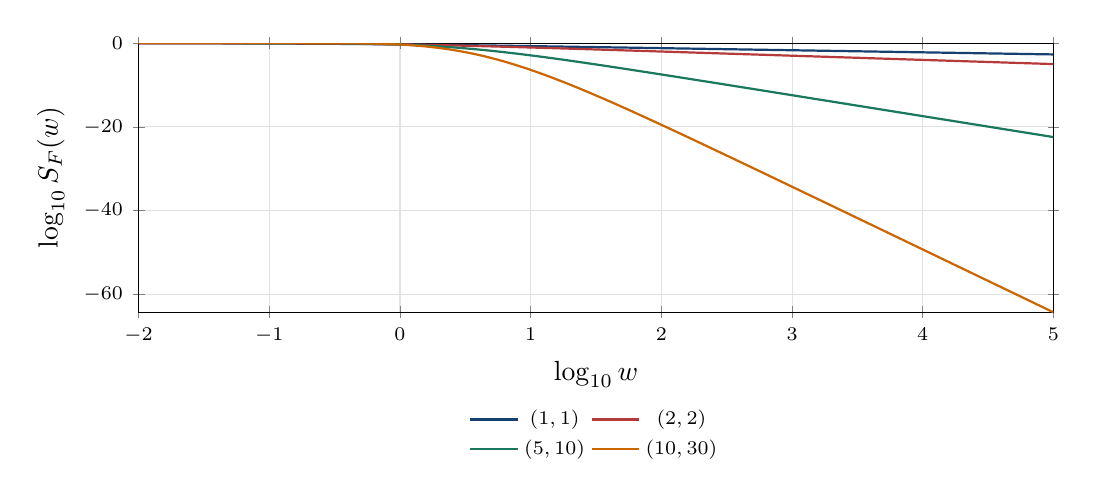
\begin{tikzpicture}\begin{axis}[base,axis lines=box,grid=major,minor tick num=0,width=13.2cm,height=5.0cm,xlabel={$\log_{10}w$},ylabel={$\log_{10}S_F(w)$},legend style={at={(0.5,-0.32)},anchor=north,legend columns=2,font=\scriptsize,draw=none,fill=white}]
\addplot[thick,azul,] coordinates {(-2,-0.02846951169) (-1.95,-0.03020385642) (-1.9,-0.03204618908) (-1.85,-0.03400343399) (-1.8,-0.03608296774) (-1.75,-0.03829264686) (-1.7,-0.04064083617) (-1.65,-0.04313643798) (-1.6,-0.04578892159) (-1.55,-0.04860835296) (-1.5,-0.05160542393) (-1.45,-0.0547914806) (-1.4,-0.05817855003) (-1.35,-0.06177936459) (-1.3,-0.06560738273) (-1.25,-0.06967680524) (-1.2,-0.0740025853) (-1.15,-0.07860043098) (-1.1,-0.08348679808) (-1.05,-0.08867887146) (-1,-0.09419453237) (-0.95,-0.1000523096) (-0.9,-0.1062713115) (-0.85,-0.1128711371) (-0.8,-0.119871763) (-0.75,-0.1272934045) (-0.7,-0.1351563493) (-0.65,-0.1434807629) (-0.6,-0.1522864655) (-0.55,-0.161592682) (-0.5,-0.1714177683) (-0.45,-0.181778918) (-0.4,-0.1926918563) (-0.35,-0.2041705289) (-0.3,-0.2162267967) (-0.25,-0.2288701466) (-0.2,-0.2421074313) (-0.15,-0.2559426494) (-0.1,-0.2703767775) (-0.05,-0.2854076648) (0,-0.3010299957) (0.05,-0.3172353257) (0.1,-0.3340121914) (0.15,-0.3513462893) (0.2,-0.3692207186) (0.25,-0.3876162765) (0.3,-0.4065117946) (0.35,-0.4258845016) (0.4,-0.4457103992) (0.45,-0.4659646366) (0.5,-0.4866218731) (0.55,-0.5076566159) (0.6,-0.5290435275) (0.65,-0.5507576965) (0.7,-0.5727748677) (0.75,-0.5950716318) (0.8,-0.6176255745) (0.85,-0.6404153882) (0.9,-0.663420948) (0.95,-0.6866233579) (1,-0.7100049691) (1.05,-0.7335493766) (1.1,-0.7572413976) (1.15,-0.7810670347) (1.2,-0.805013429) (1.25,-0.8290688042) (1.3,-0.8532224065) (1.35,-0.8774644409) (1.4,-0.9017860058) (1.45,-0.9261790283) (1.5,-0.9506362008) (1.55,-0.9751509189) (1.6,-0.999717223) (1.65,-1.024329742) (1.7,-1.048983642) (1.75,-1.073674576) (1.8,-1.098398639) (1.85,-1.123152325) (1.9,-1.147932492) (1.95,-1.172736322) (2,-1.19756129) (2.05,-1.222405139) (2.1,-1.247265846) (2.15,-1.272141603) (2.2,-1.297030794) (2.25,-1.321931973) (2.3,-1.346843849) (2.35,-1.37176527) (2.4,-1.396695204) (2.45,-1.421632734) (2.5,-1.446577038) (2.55,-1.471527382) (2.6,-1.496483115) (2.65,-1.521443651) (2.7,-1.546408471) (2.75,-1.571377111) (2.8,-1.596349156) (2.85,-1.621324238) (2.9,-1.646302026) (2.95,-1.671282227) (3,-1.696264579) (3.05,-1.721248849) (3.1,-1.746234828) (3.15,-1.771222331) (3.2,-1.796211192) (3.25,-1.821201264) (3.3,-1.846192416) (3.35,-1.871184529) (3.4,-1.896177499) (3.45,-1.921171234) (3.5,-1.946165649) (3.55,-1.971160672) (3.6,-1.996156236) (3.65,-2.021152283) (3.7,-2.046148759) (3.75,-2.071145618) (3.8,-2.096142819) (3.85,-2.121140324) (3.9,-2.146138101) (3.95,-2.171136119) (4,-2.196134353) (4.05,-2.221132779) (4.1,-2.246131376) (4.15,-2.271130125) (4.2,-2.296129011) (4.25,-2.321128018) (4.3,-2.346127132) (4.35,-2.371126343) (4.4,-2.39612564) (4.45,-2.421125013) (4.5,-2.446124455) (4.55,-2.471123957) (4.6,-2.496123513) (4.65,-2.521123118) (4.7,-2.546122765) (4.75,-2.571122451) (4.8,-2.596122171) (4.85,-2.621121922) (4.9,-2.6461217) (4.95,-2.671121501) (5,-2.696121325)};
\addlegendentry{$(1,1)$}
\addplot[thick,rojo,] coordinates {(-2,-0.004321373783) (-1.95,-0.004845729795) (-1.9,-0.00543331422) (-1.85,-0.006091649769) (-1.8,-0.006829128312) (-1.75,-0.007655104731) (-1.7,-0.00857999923) (-1.65,-0.00961540844) (-1.6,-0.01077422551) (-1.55,-0.01207076925) (-1.5,-0.01352092211) (-1.45,-0.0151422766) (-1.4,-0.01695428928) (-1.35,-0.01897844105) (-1.3,-0.02123840191) (-1.25,-0.02376019773) (-1.2,-0.0265723756) (-1.15,-0.02970616364) (-1.1,-0.03319561999) (-1.05,-0.03707776445) (-1,-0.04139268516) (-0.95,-0.04618361135) (-0.9,-0.05149694203) (-0.85,-0.05738221927) (-0.8,-0.06389203414) (-0.75,-0.07108185265) (-0.7,-0.07900974965) (-0.65,-0.08773603942) (-0.6,-0.09732279371) (-0.55,-0.1078332414) (-0.5,-0.1193310481) (-0.45,-0.13187948) (-0.4,-0.1455404631) (-0.35,-0.1603735559) (-0.3,-0.1764348624) (-0.25,-0.1937759204) (-0.2,-0.2124426028) (-0.15,-0.2324740807) (-0.1,-0.253901891) (-0.05,-0.2767491565) (0,-0.3010299957) (0.05,-0.3267491565) (0.1,-0.353901891) (0.15,-0.3824740807) (0.2,-0.4124426028) (0.25,-0.4437759204) (0.3,-0.4764348624) (0.35,-0.5103735559) (0.4,-0.5455404631) (0.45,-0.58187948) (0.5,-0.6193310481) (0.55,-0.6578332414) (0.6,-0.6973227937) (0.65,-0.7377360394) (0.7,-0.7790097497) (0.75,-0.8210818526) (0.8,-0.8638920341) (0.85,-0.9073822193) (0.9,-0.951496942) (0.95,-0.9961836113) (1,-1.041392685) (1.05,-1.087077764) (1.1,-1.13319562) (1.15,-1.179706164) (1.2,-1.226572376) (1.25,-1.273760198) (1.3,-1.321238402) (1.35,-1.368978441) (1.4,-1.416954289) (1.45,-1.465142277) (1.5,-1.513520922) (1.55,-1.562070769) (1.6,-1.610774226) (1.65,-1.659615408) (1.7,-1.708579999) (1.75,-1.757655105) (1.8,-1.806829128) (1.85,-1.85609165) (1.9,-1.905433314) (1.95,-1.95484573) (2,-2.004321374) (2.05,-2.053853507) (2.1,-2.103436095) (2.15,-2.153063737) (2.2,-2.202731604) (2.25,-2.252435376) (2.3,-2.302171192) (2.35,-2.351935602) (2.4,-2.401725525) (2.45,-2.451538208) (2.5,-2.501371193) (2.55,-2.551222287) (2.6,-2.601089531) (2.65,-2.650971178) (2.7,-2.700865668) (2.75,-2.750771611) (2.8,-2.800687765) (2.85,-2.850613024) (2.9,-2.9005464) (2.95,-2.950487013) (3,-3.000434077) (3.05,-3.050386893) (3.1,-3.100344835) (3.15,-3.150307348) (3.2,-3.200273935) (3.25,-3.250244153) (3.3,-3.300217608) (3.35,-3.350193949) (3.4,-3.400172861) (3.45,-3.450154066) (3.5,-3.500137314) (3.55,-3.550122384) (3.6,-3.600109076) (3.65,-3.650097216) (3.7,-3.700086644) (3.75,-3.750077223) (3.8,-3.800068826) (3.85,-3.850061341) (3.9,-3.900054671) (3.95,-3.950048726) (4,-4.000043427) (4.05,-4.050038705) (4.1,-4.100034496) (4.15,-4.150030745) (4.2,-4.200027401) (4.25,-4.250024421) (4.3,-4.300021766) (4.35,-4.350019399) (4.4,-4.400017289) (4.45,-4.450015409) (4.5,-4.500013733) (4.55,-4.55001224) (4.6,-4.600010909) (4.65,-4.650009723) (4.7,-4.700008665) (4.75,-4.750007723) (4.8,-4.800006883) (4.85,-4.850006135) (4.9,-4.900005467) (4.95,-4.950004873) (5,-5.000004343)};
\addlegendentry{$(2,2)$}
\addplot[thick,verde,] coordinates {(-2,-1.753746879e-05) (-1.95,-2.331093874e-05) (-1.9,-3.097296538e-05) (-1.85,-4.113540528e-05) (-1.8,-5.460547886e-05) (-1.75,-7.244676853e-05) (-1.7,-9.605860247e-05) (-1.65,-0.0001272790535) (-1.6,-0.0001685181245) (-1.55,-0.0002229293073) (-1.5,-0.0002946296234) (-1.45,-0.0003889804782) (-1.4,-0.0005129441853) (-1.35,-0.0006755337742) (-1.3,-0.0008883765711) (-1.25,-0.001166414847) (-1.2,-0.001528769244) (-1.15,-0.001999792301) (-1.1,-0.002610339625) (-1.05,-0.00339928438) (-1,-0.004415295935) (-0.95,-0.005718894905) (-0.9,-0.007384783524) (-0.85,-0.00950443178) (-0.8,-0.01218887586) (-0.75,-0.01557165671) (-0.7,-0.01981179425) (-0.65,-0.0250966596) (-0.6,-0.03164457665) (-0.55,-0.03970695945) (-0.5,-0.04956977792) (-0.45,-0.06155414404) (-0.4,-0.07601582746) (-0.35,-0.09334354358) (-0.3,-0.1139559076) (-0.25,-0.1382970113) (-0.2,-0.1668306519) (-0.15,-0.200033317) (-0.1,-0.238386103) (-0.05,-0.2823658111) (0,-0.332435521) (0.05,-0.3890349835) (0.1,-0.4525711984) (0.15,-0.5234095537) (0.2,-0.6018658849) (0.25,-0.6881997823) (0.3,-0.7826094196) (0.35,-0.8852281031) (0.4,-0.9961226566) (0.45,-1.115293663) (0.5,-1.242677487) (0.55,-1.378149922) (0.6,-1.521531219) (0.65,-1.672592217) (0.7,-1.831061258) (0.75,-1.996631549) (0.8,-2.168968677) (0.85,-2.34771798) (0.9,-2.532511553) (0.95,-2.722974698) (1,-2.91873169) (1.05,-3.119410788) (1.1,-3.324648443) (1.15,-3.534092725) (1.2,-3.747406006) (1.25,-3.964266942) (1.3,-4.184371841) (1.35,-4.407435496) (1.4,-4.633191553) (1.45,-4.861392509) (1.5,-5.091809398) (1.55,-5.324231249) (1.6,-5.558464364) (1.65,-5.794331466) (1.7,-6.03167077) (1.75,-6.270335002) (1.8,-6.510190406) (1.85,-6.751115744) (1.9,-6.993001328) (1.95,-7.235748078) (2,-7.479266627) (2.05,-7.723476469) (2.1,-7.96830517) (2.15,-8.213687621) (2.2,-8.459565352) (2.25,-8.705885898) (2.3,-8.952602219) (2.35,-9.199672164) (2.4,-9.447057984) (2.45,-9.694725893) (2.5,-9.942645663) (2.55,-10.19079026) (2.6,-10.43913553) (2.65,-10.68765986) (2.7,-10.93634397) (2.75,-11.18517063) (2.8,-11.43412444) (2.85,-11.68319167) (2.9,-11.93236006) (2.95,-12.18161867) (3,-12.43095772) (3.05,-12.68036851) (3.1,-12.92984327) (3.15,-13.17937505) (3.2,-13.42895768) (3.25,-13.67858565) (3.3,-13.92825403) (3.35,-14.17795844) (3.4,-14.42769496) (3.45,-14.67746012) (3.5,-14.92725079) (3.55,-15.17706422) (3.6,-15.42689792) (3.65,-15.6767497) (3.7,-15.9266176) (3.75,-16.17649985) (3.8,-16.4263949) (3.85,-16.67630136) (3.9,-16.926218) (3.95,-17.17614369) (4,-17.42607747) (4.05,-17.67601844) (4.1,-17.92596583) (4.15,-18.17591895) (4.2,-18.42587716) (4.25,-18.67583991) (4.3,-18.92580672) (4.35,-19.17577713) (4.4,-19.42575077) (4.45,-19.67572726) (4.5,-19.92570632) (4.55,-20.17568765) (4.6,-20.42567101) (4.65,-20.67565619) (4.7,-20.92564297) (4.75,-21.17563119) (4.8,-21.42562069) (4.85,-21.67561134) (4.9,-21.925603) (4.95,-22.17559556) (5,-22.42558894)};
\addlegendentry{$(5,10)$}
\addplot[thick,orange!80!black,] coordinates {(-2,-1.966115901e-09) (-1.95,-3.472793536e-09) (-1.9,-6.129050097e-09) (-1.85,-1.08070915e-08) (-1.8,-1.903609748e-08) (-1.75,-3.349243542e-08) (-1.7,-5.885118091e-08) (-1.65,-1.032609527e-07) (-1.6,-1.808899901e-07) (-1.55,-3.163054071e-07) (-1.5,-5.51974301e-07) (-1.45,-9.610521835e-07) (-1.4,-1.66907069e-06) (-1.35,-2.890498498e-06) (-1.3,-4.989960636e-06) (-1.25,-8.583966461e-06) (-1.2,-1.470849265e-05) (-1.15,-2.509235179e-05) (-1.1,-4.259816473e-05) (-1.05,-7.192469417e-05) (-1,-0.0001207093068) (-0.95,-0.000201229997) (-0.9,-0.0003329834518) (-0.85,-0.0005465055065) (-0.8,-0.0008888917131) (-0.75,-0.001431545445) (-0.7,-0.002280690885) (-0.65,-0.003591086307) (-0.6,-0.005583102591) (-0.55,-0.008562853013) (-0.5,-0.01294438245) (-0.45,-0.01927213868) (-0.4,-0.02824124084) (-0.35,-0.04071267432) (-0.3,-0.05772069604) (-0.25,-0.08047050641) (-0.2,-0.1103255033) (-0.15,-0.1487848571) (-0.1,-0.1974533491) (-0.05,-0.2580061055) (0,-0.3321509546) (0.05,-0.4215907425) (0.1,-0.5279873036) (0.15,-0.6529281305) (0.2,-0.7978962803) (0.25,-0.9642437557) (0.3,-1.153168492) (0.35,-1.365695091) (0.4,-1.602659515) (0.45,-1.864697991) (0.5,-2.152240391) (0.55,-2.465508274) (0.6,-2.804517648) (0.65,-3.169086325) (0.7,-3.55884554) (0.75,-3.97325532) (0.8,-4.411622898) (0.85,-4.873123382) (0.9,-5.356821801) (0.95,-5.861695688) (1,-6.386657387) (1.05,-6.930575391) (1.1,-7.492294155) (1.15,-8.070651957) (1.2,-8.664496552) (1.25,-9.27269847) (1.3,-9.894161951) (1.35,-10.52783361) (1.4,-11.17270896) (1.45,-11.82783702) (1.5,-12.49232324) (1.55,-13.16533096) (1.6,-13.84608165) (1.65,-14.53385421) (1.7,-15.22798344) (1.75,-15.92785796) (1.8,-16.63291772) (1.85,-17.34265114) (1.9,-18.05659221) (1.95,-18.77431737) (2,-19.49544245) (2.05,-20.21961972) (2.1,-20.94653489) (2.15,-21.67590435) (2.2,-22.40747252) (2.25,-23.14100937) (2.3,-23.87630803) (2.35,-24.6131827) (2.4,-25.35146661) (2.45,-26.09101019) (2.5,-26.8316794) (2.55,-27.57335417) (2.6,-28.31592701) (2.65,-29.05930175) (2.7,-29.80339236) (2.75,-30.54812195) (2.8,-31.29342177) (2.85,-32.0392304) (2.9,-32.785493) (2.95,-33.53216057) (3,-34.27918937) (3.05,-35.02654035) (3.1,-35.77417868) (3.15,-36.52207326) (3.2,-37.27019632) (3.25,-38.01852314) (3.3,-38.76703162) (3.35,-39.51570206) (3.4,-40.26451691) (3.45,-41.01346049) (3.5,-41.76251884) (3.55,-42.5116795) (3.6,-43.26093137) (3.65,-44.01026453) (3.7,-44.75967017) (3.75,-45.50914041) (3.8,-46.25866822) (3.85,-47.00824737) (3.9,-47.75787226) (3.95,-48.50753793) (4,-49.25723995) (4.05,-50.00697436) (4.1,-50.75673765) (4.15,-51.50652667) (4.2,-52.25633863) (4.25,-53.00617104) (4.3,-53.75602167) (4.35,-54.50588854) (4.4,-55.25576989) (4.45,-56.00566414) (4.5,-56.75556989) (4.55,-57.50548589) (4.6,-58.25541102) (4.65,-59.00534429) (4.7,-59.75528482) (4.75,-60.50523182) (4.8,-61.25518458) (4.85,-62.00514247) (4.9,-62.75510495) (4.95,-63.5050715) (5,-64.2550417)};
\addlegendentry{$(10,30)$}
\end{axis}\end{tikzpicture}
\caption{Colas F de Fisher en escalas logarítmicas. Las pendientes lejanas reflejan el exponente de cola $d_2/2$, no un decaimiento gaussiano.}\label{fig:cdf-20}\end{figure}

\section{Student t y otras reducciones}
Si $Z\sim N(0,1)$ y $V\sim\chi^2_\nu$ independientes,
$T=Z/\sqrt{V/\nu}$ y $T^2\sim F_{1,\nu}$. Para $t>0$,
\[
\Pr(T>t)=\frac12I_{\nu/(\nu+t^2)}(\nu/2,1/2).
\]
La mitad proviene de simetría de $Z$, no de una normalización beta adicional. Para $t<0$ se usa simetría.

Distribuciones Poisson y binomial se reducen a gamma y beta incompletas. Chi cuadrado se reduce a gamma; F y t a beta. Una biblioteca no necesita inventar un algoritmo integral independiente para cada nombre.

No todas las distribuciones poseen una reducción así de corta: mezclas y casos no centrales pueden requerir sumas adicionales. La arquitectura de funciones básicas sigue siendo valiosa.

\section{Derivadas beta, Fisher y optimización}
Para $0<x<1$,
\[
\partial_xI_x(a,b)=\frac{x^{a-1}(1-x)^{b-1}}{B(a,b)}.
\]
Como $\partial_a\log B=\psi(a)-\psi(a+b)$,
\[
\partial_a I_x=
\frac1{B(a,b)}\int_0^x t^{a-1}(1-t)^{b-1}
[\log t-\psi(a)+\psi(a+b)]\dd t.
\]
La derivada en $b$ sustituye $\log t$ por $\log(1-t)$ y $\psi(a)$ por $\psi(b)$. Se declaran condiciones positivas que justifican diferenciación.

Para Fisher, $z=aw/(b+aw)$ y
$\dd z/\dd w=ab/(b+aw)^2$. Multiplicar por la densidad beta reproduce la densidad F deducida antes. La coincidencia verifica el jacobiano y la parametrización.

En máxima verosimilitud con censura aparecen log-CDF y log-supervivencias. Sus derivadas requieren cocientes estables, no diferencias finitas de probabilidades redondeadas a cero o uno.


\parte{XI. Invertir una CDF: raíces, colas y cuantiles}
\section{La inversión como problema de raíces}
Resolver $F(x)=p$, $0<p<1$, equivale a $g(x)=F(x)-p=0$. Si la densidad es positiva, $g$ es estrictamente creciente y la raíz es única. Para distribuciones con tramos sin masa se usa el cuantil generalizado y el problema cambia.

Un intervalo $[L,U]$ que cumple $F(L)\le p\le F(U)$ encierra el cuantil. Para una gamma podemos iniciar $L=0$ y ampliar $U$ por factores hasta encontrar $F(U)\ge p$. Para normal, simetría y cotas de cola ayudan a construirlo. Un intervalo infinito debe convertirse en uno finito antes de usar bisección.

El conocimiento de soporte es información matemática: gamma y F tienen cuantiles no negativos; beta tiene cuantiles en $[0,1]$. No debemos permitir iteraciones que evalúen logaritmos de entradas fuera del dominio.

\section{Bisección y garantía global}
Con $m=(L+U)/2$, si $F(m)<p$ ponemos $L=m$; si no, $U=m$. Después de $k$ pasos, la anchura es $(U_0-L_0)2^{-k}$. El punto medio tiene error a lo sumo la mitad de la anchura.

Para error absoluto en $x$ menor que $\tau$, basta
\[
k\ge\log_2\frac{U_0-L_0}{2\tau}.
\]
La garantía presupone comparaciones fiables de $F(m)$ con $p$. Si la CDF se calcula con incertidumbre, quizá no pueda determinarse el lado. Una CDF encerrada en intervalos permite decidir solo cuando todo el intervalo de probabilidad está por encima o por debajo de $p$.

La operación $m=L+(U-L)/2$ evita algunos desbordamientos de $L+U$. Si $m$ redondea a un extremo, la precisión disponible no puede seguir reduciendo el intervalo del mismo modo.

\section{Newton y Halley desde Taylor}
Newton usa
\[
x_{k+1}=x_k-\frac{F(x_k)-p}{f(x_k)}.
\]
Taylor alrededor de la raíz $x_*$ demuestra error cuadrático local si $f(x_*)\ne0$ y hay suavidad. En colas, una densidad diminuta amplifica errores de la CDF.

Halley incorpora $g''=f'$:
\[
x_{k+1}=x_k-\frac{2g(x_k)f(x_k)}
{2f(x_k)^2-g(x_k)f'(x_k)}.
\]
Se deduce aproximando simultáneamente $g$ y su derivada mediante una corrección racional de Taylor. La convergencia local es cúbica bajo hipótesis apropiadas, pero el denominador puede ser pequeño y no proporciona garantía global.

Para normal, $f'=-xf$. Con $r=g/f$,
\[
x_{k+1}=x_k-\frac{r}{1+x_kr/2}.
\]
La forma evita cuadrados de una densidad minúscula, aunque todavía necesita un cociente $g/f$ fiable.

\section{Newton salvaguardado}
Mantenemos un intervalo que encierra la raíz. Proponemos un paso Newton o Halley; si sale del intervalo, no reduce suficiente la incertidumbre o produce un valor no finito, usamos bisección. Tras evaluar, actualizamos la frontera correspondiente.

Una condición de parada basada solo en $|x_{k+1}-x_k|$ puede declarar convergencia falsa si el paso redondea a cero o la derivada es enorme. Es mejor combinar anchura de intervalo, residuo de probabilidad y control del evaluador de CDF.

Si $f(x)\ge m_f>0$ en el intervalo final, el teorema del valor medio da
\[
|x-x_*|\le\frac{|F(x)-p|}{m_f}.
\]
En una cola, $m_f$ puede ser muy pequeño: el residuo absoluto en probabilidad debe ser correspondientemente menor para garantizar un error en el cuantil.

\section{Newton logarítmico para una cola pequeña}
Si buscamos $\Q(x)=q$ con $q$ muy pequeño, resolvemos
$h(x)=\log\Q(x)-\log q=0$. Como $h'=-\ph/\Q=-1/R$,
\[
x_{k+1}=x_k+
R(x_k)[\log\Q(x_k)-\log q].
\]
El cociente de Mills hace que no dividamos dos cantidades subdesbordadas. La entrada debe aceptar $\log q$ directamente: si $q$ ya redondeó a cero, calcular su logaritmo no recupera información.

Para gamma y beta se reemplaza la razón por $S/f$ o $F/f$, calculada mediante logaritmos o funciones escaladas. En la cola inferior usamos
$\log F-\log p$ y derivada $f/F>0$.

El problema transformado mantiene la misma raíz, pero tiene otra escala de residuo. Una tolerancia de $10^{-12}$ en log-probabilidad corresponde aproximadamente a error relativo de $10^{-12}$ en probabilidad pequeña.

\section{Inicio asintótico del cuantil normal}
Para $q=\Q(x)$, la aproximación de Mills da
\[
q\approx\frac{e^{-x^2/2}}{\sqrt{2\pi}x}.
\]
Con $L=-\log q$,
\[
\frac{x^2}2+\log x+\frac12\log(2\pi)\approx L.
\]
Un inicio es $x_0=\sqrt{2L}$; sustituyendo ese valor en el logaritmo produce
\[
x_1\approx\sqrt{2L-\log(4\pi L)}.
\]
Se usa en la cola suficientemente lejana donde el radicando es positivo. No es un aproximante central.

Elevando al cuadrado la relación principal,
$x^2e^{x^2}\approx1/(2\pi q^2)$. La función Lambert $W$ definida por $W(z)e^{W(z)}=z$ da
\[
x\approx\sqrt{W(1/(2\pi q^2))}.
\]
Formar $q^2$ puede subdesbordar; una implementación trabaja con $L$. La expansión $W(z)\approx\log z-\log\log z+\cdots$ explica el inicio anterior.






\begin{figure}[htbp]\centering
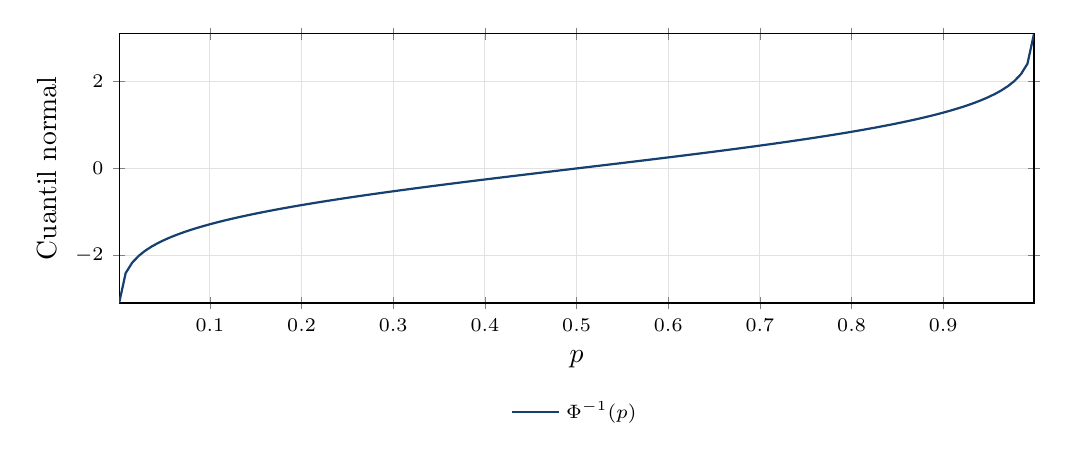
\begin{tikzpicture}\begin{axis}[base,axis lines=box,grid=major,minor tick num=0,width=13.2cm,height=5.0cm,xlabel={$p$},ylabel={Cuantil normal},legend style={at={(0.5,-0.32)},anchor=north,legend columns=2,font=\scriptsize,draw=none,fill=white}]
\addplot[thick,azul,] coordinates {(0.001,-3.090232306) (0.008128571429,-2.403090966) (0.01525714286,-2.163349797) (0.02238571429,-2.006795628) (0.02951428571,-1.887980477) (0.03664285714,-1.791047242) (0.04377142857,-1.708504041) (0.0509,-1.636189181) (0.05802857143,-1.571540551) (0.06515714286,-1.512863694) (0.07228571429,-1.458977035) (0.07941428571,-1.40902231) (0.08654285714,-1.362355519) (0.09367142857,-1.318480474) (0.1008,-1.277006365) (0.1079285714,-1.237619601) (0.1150571429,-1.200064515) (0.1221857143,-1.164129763) (0.1293142857,-1.129638523) (0.1364428571,-1.096441264) (0.1435714286,-1.064410328) (0.1507,-1.0334358) (0.1578285714,-1.003422313) (0.1649571429,-0.9742865404) (0.1720857143,-0.9459552163) (0.1792142857,-0.9183635412) (0.1863428571,-0.8914538969) (0.1934714286,-0.8651747953) (0.2006,-0.8394800138) (0.2077285714,-0.8143278786) (0.2148571429,-0.7896806653) (0.2219857143,-0.7655040956) (0.2291142857,-0.7417669116) (0.2362428571,-0.7184405134) (0.2433714286,-0.6954986497) (0.2505,-0.6729171513) (0.2576285714,-0.6506737017) (0.2647571429,-0.6287476372) (0.2718857143,-0.6071197735) (0.2790142857,-0.5857722541) (0.2861428571,-0.5646884167) (0.2932714286,-0.5438526755) (0.3004,-0.5232504179) (0.3075285714,-0.5028679117) (0.3146571429,-0.4826922234) (0.3217857143,-0.462711145) (0.3289142857,-0.442913128) (0.3360428571,-0.4232872243) (0.3431714286,-0.4038230338) (0.3503,-0.3845106553) (0.3574285714,-0.3653406436) (0.3645571429,-0.3463039695) (0.3716857143,-0.327391984) (0.3788142857,-0.3085963846) (0.3859428571,-0.2899091855) (0.3930714286,-0.2713226894) (0.4002,-0.2528294617) (0.4073285714,-0.2344223066) (0.4144571429,-0.2160942448) (0.4215857143,-0.1978384926) (0.4287142857,-0.1796484428) (0.4358428571,-0.1615176461) (0.4429714286,-0.1434397936) (0.4501,-0.1254087011) (0.4572285714,-0.1074182929) (0.4643571429,-0.08946258682) (0.4714857143,-0.07153568023) (0.4786142857,-0.05363173574) (0.4857428571,-0.03574496785) (0.4928714286,-0.01786962969) (0.5,0) (0.5071285714,0.01786962969) (0.5142571429,0.03574496785) (0.5213857143,0.05363173574) (0.5285142857,0.07153568023) (0.5356428571,0.08946258682) (0.5427714286,0.1074182929) (0.5499,0.1254087011) (0.5570285714,0.1434397936) (0.5641571429,0.1615176461) (0.5712857143,0.1796484428) (0.5784142857,0.1978384926) (0.5855428571,0.2160942448) (0.5926714286,0.2344223066) (0.5998,0.2528294617) (0.6069285714,0.2713226894) (0.6140571429,0.2899091855) (0.6211857143,0.3085963846) (0.6283142857,0.327391984) (0.6354428571,0.3463039695) (0.6425714286,0.3653406436) (0.6497,0.3845106553) (0.6568285714,0.4038230338) (0.6639571429,0.4232872243) (0.6710857143,0.442913128) (0.6782142857,0.462711145) (0.6853428571,0.4826922234) (0.6924714286,0.5028679117) (0.6996,0.5232504179) (0.7067285714,0.5438526755) (0.7138571429,0.5646884167) (0.7209857143,0.5857722541) (0.7281142857,0.6071197735) (0.7352428571,0.6287476372) (0.7423714286,0.6506737017) (0.7495,0.6729171513) (0.7566285714,0.6954986497) (0.7637571429,0.7184405134) (0.7708857143,0.7417669116) (0.7780142857,0.7655040956) (0.7851428571,0.7896806653) (0.7922714286,0.8143278786) (0.7994,0.8394800138) (0.8065285714,0.8651747953) (0.8136571429,0.8914538969) (0.8207857143,0.9183635412) (0.8279142857,0.9459552163) (0.8350428571,0.9742865404) (0.8421714286,1.003422313) (0.8493,1.0334358) (0.8564285714,1.064410328) (0.8635571429,1.096441264) (0.8706857143,1.129638523) (0.8778142857,1.164129763) (0.8849428571,1.200064515) (0.8920714286,1.237619601) (0.8992,1.277006365) (0.9063285714,1.318480474) (0.9134571429,1.362355519) (0.9205857143,1.40902231) (0.9277142857,1.458977035) (0.9348428571,1.512863694) (0.9419714286,1.571540551) (0.9491,1.636189181) (0.9562285714,1.708504041) (0.9633571429,1.791047242) (0.9704857143,1.887980477) (0.9776142857,2.006795628) (0.9847428571,2.163349797) (0.9918714286,2.403090966) (0.999,3.090232306)};
\addlegendentry{$\Phi^{-1}(p)$}
\end{axis}\end{tikzpicture}
\caption{Invertir una CDF cambia la sensibilidad: el cuantil se vuelve más empinado en extremos donde la densidad es pequeña.}\label{fig:cdf-21}\end{figure}

\section{Inicios centrales y AS 241}
Cerca de $p=1/2$, escribamos $u=p-1/2$. Como
$\Phi(x)-1/2=\ph(0)(x-x^3/6+\cdots)$, la inversión de series comienza
\[
x=\sqrt{2\pi}\,u+\frac{(2\pi)^{3/2}}6u^3+\cdots.
\]
Se determina cada coeficiente sustituyendo en la serie directa y comparando potencias. La simetría del cuantil exige una serie impar en $u$.

El algoritmo AS 241 de Wichura usa aproximaciones racionales por regiones para cuantiles normales. La documentación actual consultada de R distingue esos aproximantes de desarrollos adicionales en colas logarítmicas. No es necesario integrar de nuevo en cada paso si el aproximante ya tiene precisión suficiente.

Un racional inicial combinado con una corrección Newton puede mejorar un diseño, pero cada corrección cuesta una evaluación de CDF y densidad y puede empeorar si esas salidas son menos precisas que el inicio.

\section{Inversión gamma: origen, transición y cola}
Para $p$ pequeño con forma $a$ fija,
\[
P(a,x)\sim x^a/\Gamma(a+1),\qquad
\log x_0=\frac{\log p+\log\Gamma(a+1)}a.
\]
Si $a$ es muy pequeño, $x_0$ puede ser menor que el mínimo representable. Se puede devolver un log-cuantil cuando la interfaz lo permite.

Para forma grande y probabilidades centrales, una aproximación de transformación cúbica es
\[
x_0=a\left(1-\frac1{9a}+\frac z{3\sqrt a}\right)^3,
\quad z=\Phi^{-1}(p).
\]
Se trata de un inicio asintótico, no de una identidad. Si la expresión interior es negativa, no se usa como cuantil gamma.

Para cola superior lejana, con $L=-\log q$,
\[
x_0\approx L+(a-1)\log L-\log\Gamma(a).
\]
El refinamiento usa $P$ o $Q$ directamente según la cola, y mantiene $x>0$.

\section{Inversión beta y de Fisher}
Cerca de cero,
\[
I_x(a,b)\sim\frac{x^a}{aB(a,b)},\qquad
\log x_0=\frac{\log p+\log a+\log B(a,b)}a.
\]
Cerca de uno se invierte $I_{1-x}(b,a)$ para la cola complementaria. Para parámetros centrales grandes, media, varianza y un cuantil normal ofrecen un inicio.

Una vez obtenido $z$ y su complemento $y$ para beta,
\[
w=\frac ba\frac zy,\qquad
\log w=\log b-\log a+\log z-\log y.
\]
Si $y$ no es representable, el cuantil F puede desbordar mientras su logaritmo sigue siendo finito. Una interfaz que guarda solo $z=1$ pierde ese cuantil finito de gran magnitud.

Para t, se usa la reducción beta y el signo de $p-1/2$. En todas las distribuciones, los extremos $p=0,1$ se tratan según el soporte y no se pasan a Newton como raíces interiores.

\section{Condición del cuantil y cotas de probabilidad}
Sea $x_p=F^{-1}(p)$, con densidad positiva. Para pequeñas perturbaciones,
\[
\Delta x_p\approx\frac{\Delta p}{f(x_p)}.
\]
Si la entrada se expresa como $\ell=\log p$, entonces
$\dd x_p/\dd\ell=p/f(x_p)$. Para una cola superior $q$, la derivada respecto de $\log q$ es $-q/f$, frecuentemente de tamaño moderado.

Si conocemos $p\in[p_-,p_+]$ y $F$ es creciente,
\[
F^{-1}(p_-)\le x_p\le F^{-1}(p_+).
\]
La monotonía transforma un intervalo de probabilidades en uno de cuantiles, aunque el intervalo puede ser amplio en cola.

Evaluar $F(\widehat x)\approx p$ es una prueba de consistencia, no una prueba independiente si ambos algoritmos usan la misma aproximación. Se compara además con una ruta distinta o un encierro riguroso.

\section{Un algoritmo común con interfaces distintas}
La estructura raíz--intervalo--corrección es compartida:
\begin{lstlisting}
validate parameters and probability representation
choose lower or upper tail, ordinary or log scale
construct an interval containing the quantile
choose an initial point from a regional approximation
repeat:
    evaluate requested tail and a stable density ratio
    propose Newton or Halley
    replace unsafe proposal by bisection
    update the containing interval
stop only when the requested accuracy is supported
\end{lstlisting}
Lo que cambia es la función especial, el soporte, el inicio y los cocientes. Abstraer la estructura no elimina el análisis específico de normal, gamma y beta. Una tolerancia universal aplicada sin considerar escala y condición produce resultados desiguales.


\parte{XII. Varias dimensiones: regiones, matrices y azar}
\section{La normal multivariada desde una transformación}
Sea $Z=(Z_1,\ldots,Z_d)\T$ con componentes normales estándar independientes, y $X=\mu+LZ$, donde $L$ es invertible. Entonces
\[
\E X=\mu,\qquad \Cov(X)=LL\T=\Sigma.
\]
La igualdad de covarianza se deduce expandiendo $\E[(X-\mu)(X-\mu)\T]$ y usando $\E ZZ\T=I$. Si $\Sigma$ es definida positiva, Cholesky proporciona un $L$ triangular con diagonal positiva.

El cambio de variable tiene jacobiano $|\det L|$. La densidad es
\[
f_X(x)=\frac{\exp[-(x-\mu)\T\Sigma^{-1}(x-\mu)/2]}
{(2\pi)^{d/2}\sqrt{\det\Sigma}}.
\]
La forma cuadrática mide distancia de Mahalanobis. La CDF
$\Pr(X_1\le b_1,\ldots,X_d\le b_d)$ integra sobre un ortante; esa región no se convierte, en general, en un producto independiente al aplicar $L^{-1}$.

Si $\Sigma$ es singular, la distribución vive en un subespacio y no tiene esta densidad respecto de volumen en $\R^d$. Se reduce el rango o se trabaja directamente con una transformación rectangular.

\section{Condicionamiento bivariado}
Para normales estándar $X,Y$ con correlación $\rho$, $|\rho|<1$, podemos escribir
$Y=\rho X+\sqrt{1-\rho^2}Z$, con $Z$ independiente. Entonces
\[
\Phi_2(a,b;\rho)=\int_{-\infty}^a
\ph(x)\Phi\left(\frac{b-\rho x}{\sqrt{1-\rho^2}}\right)\dd x.
\]
El integrando es una densidad por una CDF condicional. La integral bidimensional se reduce a una dimensión.

Para $\rho=0$, factoriza en $\Phi(a)\Phi(b)$. Para $\rho\to1$, los dos valores se vuelven casi iguales y el límite es $\Phi(\min(a,b))$. Para $\rho\to-1$, el evento depende de un intervalo para una sola normal. Cerca de estos límites, el denominador pequeño puede crear una transición muy estrecha: la cuadratura necesita transformación o tratamiento límite.

\section{Una probabilidad exacta con correlación}
En $a=b=0$, existe la fórmula
\[
\Phi_2(0,0;\rho)=\frac14+\frac{\arcsin\rho}{2\pi}.
\]
Una deducción verifica que la derivada de la densidad bivariada respecto de $\rho$ coincide con su derivada mixta respecto de los argumentos. Integrar esa derivada sobre el ortante y usar que los términos de borde en infinito desaparecen da
\[
\frac{\partial}{\partial\rho}\Phi_2(0,0;\rho)
=\frac1{2\pi\sqrt{1-\rho^2}}.
\]
Integrar desde $\rho=0$, donde la probabilidad es $1/4$, produce la fórmula.

Para $\rho=1/2$, $\arcsin(1/2)=\pi/6$ y la probabilidad es $1/3$. Esta identidad es una referencia exacta valiosa para validar integración condicional, simulación y transformaciones de Cholesky.






\begin{figure}[htbp]\centering
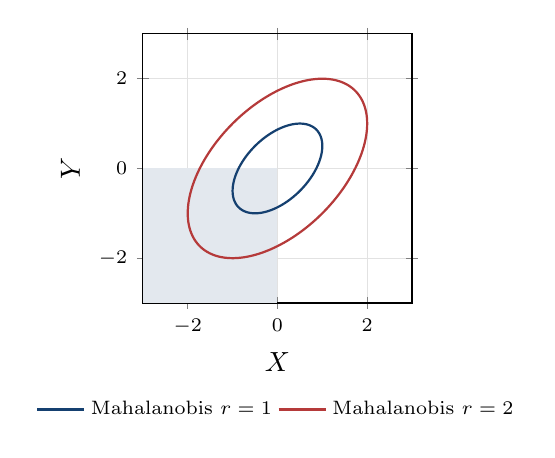
\begin{tikzpicture}\begin{axis}[base,axis lines=box,grid=major,minor tick num=0,width=13.2cm,height=5.0cm,xlabel={$X$},ylabel={$Y$},axis equal image,xmin=-3,xmax=3,ymin=-3,ymax=3,legend style={at={(0.5,-0.32)},anchor=north,legend columns=2,font=\scriptsize,draw=none,fill=white}]
\fill[azul!12] (axis cs:-3,-3) rectangle (axis cs:0,0);
\addplot[thick,azul,] coordinates {(1,0.5) (0.9992290362,0.5336145159) (0.9969173337,0.5664062369) (0.993068457,0.5983246006) (0.9876883406,0.629320391) (0.9807852804,0.6593458151) (0.9723699204,0.6883545757) (0.9624552365,0.7163019434) (0.9510565163,0.7431448255) (0.9381913359,0.7688418321) (0.9238795325,0.7933533403) (0.9081431738,0.8166415552) (0.8910065242,0.8386705679) (0.8724960071,0.8594064115) (0.8526401644,0.8788171127) (0.8314696123,0.8968727415) (0.8090169944,0.9135454576) (0.7853169309,0.9288095529) (0.7604059656,0.9426414911) (0.7343225094,0.9550199445) (0.7071067812,0.9659258263) (0.6788007455,0.9753423205) (0.6494480483,0.9832549076) (0.6190939493,0.9896513868) (0.5877852523,0.9945218954) (0.555570233,0.9978589232) (0.5224985647,0.999657325) (0.4886212415,0.9999143276) (0.4539904997,0.9986295348) (0.4186597375,0.9958049276) (0.3826834324,0.9914448614) (0.3461170571,0.9855560591) (0.3090169944,0.9781476007) (0.2714404499,0.9692309097) (0.2334453639,0.9588197349) (0.195090322,0.9469301295) (0.156434465,0.9335804265) (0.1175373975,0.9187912101) (0.07845909573,0.9025852843) (0.03925981576,0.8849876375) (6.123233996e-17,0.8660254038) (-0.03925981576,0.8457278217) (-0.07845909573,0.8241261886) (-0.1175373975,0.8012538127) (-0.156434465,0.7771459615) (-0.195090322,0.7518398075) (-0.2334453639,0.725374371) (-0.2714404499,0.6977904598) (-0.3090169944,0.6691306064) (-0.3461170571,0.639439002) (-0.3826834324,0.608761429) (-0.4186597375,0.57714519) (-0.4539904997,0.544639035) (-0.4886212415,0.5112930861) (-0.5224985647,0.4771587603) (-0.555570233,0.4422886902) (-0.5877852523,0.4067366431) (-0.6190939493,0.3705574375) (-0.6494480483,0.3338068592) (-0.6788007455,0.296541575) (-0.7071067812,0.2588190451) (-0.7343225094,0.220697435) (-0.7604059656,0.1822355255) (-0.7853169309,0.143492622) (-0.8090169944,0.1045284633) (-0.8314696123,0.06540312923) (-0.8526401644,0.02617694831) (-0.8724960071,-0.01308959557) (-0.8910065242,-0.05233595624) (-0.9081431738,-0.09150161866) (-0.9238795325,-0.1305261922) (-0.9381913359,-0.1693495038) (-0.9510565163,-0.2079116908) (-0.9624552365,-0.246153293) (-0.9723699204,-0.2840153447) (-0.9807852804,-0.3214394653) (-0.9876883406,-0.3583679495) (-0.993068457,-0.3947438564) (-0.9969173337,-0.4305110968) (-0.9992290362,-0.4656145203) (-1,-0.5) (-0.9992290362,-0.5336145159) (-0.9969173337,-0.5664062369) (-0.993068457,-0.5983246006) (-0.9876883406,-0.629320391) (-0.9807852804,-0.6593458151) (-0.9723699204,-0.6883545757) (-0.9624552365,-0.7163019434) (-0.9510565163,-0.7431448255) (-0.9381913359,-0.7688418321) (-0.9238795325,-0.7933533403) (-0.9081431738,-0.8166415552) (-0.8910065242,-0.8386705679) (-0.8724960071,-0.8594064115) (-0.8526401644,-0.8788171127) (-0.8314696123,-0.8968727415) (-0.8090169944,-0.9135454576) (-0.7853169309,-0.9288095529) (-0.7604059656,-0.9426414911) (-0.7343225094,-0.9550199445) (-0.7071067812,-0.9659258263) (-0.6788007455,-0.9753423205) (-0.6494480483,-0.9832549076) (-0.6190939493,-0.9896513868) (-0.5877852523,-0.9945218954) (-0.555570233,-0.9978589232) (-0.5224985647,-0.999657325) (-0.4886212415,-0.9999143276) (-0.4539904997,-0.9986295348) (-0.4186597375,-0.9958049276) (-0.3826834324,-0.9914448614) (-0.3461170571,-0.9855560591) (-0.3090169944,-0.9781476007) (-0.2714404499,-0.9692309097) (-0.2334453639,-0.9588197349) (-0.195090322,-0.9469301295) (-0.156434465,-0.9335804265) (-0.1175373975,-0.9187912101) (-0.07845909573,-0.9025852843) (-0.03925981576,-0.8849876375) (-1.836970199e-16,-0.8660254038) (0.03925981576,-0.8457278217) (0.07845909573,-0.8241261886) (0.1175373975,-0.8012538127) (0.156434465,-0.7771459615) (0.195090322,-0.7518398075) (0.2334453639,-0.725374371) (0.2714404499,-0.6977904598) (0.3090169944,-0.6691306064) (0.3461170571,-0.639439002) (0.3826834324,-0.608761429) (0.4186597375,-0.57714519) (0.4539904997,-0.544639035) (0.4886212415,-0.5112930861) (0.5224985647,-0.4771587603) (0.555570233,-0.4422886902) (0.5877852523,-0.4067366431) (0.6190939493,-0.3705574375) (0.6494480483,-0.3338068592) (0.6788007455,-0.296541575) (0.7071067812,-0.2588190451) (0.7343225094,-0.220697435) (0.7604059656,-0.1822355255) (0.7853169309,-0.143492622) (0.8090169944,-0.1045284633) (0.8314696123,-0.06540312923) (0.8526401644,-0.02617694831) (0.8724960071,0.01308959557) (0.8910065242,0.05233595624) (0.9081431738,0.09150161866) (0.9238795325,0.1305261922) (0.9381913359,0.1693495038) (0.9510565163,0.2079116908) (0.9624552365,0.246153293) (0.9723699204,0.2840153447) (0.9807852804,0.3214394653) (0.9876883406,0.3583679495) (0.993068457,0.3947438564) (0.9969173337,0.4305110968) (0.9992290362,0.4656145203) (1,0.5)};
\addlegendentry{Mahalanobis $r=1$}
\addplot[thick,rojo,] coordinates {(2,1) (1.998458072,1.067229032) (1.993834667,1.132812474) (1.986136914,1.196649201) (1.975376681,1.258640782) (1.961570561,1.31869163) (1.944739841,1.376709151) (1.924910473,1.432603887) (1.902113033,1.486289651) (1.876382672,1.537683664) (1.847759065,1.586706681) (1.816286348,1.63328311) (1.782013048,1.677341136) (1.744992014,1.718812823) (1.705280329,1.757634225) (1.662939225,1.793745483) (1.618033989,1.827090915) (1.570633862,1.857619106) (1.520811931,1.885282982) (1.468645019,1.910039889) (1.414213562,1.931851653) (1.357601491,1.950684641) (1.298896097,1.966509815) (1.238187899,1.979302774) (1.175570505,1.989043791) (1.111140466,1.995717846) (1.044997129,1.99931465) (0.977242483,1.999828655) (0.9079809995,1.99725907) (0.8373194751,1.991609855) (0.7653668647,1.982889723) (0.6922341142,1.971112118) (0.6180339887,1.956295201) (0.5428808997,1.938461819) (0.4668907277,1.91763947) (0.390180644,1.893860259) (0.3128689301,1.867160853) (0.2350747949,1.83758242) (0.1569181915,1.805170569) (0.07851963152,1.769975275) (1.224646799e-16,1.732050808) (-0.07851963152,1.691455643) (-0.1569181915,1.648252377) (-0.2350747949,1.602507625) (-0.3128689301,1.554291923) (-0.390180644,1.503679615) (-0.4668907277,1.450748742) (-0.5428808997,1.39558092) (-0.6180339887,1.338261213) (-0.6922341142,1.278878004) (-0.7653668647,1.217522858) (-0.8373194751,1.15429038) (-0.9079809995,1.08927807) (-0.977242483,1.022586172) (-1.044997129,0.9543175205) (-1.111140466,0.8845773804) (-1.175570505,0.8134732862) (-1.238187899,0.741114875) (-1.298896097,0.6676137185) (-1.357601491,0.59308315) (-1.414213562,0.5176380902) (-1.468645019,0.44139487) (-1.520811931,0.364471051) (-1.570633862,0.286985244) (-1.618033989,0.2090569265) (-1.662939225,0.1308062585) (-1.705280329,0.05235389662) (-1.744992014,-0.02617919114) (-1.782013048,-0.1046719125) (-1.816286348,-0.1830032373) (-1.847759065,-0.2610523844) (-1.876382672,-0.3386990077) (-1.902113033,-0.4158233816) (-1.924910473,-0.4923065861) (-1.944739841,-0.5680306894) (-1.961570561,-0.6428789306) (-1.975376681,-0.7167358991) (-1.986136914,-0.7894877128) (-1.993834667,-0.8610221936) (-1.998458072,-0.9312290407) (-2,-1) (-1.998458072,-1.067229032) (-1.993834667,-1.132812474) (-1.986136914,-1.196649201) (-1.975376681,-1.258640782) (-1.961570561,-1.31869163) (-1.944739841,-1.376709151) (-1.924910473,-1.432603887) (-1.902113033,-1.486289651) (-1.876382672,-1.537683664) (-1.847759065,-1.586706681) (-1.816286348,-1.63328311) (-1.782013048,-1.677341136) (-1.744992014,-1.718812823) (-1.705280329,-1.757634225) (-1.662939225,-1.793745483) (-1.618033989,-1.827090915) (-1.570633862,-1.857619106) (-1.520811931,-1.885282982) (-1.468645019,-1.910039889) (-1.414213562,-1.931851653) (-1.357601491,-1.950684641) (-1.298896097,-1.966509815) (-1.238187899,-1.979302774) (-1.175570505,-1.989043791) (-1.111140466,-1.995717846) (-1.044997129,-1.99931465) (-0.977242483,-1.999828655) (-0.9079809995,-1.99725907) (-0.8373194751,-1.991609855) (-0.7653668647,-1.982889723) (-0.6922341142,-1.971112118) (-0.6180339887,-1.956295201) (-0.5428808997,-1.938461819) (-0.4668907277,-1.91763947) (-0.390180644,-1.893860259) (-0.3128689301,-1.867160853) (-0.2350747949,-1.83758242) (-0.1569181915,-1.805170569) (-0.07851963152,-1.769975275) (-3.673940397e-16,-1.732050808) (0.07851963152,-1.691455643) (0.1569181915,-1.648252377) (0.2350747949,-1.602507625) (0.3128689301,-1.554291923) (0.390180644,-1.503679615) (0.4668907277,-1.450748742) (0.5428808997,-1.39558092) (0.6180339887,-1.338261213) (0.6922341142,-1.278878004) (0.7653668647,-1.217522858) (0.8373194751,-1.15429038) (0.9079809995,-1.08927807) (0.977242483,-1.022586172) (1.044997129,-0.9543175205) (1.111140466,-0.8845773804) (1.175570505,-0.8134732862) (1.238187899,-0.741114875) (1.298896097,-0.6676137185) (1.357601491,-0.59308315) (1.414213562,-0.5176380902) (1.468645019,-0.44139487) (1.520811931,-0.364471051) (1.570633862,-0.286985244) (1.618033989,-0.2090569265) (1.662939225,-0.1308062585) (1.705280329,-0.05235389662) (1.744992014,0.02617919114) (1.782013048,0.1046719125) (1.816286348,0.1830032373) (1.847759065,0.2610523844) (1.876382672,0.3386990077) (1.902113033,0.4158233816) (1.924910473,0.4923065861) (1.944739841,0.5680306894) (1.961570561,0.6428789306) (1.975376681,0.7167358991) (1.986136914,0.7894877128) (1.993834667,0.8610221936) (1.998458072,0.9312290407) (2,1)};
\addlegendentry{Mahalanobis $r=2$}
\end{axis}\end{tikzpicture}
\caption{Normal bivariada con correlación $1/2$. La región sombreada corresponde a $X\le0,Y\le0$ y tiene probabilidad exacta $1/3$; las elipses son niveles de distancia, no fronteras de CDF.}\label{fig:cdf-22}\end{figure}

\section{Separación de variables en una región rectangular}
Queremos $\Pr(a_i<X_i\le b_i,\ i=1,\ldots,d)$. Con $X=\mu+LZ$ triangular, una vez fijados $z_1,\ldots,z_{i-1}$,
\[
\alpha_i=\frac{a_i-\mu_i-\sum_{j<i}L_{ij}z_j}{L_{ii}},
\quad
\beta_i=\frac{b_i-\mu_i-\sum_{j<i}L_{ij}z_j}{L_{ii}},
\]
\[
d_i=\Phi(\beta_i)-\Phi(\alpha_i).
\]
Introducimos $u_i\in(0,1)$ y
$z_i=\Phi^{-1}(\Phi(\alpha_i)+u_id_i)$.
Como $\ph(z_i)\dd z_i=d_i\dd u_i$,
\[
\Pr(a<X\le b)=\int_{[0,1]^d}\prod_{i=1}^dd_i(u_1,\ldots,u_{i-1})\dd u.
\]
El integrando no depende de $u_d$, por lo que una dimensión se integra gratuitamente.

La derivación procede por cambios condicionales sucesivos; no se sustituye una región dependiente por otra independiente sin jacobiano. Cada $d_i$ es una probabilidad de intervalo que necesita las operaciones estables deducidas para la normal univariada.

\section{Pesos pequeños, orden de variables y precisión}
Si muchos $d_i$ son pequeños, el producto puede subdesbordar. Guardamos
$\log w=\sum_i\log d_i$. Para promediar pesos de escalas distintas,
\[
\log\sum_j e^{\ell_j}
=M+\log\sum_j e^{\ell_j-M},\qquad M=\max_j\ell_j.
\]
Es la operación log-suma-exponencial.

Permutar las variables antes de Cholesky cambia las probabilidades condicionales y puede reducir la variación del integrando transformado. La probabilidad exacta no cambia; el costo y la varianza del estimador sí. La elección óptima depende de la región y la matriz.

Si un intervalo condicional tiene masa numéricamente cero, se necesita distinguir un evento realmente imposible de una masa que subdesbordó. El uso de log-colas y cuantiles de intervalos pequeños preserva información que una CDF ordinaria redondeada perdería.

\section{Monte Carlo: esperanza, varianza y covarianza}
Sea $U\sim\operatorname{Unif}([0,1]^d)$ y $g$ integrable. La integral es $I=\E g(U)$. Con $m$ muestras independientes,
\[
\widehat I_m=\frac1m\sum_{j=1}^mg(U_j),\quad
\E\widehat I_m=I,\quad
\Var(\widehat I_m)=\frac{\Var(g(U))}{m}.
\]
Para un vector de integrales $G(U)\in\R^k$,
\[
\Cov(\widehat I_m)=\frac1m\Sigma_G,\quad
\Sigma_G=\E[(G-\E G)(G-\E G)\T].
\]
Las covarianzas entre estimaciones importan si restamos CDF o calculamos sensibilidades usando las mismas muestras.

El estimador de $\Sigma_G$ es
$(m-1)^{-1}\sum(G_j-\overline G)(G_j-\overline G)\T$, bajo segundo momento finito. La matriz para la media divide además por $m$. Confundir ambas matrices multiplica errores estándar por $\sqrt m$.

\section{Una CDF rara y el costo relativo}
Para un indicador de evento con probabilidad $p$,
\[
\Var(\widehat p)=\frac{p(1-p)}m,\qquad
\frac{\operatorname{sd}(\widehat p)}p
=\sqrt{\frac{1-p}{mp}}.
\]
Si $p=10^{-8}$ y pedimos error estándar relativo de $1\%$, necesitamos aproximadamente $10^{12}$ muestras. Dimensión moderada no evita la dificultad de rareza.

Un intervalo normal aproximado basado en el teorema central del límite requiere un régimen adecuado; si se observan cero éxitos, no se concluye que $p=0$. Para indicadores existen cotas binomiales y concentraciones específicas, pero una media de pesos de importancia no tiene automáticamente distribución binomial.

La integración determinista de una cola univariada es mucho más eficiente que simularla sin transformación. Monte Carlo se vuelve atractivo cuando la dimensión o geometría impiden una cuadratura sencilla.

\section{Muestreo de importancia para la cola normal}
Para estimar $p=\Q(b)$, muestreamos $X\sim N(\theta,1)$. El cociente de densidades es
\[
\frac{\ph(x)}{\ph(x-\theta)}
=\exp(-\theta x+\theta^2/2).
\]
El estimador individual
$Y=\ind_{\{X>b\}}\exp(-\theta X+\theta^2/2)$
es insesgado, porque multiplicar por la densidad propuesta recupera la original.

Su segundo momento exacto es
\[
\E_\theta Y^2=e^{\theta^2}\Q(b+\theta),
\quad \Var_\theta Y=e^{\theta^2}\Q(b+\theta)-\Q(b)^2.
\]
Se deduce completando el cuadrado en la integral de $f^2/g$. Con $\theta=b$, las muestras se concentran cerca de la frontera rara. La razón del segundo momento a $p^2$ crece solo proporcionalmente a $b$ en cola, en vez de como $1/p$.

El cálculo de los pesos y de esta razón debe hacerse en logaritmos para $b$ grande. Una propuesta que no cubre todo el soporte del evento puede producir un estimador sesgado; aquí la normal desplazada conserva soporte completo.






\begin{figure}[htbp]\centering
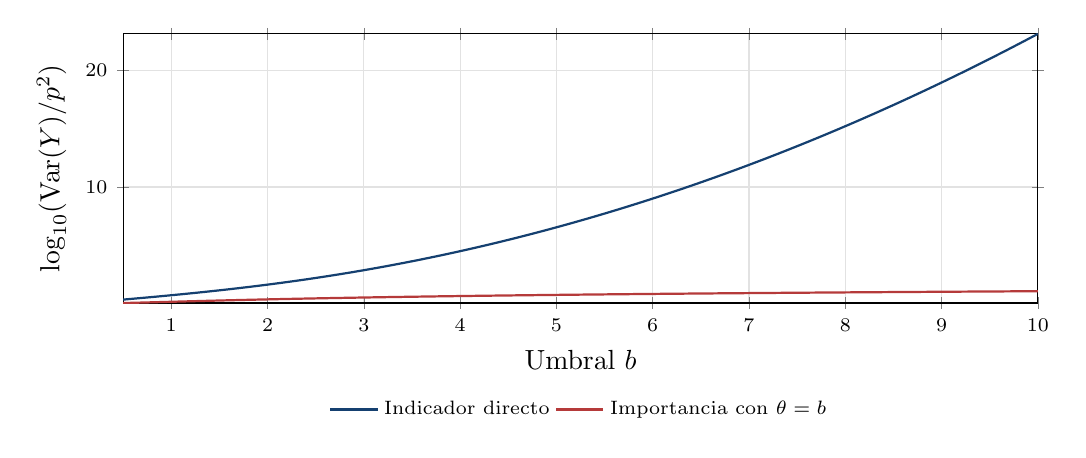
\begin{tikzpicture}\begin{axis}[base,axis lines=box,grid=major,minor tick num=0,width=13.2cm,height=5.0cm,xlabel={Umbral $b$},ylabel={$\log_{10}(\operatorname{Var}(Y)/p^2)$},legend style={at={(0.5,-0.32)},anchor=north,legend columns=2,font=\scriptsize,draw=none,fill=white}]
\addplot[thick,azul,] coordinates {(0.5,0.350460597) (0.5791666667,0.4075103341) (0.6583333333,0.4652458696) (0.7375,0.5237601209) (0.8166666667,0.5831455116) (0.8958333333,0.643493816) (0.975,0.7048959766) (1.054166667,0.7674418974) (1.133333333,0.8312202144) (1.2125,0.8963180477) (1.291666667,0.962820738) (1.370833333,1.030811574) (1.45,1.100371515) (1.529166667,1.171578922) (1.608333333,1.244509291) (1.6875,1.319235011) (1.766666667,1.395825146) (1.845833333,1.474345242) (1.925,1.554857181) (2.004166667,1.637419064) (2.083333333,1.722085145) (2.1625,1.808905809) (2.241666667,1.897927592) (2.320833333,1.989193249) (2.4,2.082741854) (2.479166667,2.178608942) (2.558333333,2.276826678) (2.6375,2.377424054) (2.716666667,2.480427098) (2.795833333,2.585859102) (2.875,2.69374085) (2.954166667,2.80409085) (3.033333333,2.916925563) (3.1125,3.032259621) (3.191666667,3.150106032) (3.270833333,3.270476377) (3.35,3.393380988) (3.429166667,3.518829106) (3.508333333,3.646829031) (3.5875,3.777388247) (3.666666667,3.910513538) (3.745833333,4.046211084) (3.825,4.184486545) (3.904166667,4.325345135) (3.983333333,4.468791684) (4.0625,4.614830687) (4.141666667,4.763466348) (4.220833333,4.914702619) (4.3,5.068543228) (4.379166667,5.224991702) (4.458333333,5.384051392) (4.5375,5.545725488) (4.616666667,5.710017034) (4.695833333,5.876928941) (4.775,6.046463997) (4.854166667,6.218624873) (4.933333333,6.393414136) (5.0125,6.570834253) (5.091666667,6.750887595) (5.170833333,6.933576445) (5.25,7.118903003) (5.329166667,7.306869388) (5.408333333,7.497477643) (5.4875,7.690729738) (5.566666667,7.886627576) (5.645833333,8.085172993) (5.725,8.286367761) (5.804166667,8.490213595) (5.883333333,8.69671215) (5.9625,8.905865026) (6.041666667,9.117673771) (6.120833333,9.332139883) (6.2,9.54926481) (6.279166667,9.769049955) (6.358333333,9.991496676) (6.4375,10.21660629) (6.516666667,10.44438007) (6.595833333,10.67481925) (6.675,10.90792502) (6.754166667,11.14369856) (6.833333333,11.38214098) (6.9125,11.62325337) (6.991666667,11.8670368) (7.070833333,12.1134923) (7.15,12.36262086) (7.229166667,12.61442345) (7.308333333,12.86890102) (7.3875,13.12605447) (7.466666667,13.38588471) (7.545833333,13.6483926) (7.625,13.91357897) (7.704166667,14.18144464) (7.783333333,14.45199042) (7.8625,14.72521707) (7.941666667,15.00112534) (8.020833333,15.27971598) (8.1,15.56098969) (8.179166667,15.84494717) (8.258333333,16.13158909) (8.3375,16.42091613) (8.416666667,16.71292891) (8.495833333,17.00762807) (8.575,17.30501421) (8.654166667,17.60508793) (8.733333333,17.90784982) (8.8125,18.21330044) (8.891666667,18.52144034) (8.970833333,18.83227005) (9.05,19.14579012) (9.129166667,19.46200105) (9.208333333,19.78090333) (9.2875,20.10249747) (9.366666667,20.42678394) (9.445833333,20.75376321) (9.525,21.08343572) (9.604166667,21.41580194) (9.683333333,21.75086229) (9.7625,22.0886172) (9.841666667,22.42906709) (9.920833333,22.77221235) (10,23.11805341)};
\addlegendentry{Indicador directo}
\addplot[thick,rojo,] coordinates {(0.5,0.05690163038) (0.5791666667,0.07236230123) (0.6583333333,0.08863672535) (0.7375,0.1054948909) (0.8166666667,0.1227464789) (0.8958333333,0.1402355426) (0.975,0.1578354491) (1.054166667,0.1754442699) (1.133333333,0.192980702) (1.2125,0.2103805353) (1.291666667,0.2275936395) (1.370833333,0.2445814241) (1.45,0.2613147158) (1.529166667,0.2777719968) (1.608333333,0.2939379493) (1.6875,0.3098022578) (1.766666667,0.3253586269) (1.845833333,0.3406039764) (1.925,0.3555377846) (2.004166667,0.3701615516) (2.083333333,0.3844783626) (2.1625,0.3984925323) (2.241666667,0.4122093158) (2.320833333,0.4256346743) (2.4,0.4387750849) (2.479166667,0.4516373875) (2.558333333,0.4642286609) (2.6375,0.4765561236) (2.716666667,0.488627054) (2.795833333,0.5004487275) (2.875,0.5120283666) (2.954166667,0.5233731017) (3.033333333,0.5344899411) (3.1125,0.5453857475) (3.191666667,0.5560672216) (3.270833333,0.5665408892) (3.35,0.5768130928) (3.429166667,0.5868899865) (3.508333333,0.596777533) (3.5875,0.6064815024) (3.666666667,0.6160074736) (3.745833333,0.625360836) (3.825,0.6345467925) (3.904166667,0.6435703633) (3.983333333,0.6524363903) (4.0625,0.6611495419) (4.141666667,0.6697143179) (4.220833333,0.6781350551) (4.3,0.6864159322) (4.379166667,0.6945609758) (4.458333333,0.7025740653) (4.5375,0.7104589388) (4.616666667,0.718219198) (4.695833333,0.7258583135) (4.775,0.7333796303) (4.854166667,0.740786372) (4.933333333,0.7480816462) (5.0125,0.7552684492) (5.091666667,0.76234967) (5.170833333,0.7693280949) (5.25,0.7762064121) (5.329166667,0.7829872148) (5.408333333,0.7896730059) (5.4875,0.7962662013) (5.566666667,0.8027691334) (5.645833333,0.8091840547) (5.725,0.8155131411) (5.804166667,0.8217584947) (5.883333333,0.8279221471) (5.9625,0.8340060621) (6.041666667,0.8400121383) (6.120833333,0.8459422121) (6.2,0.8517980598) (6.279166667,0.8575814003) (6.358333333,0.8632938971) (6.4375,0.8689371605) (6.516666667,0.87451275) (6.595833333,0.880022176) (6.675,0.8854669017) (6.754166667,0.890848345) (6.833333333,0.8961678804) (6.9125,0.9014268402) (6.991666667,0.9066265166) (7.070833333,0.9117681629) (7.15,0.916852995) (7.229166667,0.9218821932) (7.308333333,0.9268569026) (7.3875,0.9317782353) (7.466666667,0.9366472714) (7.545833333,0.9414650596) (7.625,0.946232619) (7.704166667,0.9509509401) (7.783333333,0.9556209853) (7.8625,0.9602436903) (7.941666667,0.9648199652) (8.020833333,0.9693506949) (8.1,0.9738367404) (8.179166667,0.9782789394) (8.258333333,0.9826781071) (8.3375,0.9870350371) (8.416666667,0.991350502) (8.495833333,0.9956252543) (8.575,0.9998600268) (8.654166667,1.004055533) (8.733333333,1.00821247) (8.8125,1.012331513) (8.891666667,1.016413326) (8.970833333,1.020458551) (9.05,1.024467816) (9.129166667,1.028441736) (9.208333333,1.032380906) (9.2875,1.03628591) (9.366666667,1.040157318) (9.445833333,1.043995684) (9.525,1.04780155) (9.604166667,1.051575446) (9.683333333,1.055317888) (9.7625,1.059029381) (9.841666667,1.062710419) (9.920833333,1.066361481) (10,1.06998304)};
\addlegendentry{Importancia con $\theta=b$}
\end{axis}\end{tikzpicture}
\caption{Varianza relativa por muestra al estimar una cola normal. Para $m$ muestras se divide por $m$. El desplazamiento de importancia reduce drásticamente la dificultad de rareza en este ejemplo.}\label{fig:cdf-23}\end{figure}

\section{Cuasi Monte Carlo y aleatorización}
Cuasi Monte Carlo usa puntos con distribución espacial uniforme de forma determinista. Bajo variación de Hardy--Krause finita, Koksma--Hlawka acota
\[
\left|\frac1m\sum_{j=1}^mg(u_j)-\int g\right|
\le V_{\rm HK}(g)D_m^*.
\]
La discrepancia $D_m^*$ mide irregularidad de puntos respecto de cajas ancladas. Un integrando con cuantiles inversos singulares en bordes puede no cumplir fácilmente las hipótesis; no se aplica la cota sin verificarlas.

Aleatorizaciones de secuencias de baja discrepancia permiten replicaciones independientes. Si tenemos $R$ replicaciones con estimaciones $I_r$, estimamos incertidumbre entre esas replicaciones, no tratando todos los puntos internos como muestras independientes.

La integración condicional suele suavizar indicadores y beneficiar estas técnicas. El comportamiento depende de dimensión efectiva y regularidad, no solo de la dimensión nominal.

\section{Mallas dispersas y diferencias tensoriales}
Sean reglas unidimensionales anidadas $Q_\ell$ y $\Delta_\ell=Q_\ell-Q_{\ell-1}$, con $Q_0=0$. Una construcción de Smolyak suma
\[
A_q=\sum_{\substack{\ell_i\ge1\\\ell_1+\cdots+\ell_d\le q}}
\Delta_{\ell_1}\otimes\cdots\otimes\Delta_{\ell_d}.
\]
Selecciona incrementos de nivel total limitado en vez de todas las combinaciones hasta un nivel máximo. Para constantes, los incrementos superiores pueden anularse y muchas combinaciones no son necesarias.

La ventaja exige cierta regularidad mixta y decaimiento de contribuciones altas. Una discontinuidad de indicador o un fuerte acoplamiento puede limitarla. Los coeficientes combinados pueden ser negativos, por lo que una integral de densidad no conserva automáticamente positividad.

La cuadratura tensorial, las mallas dispersas y QMC ofrecen compromisos diferentes entre estructura, determinismo e incertidumbre.

\section{Gradientes de una probabilidad multivariada}
Para una región fija $\mathcal R$ y parámetros $\theta$ de una densidad suave,
\[
\partial_\theta\Pr_\theta(X\in\mathcal R)
=\int_{\mathcal R}\partial_\theta f_\theta(x)\dd x
=\E_\theta[\ind_{\mathcal R}(X)\,\partial_\theta\log f_\theta(X)],
\]
si se justifica diferenciar bajo la integral. La función $\partial_\theta\log f$ es una puntuación. Para media normal,
\[
\nabla_\mu\log f_\mu(x)=\Sigma^{-1}(x-\mu).
\]
Un vector de estimadores de gradientes tiene una matriz de covarianza que se calcula igual que para cualquier media vectorial.

Si la región también depende del parámetro, aparecen términos de frontera; la fórmula de puntuación sola no los incluye. Diferenciación automática de un algoritmo aproximado puede dar la derivada de ese algoritmo, no necesariamente una derivada exacta de la probabilidad objetivo.


\parte{XIII. Algoritmos actuales: adaptación, precisión y certificación}
\section{AAA: racionales en forma baricéntrica}
Elegimos puntos de soporte $z_1,\ldots,z_m$ y valores $f_j=f(z_j)$. La forma
\[
r(z)=\frac{\sum_{j=1}^m w_jf_j/(z-z_j)}
{\sum_{j=1}^m w_j/(z-z_j)}
\]
interpola en soportes cuando los pesos correspondientes son no nulos y el límite no degenera. Ahora $w_j$ son incógnitas adaptativas, no los pesos especiales que generan un polinomio Lagrange.

Para muestras restantes $Z_i$ con valores $F_i$, el residuo linealizado es
\[
F_i\sum_j\frac{w_j}{Z_i-z_j}
-\sum_j\frac{w_jf_j}{Z_i-z_j}
=\sum_j\frac{F_i-f_j}{Z_i-z_j}w_j.
\]
Definimos la matriz de Loewner
$L_{ij}=(F_i-f_j)/(Z_i-z_j)$. Buscamos $\norm w_2=1$ que minimice $\norm{Lw}_2$. Es el vector singular derecho de menor valor singular.

AAA elige de forma voraz el próximo soporte donde el error muestreado es mayor, reconstruye $L$ y repite. Esta es la conexión con SVD: un problema racional no lineal se construye mediante etapas lineales.

\section{Qué minimiza AAA y qué debe comprobarse}
El residual $Lw$ es el numerador de $F-r$ multiplicado por el denominador. Minimizarlo no equivale exactamente a minimizar $\max|F-r|$. El denominador puede variar mucho. AAA es una construcción adaptativa eficaz, pero no se debe denominar minimax certificado sin otra verificación.

Polos y ceros casi cancelados, llamados pares de Froissart, pueden aparecer por ruido o redondeo. Se examinan residuos y se elimina soporte o se reformula el aproximante cuando la cancelación produce un polo espurio cerca del dominio.

Las muestras no prueban ausencia de un error grande entre ellas. Para una CDF se comprueban además monotonía, rango $[0,1]$, cola y continuidad en fronteras. Aproximar una función escalada puede hacer el problema mucho más favorable.

El artículo AAA de Nakatsukasa, Sète y Trefethen se publicó en 2018 tras versiones preliminares anteriores; el hito histórico indicado en el libro se refiere a su publicación.

\section{Racional de datos y racional certificado}
Sea $r=p/q$, con $|q(x)|\ge d>0$ en el intervalo. Si coeficientes redondeados producen $\widetilde p,\widetilde q$ y $|\widetilde q|\ge\widetilde d>0$,
\[
\left|\frac pq-\frac{\widetilde p}{\widetilde q}\right|
\le\frac{|p-\widetilde p|}{d}
+\frac{|\widetilde p||q-\widetilde q|}{d\widetilde d}.
\]
Una cota de coeficientes en la base elegida permite acotar los numeradores de esta desigualdad. En Chebyshev, $|T_k|\le1$ hace la suma de errores de coeficiente especialmente simple en $[-1,1]$.

La derivada es
\[
r'=\frac{p'q-pq'}{q^2}.
\]
Si encerramos el polinomio $p'q-pq'$ como no negativo y probamos que $q$ no se anula, certificamos monotonía. Si además los extremos están dentro de $[0,1]$, el racional permanece en ese rango.

Certificar propiedades de distribución y certificar error respecto de la CDF verdadera son tareas distintas. Un racional creciente puede aproximar una CDF equivocada.

\section{Intervalos: operaciones y redondeo exterior}
Un intervalo $[a,b]$ representa todos los reales entre ambos extremos. Si $X=[a,b]$ y $Y=[c,d]$,
\[
X+Y=[a+c,b+d],\qquad X-Y=[a-d,b-c],
\]
\[
XY=[\min(ac,ad,bc,bd),\max(ac,ad,bc,bd)].
\]
La división requiere que $0\notin Y$. Para garantías en computadora, los extremos inferiores se redondean hacia abajo y los superiores hacia arriba. Calcularlos al más cercano no basta para afirmar encierro.

La dependencia ensancha intervalos: si $X=[-1,1]$, $X-X=[-2,2]$ por las reglas, aunque la expresión exacta $x-x$ sea cero. Reformular algebraicamente o usar modelos de Taylor reduce esa sobreestimación.

Si una integral tiene un intervalo de error que incluye cero, no significa que sea exactamente cero. Una certificación devuelve una región que contiene el resultado y cuya anchura se puede reducir con más trabajo o precisión.

\section{Aritmética de bolas}
Una bola real se escribe $c\pm r$. Para productos de $c\pm r$ y $d\pm s$, un radio válido alrededor de $cd$ es
\[
|c|s+|d|r+rs,
\]
más una cota de redondeo del centro. Es la desigualdad triangular aplicada a
$(c+\delta)(d+\eta)-cd=c\eta+d\delta+\delta\eta$.

Una bola permite propagar error de truncamiento, entrada y aritmética conjuntamente. Si el radio es mayor que el centro de una cola pequeña, no se tienen cifras relativas fiables aunque el intervalo absoluto sea corto.

Los trabajos de Johansson sobre Arb y cuadratura en aritmética de bolas muestran una vía de certificación arbitraria. Precisión ampliada y certificación son diferentes: cien dígitos calculados al más cercano no constituyen por sí mismos una cota de cien dígitos.

\section{Certificar una integral con Taylor local}
En una celda $[c-h,c+h]$, aproximamos $f$ por Taylor de grado $m$. Si $|f^{(m+1)}|\le M$ en la celda, entonces
\[
\left|\int_{c-h}^{c+h}(f-p_m)\dd x\right|
\le\frac{2Mh^{m+2}}{(m+1)!(m+2)}.
\]
La cota se obtiene integrando $M|x-c|^{m+1}/(m+1)!$. Los términos impares de $p_m$ integran cero y los pares se integran exactamente.

Partimos el intervalo y sumamos encierros. El dominio infinito añade una cota de cola. Una transformación puede facilitar la acotación de derivadas, pero hay que incluir jacobianos y posibles singularidades.

La certificación analítica con elipses o discos complejos puede producir cotas más eficientes. Su validez exige conocer un recinto libre de singularidades y una cota del integrando en él.

\section{Ecuaciones diferenciales de las CDF}
Las densidades conocidas generan ecuaciones:
\[
\Phi''(x)+x\Phi'(x)=0,
\]
\[
xP''(a,x)+(x+1-a)P'(a,x)=0,
\]
\[
x(1-x)I''_x(a,b)+[1-a+(a+b-2)x]I'_x(a,b)=0.
\]
La primera usa $\ph'=-x\ph$. La segunda y tercera se deducen diferenciando la log-densidad. Son ecuaciones de segundo orden con soluciones constantes además de la CDF; las condiciones iniciales o de borde seleccionan la solución correcta.

Podemos avanzar mediante Taylor, Runge--Kutta o métodos de alta precisión. El error de integración de la ecuación es un nuevo presupuesto. Estas ecuaciones también verifican residuales de aproximantes, pero un residual pequeño no garantiza error pequeño sin condiciones de borde y estabilidad del problema.

\section{Mills como ecuación y dirección estable}
Del cociente $R=\Q/\ph$ se obtiene
\[
R'(x)=xR(x)-1.
\]
Una perturbación $\delta R$ obedece la ecuación homogénea
$\delta R'=x\delta R$, por lo que
\[
\delta R(x)=\delta R(B)\exp[(x^2-B^2)/2].
\]
Avanzar desde cero hacia una cola grande amplifica el error exponencialmente. Integrar hacia atrás desde un $B$ grande atenúa el error de borde.

Un algoritmo puede iniciar $R(B)$ con una expansión asintótica encerrada y avanzar hacia la región central. Se debe contar además el error local del integrador, que se propaga con el mismo mecanismo. La elección de dirección viene del análisis de la ecuación, no solo de comodidad.

Esta deducción explica por qué ciertas recurrencias y ecuaciones especiales se calculan en dirección descendente: la solución deseada puede ser la componente mínima frente a una solución homogénea que crece.

\section{División binaria de series}
Si términos satisfacen $t_{k+1}=r_kt_k$, una suma finita se puede reorganizar por bloques. Para un bloque $[l,r)$ definimos
\[
P_{l,r}=\prod_{k=l}^{r-1}r_k,\quad
S_{l,r}=1+r_l+r_lr_{l+1}+\cdots+\prod_{k=l}^{r-2}r_k.
\]
Al dividir en $m$,
\[
P_{l,r}=P_{l,m}P_{m,r},\qquad
S_{l,r}=S_{l,m}+P_{l,m}S_{m,r}.
\]
La base de longitud uno es $P=r_l,S=1$. Una suma de los términos originales es $t_lS_{l,r}$.

Para razones racionales se pueden mantener numeradores y denominadores enteros y realizar divisiones al final. La estructura equilibrada aprovecha multiplicación rápida de enteros y reduce ciertas operaciones costosas en precisión alta. El costo depende del crecimiento de enteros, de la serie y de la precisión; no se presenta una aceleración universal sin esas condiciones.

\section{GPU, SIMD y muchos argumentos}
Un polinomio pequeño con Horner es favorable para evaluar grandes vectores de argumentos. Un algoritmo adaptativo con distinto número de iteraciones para cada entrada puede producir divergencia de ramas. Dividir previamente argumentos por región permite ejecutar rutinas homogéneas.

El rendimiento se mide junto a precisión: una aproximación de cinco cifras no se compara directamente con una de quince como si resolvieran el mismo encargo. Las instrucciones exponencial y logarítmica del dispositivo pueden tener garantías diferentes; la validación debe hacerse en la plataforma objetivo.

Precalcular coeficientes reduce costo por consulta. Si los parámetros $a,b$ cambian en cada elemento, el precálculo de una superficie racional en varios parámetros puede volverse grande. La adaptabilidad y la memoria forman otro compromiso.

\section{Cómo leer una biblioteca numérica actual}
La documentación consultada identifica algoritmos distintos para normal, cuantiles, gamma y beta. Una función pública puede cambiar su interior con el tiempo, por lo que una descripción debe referirse a una versión o documentación concreta.

Se examinan dominio de parámetros, colas, opción logarítmica, política de subdesbordamiento, error documentado y referencias. Una llamada con nombre familiar no prueba que se use siempre cuadratura de Gauss ni que todas las salidas posean error relativo uniforme.

Para aprendizaje, las implementaciones del laboratorio son transparentes y deliberadamente regionales. Se comparan con bibliotecas y con referencias de precisión ampliada; no se anuncian como sustitutos universales de rutinas que han recibido décadas de validación.


\parte{XIV. Más allá de una sola integral: fases, mezclas y otras funciones}
\section{Laplace: una integral dominada por un máximo}
Consideremos $I_n=\int_a^b e^{n\phi(t)}A(t)\dd t$, con un máximo interior único en $t_0$, $\phi'(t_0)=0$, $\phi''(t_0)<0$ y regularidad adecuada. Cerca del máximo,
\[
\phi(t)=\phi(t_0)-\frac{|\phi''(t_0)|}{2}(t-t_0)^2+\cdots.
\]
Con $s=\sqrt{n|\phi''(t_0)|}(t-t_0)$,
\[
I_n\sim e^{n\phi(t_0)}A(t_0)
\sqrt{\frac{2\pi}{n|\phi''(t_0)|}}.
\]
La parte fuera de una vecindad del máximo es exponencialmente menor si existe una separación positiva de fases. Dentro, Taylor y dominación controlan el cambio de escala.

Si el máximo está en un extremo, si $\phi''(t_0)=0$ o si dos máximos compiten, cambia la fórmula. Las expansiones uniformes estudian justamente transiciones donde una fórmula local ordinaria deja de ser uniforme.

\section{Deducir la primera corrección de Stirling}
En $\Gamma(a)=\int_0^\infty t^{a-1}e^{-t}\dd t$, pongamos $t=a(1+z/\sqrt a)$. Entonces
\[
\Gamma(a)=a^{a-1/2}e^{-a}\int_{-\sqrt a}^\infty
e^{-z^2/2}\frac{\exp[z^3/(3\sqrt a)-z^4/(4a)+\cdots]}
{1+z/\sqrt a}\dd z.
\]
En la región que contribuye al máximo, expandimos amplitud y exponencial. El término de orden $a^{-1/2}$ es $z^3/3-z$, impar, y su integral gaussiana es cero. El término de orden $a^{-1}$ es
\[
z^2-\frac7{12}z^4+\frac1{18}z^6.
\]
Los momentos normalizados son $1,3,15$ y su combinación es
$1-7(3)/12+15/18=1/12$. Por tanto
\[
\Gamma(a)\sim\sqrt{2\pi}a^{a-1/2}e^{-a}
\left(1+\frac1{12a}+O(a^{-2})\right).
\]
Tomar logaritmo produce el primer término $1/(12a)$ de log-gamma. No se expanden todas las $z$ hasta infinito sin control: una prueba completa divide región central y colas, y acota estas por la fase.

\section{Una transformación cúbica gamma explicada}
Para $X\sim\Gamma(a,1)$, $\E X=a$, $\Var X=a$. Sea $g(x)=x^{1/3}$. Taylor y el método delta dan
\[
\E g(X)\approx g(a)+\frac12g''(a)a
=a^{1/3}\left(1-\frac1{9a}\right),
\]
\[
\Var(g(X))\approx g'(a)^2a=\frac1{9a^{1/3}}.
\]
Dividiendo por $a^{1/3}$, $(X/a)^{1/3}$ tiene media aproximada $1-1/(9a)$ y desviación $1/(3\sqrt a)$. Aproximarlo por una normal y despejar $X$ produce el inicio cúbico usado en cuantiles.

La transformación reduce asimetría, pero los momentos aproximados no prueban normalidad exacta. El régimen es $a$ grande y fluctuaciones centrales; para una cola muy remota se utiliza una aproximación de fase.

\section{Punto de silla a partir de una función generadora}
La función generadora de cumulantes es $K(t)=\log\E e^{tX}$ donde existe. Para una normal estándar, $K(t)=t^2/2$; para gamma de forma $a$ y tasa uno,
\[
K(t)=-a\log(1-t),\quad t<1.
\]
El punto de silla para $x$ resuelve $K'(\widehat t)=x$. Definamos
\[
w=\sgn(\widehat t)\sqrt{2(\widehat tx-K(\widehat t))},
\qquad u=\widehat t\sqrt{K''(\widehat t)}.
\]
Una aproximación de CDF tipo Lugannani--Rice es
\[
F(x)\approx\Phi(w)+\ph(w)\left(\frac1w-\frac1u\right).
\]
Se obtiene de una inversión integral y una transformación de fase cuadrática; no es una identidad general ni una cota de error. Cerca de $\widehat t=0$ la diferencia tiene un límite removible que se evalúa por serie.

Para gamma, $\widehat t=1-a/x$, $w=\sqrt a\,\eta$ y $u=(x-a)/\sqrt a$. Recuperamos la corrección de la expansión uniforme. Para normal, $w=u=x$ y el término correctivo desaparece.

\section{Inversión de Fourier y una CDF sin densidad sencilla}

La identidad exponencial compleja permite escribir
\[
\phi_X(t)=\E[\cos(tX)]+i\E[\sin(tX)].
\]
Como $|e^{itX}|=1$, esta esperanza siempre existe, aunque $X$ no tenga media ni varianza. Para variables independientes,
$\phi_{X+Y}(t)=\phi_X(t)\phi_Y(t)$, porque la esperanza del producto de funciones acotadas independientes factoriza.

En una malla de $N$ puntos, la matriz
$D_{kj}=N^{-1/2}e^{-2\pi i kj/N}$ es un cambio de coordenadas ortonormal complejo. La identidad geométrica
\[
\sum_{j=0}^{N-1}e^{2\pi i(k-\ell)j/N}
=\begin{cases}N,&k=\ell,\\0,&k\ne\ell,\end{cases}
\]
para índices $0,\ldots,N-1$, demuestra $D^\ast D=I$, donde $\ast$ es transposición con conjugación. Una FFT calcula el mismo producto matricial aprovechando factorizaciones, en lugar de cambiar el problema exacto. Estas coordenadas espectrales explican la rapidez de convoluciones y reconstrucciones de distribuciones.

Sea $\phi_X(t)=\E e^{itX}$ la función característica. Bajo condiciones apropiadas, en un punto de continuidad,
\[
F(x)=\frac12-\frac1\pi\int_0^\infty
\frac{\operatorname{Im}(e^{-itx}\phi_X(t))}{t}\dd t.
\]
Esta es la fórmula de inversión de Gil--Pelaez. Cerca de $t=0$, el cociente tiene un límite relacionado con $\E X-x$ si el primer momento existe; no se evalúa como una división arbitraria por cero.

La integral es oscilatoria y posiblemente de convergencia condicional. Cortarla, discretizarla y estimar la cola requiere propiedades de $\phi_X$. Un método Gauss diseñado para un peso positivo no controla automáticamente cancelación de Fourier.

Para normal, $\phi_X(t)=e^{-t^2/2}$ y la inversión reproduce la CDF. Para sumas independientes, las características se multiplican, facilitando evaluar distribuciones cuyo integrando original es una convolución complicada.

\section{Convolución e integración de una CDF condicional}
Si $X,Y$ son independientes y $X$ tiene densidad,
\[
F_{X+Y}(s)=\int_\R f_X(t)F_Y(s-t)\dd t.
\]
La identidad proviene de condicionar en $X=t$. Derivando con dominación adecuada,
$f_{X+Y}(s)=\int f_X(t)f_Y(s-t)\dd t$. Para normales, la suma es normal con medias y varianzas sumadas, lo que ofrece un caso exacto de validación.

Una FFT calcula convoluciones discretizadas rápidamente, pero introduce truncamiento del dominio, paso de malla y convolución circular. Rellenar con ceros reduce aliasing circular; no corrige por sí solo error de cuadratura ni masas omitidas.

Para mezclas con escalas muy distintas, un solo paso uniforme puede no resolver la parte estrecha y simultáneamente cubrir la amplia. La adaptación o la separación de componentes preserva estructura.

\section{Chi cuadrado no central como mezcla Poisson}
Para una normal con media desplazada, completar el cuadrado da el generador de un cuadrado no central. Sumando componentes,
\[
M(t)=(1-2t)^{-\nu/2}
\exp\left(\frac{\lambda t}{1-2t}\right).
\]
Como $\lambda t/(1-2t)=(\lambda/2)[(1-2t)^{-1}-1]$,
\[
M(t)=e^{-\lambda/2}\sum_{j=0}^\infty
\frac{(\lambda/2)^j}{j!}(1-2t)^{-(\nu/2+j)}.
\]
Esto identifica una mezcla de chi cuadrados centrales con pesos Poisson:
\[
F_{\nu,\lambda}(x)=
\sum_{j=0}^\infty
e^{-\lambda/2}\frac{(\lambda/2)^j}{j!}
P(\nu/2+j,x/2).
\]
La identificación mediante generadores usa unicidad cuando existen en una vecindad de cero. La suma es positiva y permite reutilizar recurrencias gamma.

\section{F no central y una precaución de escala}
Si solo el numerador chi cuadrado es no central,
\[
F_{d_1,d_2,\lambda}(w)
=\sum_{j=0}^\infty p_j I_z(d_1/2+j,d_2/2),
\quad z=\frac{d_1w}{d_1w+d_2},
\]
con $p_j$ Poisson de media $\lambda/2$. El argumento $z$ conserva $d_1$ original porque el cociente se divide por esos grados originales.

No es simplemente $\sum p_jF_{d_1+2j,d_2}(w)$. La forma central equivalente evalúa
$F_{d_1+2j,d_2}(d_1w/(d_1+2j))$. Omitir esa escala calcula otra distribución.

Cuando la no centralidad es cero, solo queda $j=0$ y se recupera la F central. Esta comprobación y el límite $\lambda\downarrow0$ validan la estructura de mezcla.

\section{Sumar una mezcla alrededor de su modo}
Si $\theta=\lambda/2$ es grande, $p_0=e^{-\theta}$ puede subdesbordar. Comenzamos en $j_0=\lfloor\theta\rfloor$:
\[
\log p_{j_0}=-\theta+j_0\log\theta-\log\Gamma(j_0+1).
\]
Recurriendo,
\[
p_{j+1}=p_j\frac{\theta}{j+1},\qquad
p_{j-1}=p_j\frac j\theta.
\]
La suma se extiende a ambos lados y puede reescalar los pesos.

Si se conservan índices $L,\ldots,U$ y los componentes son CDF entre cero y uno, el error absoluto omitido es menor que
$\Pr(J<L)+\Pr(J>U)$. Si cada componente tiene error $\eps_j$, añadimos $\sum p_j\eps_j$.

Para $k>\theta$, Chernoff da
\[
\Pr(J\ge k)\le
\exp[-\theta+k-k\log(k/\theta)].
\]
Se deduce aplicando Markov a $e^{tJ}$ y minimizando en $t=\log(k/\theta)$. Para la cola inferior se usa $t<0$. La cota puede ser conservadora, pero es explícita.

\section{Integral exponencial y singularidad logarítmica}
Para $x>0$,
\[
E_1(x)=\int_x^\infty\frac{e^{-t}}t\dd t,\qquad E_1'(x)=-\frac{e^{-x}}x.
\]
Cerca de cero se separa la singularidad:
\[
E_1(x)=-\gamma-\log x-
\sum_{k=1}^\infty\frac{(-x)^k}{k\,k!},
\]
donde $\gamma=\lim_{n\to\infty}(\sum_{j=1}^n1/j-\log n)$ es la constante de Euler. Derivar la serie recupera la derivada, y el límite constante fija la integración.

En cola, integración por partes produce
\[
E_1(x)\sim\frac{e^{-x}}x
\left(1-\frac1x+\frac{2!}{x^2}-\cdots\right).
\]
Los factoriales crecen: la serie es asintótica. Es el mismo patrón de diseño regional que normal y gamma, con una singularidad central diferente.

\section{Dawson y otra ecuación con dirección preferida}
La integral de Dawson es
\[
D(x)=e^{-x^2}\int_0^xe^{t^2}\dd t,\qquad D'=1-2xD,\quad D(0)=0.
\]
La recurrencia de Taylor da
\[
D(x)=x-\frac23x^3+\frac4{15}x^5-\frac8{105}x^7+\cdots.
\]
En infinito,
\[
D(x)\sim\frac1{2x}+\frac1{4x^3}+\frac3{8x^5}+\cdots.
\]
La perturbación homogénea es $Ce^{-x^2}$, por lo que avanzar desde cero atenúa errores de condición inicial, al contrario del cociente de Mills. La forma de la ecuación decide la estabilidad direccional.

La integral interna $e^{t^2}$ puede desbordar antes de multiplicarla por $e^{-x^2}$. Evaluar la función escalada directamente evita ese problema. Una función especial aparentemente similar a otra puede necesitar una dirección numérica opuesta.

\section{Fresnel y el problema oscilatorio}
Definimos
\[
C(x)=\int_0^x\cos(\pi t^2/2)\dd t,\qquad
S(x)=\int_0^x\sin(\pi t^2/2)\dd t.
\]
Expandiendo seno y coseno,
\[
C(x)=\sum_{k=0}^\infty
\frac{(-1)^k(\pi/2)^{2k}x^{4k+1}}{(2k)!(4k+1)},
\]
\[
S(x)=\sum_{k=0}^\infty
\frac{(-1)^k(\pi/2)^{2k+1}x^{4k+3}}{(2k+1)!(4k+3)}.
\]
En regiones pequeñas las series son útiles. En regiones grandes aparecen oscilaciones rápidas y cancelación; integrar por partes en una cola o usar métodos de fase es más apropiado.

No hay una estrategia única para toda integral sin primitiva elemental. Positividad, singularidad, oscilación, dimensión y parámetros determinan qué herramientas sirven y qué clase de error debemos controlar.


\parte{XV. Taller numérico: términos, matrices y resultados verificables}
\section{Cómo leer y reproducir los talleres}
Las tablas contienen cifras redondeadas para lectura. Las referencias se calcularon con aritmética decimal ampliada, series y fracciones continuas, y se contrastaron con identidades exactas y rutas de integración. Mostrar doce cifras no significa certificar automáticamente doce cifras para todos los algoritmos: la columna de error informa qué aproximación se está midiendo.
Cada cota geométrica controla el truncamiento en aritmética real. Los errores observados incluyen redondeo. Una cifra cero en una columna flotante puede indicar subdesbordamiento, no probabilidad exactamente nula.

\section{Reglas de Legendre calculadas desde matrices}

\begin{resuelto}{Legendre con 1 nodo: un problema espectral de dimensión 1}
El polinomio normalizado es
\[
P_{1}(x)=1x.
\]
Su versión mónica divide por el coeficiente líder. La matriz tiene diagonal cero y entradas vecinas $b_k=k/\sqrt{4k^2-1}$. Sus autovalores son las raíces de este polinomio; los pesos son dos veces el cuadrado de la primera componente del autovector normalizado.

\[J_{1}=\begin{pmatrix}0\end{pmatrix}.\]
\begin{center}\small\begin{tabular}{lrr}
\toprule
Nodo & $x_i$ & $w_i$\\\midrule
1 & $0$ & $2$\\
\bottomrule\end{tabular}\end{center}

\[
\sum_iw_i=2,\qquad
\int_{-1}^1x^{2}\dd x-\sum_iw_ix_i^{2}
=\frac{2}{3}.
\]
El grado $1$ queda dentro de la exactitud; el siguiente momento no. La constante de error es $\frac{1}{3}$ multiplicada por $f^{(2)}(\xi)$. El residuo numérico de ese primer momento no exacto es $0.666666666667$.
Para la CDF en uno, la transformación a $[-1,1]$ produce
\[
\widehat\Phi_{1}(1)=\frac12+
\frac1{2\sqrt{2\pi}}\sum_iw_i e^{-(1+x_i)^2/8}.
\]

Su valor es $0.852065326764$ y su error absoluto observado $0.0107205806958$. La exactitud para polinomios y la precisión para una exponencial son comprobaciones diferentes.\end{resuelto}
\begin{resuelto}{Legendre con 2 nodos: un problema espectral de dimensión 2}
El polinomio normalizado es
\[
P_{2}(x)=\frac{-1}{2}+\frac{3}{2}x^{2}.
\]
Su versión mónica divide por el coeficiente líder. La matriz tiene diagonal cero y entradas vecinas $b_k=k/\sqrt{4k^2-1}$. Sus autovalores son las raíces de este polinomio; los pesos son dos veces el cuadrado de la primera componente del autovector normalizado.

\[J_{2}=\begin{pmatrix}0&1/\sqrt{3}\\1/\sqrt{3}&0\end{pmatrix}.\]
\begin{center}\small\begin{tabular}{lrr}
\toprule
Nodo & $x_i$ & $w_i$\\\midrule
1 & $-0.57735026919$ & $1$\\
2 & $0.57735026919$ & $1$\\
\bottomrule\end{tabular}\end{center}

\[
\sum_iw_i=2,\qquad
\int_{-1}^1x^{4}\dd x-\sum_iw_ix_i^{4}
=\frac{8}{45}.
\]
El grado $3$ queda dentro de la exactitud; el siguiente momento no. La constante de error es $\frac{1}{135}$ multiplicada por $f^{(4)}(\xi)$. El residuo numérico de ese primer momento no exacto es $0.177777777778$.
Para la CDF en uno, la transformación a $[-1,1]$ produce
\[
\widehat\Phi_{2}(1)=\frac12+
\frac1{2\sqrt{2\pi}}\sum_iw_i e^{-(1+x_i)^2/8}.
\]

Su valor es $0.841221141699$ y su error absoluto observado $0.000123604369862$. La exactitud para polinomios y la precisión para una exponencial son comprobaciones diferentes.\end{resuelto}
\begin{resuelto}{Legendre con 3 nodos: un problema espectral de dimensión 3}
El polinomio normalizado es
\[
P_{3}(x)=\frac{-3}{2}x+\frac{5}{2}x^{3}.
\]
Su versión mónica divide por el coeficiente líder. La matriz tiene diagonal cero y entradas vecinas $b_k=k/\sqrt{4k^2-1}$. Sus autovalores son las raíces de este polinomio; los pesos son dos veces el cuadrado de la primera componente del autovector normalizado.

\[J_{3}=\begin{pmatrix}0&1/\sqrt{3}&0\\1/\sqrt{3}&0&2/\sqrt{15}\\0&2/\sqrt{15}&0\end{pmatrix}.\]
\begin{center}\small\begin{tabular}{lrr}
\toprule
Nodo & $x_i$ & $w_i$\\\midrule
1 & $-0.774596669241$ & $0.555555555556$\\
2 & $0$ & $0.888888888889$\\
3 & $0.774596669241$ & $0.555555555556$\\
\bottomrule\end{tabular}\end{center}

\[
\sum_iw_i=2,\qquad
\int_{-1}^1x^{6}\dd x-\sum_iw_ix_i^{6}
=\frac{8}{175}.
\]
El grado $5$ queda dentro de la exactitud; el siguiente momento no. La constante de error es $\frac{1}{15750}$ multiplicada por $f^{(6)}(\xi)$. El residuo numérico de ese primer momento no exacto es $0.0457142857143$.
Para la CDF en uno, la transformación a $[-1,1]$ produce
\[
\widehat\Phi_{3}(1)=\frac12+
\frac1{2\sqrt{2\pi}}\sum_iw_i e^{-(1+x_i)^2/8}.
\]

Su valor es $0.841345544811$ y su error absoluto observado $7.98742479380\times10^{-7}$. La exactitud para polinomios y la precisión para una exponencial son comprobaciones diferentes.\end{resuelto}
\begin{resuelto}{Legendre con 4 nodos: un problema espectral de dimensión 4}
El polinomio normalizado es
\[
P_{4}(x)=\frac{3}{8}+\frac{-15}{4}x^{2}+\frac{35}{8}x^{4}.
\]
Su versión mónica divide por el coeficiente líder. La matriz tiene diagonal cero y entradas vecinas $b_k=k/\sqrt{4k^2-1}$. Sus autovalores son las raíces de este polinomio; los pesos son dos veces el cuadrado de la primera componente del autovector normalizado.

\[J_{4}=\begin{pmatrix}0&1/\sqrt{3}&0&0\\1/\sqrt{3}&0&2/\sqrt{15}&0\\0&2/\sqrt{15}&0&3/\sqrt{35}\\0&0&3/\sqrt{35}&0\end{pmatrix}.\]
\begin{center}\small\begin{tabular}{lrr}
\toprule
Nodo & $x_i$ & $w_i$\\\midrule
1 & $-0.861136311594$ & $0.347854845137$\\
2 & $-0.339981043585$ & $0.652145154863$\\
3 & $0.339981043585$ & $0.652145154863$\\
4 & $0.861136311594$ & $0.347854845137$\\
\bottomrule\end{tabular}\end{center}

\[
\sum_iw_i=2,\qquad
\int_{-1}^1x^{8}\dd x-\sum_iw_ix_i^{8}
=\frac{128}{11025}.
\]
El grado $7$ queda dentro de la exactitud; el siguiente momento no. La constante de error es $\frac{1}{3472875}$ multiplicada por $f^{(8)}(\xi)$. El residuo numérico de ese primer momento no exacto es $0.0116099773243$.
Para la CDF en uno, la transformación a $[-1,1]$ produce
\[
\widehat\Phi_{4}(1)=\frac12+
\frac1{2\sqrt{2\pi}}\sum_iw_i e^{-(1+x_i)^2/8}.
\]

Su valor es $0.841344743503$ y su error absoluto observado $2.56567067591\times10^{-9}$. La exactitud para polinomios y la precisión para una exponencial son comprobaciones diferentes.\end{resuelto}
\begin{resuelto}{Legendre con 5 nodos: un problema espectral de dimensión 5}
El polinomio normalizado es
\[
P_{5}(x)=\frac{15}{8}x+\frac{-35}{4}x^{3}+\frac{63}{8}x^{5}.
\]
Su versión mónica divide por el coeficiente líder. La matriz tiene diagonal cero y entradas vecinas $b_k=k/\sqrt{4k^2-1}$. Sus autovalores son las raíces de este polinomio; los pesos son dos veces el cuadrado de la primera componente del autovector normalizado.

\begin{center}\small\begin{tabular}{lrr}
\toprule
Nodo & $x_i$ & $w_i$\\\midrule
1 & $-0.906179845939$ & $0.236926885056$\\
2 & $-0.538469310106$ & $0.478628670499$\\
3 & $4.75059282544\times10^{-17}$ & $0.568888888889$\\
4 & $0.538469310106$ & $0.478628670499$\\
5 & $0.906179845939$ & $0.236926885056$\\
\bottomrule\end{tabular}\end{center}

\[
\sum_iw_i=2,\qquad
\int_{-1}^1x^{10}\dd x-\sum_iw_ix_i^{10}
=\frac{128}{43659}.
\]
El grado $9$ queda dentro de la exactitud; el siguiente momento no. La constante de error es $\frac{1}{1237732650}$ multiplicada por $f^{(10)}(\xi)$. El residuo numérico de ese primer momento no exacto es $0.00293181245562$.
Para la CDF en uno, la transformación a $[-1,1]$ produce
\[
\widehat\Phi_{5}(1)=\frac12+
\frac1{2\sqrt{2\pi}}\sum_iw_i e^{-(1+x_i)^2/8}.
\]

Su valor es $0.841344746063$ y su error absoluto observado $5.34028377075\times10^{-12}$. La exactitud para polinomios y la precisión para una exponencial son comprobaciones diferentes.\end{resuelto}
\begin{resuelto}{Legendre con 6 nodos: un problema espectral de dimensión 6}
El polinomio normalizado es
\[
P_{6}(x)=\frac{-5}{16}+\frac{105}{16}x^{2}+\frac{-315}{16}x^{4}+\frac{231}{16}x^{6}.
\]
Su versión mónica divide por el coeficiente líder. La matriz tiene diagonal cero y entradas vecinas $b_k=k/\sqrt{4k^2-1}$. Sus autovalores son las raíces de este polinomio; los pesos son dos veces el cuadrado de la primera componente del autovector normalizado.

\begin{center}\small\begin{tabular}{lrr}
\toprule
Nodo & $x_i$ & $w_i$\\\midrule
1 & $-0.932469514203$ & $0.171324492379$\\
2 & $-0.661209386466$ & $0.360761573048$\\
3 & $-0.238619186083$ & $0.467913934573$\\
4 & $0.238619186083$ & $0.467913934573$\\
5 & $0.661209386466$ & $0.360761573048$\\
6 & $0.932469514203$ & $0.171324492379$\\
\bottomrule\end{tabular}\end{center}

\[
\sum_iw_i=2,\qquad
\int_{-1}^1x^{12}\dd x-\sum_iw_ix_i^{12}
=\frac{512}{693693}.
\]
El grado $11$ queda dentro de la exactitud; el siguiente momento no. La constante de error es $\frac{1}{648984486150}$ multiplicada por $f^{(12)}(\xi)$. El residuo numérico de ese primer momento no exacto es $0.000738078660156$.
Para la CDF en uno, la transformación a $[-1,1]$ produce
\[
\widehat\Phi_{6}(1)=\frac12+
\frac1{2\sqrt{2\pi}}\sum_iw_i e^{-(1+x_i)^2/8}.
\]

Su valor es $0.841344746069$ y su error absoluto observado $1.29896093881\times10^{-13}$. La exactitud para polinomios y la precisión para una exponencial son comprobaciones diferentes.\end{resuelto}
\begin{resuelto}{Legendre con 7 nodos: un problema espectral de dimensión 7}
El polinomio normalizado es
\[
P_{7}(x)=\frac{-35}{16}x+\frac{315}{16}x^{3}+\frac{-693}{16}x^{5}+\frac{429}{16}x^{7}.
\]
Su versión mónica divide por el coeficiente líder. La matriz tiene diagonal cero y entradas vecinas $b_k=k/\sqrt{4k^2-1}$. Sus autovalores son las raíces de este polinomio; los pesos son dos veces el cuadrado de la primera componente del autovector normalizado.

\begin{center}\small\begin{tabular}{lrr}
\toprule
Nodo & $x_i$ & $w_i$\\\midrule
1 & $-0.949107912343$ & $0.129484966169$\\
2 & $-0.741531185599$ & $0.279705391489$\\
3 & $-0.405845151377$ & $0.381830050505$\\
4 & $-1.15122081767\times10^{-16}$ & $0.417959183673$\\
5 & $0.405845151377$ & $0.381830050505$\\
6 & $0.741531185599$ & $0.279705391489$\\
7 & $0.949107912343$ & $0.129484966169$\\
\bottomrule\end{tabular}\end{center}

\[
\sum_iw_i=2,\qquad
\int_{-1}^1x^{14}\dd x-\sum_iw_ix_i^{14}
=\frac{512}{2760615}.
\]
El grado $13$ queda dentro de la exactitud; el siguiente momento no. La constante de error es $\frac{1}{470050192111500}$ multiplicada por $f^{(14)}(\xi)$. El residuo numérico de ese primer momento no exacto es $0.000185465919732$.
Para la CDF en uno, la transformación a $[-1,1]$ produce
\[
\widehat\Phi_{7}(1)=\frac12+
\frac1{2\sqrt{2\pi}}\sum_iw_i e^{-(1+x_i)^2/8}.
\]

Su valor es $0.841344746069$ y su error absoluto observado $9.99200722163\times10^{-16}$. La exactitud para polinomios y la precisión para una exponencial son comprobaciones diferentes.\end{resuelto}
\section{Padé con coeficientes racionales exactos}
\begin{resuelto}{Padé $[1/1]$ de la función error normalizada}
Trabajamos con $G(y)=\int_0^1e^{-yt^2}\dd t$, cuyos coeficientes son $c_k=(-1)^k/[k!(2k+1)]$. Para determinar $q(y)=1+\sum_{j=1}^{1}b_jy^j$, las ecuaciones de grados 2 a 2 son
\[
\begin{pmatrix}\frac{-1}{3}\end{pmatrix}
\begin{pmatrix}b_{1}\end{pmatrix}
=\begin{pmatrix}\frac{-1}{10}\end{pmatrix}.
\]
La eliminación racional exacta da
\[
\begin{aligned}p&=1+\frac{-1}{30}y\end{aligned}
\qquad \begin{aligned}q&=1+\frac{3}{10}y\end{aligned}.
\]
El primer coeficiente de $qG-p$ no impuesto es $\frac{13}{2100}$ en grado 3. Por tanto el error local comienza en esa potencia, siempre que $q(0)=1$.

\begin{center}\small\begin{tabular}{lrrr}
\toprule
$y$ & $G(y)$ & $p(y)/q(y)$ & Error absoluto\\\midrule
0.1 & $0.967643312636$ & $0.967637540453$ & $5.77218251740\times10^{-6}$\\
0.5 & $0.855624391892$ & $0.855072463768$ & $0.000551928124033$\\
1 & $0.746824132812$ & $0.74358974359$ & $0.00323438922268$\\
2 & $0.598144006661$ & $0.583333333333$ & $0.014810673328$\\
4 & $0.441040695381$ & $0.393939393939$ & $0.0471013014418$\\
16 & $0.221556727947$ & $0.0804597701149$ & $0.141096957832$\\
\bottomrule\end{tabular}\end{center}

Para reconstruir $\erf(x)$ usamos $2xG(x^2)/\sqrt\pi$. El error de $G$ se multiplica por $2|x|/\sqrt\pi$. La tabla muestra precisión local y deterioro fuera de la región: Padé no ha minimizado un error uniforme ni impuesto el límite de $\erf$ en infinito.
\end{resuelto}
\begin{resuelto}{Padé $[2/2]$ de la función error normalizada}
Trabajamos con $G(y)=\int_0^1e^{-yt^2}\dd t$, cuyos coeficientes son $c_k=(-1)^k/[k!(2k+1)]$. Para determinar $q(y)=1+\sum_{j=1}^{2}b_jy^j$, las ecuaciones de grados 3 a 4 son
\[
\begin{pmatrix}\frac{1}{10}&\frac{-1}{3}\\\frac{-1}{42}&\frac{1}{10}\end{pmatrix}
\begin{pmatrix}b_{1}\\b_{2}\end{pmatrix}
=\begin{pmatrix}\frac{1}{42}\\\frac{-1}{216}\end{pmatrix}.
\]
La eliminación racional exacta da
\[
\begin{aligned}p&=1+\frac{17}{234}y\\&+\frac{739}{49140}y^{2}\end{aligned}
\qquad \begin{aligned}q&=1+\frac{95}{234}y\\&+\frac{55}{1092}y^{2}\end{aligned}.
\]
El primer coeficiente de $qG-p$ no impuesto es $\frac{-10519}{136216080}$ en grado 5. Por tanto el error local comienza en esa potencia, siempre que $q(0)=1$.

\begin{center}\small\begin{tabular}{lrrr}
\toprule
$y$ & $G(y)$ & $p(y)/q(y)$ & Error absoluto\\\midrule
0.1 & $0.967643312636$ & $0.967643313347$ & $7.11326400608\times10^{-10}$\\
0.5 & $0.855624391892$ & $0.855626007073$ & $1.61518090454\times10^{-6}$\\
1 & $0.746824132812$ & $0.746859498358$ & $3.53655457089\times10^{-5}$\\
2 & $0.598144006661$ & $0.598706286638$ & $0.000562279977063$\\
4 & $0.441040695381$ & $0.44644594755$ & $0.00540525216833$\\
16 & $0.221556727947$ & $0.29487194842$ & $0.0733152204727$\\
\bottomrule\end{tabular}\end{center}

Para reconstruir $\erf(x)$ usamos $2xG(x^2)/\sqrt\pi$. El error de $G$ se multiplica por $2|x|/\sqrt\pi$. La tabla muestra precisión local y deterioro fuera de la región: Padé no ha minimizado un error uniforme ni impuesto el límite de $\erf$ en infinito.
\end{resuelto}
\begin{resuelto}{Padé $[3/3]$ de la función error normalizada}
Trabajamos con $G(y)=\int_0^1e^{-yt^2}\dd t$, cuyos coeficientes son $c_k=(-1)^k/[k!(2k+1)]$. Para determinar $q(y)=1+\sum_{j=1}^{3}b_jy^j$, las ecuaciones de grados 4 a 6 son
\[
\begin{pmatrix}\frac{-1}{42}&\frac{1}{10}&\frac{-1}{3}\\\frac{1}{216}&\frac{-1}{42}&\frac{1}{10}\\\frac{-1}{1320}&\frac{1}{216}&\frac{-1}{42}\end{pmatrix}
\begin{pmatrix}b_{1}\\b_{2}\\b_{3}\end{pmatrix}
=\begin{pmatrix}\frac{-1}{216}\\\frac{1}{1320}\\\frac{-1}{9360}\end{pmatrix}.
\]
La eliminación racional exacta da
\[
\begin{aligned}p&=1+\frac{5485}{63114}y\\&+\frac{429437}{15042170}y^{2}+\frac{-763487}{3790626840}y^{3}\end{aligned}
\qquad \begin{aligned}q&=1+\frac{8841}{21038}y\\&+\frac{206465}{3008434}y^{2}+\frac{483077}{108303624}y^{3}\end{aligned}.
\]
El primer coeficiente de $qG-p$ no impuesto es $\frac{14788483}{45032646859200}$ en grado 7. Por tanto el error local comienza en esa potencia, siempre que $q(0)=1$.

\begin{center}\small\begin{tabular}{lrrr}
\toprule
$y$ & $G(y)$ & $p(y)/q(y)$ & Error absoluto\\\midrule
0.1 & $0.967643312636$ & $0.967643312636$ & $3.01213335967\times10^{-14}$\\
0.5 & $0.855624391892$ & $0.855624390216$ & $1.67617840488\times10^{-9}$\\
1 & $0.746824132812$ & $0.746823990445$ & $1.42367079346\times10^{-7}$\\
2 & $0.598144006661$ & $0.598135617918$ & $8.38874286542\times10^{-6}$\\
4 & $0.441040695381$ & $0.440773469033$ & $0.000267226347916$\\
16 & $0.221556727947$ & $0.203707405725$ & $0.0178493222221$\\
\bottomrule\end{tabular}\end{center}

Para reconstruir $\erf(x)$ usamos $2xG(x^2)/\sqrt\pi$. El error de $G$ se multiplica por $2|x|/\sqrt\pi$. La tabla muestra precisión local y deterioro fuera de la región: Padé no ha minimizado un error uniforme ni impuesto el límite de $\erf$ en infinito.
\end{resuelto}
\begin{resuelto}{Padé $[4/4]$ de la función error normalizada}
Trabajamos con $G(y)=\int_0^1e^{-yt^2}\dd t$, cuyos coeficientes son $c_k=(-1)^k/[k!(2k+1)]$. Para determinar $q(y)=1+\sum_{j=1}^{4}b_jy^j$, las ecuaciones de grados 5 a 8 son
\[
\begin{pmatrix}\frac{1}{216}&\frac{-1}{42}&\frac{1}{10}&\frac{-1}{3}\\\frac{-1}{1320}&\frac{1}{216}&\frac{-1}{42}&\frac{1}{10}\\\frac{1}{9360}&\frac{-1}{1320}&\frac{1}{216}&\frac{-1}{42}\\\frac{-1}{75600}&\frac{1}{9360}&\frac{-1}{1320}&\frac{1}{216}\end{pmatrix}
\begin{pmatrix}b_{1}\\b_{2}\\b_{3}\\b_{4}\end{pmatrix}
=\begin{pmatrix}\frac{1}{1320}\\\frac{-1}{9360}\\\frac{1}{75600}\\\frac{-1}{685440}\end{pmatrix}.
\]
La eliminación racional exacta da
\[
\begin{aligned}p&=1+\frac{2227367513}{19609528458}y\\&+\frac{2295626419}{65365094860}y^{2}+\frac{912396623}{1049686523340}y^{3}\\&+\frac{121749556141}{2078379316213200}y^{4}\end{aligned}
\qquad \begin{aligned}q&=1+\frac{2921292333}{6536509486}y\\&+\frac{5496758043}{65365094860}y^{2}+\frac{80154641}{9997014508}y^{3}\\&+\frac{2491500345}{7477766851984}y^{4}\end{aligned}.
\]
El primer coeficiente de $qG-p$ no impuesto es $\frac{-458306790715157}{391672909925211698784000}$ en grado 9. Por tanto el error local comienza en esa potencia, siempre que $q(0)=1$.

\begin{center}\small\begin{tabular}{lrrr}
\toprule
$y$ & $G(y)$ & $p(y)/q(y)$ & Error absoluto\\\midrule
0.1 & $0.967643312636$ & $0.967643312636$ & $1.06992646039\times10^{-18}$\\
0.5 & $0.855624391892$ & $0.855624391894$ & $1.46834327105\times10^{-12}$\\
1 & $0.746824132812$ & $0.746824133302$ & $4.89270895168\times10^{-10}$\\
2 & $0.598144006661$ & $0.598144116814$ & $1.10152910194\times10^{-7}$\\
4 & $0.441040695381$ & $0.441053239647$ & $1.25442653748\times10^{-5}$\\
16 & $0.221556727947$ & $0.227696241051$ & $0.00613951310321$\\
\bottomrule\end{tabular}\end{center}

Para reconstruir $\erf(x)$ usamos $2xG(x^2)/\sqrt\pi$. El error de $G$ se multiplica por $2|x|/\sqrt\pi$. La tabla muestra precisión local y deterioro fuera de la región: Padé no ha minimizado un error uniforme ni impuesto el límite de $\erf$ en infinito.
\end{resuelto}
\section{Normal: del centro a probabilidades fuera de binary64}
\begin{resuelto}{Normal en $x=0.25$}
La referencia es
\[
\begin{gathered}
\Phi(0.25)\approx0.5987063256829237,\qquad \Q(0.25)\approx0.4012936743170763,\\
\log\Q(0.25)\approx-0.9130617648111351.
\end{gathered}
\]
La densidad vale $0.386668116803$. Las cotas de Mills dan
\[
0.0909807333654\le\Q(0.25)\le1.54667246721.
\]

\begin{center}\small\begin{tabular}{lrrr}
\toprule
$k$ & Término positivo & CDF parcial & Cota de resto\\\midrule
0 & $0.25$ & $0.596667029201$ & $0.0020393888017$\\
1 & $0.00520833333333$ & $0.598680925642$ & $2.54004956608\times10^{-5}$\\
2 & $6.51041666667\times10^{-5}$ & $0.598706099348$ & $2.26337012676\times10^{-7}$\\
3 & $5.81287202381\times10^{-7}$ & $0.598706324113$ & $1.56978889303\times10^{-9}$\\
4 & $4.03671668320\times10^{-9}$ & $0.598706325674$ & $8.91142085792\times10^{-12}$\\
5 & $2.29358902455\times10^{-11}$ & $0.598706325683$ & $4.28157908999\times10^{-14}$\\
6 & $1.10268703103\times10^{-13}$ & $0.598706325683$ & $1.78311355501\times10^{-16}$\\
7 & $4.59452929597\times10^{-16}$ & $0.598706325683$ & $6.55301918440\times10^{-19}$\\
\bottomrule\end{tabular}\end{center}

La rutina central, con tolerancia absoluta $10^{-14}$, utiliza 7 términos y devuelve $0.5987063256829236$. La cota de truncamiento reportada es $1.78311355501\times10^{-16}$. La columna de cota solo se usa cuando el cociente futuro es menor que uno; los primeros términos pueden crecer.
No se calcula una cola diminuta restando este resultado de uno sin comprobar cuánto error relativo conservaría.

Este caso debe juzgarse con la escala de la salida solicitada. Una CDF que redondea a uno puede ser adecuada en error absoluto y, a la vez, insuficiente para obtener su supervivencia por resta.
\end{resuelto}
\begin{resuelto}{Normal en $x=0.5$}
La referencia es
\[
\begin{gathered}
\Phi(0.5)\approx0.6914624612740131,\qquad \Q(0.5)\approx0.3085375387259869,\\
\log\Q(0.5)\approx-1.175911761593619.
\end{gathered}
\]
La densidad vale $0.352065326764$. Las cotas de Mills dan
\[
0.140826130706\le\Q(0.5)\le0.704130653529.
\]

\begin{center}\small\begin{tabular}{lrrr}
\toprule
$k$ & Término positivo & CDF parcial & Cota de resto\\\midrule
0 & $0.5$ & $0.676032663382$ & $0.0154414617002$\\
1 & $0.0416666666667$ & $0.690702051997$ & $0.000760634965232$\\
2 & $0.00208333333333$ & $0.691435521428$ & $2.69437750075\times10^{-5}$\\
3 & $7.44047619048\times10^{-5}$ & $0.691461716765$ & $7.44570297005\times10^{-7}$\\
4 & $2.06679894180\times10^{-6}$ & $0.691462444413$ & $1.68617240328\times10^{-8}$\\
5 & $4.69727032227\times10^{-8}$ & $0.691462460951$ & $3.23418385445\times10^{-10}$\\
6 & $9.03321215821\times10^{-10}$ & $0.691462461269$ & $5.37957944613\times10^{-12}$\\
7 & $1.50553535970\times10^{-11}$ & $0.691462461274$ & $7.89873660314\times10^{-14}$\\
\bottomrule\end{tabular}\end{center}

La rutina central, con tolerancia absoluta $10^{-14}$, utiliza 9 términos y devuelve $0.6914624612740121$. La cota de truncamiento reportada es $1.03798936605\times10^{-15}$. La columna de cota solo se usa cuando el cociente futuro es menor que uno; los primeros términos pueden crecer.
No se calcula una cola diminuta restando este resultado de uno sin comprobar cuánto error relativo conservaría.

Este caso debe juzgarse con la escala de la salida solicitada. Una CDF que redondea a uno puede ser adecuada en error absoluto y, a la vez, insuficiente para obtener su supervivencia por resta.
\end{resuelto}
\begin{resuelto}{Normal en $x=1$}
La referencia es
\[
\begin{gathered}
\Phi(1)\approx0.8413447460685429,\qquad \Q(1)\approx0.1586552539314571,\\
\log\Q(1)\approx-1.841021645009264.
\end{gathered}
\]
La densidad vale $0.241970724519$. Las cotas de Mills dan
\[
0.12098536226\le\Q(1)\le0.241970724519.
\]

\begin{center}\small\begin{tabular}{lrrr}
\toprule
$k$ & Término positivo & CDF parcial & Cota de resto\\\midrule
0 & $1$ & $0.741970724519$ & $0.100821135216$\\
1 & $0.333333333333$ & $0.822627632692$ & $0.0188199452404$\\
2 & $0.0666666666667$ & $0.838759014327$ & $0.00259254347699$\\
3 & $0.00952380952381$ & $0.841063497417$ & $0.000281659044414$\\
4 & $0.0010582010582$ & $0.841319551094$ & $2.52174075577\times10^{-5}$\\
5 & $9.62000962001\times10^{-5}$ & $0.841342828701$ & $1.91848409146\times10^{-6}$\\
6 & $7.40000740001\times10^{-6}$ & $0.841344619286$ & $1.26833114935\times10^{-7}$\\
7 & $4.93333826667\times10^{-7}$ & $0.841344738659$ & $7.41200825458\times10^{-9}$\\
\bottomrule\end{tabular}\end{center}

La rutina central, con tolerancia absoluta $10^{-14}$, utiliza 13 términos y devuelve $0.8413447460685417$. La cota de truncamiento reportada es $1.17405991487\times10^{-15}$. La columna de cota solo se usa cuando el cociente futuro es menor que uno; los primeros términos pueden crecer.
No se calcula una cola diminuta restando este resultado de uno sin comprobar cuánto error relativo conservaría.

Este caso debe juzgarse con la escala de la salida solicitada. Una CDF que redondea a uno puede ser adecuada en error absoluto y, a la vez, insuficiente para obtener su supervivencia por resta.
\end{resuelto}
\begin{resuelto}{Normal en $x=2$}
La referencia es
\[
\begin{gathered}
\Phi(2)\approx0.9772498680518208,\qquad \Q(2)\approx0.02275013194817921,\\
\log\Q(2)\approx-3.783184333682032.
\end{gathered}
\]
La densidad vale $0.0539909665132$. Las cotas de Mills dan
\[
0.0215963866053\le\Q(2)\le0.0269954832566.
\]

\begin{center}\small\begin{tabular}{lrrr}
\toprule
$k$ & Término positivo & CDF parcial & Cota de resto\\\midrule
0 & $2$ & $0.607981933026$ & $0.719879553509$\\
1 & $2.66666666667$ & $0.751957843728$ & $0.26875503331$\\
2 & $2.13333333333$ & $0.86713857229$ & $0.11847160652$\\
3 & $1.21904761905$ & $0.932956131468$ & $0.0459678191084$\\
4 & $0.541798941799$ & $0.962208379991$ & $0.0153648174063$\\
5 & $0.197017797018$ & $0.972845561272$ & $0.00446315298516$\\
6 & $0.0606208606209$ & $0.976118540128$ & $0.00114134647279$\\
7 & $0.0161655628322$ & $0.97699133449$ & $0.000260126946969$\\
\bottomrule\end{tabular}\end{center}

La rutina central, con tolerancia absoluta $10^{-14}$, utiliza 20 términos y devuelve $0.9772498680518109$. La cota de truncamiento reportada es $9.98275420523\times10^{-15}$. La columna de cota solo se usa cuando el cociente futuro es menor que uno; los primeros términos pueden crecer.
No se calcula una cola diminuta restando este resultado de uno sin comprobar cuánto error relativo conservaría.

Este caso debe juzgarse con la escala de la salida solicitada. Una CDF que redondea a uno puede ser adecuada en error absoluto y, a la vez, insuficiente para obtener su supervivencia por resta.
\end{resuelto}
\begin{resuelto}{Normal en $x=3$}
La referencia es
\[
\begin{gathered}
\Phi(3)\approx0.9986501019683699,\qquad \Q(3)\approx0.001349898031630095,\\
\log\Q(3)\approx-6.60772622151035.
\end{gathered}
\]
La densidad vale $0.00443184841194$. Las cotas de Mills dan
\[
0.00132955452358\le\Q(3)\le0.00147728280398.
\]

\begin{center}\small\begin{tabular}{lrrr}
\toprule
$k$ & Término positivo & CDF parcial & Cota de resto\\\midrule
0 & $3$ & $0.513295545236$ & no aplicable\\
1 & $9$ & $0.553182180943$ & no aplicable\\
2 & $16.2$ & $0.624978125217$ & no aplicable\\
3 & $20.8285714286$ & $0.717287196425$ & $0.507699891648$\\
4 & $20.8285714286$ & $0.809596267634$ & $0.245458212078$\\
5 & $17.0415584416$ & $0.88512187135$ & $0.130717391047$\\
6 & $11.798001998$ & $0.937408827769$ & $0.0666658694341$\\
7 & $7.0788011988$ & $0.96878100162$ & $0.0315567160505$\\
\bottomrule\end{tabular}\end{center}

La rutina central, con tolerancia absoluta $10^{-14}$, utiliza 29 términos y devuelve $0.9986501019683673$. La cota de truncamiento reportada es $2.51449347248\times10^{-15}$. La columna de cota solo se usa cuando el cociente futuro es menor que uno; los primeros términos pueden crecer.
No se calcula una cola diminuta restando este resultado de uno sin comprobar cuánto error relativo conservaría.

Este caso debe juzgarse con la escala de la salida solicitada. Una CDF que redondea a uno puede ser adecuada en error absoluto y, a la vez, insuficiente para obtener su supervivencia por resta.
\end{resuelto}
\begin{resuelto}{Normal en $x=4$}
La referencia es
\[
\begin{gathered}
\Phi(4)\approx0.9999683287581669,\qquad \Q(4)\approx3.167124183311992\times10^{-5},\\
\log\Q(4)\approx-10.36010148652729.
\end{gathered}
\]
La densidad vale $0.000133830225765$. Las cotas de Mills dan
\[
3.14894648859\times10^{-5}\le\Q(4)\le3.34575564412\times10^{-5}.
\]

\begin{center}\small\begin{tabular}{lrrr}
\toprule
$k$ & Término positivo & CDF parcial & Cota de resto\\\midrule
0 & $4$ & $0.500535320903$ & no aplicable\\
1 & $21.3333333333$ & $0.503390365719$ & no aplicable\\
2 & $68.2666666667$ & $0.512526509132$ & no aplicable\\
3 & $156.038095238$ & $0.533409122645$ & no aplicable\\
4 & $277.401058201$ & $0.570533768892$ & no aplicable\\
5 & $403.492448292$ & $0.624533254341$ & no aplicable\\
6 & $496.606090206$ & $0.69099415951$ & $1.20515774706$\\
7 & $529.713162886$ & $0.761885791689$ & $0.422569729071$\\
\bottomrule\end{tabular}\end{center}

La rutina central, con tolerancia absoluta $10^{-14}$, utiliza 38 términos y devuelve $0.9999683287581631$. La cota de truncamiento reportada es $3.79493505708\times10^{-15}$. La columna de cota solo se usa cuando el cociente futuro es menor que uno; los primeros términos pueden crecer.
No se calcula una cola diminuta restando este resultado de uno sin comprobar cuánto error relativo conservaría.

Este caso debe juzgarse con la escala de la salida solicitada. Una CDF que redondea a uno puede ser adecuada en error absoluto y, a la vez, insuficiente para obtener su supervivencia por resta.
\end{resuelto}
\begin{resuelto}{Normal en $x=6$}
La referencia es
\[
\begin{gathered}
\Phi(6)\approx0.9999999990134124,\qquad \Q(6)\approx9.865876450376981\times10^{-10},\\
\log\Q(6)\approx-20.73676894997471.
\end{gathered}
\]
La densidad vale $6.07588284982\times10^{-9}$. Las cotas de Mills dan
\[
9.85278299971\times10^{-10}\le\Q(6)\le1.01264714164\times10^{-9}.
\]

\begin{center}\small\begin{tabular}{lrrr}
\toprule
Profundidad & Cola reconstruida & Anchura relativa de $R$ & Error relativo\\\midrule
0 & $9.98962720804\times10^{-10}$ & $0.0277777777778$ & $0.0125433111076$\\
1 & $9.85980065142\times10^{-10}$ & $0.0014245014245$ & $0.000615839756854$\\
2 & $9.86630413855\times10^{-10}$ & $0.000104231811549$ & $4.33502463089\times10^{-5}$\\
4 & $9.86588060757\times10^{-10}$ & $1.08827795148\times10^{-6}$ & $4.21370627094\times10^{-7}$\\
8 & $9.86587645229\times10^{-10}$ & $5.63455873762\times10^{-10}$ & $1.93854302436\times10^{-10}$\\
16 & $9.86587645038\times10^{-10}$ & $3.58957682177\times10^{-15}$ & $9.12590544036\times10^{-16}$\\
32 & $9.86587645038\times10^{-10}$ & $0$ & $1.11987805445\times10^{-16}$\\
\bottomrule\end{tabular}\end{center}

La reconstrucción en la tabla se hizo con el factor exponencial en precisión decimal para que se vea la probabilidad. En binary64, si ese factor subdesborda, se conserva
\[
\log\Q=-6^2/2-\log(2\pi)/2+\log R(6).
\]

\begin{center}\small\begin{tabular}{lrr}
\toprule
Términos asintóticos & Cola aproximada & Cota absoluta del resto\\\midrule
1 & $1.01264714164\times10^{-9}$ & $2.81290872677\times10^{-11}$\\
2 & $9.84518054370\times10^{-10}$ & $2.34409060564\times10^{-12}$\\
3 & $9.86862144975\times10^{-10}$ & $3.25568139672\times10^{-13}$\\
4 & $9.86536576835\times10^{-10}$ & $6.33049160474\times10^{-14}$\\
5 & $9.86599881752\times10^{-10}$ & $1.58262290119\times10^{-14}$\\
6 & $9.86584055523\times10^{-10}$ & $4.83579219807\times10^{-15}$\\
\bottomrule\end{tabular}\end{center}

Este caso debe juzgarse con la escala de la salida solicitada. Una CDF que redondea a uno puede ser adecuada en error absoluto y, a la vez, insuficiente para obtener su supervivencia por resta.
\end{resuelto}
\begin{resuelto}{Normal en $x=8$}
La referencia es
\[
\begin{gathered}
\Phi(8)\approx0.9999999999999994,\qquad \Q(8)\approx6.220960574271784\times10^{-16},\\
\log\Q(8)\approx-35.01343715991455.
\end{gathered}
\]
La densidad vale $5.05227108354\times10^{-15}$. Las cotas de Mills dan
\[
6.21817979512\times10^{-16}\le\Q(8)\le6.31533885442\times10^{-16}.
\]

\begin{center}\small\begin{tabular}{lrrr}
\toprule
Profundidad & Cola reconstruida & Anchura relativa de $R$ & Error relativo\\\midrule
0 & $6.26675932477\times10^{-16}$ & $0.015625$ & $0.00736200622929$\\
1 & $6.21962993034\times10^{-16}$ & $0.000466417910448$ & $0.000213896860485$\\
2 & $6.22101698806\times10^{-16}$ & $2.02790395848\times10^{-5}$ & $9.06834103794\times10^{-6}$\\
4 & $6.22096078259\times10^{-16}$ & $7.85380612341\times10^{-8}$ & $3.34857846381\times10^{-8}$\\
8 & $6.22096057429\times10^{-16}$ & $6.59175957447\times10^{-12}$ & $2.58530530495\times10^{-12}$\\
16 & $6.22096057427\times10^{-16}$ & $0$ & $3.01937787567\times10^{-17}$\\
32 & $6.22096057427\times10^{-16}$ & $0$ & $3.01937787567\times10^{-17}$\\
\bottomrule\end{tabular}\end{center}

La reconstrucción en la tabla se hizo con el factor exponencial en precisión decimal para que se vea la probabilidad. En binary64, si ese factor subdesborda, se conserva
\[
\log\Q=-8^2/2-\log(2\pi)/2+\log R(8).
\]

\begin{center}\small\begin{tabular}{lrr}
\toprule
Términos asintóticos & Cola aproximada & Cota absoluta del resto\\\midrule
1 & $6.31533885442\times10^{-16}$ & $9.86771696003\times10^{-18}$\\
2 & $6.21666168482\times10^{-16}$ & $4.62549232502\times10^{-19}$\\
3 & $6.22128717715\times10^{-16}$ & $3.61366587892\times10^{-20}$\\
4 & $6.22092581056\times10^{-16}$ & $3.95244705507\times10^{-21}$\\
5 & $6.22096533503\times10^{-16}$ & $5.55812867119\times10^{-22}$\\
6 & $6.22095977690\times10^{-16}$ & $9.55303365360\times10^{-23}$\\
\bottomrule\end{tabular}\end{center}

Este caso debe juzgarse con la escala de la salida solicitada. Una CDF que redondea a uno puede ser adecuada en error absoluto y, a la vez, insuficiente para obtener su supervivencia por resta.
\end{resuelto}
\begin{resuelto}{Normal en $x=12$}
La referencia es
\[
\begin{gathered}
\Phi(12)\approx1,\qquad \Q(12)\approx1.776482112077679\times10^{-33},\\
\log\Q(12)\approx-75.4106730015688.
\end{gathered}
\]
La densidad vale $2.14638373566\times10^{-32}$. Las cotas de Mills dan
\[
1.77631757434\times10^{-33}\le\Q(12)\le1.78865311305\times10^{-33}.
\]

\begin{center}\small\begin{tabular}{lrrr}
\toprule
Profundidad & Cola reconstruida & Anchura relativa de $R$ & Error relativo\\\midrule
0 & $1.78248534370\times10^{-33}$ & $0.00694444444444$ & $0.00337928064612$\\
1 & $1.77640148957\times10^{-33}$ & $9.44822373394\times10^{-5}$ & $4.53832357575\times10^{-5}$\\
2 & $1.77648371508\times10^{-33}$ & $1.90232692631\times10^{-6}$ & $9.02344024116\times10^{-7}$\\
4 & $1.77648211343\times10^{-33}$ & $1.64813510357\times10^{-9}$ & $7.62928789208\times10^{-10}$\\
8 & $1.77648211208\times10^{-33}$ & $8.21604582406\times10^{-15}$ & $3.53704083299\times10^{-15}$\\
16 & $1.77648211208\times10^{-33}$ & $0$ & $3.31987221622\times10^{-17}$\\
32 & $1.77648211208\times10^{-33}$ & $0$ & $3.31987221622\times10^{-17}$\\
\bottomrule\end{tabular}\end{center}

La reconstrucción en la tabla se hizo con el factor exponencial en precisión decimal para que se vea la probabilidad. En binary64, si ese factor subdesborda, se conserva
\[
\log\Q=-12^2/2-\log(2\pi)/2+\log R(12).
\]

\begin{center}\small\begin{tabular}{lrr}
\toprule
Términos asintóticos & Cola aproximada & Cota absoluta del resto\\\midrule
1 & $1.78865311305\times10^{-33}$ & $1.24212021740\times10^{-35}$\\
2 & $1.77623191088\times10^{-33}$ & $2.58775045291\times10^{-37}$\\
3 & $1.77649068592\times10^{-33}$ & $8.98524462817\times10^{-39}$\\
4 & $1.77648170068\times10^{-33}$ & $4.36782724980\times10^{-40}$\\
5 & $1.77648213746\times10^{-33}$ & $2.72989203113\times10^{-41}$\\
6 & $1.77648211016\times10^{-33}$ & $2.08533419044\times10^{-42}$\\
\bottomrule\end{tabular}\end{center}

Este caso debe juzgarse con la escala de la salida solicitada. Una CDF que redondea a uno puede ser adecuada en error absoluto y, a la vez, insuficiente para obtener su supervivencia por resta.
\end{resuelto}
\begin{resuelto}{Normal en $x=20$}
La referencia es
\[
\begin{gathered}
\Phi(20)\approx1,\qquad \Q(20)\approx2.753624118606234\times10^{-89},\\
\log\Q(20)\approx-203.9171553710973.
\end{gathered}
\]
La densidad vale $5.52094836216\times10^{-88}$. Las cotas de Mills dan
\[
2.75359020557\times10^{-89}\le\Q(20)\le2.76047418108\times10^{-89}.
\]

\begin{center}\small\begin{tabular}{lrrr}
\toprule
Profundidad & Cola reconstruida & Anchura relativa de $R$ & Error relativo\\\midrule
0 & $2.75703219332\times10^{-89}$ & $0.0025$ & $0.00123766882112$\\
1 & $2.75360728739\times10^{-89}$ & $1.24069478908\times10^{-5}$ & $6.11238660250\times10^{-6}$\\
2 & $2.75362424268\times10^{-89}$ & $9.19033176310\times10^{-8}$ & $4.50592835742\times10^{-8}$\\
4 & $2.75362411862\times10^{-89}$ & $1.10431750502\times10^{-11}$ & $5.36311530049\times10^{-12}$\\
8 & $2.75362411861\times10^{-89}$ & $0$ & $1.27150710762\times10^{-16}$\\
16 & $2.75362411861\times10^{-89}$ & $0$ & $1.27150710762\times10^{-16}$\\
32 & $2.75362411861\times10^{-89}$ & $0$ & $1.27150710762\times10^{-16}$\\
\bottomrule\end{tabular}\end{center}

La reconstrucción en la tabla se hizo con el factor exponencial en precisión decimal para que se vea la probabilidad. En binary64, si ese factor subdesborda, se conserva
\[
\log\Q=-20^2/2-\log(2\pi)/2+\log R(20).
\]

\begin{center}\small\begin{tabular}{lrr}
\toprule
Términos asintóticos & Cola aproximada & Cota absoluta del resto\\\midrule
1 & $2.76047418108\times10^{-89}$ & $6.90118545270\times10^{-92}$\\
2 & $2.75357299563\times10^{-89}$ & $5.17588908952\times10^{-94}$\\
3 & $2.75362475452\times10^{-89}$ & $6.46986136191\times10^{-96}$\\
4 & $2.75362410753\times10^{-89}$ & $1.13222573833\times10^{-97}$\\
5 & $2.75362411885\times10^{-89}$ & $2.54750791125\times10^{-99}$\\
6 & $2.75362411860\times10^{-89}$ & $7.00564675594\times10^{-101}$\\
\bottomrule\end{tabular}\end{center}

Este caso debe juzgarse con la escala de la salida solicitada. Una CDF que redondea a uno puede ser adecuada en error absoluto y, a la vez, insuficiente para obtener su supervivencia por resta.
\end{resuelto}
\begin{resuelto}{Normal en $x=40$}
La referencia es
\[
\begin{gathered}
\Phi(40)\approx1,\qquad \Q(40)\approx3.655893540915030\times10^{-350},\\
\log\Q(40)\approx-804.6084420137538.
\end{gathered}
\]
La densidad vale $1.46327025084\times10^{-348}$. Las cotas de Mills dan
\[
3.65589069541\times10^{-350}\le\Q(40)\le3.65817562710\times10^{-350}.
\]

\begin{center}\small\begin{tabular}{lrrr}
\toprule
Profundidad & Cola reconstruida & Anchura relativa de $R$ & Error relativo\\\midrule
0 & $3.65703316125\times10^{-350}$ & $0.000625$ & $0.000311721423411$\\
1 & $3.65589212082\times10^{-350}$ & $7.79787897580\times10^{-7}$ & $3.88439714601\times10^{-7}$\\
2 & $3.65589354357\times10^{-350}$ & $1.45754754669\times10^{-9}$ & $7.25156970061\times10^{-10}$\\
4 & $3.65589354092\times10^{-350}$ & $1.12480249997\times10^{-14}$ & $5.67764636040\times10^{-15}$\\
8 & $3.65589354092\times10^{-350}$ & $0$ & $4.59241847508\times10^{-17}$\\
16 & $3.65589354092\times10^{-350}$ & $0$ & $4.59241847508\times10^{-17}$\\
32 & $3.65589354092\times10^{-350}$ & $0$ & $4.59241847508\times10^{-17}$\\
\bottomrule\end{tabular}\end{center}

La reconstrucción en la tabla se hizo con el factor exponencial en precisión decimal para que se vea la probabilidad. En binary64, si ese factor subdesborda, se conserva
\[
\log\Q=-40^2/2-\log(2\pi)/2+\log R(40).
\]

\begin{center}\small\begin{tabular}{lrr}
\toprule
Términos asintóticos & Cola aproximada & Cota absoluta del resto\\\midrule
1 & $3.65817562710\times10^{-350}$ & $2.28635976693\times10^{-353}$\\
2 & $3.65588926733\times10^{-350}$ & $4.28692456300\times10^{-356}$\\
3 & $3.65589355425\times10^{-350}$ & $1.33966392594\times10^{-358}$\\
4 & $3.65589354086\times10^{-350}$ & $5.86102967598\times10^{-361}$\\
5 & $3.65589354092\times10^{-350}$ & $3.29682919274\times10^{-363}$\\
6 & $3.65589354092\times10^{-350}$ & $2.26657007001\times10^{-365}$\\
\bottomrule\end{tabular}\end{center}

Este caso debe juzgarse con la escala de la salida solicitada. Una CDF que redondea a uno puede ser adecuada en error absoluto y, a la vez, insuficiente para obtener su supervivencia por resta.
\end{resuelto}
\section{Gamma: el origen, la transición y la cola}
\begin{resuelto}{Gamma con forma $a=0.1$ y argumento $x=0.01$}
Con tasa uno, el argumento de la función especial coincide con el valor de la variable. Para otra tasa $\lambda$, sería $\lambda x$. El prefactor y las referencias son
\[
\begin{gathered}
\log D\approx-2.723229670333015,\\
P(0.1,0.01)\approx0.6626212599544798,\quad Q(0.1,0.01)\approx0.3373787400455202.
\end{gathered}
\]

\begin{center}\small\begin{tabular}{lrrr}
\toprule
$k$ & $t_k$ & $P_k$ & Cota relativa\\\midrule
0 & $10$ & $0.65662343879$ & $0.00913440626359$\\
1 & $0.0909090909091$ & $0.662592742779$ & $4.30388779903\times10^{-5}$\\
2 & $0.0004329004329$ & $0.662621168036$ & $1.38719639181\times10^{-7}$\\
3 & $1.39645300936\times10^{-6}$ & $0.66262125973$ & $3.38178410651\times10^{-10}$\\
5 & $6.67839794049\times10^{-12}$ & $0.662621259954$ & $1.08643960071\times10^{-15}$\\
\bottomrule\end{tabular}\end{center}

La razón de términos es $0.01/(0.1+k+1)$. La rutina necesita 6 términos con la tolerancia elegida y su error absoluto observado es $5.05763079666\times10^{-16}$. Una forma grande cerca de $x=a$ concentra masa en una región de anchura $\sqrt a$, lo que puede aumentar el trabajo de la serie.

\[
P(a+1,x)-P(a,x)=-D(a,x)/a.
\]
Esta identidad ofrece una comprobación adicional de normalización. El resultado regularizado no necesita formar $\Gamma(a)$ ni $x^a$ como números aislados de gran tamaño.
\end{resuelto}
\begin{resuelto}{Gamma con forma $a=0.5$ y argumento $x=1$}
Con tasa uno, el argumento de la función especial coincide con el valor de la variable. Para otra tasa $\lambda$, sería $\lambda x$. El prefactor y las referencias son
\[
\begin{gathered}
\log D\approx-1.5723649429247,\\
P(0.5,1)\approx0.8427007929497149,\quad Q(0.5,1)\approx0.1572992070502851.
\end{gathered}
\]

\begin{center}\small\begin{tabular}{lrrr}
\toprule
$k$ & $t_k$ & $P_k$ & Cota relativa\\\midrule
0 & $2$ & $0.415107497421$ & $1.11111111111$\\
1 & $1.33333333333$ & $0.691845829034$ & $0.224$\\
2 & $0.533333333333$ & $0.80254116168$ & $0.0506685432794$\\
3 & $0.152380952381$ & $0.834168399579$ & $0.0102978175648$\\
5 & $0.00615680615681$ & $0.842474542865$ & $0.000269255030231$\\
8 & $1.48580540737\times10^{-5}$ & $0.842700434498$ & $4.25756597966\times10^{-7}$\\
15 & $3.41513367864\times10^{-13}$ & $0.84270079295$ & $5.40673454351\times10^{-15}$\\
\bottomrule\end{tabular}\end{center}

La razón de términos es $1/(0.5+k+1)$. La rutina necesita 16 términos con la tolerancia elegida y su error absoluto observado es $4.96934122064\times10^{-15}$. Una forma grande cerca de $x=a$ concentra masa en una región de anchura $\sqrt a$, lo que puede aumentar el trabajo de la serie.

\[
P(a+1,x)-P(a,x)=-D(a,x)/a.
\]
Esta identidad ofrece una comprobación adicional de normalización. El resultado regularizado no necesita formar $\Gamma(a)$ ni $x^a$ como números aislados de gran tamaño.
\end{resuelto}
\begin{resuelto}{Gamma con forma $a=1$ y argumento $x=3$}
Con tasa uno, el argumento de la función especial coincide con el valor de la variable. Para otra tasa $\lambda$, sería $\lambda x$. El prefactor y las referencias son
\[
\begin{gathered}
\log D\approx-1.90138771133189,\\
P(1,3)\approx0.9502129316321361,\quad Q(1,3)\approx0.04978706836786394.
\end{gathered}
\]

\begin{center}\small\begin{tabular}{lrr}
\toprule
Convergente & Cola $Q$ & Error relativo observado\\\midrule
1 & $0.0497870683679$ & $10.00000000000\times10^{-17}$\\
2 & $0.0497870683679$ & $10.00000000000\times10^{-17}$\\
4 & $0.0497870683679$ & $10.00000000000\times10^{-17}$\\
8 & $0.0497870683679$ & $10.00000000000\times10^{-17}$\\
16 & $0.0497870683679$ & $5.50000000000\times10^{-16}$\\
32 & $0.0497870683679$ & $5.50000000000\times10^{-16}$\\
\bottomrule\end{tabular}\end{center}

La diagonal inicial de la fracción es $x+1-a=3$ y sus numeradores son $k(a-k)$. La rutina se estabiliza en 1 actualizaciones. El logaritmo de la cola obtenido es $-3$.
Si $a$ es entero, aparece un numerador nulo y la expresión se reduce a un caso finito; no hay una cola infinita de coeficientes en ese caso.

\[
P(a+1,x)-P(a,x)=-D(a,x)/a.
\]
Esta identidad ofrece una comprobación adicional de normalización. El resultado regularizado no necesita formar $\Gamma(a)$ ni $x^a$ como números aislados de gran tamaño.
\end{resuelto}
\begin{resuelto}{Gamma con forma $a=2$ y argumento $x=0.1$}
Con tasa uno, el argumento de la función especial coincide con el valor de la variable. Para otra tasa $\lambda$, sería $\lambda x$. El prefactor y las referencias son
\[
\begin{gathered}
\log D\approx-4.705170185988091,\\
P(2,0.1)\approx0.00467884016044447,\quad Q(2,0.1)\approx0.9953211598395555.
\end{gathered}
\]

\begin{center}\small\begin{tabular}{lrrr}
\toprule
$k$ & $t_k$ & $P_k$ & Cota relativa\\\midrule
0 & $0.5$ & $0.00452418709018$ & $0.034188034188$\\
1 & $0.0166666666667$ & $0.00467499332652$ & $0.000822909809085$\\
2 & $0.000416666666667$ & $0.00467876348243$ & $1.63891885986\times10^{-5}$\\
3 & $8.33333333333\times10^{-6}$ & $0.00467883888555$ & $2.72488961667\times10^{-7}$\\
5 & $1.98412698413\times10^{-9}$ & $0.00467884016022$ & $4.85025220979\times10^{-11}$\\
7 & $2.75573192240\times10^{-13}$ & $0.00467884016044$ & $5.37818202872\times10^{-15}$\\
\bottomrule\end{tabular}\end{center}

La razón de términos es $0.1/(2+k+1)$. La rutina necesita 8 términos con la tolerancia elegida y su error absoluto observado es $2.25193260346\times10^{-17}$. Una forma grande cerca de $x=a$ concentra masa en una región de anchura $\sqrt a$, lo que puede aumentar el trabajo de la serie.

\[
P(a+1,x)-P(a,x)=-D(a,x)/a.
\]
Esta identidad ofrece una comprobación adicional de normalización. El resultado regularizado no necesita formar $\Gamma(a)$ ni $x^a$ como números aislados de gran tamaño.
\end{resuelto}
\begin{resuelto}{Gamma con forma $a=2.5$ y argumento $x=3$}
Con tasa uno, el argumento de la función especial coincide con el valor de la variable. Para otra tasa $\lambda$, sería $\lambda x$. El prefactor y las referencias son
\[
\begin{gathered}
\log D\approx-0.5381521488026449,\\
P(2.5,3)\approx0.6937810815867216,\quad Q(2.5,3)\approx0.3062189184132784.
\end{gathered}
\]

\begin{center}\small\begin{tabular}{lrrr}
\toprule
$k$ & $t_k$ & $P_k$ & Cota relativa\\\midrule
0 & $0.4$ & $0.233530431982$ & $2.57142857143$\\
1 & $0.342857142857$ & $0.433699373681$ & $0.676923076923$\\
2 & $0.228571428571$ & $0.567145334814$ & $0.238349885409$\\
3 & $0.124675324675$ & $0.639934040887$ & $0.0874954429457$\\
5 & $0.023016983017$ & $0.686966743272$ & $0.0100904086105$\\
8 & $0.000732960096074$ & $0.693635182278$ & $0.00021175931901$\\
15 & $1.27281650772\times10^{-8}$ & $0.693781080165$ & $2.05270732395\times10^{-9}$\\
22 & $1.35144836373\times10^{-14}$ & $0.693781081587$ & $1.50875798299\times10^{-15}$\\
\bottomrule\end{tabular}\end{center}

La razón de términos es $3/(2.5+k+1)$. La rutina necesita 23 términos con la tolerancia elegida y su error absoluto observado es $1.09912060971\times10^{-15}$. Una forma grande cerca de $x=a$ concentra masa en una región de anchura $\sqrt a$, lo que puede aumentar el trabajo de la serie.

\[
P(a+1,x)-P(a,x)=-D(a,x)/a.
\]
Esta identidad ofrece una comprobación adicional de normalización. El resultado regularizado no necesita formar $\Gamma(a)$ ni $x^a$ como números aislados de gran tamaño.
\end{resuelto}
\begin{resuelto}{Gamma con forma $a=5$ y argumento $x=1$}
Con tasa uno, el argumento de la función especial coincide con el valor de la variable. Para otra tasa $\lambda$, sería $\lambda x$. El prefactor y las referencias son
\[
\begin{gathered}
\log D\approx-4.178053830347946,\\
P(5,1)\approx0.003659846827343712,\quad Q(5,1)\approx0.9963401531726563.
\end{gathered}
\]

\begin{center}\small\begin{tabular}{lrrr}
\toprule
$k$ & $t_k$ & $P_k$ & Cota relativa\\\midrule
0 & $0.2$ & $0.00306566200976$ & $0.194444444444$\\
1 & $0.0333333333333$ & $0.00357660567806$ & $0.0233236151603$\\
2 & $0.0047619047619$ & $0.00364959763067$ & $0.0028125$\\
3 & $0.000595238095238$ & $0.00365872162475$ & $0.000307872294572$\\
5 & $6.61375661376\times10^{-6}$ & $0.00365983677958$ & $2.74711375638\times10^{-6}$\\
8 & $3.85417052084\times10^{-9}$ & $0.00365984682282$ & $1.23537122237\times10^{-9}$\\
13 & $3.74860967246\times10^{-15}$ & $0.00365984682734$ & $8.69809971283\times10^{-16}$\\
\bottomrule\end{tabular}\end{center}

La razón de términos es $1/(5+k+1)$. La rutina necesita 14 términos con la tolerancia elegida y su error absoluto observado es $3.45456455813\times10^{-19}$. Una forma grande cerca de $x=a$ concentra masa en una región de anchura $\sqrt a$, lo que puede aumentar el trabajo de la serie.

\[
P(a+1,x)-P(a,x)=-D(a,x)/a.
\]
Esta identidad ofrece una comprobación adicional de normalización. El resultado regularizado no necesita formar $\Gamma(a)$ ni $x^a$ como números aislados de gran tamaño.
\end{resuelto}
\begin{resuelto}{Gamma con forma $a=10$ y argumento $x=10$}
Con tasa uno, el argumento de la función especial coincide con el valor de la variable. Para otra tasa $\lambda$, sería $\lambda x$. El prefactor y las referencias son
\[
\begin{gathered}
\log D\approx0.2240234498589872,\\
P(10,10)\approx0.5420702855281478,\quad Q(10,10)\approx0.4579297144718522.
\end{gathered}
\]

\begin{center}\small\begin{tabular}{lrrr}
\toprule
$k$ & $t_k$ & $P_k$ & Cota relativa\\\midrule
0 & $0.1$ & $0.125110035721$ & $5.45454545455$\\
1 & $0.0909090909091$ & $0.238846431831$ & $1.71957671958$\\
2 & $0.0757575757576$ & $0.333626761923$ & $0.76486013986$\\
3 & $0.0582750582751$ & $0.406534708147$ & $0.384300061488$\\
5 & $0.02775002775$ & $0.493329882224$ & $0.106819132337$\\
8 & $0.00566789782476$ & $0.534883780924$ & $0.0139550413047$\\
15 & $2.33946931920\times10^{-5}$ & $0.542052605256$ & $3.29844738494\times10^{-5}$\\
33 & $6.00642919686\times10^{-15}$ & $0.542070285528$ & $4.05083638020\times10^{-15}$\\
\bottomrule\end{tabular}\end{center}

La razón de términos es $10/(10+k+1)$. La rutina necesita 34 términos con la tolerancia elegida y su error absoluto observado es $1.30831416486\times10^{-15}$. Una forma grande cerca de $x=a$ concentra masa en una región de anchura $\sqrt a$, lo que puede aumentar el trabajo de la serie.

\[
P(a+1,x)-P(a,x)=-D(a,x)/a.
\]
Esta identidad ofrece una comprobación adicional de normalización. El resultado regularizado no necesita formar $\Gamma(a)$ ni $x^a$ como números aislados de gran tamaño.
\end{resuelto}
\begin{resuelto}{Gamma con forma $a=50$ y argumento $x=45$}
Con tasa uno, el argumento de la función especial coincide con el valor de la variable. Para otra tasa $\lambda$, sería $\lambda x$. El prefactor y las referencias son
\[
\begin{gathered}
\log D\approx0.7673805421711019,\\
P(50,45)\approx0.2468020344001703,\quad Q(50,45)\approx0.7531979655998297.
\end{gathered}
\]

\begin{center}\small\begin{tabular}{lrrr}
\toprule
$k$ & $t_k$ & $P_k$ & Cota relativa\\\midrule
0 & $0.02$ & $0.0430823248076$ & $6.55462184874$\\
1 & $0.0176470588235$ & $0.0810961408143$ & $2.68742487981$\\
2 & $0.0152714932127$ & $0.113992712359$ & $1.47014931393$\\
3 & $0.0129663621617$ & $0.14192376367$ & $0.902014681681$\\
5 & $0.00884070147389$ & $0.184243538384$ & $0.394531507242$\\
8 & $0.00435144392127$ & $0.221001607872$ & $0.12939800662$\\
15 & $0.000463406713013$ & $0.244830195096$ & $0.0084661737509$\\
57 & $8.48288241406\times10^{-16}$ & $0.2468020344$ & $5.25410961360\times10^{-15}$\\
\bottomrule\end{tabular}\end{center}

La razón de términos es $45/(50+k+1)$. La rutina necesita 58 términos con la tolerancia elegida y su error absoluto observado es $6.09271436878\times10^{-15}$. Una forma grande cerca de $x=a$ concentra masa en una región de anchura $\sqrt a$, lo que puede aumentar el trabajo de la serie.

\[
P(a+1,x)-P(a,x)=-D(a,x)/a.
\]
Esta identidad ofrece una comprobación adicional de normalización. El resultado regularizado no necesita formar $\Gamma(a)$ ni $x^a$ como números aislados de gran tamaño.
\end{resuelto}
\begin{resuelto}{Gamma con forma $a=100$ y argumento $x=100$}
Con tasa uno, el argumento de la función especial coincide con el valor de la variable. Para otra tasa $\lambda$, sería $\lambda x$. El prefactor y las referencias son
\[
\begin{gathered}
\log D\approx1.382813229233738,\\
P(100,100)\approx0.5132987982791487,\quad Q(100,100)\approx0.4867012017208513.
\end{gathered}
\]

\begin{center}\small\begin{tabular}{lrrr}
\toprule
$k$ & $t_k$ & $P_k$ & Cota relativa\\\midrule
0 & $0.01$ & $0.0398609968091$ & $50.495049505$\\
1 & $0.00990099009901$ & $0.0793273302836$ & $16.746333691$\\
2 & $0.00970685303825$ & $0.118019814082$ & $8.27575845735$\\
3 & $0.00942412916334$ & $0.155585332333$ & $4.87535998265$\\
5 & $0.00863015491149$ & $0.226106680698$ & $2.19398282886$\\
8 & $0.00704539250335$ & $0.316974095959$ & $0.894119904907$\\
15 & $0.00319053764505$ & $0.450119687388$ & $0.167634332988$\\
87 & $6.50859240643\times10^{-16}$ & $0.513298798279$ & $5.70924829528\times10^{-15}$\\
\bottomrule\end{tabular}\end{center}

La razón de términos es $100/(100+k+1)$. La rutina necesita 88 términos con la tolerancia elegida y su error absoluto observado es $8.93514268574\times10^{-15}$. Una forma grande cerca de $x=a$ concentra masa en una región de anchura $\sqrt a$, lo que puede aumentar el trabajo de la serie.

\[
P(a+1,x)-P(a,x)=-D(a,x)/a.
\]
Esta identidad ofrece una comprobación adicional de normalización. El resultado regularizado no necesita formar $\Gamma(a)$ ni $x^a$ como números aislados de gran tamaño.
\end{resuelto}
\begin{resuelto}{Gamma con forma $a=5$ y argumento $x=20$}
Con tasa uno, el argumento de la función especial coincide con el valor de la variable. Para otra tasa $\lambda$, sería $\lambda x$. El prefactor y las referencias son
\[
\begin{gathered}
\log D\approx-8.199392462577991,\\
P(5,20)\approx0.9999830552560699,\quad Q(5,20)\approx1.694474393006738\times10^{-5}.
\end{gathered}
\]

\begin{center}\small\begin{tabular}{lrr}
\toprule
Convergente & Cola $Q$ & Error relativo observado\\\midrule
1 & $1.69409886776\times10^{-5}$ & $0.000221617541445$\\
2 & $1.69447939311\times10^{-5}$ & $2.95082837926\times10^{-6}$\\
4 & $1.69447439301\times10^{-5}$ & $3.89247050237\times10^{-16}$\\
8 & $1.69447439301\times10^{-5}$ & $6.48745083729\times10^{-16}$\\
16 & $1.69447439301\times10^{-5}$ & $6.48745083729\times10^{-16}$\\
32 & $1.69447439301\times10^{-5}$ & $8.10931354661\times10^{-16}$\\
\bottomrule\end{tabular}\end{center}

La diagonal inicial de la fracción es $x+1-a=16$ y sus numeradores son $k(a-k)$. La rutina se estabiliza en 5 actualizaciones. El logaritmo de la cola obtenido es $-10.98555286484787$.
Si $a$ es entero, aparece un numerador nulo y la expresión se reduce a un caso finito; no hay una cola infinita de coeficientes en ese caso.

\[
P(a+1,x)-P(a,x)=-D(a,x)/a.
\]
Esta identidad ofrece una comprobación adicional de normalización. El resultado regularizado no necesita formar $\Gamma(a)$ ni $x^a$ como números aislados de gran tamaño.
\end{resuelto}
\begin{resuelto}{Gamma con forma $a=0.1$ y argumento $x=10$}
Con tasa uno, el argumento de la función especial coincide con el valor de la variable. Para otra tasa $\lambda$, sería $\lambda x$. El prefactor y las referencias son
\[
\begin{gathered}
\log D\approx-12.0224541424348,\\
P(0.1,10)\approx0.9999994452014282,\quad Q(0.1,10)\approx5.547985717901906\times10^{-7}.
\end{gathered}
\]

\begin{center}\small\begin{tabular}{lrr}
\toprule
Convergente & Cola $Q$ & Error relativo observado\\\midrule
1 & $5.54723704588\times10^{-7}$ & $0.000134944835973$\\
2 & $5.54795786752\times10^{-7}$ & $5.01990830577\times10^{-6}$\\
4 & $5.54798561033\times10^{-7}$ & $1.93897225807\times10^{-8}$\\
8 & $5.54798571789\times10^{-7}$ & $2.71578527689\times10^{-12}$\\
16 & $5.54798571790\times10^{-7}$ & $9.04080880917\times10^{-16}$\\
32 & $5.54798571790\times10^{-7}$ & $2.54354616466\times10^{-16}$\\
\bottomrule\end{tabular}\end{center}

La diagonal inicial de la fracción es $x+1-a=10.9$ y sus numeradores son $k(a-k)$. La rutina se estabiliza en 12 actualizaciones. El logaritmo de la cola obtenido es $-14.40466072278772$.
Si $a$ es entero, aparece un numerador nulo y la expresión se reduce a un caso finito; no hay una cola infinita de coeficientes en ese caso.

\[
P(a+1,x)-P(a,x)=-D(a,x)/a.
\]
Esta identidad ofrece una comprobación adicional de normalización. El resultado regularizado no necesita formar $\Gamma(a)$ ni $x^a$ como números aislados de gran tamaño.
\end{resuelto}
\begin{resuelto}{Gamma con forma $a=3$ y argumento $x=100$}
Con tasa uno, el argumento de la función especial coincide con el valor de la variable. Para otra tasa $\lambda$, sería $\lambda x$. El prefactor y las referencias son
\[
\begin{gathered}
\log D\approx-86.87763662259567,\\
P(3,100)\approx1,\quad Q(3,100)\approx1.897610755368228\times10^{-40}.
\end{gathered}
\]

\begin{center}\small\begin{tabular}{lrr}
\toprule
Convergente & Cola $Q$ & Error relativo observado\\\midrule
1 & $1.89761067946\times10^{-40}$ & $3.99999984317\times10^{-8}$\\
2 & $1.89761075537\times10^{-40}$ & $0$\\
4 & $1.89761075537\times10^{-40}$ & $0$\\
8 & $1.89761075537\times10^{-40}$ & $0$\\
16 & $1.89761075537\times10^{-40}$ & $1.96039992158\times10^{-16}$\\
32 & $1.89761075537\times10^{-40}$ & $3.92079984317\times10^{-16}$\\
\bottomrule\end{tabular}\end{center}

La diagonal inicial de la fracción es $x+1-a=98$ y sus numeradores son $k(a-k)$. La rutina se estabiliza en 3 actualizaciones. El logaritmo de la cola obtenido es $-91.46280812207708$.
Si $a$ es entero, aparece un numerador nulo y la expresión se reduce a un caso finito; no hay una cola infinita de coeficientes en ese caso.

\[
P(a+1,x)-P(a,x)=-D(a,x)/a.
\]
Esta identidad ofrece una comprobación adicional de normalización. El resultado regularizado no necesita formar $\Gamma(a)$ ni $x^a$ como números aislados de gran tamaño.
\end{resuelto}
\section{Beta: simetría, coeficientes y elección del lado}
\begin{resuelto}{Beta $a=0.5$, $b=0.5$, $x=0.25$}
La media es $a/(a+b)=0.5$ y la varianza $ab/[(a+b)^2(a+b+1)]=0.125$. Las probabilidades son
\[
I_{0.25}(0.5,0.5)\approx0.3333333333333333,\qquad
I_{1-0.25}(0.5,0.5)\approx0.6666666666666667.
\]
El umbral de convergencia es $(a+1)/(a+b+2)=0.5$. Se evalúa directamente $I_x(a,b)$ con parámetros efectivos $(\widetilde a,\widetilde b,\widetilde x)=(0.5,0.5,0.25)$.

\begin{center}\small\begin{tabular}{lrr}
\toprule
Índice & Coeficiente $d_k$ & Tipo de desplazamiento\\\midrule
1 & $-0.166666666667$ & impar\\
2 & $-0.0333333333333$ & par\\
3 & $-0.0857142857143$ & impar\\
4 & $-0.047619047619$ & par\\
5 & $-0.0757575757576$ & impar\\
6 & $-0.0524475524476$ & par\\
7 & $-0.0717948717949$ & impar\\
8 & $-0.0549019607843$ & par\\
\bottomrule\end{tabular}\end{center}

El prefactor directo es
\[
\exp[\widetilde a\log\widetilde x+
\widetilde b\log(1-\widetilde x)-\log\widetilde a-
\log B(\widetilde a,\widetilde b)].
\]
La rutina completa 6 pares de actualizaciones y devuelve $0.333333333333333$. El mayor error absoluto de las dos colas respecto de la referencia es $3.33333333333\times10^{-16}$. La complementariedad exacta y la estabilidad relativa de una cola minúscula son propiedades diferentes.
\end{resuelto}
\begin{resuelto}{Beta $a=2$, $b=3$, $x=0.5$}
La media es $a/(a+b)=0.4$ y la varianza $ab/[(a+b)^2(a+b+1)]=0.04$. Las probabilidades son
\[
I_{0.5}(2,3)\approx0.6875,\qquad
I_{1-0.5}(3,2)\approx0.3125.
\]
El umbral de convergencia es $(a+1)/(a+b+2)=0.428571428571$. Se evalúa directamente $I_{1-x}(b,a)$ con parámetros efectivos $(\widetilde a,\widetilde b,\widetilde x)=(3,2,0.5)$.

\begin{center}\small\begin{tabular}{lrr}
\toprule
Índice & Coeficiente $d_k$ & Tipo de desplazamiento\\\midrule
1 & $-0.625$ & impar\\
2 & $0.025$ & par\\
3 & $-0.4$ & impar\\
4 & $0$ & par\\
5 & $-0.3125$ & impar\\
6 & $-0.0208333333333$ & par\\
7 & $-0.266666666667$ & impar\\
8 & $-0.0363636363636$ & par\\
\bottomrule\end{tabular}\end{center}

El prefactor directo es
\[
\exp[\widetilde a\log\widetilde x+
\widetilde b\log(1-\widetilde x)-\log\widetilde a-
\log B(\widetilde a,\widetilde b)].
\]
La rutina completa 2 pares de actualizaciones y devuelve $0.6875000000000001$. El mayor error absoluto de las dos colas respecto de la referencia es $10.00000000000\times10^{-17}$. La complementariedad exacta y la estabilidad relativa de una cola minúscula son propiedades diferentes.
\end{resuelto}
\begin{resuelto}{Beta $a=5$, $b=2$, $x=0.8$}
La media es $a/(a+b)=0.714285714286$ y la varianza $ab/[(a+b)^2(a+b+1)]=0.0255102040816$. Las probabilidades son
\[
I_{0.8}(5,2)\approx0.65536,\qquad
I_{1-0.8}(2,5)\approx0.34464.
\]
El umbral de convergencia es $(a+1)/(a+b+2)=0.666666666667$. Se evalúa directamente $I_{1-x}(b,a)$ con parámetros efectivos $(\widetilde a,\widetilde b,\widetilde x)=(2,5,0.2)$.

\begin{center}\small\begin{tabular}{lrr}
\toprule
Índice & Coeficiente $d_k$ & Tipo de desplazamiento\\\midrule
1 & $-0.466666666667$ & impar\\
2 & $0.0666666666667$ & par\\
3 & $-0.24$ & impar\\
4 & $0.04$ & par\\
5 & $-0.171428571429$ & impar\\
6 & $0.0214285714286$ & par\\
7 & $-0.138888888889$ & impar\\
8 & $0.00888888888889$ & par\\
\bottomrule\end{tabular}\end{center}

El prefactor directo es
\[
\exp[\widetilde a\log\widetilde x+
\widetilde b\log(1-\widetilde x)-\log\widetilde a-
\log B(\widetilde a,\widetilde b)].
\]
La rutina completa 5 pares de actualizaciones y devuelve $0.6553599999999993$. El mayor error absoluto de las dos colas respecto de la referencia es $7.00000000000\times10^{-16}$. La complementariedad exacta y la estabilidad relativa de una cola minúscula son propiedades diferentes.
\end{resuelto}
\begin{resuelto}{Beta $a=1$, $b=20$, $x=0.001$}
La media es $a/(a+b)=0.047619047619$ y la varianza $ab/[(a+b)^2(a+b+1)]=0.00206143063286$. Las probabilidades son
\[
I_{0.001}(1,20)\approx0.01981113517046532,\qquad
I_{1-0.001}(20,1)\approx0.9801888648295347.
\]
El umbral de convergencia es $(a+1)/(a+b+2)=0.0869565217391$. Se evalúa directamente $I_x(a,b)$ con parámetros efectivos $(\widetilde a,\widetilde b,\widetilde x)=(1,20,0.001)$.

\begin{center}\small\begin{tabular}{lrr}
\toprule
Índice & Coeficiente $d_k$ & Tipo de desplazamiento\\\midrule
1 & $-0.0105$ & impar\\
2 & $0.00316666666667$ & par\\
3 & $-0.00366666666667$ & impar\\
4 & $0.0018$ & par\\
5 & $-0.0023$ & impar\\
6 & $0.00121428571429$ & par\\
7 & $-0.00171428571429$ & impar\\
8 & $0.000888888888889$ & par\\
\bottomrule\end{tabular}\end{center}

El prefactor directo es
\[
\exp[\widetilde a\log\widetilde x+
\widetilde b\log(1-\widetilde x)-\log\widetilde a-
\log B(\widetilde a,\widetilde b)].
\]
La rutina completa 3 pares de actualizaciones y devuelve $0.01981113517046535$. El mayor error absoluto de las dos colas respecto de la referencia es $8.26058022246\times10^{-17}$. La complementariedad exacta y la estabilidad relativa de una cola minúscula son propiedades diferentes.
\end{resuelto}
\begin{resuelto}{Beta $a=0.2$, $b=0.7$, $x=0.1$}
La media es $a/(a+b)=0.222222222222$ y la varianza $ab/[(a+b)^2(a+b+1)]=0.0909681611436$. Las probabilidades son
\[
I_{0.1}(0.2,0.7)\approx0.5686670901262435,\qquad
I_{1-0.1}(0.7,0.2)\approx0.4313329098737565.
\]
El umbral de convergencia es $(a+1)/(a+b+2)=0.413793103448$. Se evalúa directamente $I_x(a,b)$ con parámetros efectivos $(\widetilde a,\widetilde b,\widetilde x)=(0.2,0.7,0.1)$.

\begin{center}\small\begin{tabular}{lrr}
\toprule
Índice & Coeficiente $d_k$ & Tipo de desplazamiento\\\midrule
1 & $-0.075$ & impar\\
2 & $-0.0113636363636$ & par\\
3 & $-0.0323863636364$ & impar\\
4 & $-0.0193452380952$ & par\\
5 & $-0.0292124542125$ & impar\\
6 & $-0.0214019851117$ & par\\
7 & $-0.0279569892473$ & impar\\
8 & $-0.0223577235772$ & par\\
\bottomrule\end{tabular}\end{center}

El prefactor directo es
\[
\exp[\widetilde a\log\widetilde x+
\widetilde b\log(1-\widetilde x)-\log\widetilde a-
\log B(\widetilde a,\widetilde b)].
\]
La rutina completa 4 pares de actualizaciones y devuelve $0.5686670901262434$. El mayor error absoluto de las dos colas respecto de la referencia es $1.09730055523\times10^{-16}$. La complementariedad exacta y la estabilidad relativa de una cola minúscula son propiedades diferentes.
\end{resuelto}
\begin{resuelto}{Beta $a=20$, $b=30$, $x=0.4$}
La media es $a/(a+b)=0.4$ y la varianza $ab/[(a+b)^2(a+b+1)]=0.00470588235294$. Las probabilidades son
\[
I_{0.4}(20,30)\approx0.5077001996576479,\qquad
I_{1-0.4}(30,20)\approx0.4922998003423521.
\]
El umbral de convergencia es $(a+1)/(a+b+2)=0.403846153846$. Se evalúa directamente $I_x(a,b)$ con parámetros efectivos $(\widetilde a,\widetilde b,\widetilde x)=(20,30,0.4)$.

\begin{center}\small\begin{tabular}{lrr}
\toprule
Índice & Coeficiente $d_k$ & Tipo de desplazamiento\\\midrule
1 & $-0.952380952381$ & impar\\
2 & $0.0251082251082$ & par\\
3 & $-0.846640316206$ & impar\\
4 & $0.0405797101449$ & par\\
5 & $-0.762666666667$ & impar\\
6 & $0.0498461538462$ & par\\
7 & $-0.694586894587$ & impar\\
8 & $0.0550264550265$ & par\\
\bottomrule\end{tabular}\end{center}

El prefactor directo es
\[
\exp[\widetilde a\log\widetilde x+
\widetilde b\log(1-\widetilde x)-\log\widetilde a-
\log B(\widetilde a,\widetilde b)].
\]
La rutina completa 14 pares de actualizaciones y devuelve $0.5077001996576586$. El mayor error absoluto de las dos colas respecto de la referencia es $1.07217445102\times10^{-14}$. La complementariedad exacta y la estabilidad relativa de una cola minúscula son propiedades diferentes.
\end{resuelto}
\begin{resuelto}{Beta $a=50$, $b=50$, $x=0.5$}
La media es $a/(a+b)=0.5$ y la varianza $ab/[(a+b)^2(a+b+1)]=0.00247524752475$. Las probabilidades son
\[
I_{0.5}(50,50)\approx0.5,\qquad
I_{1-0.5}(50,50)\approx0.5.
\]
El umbral de convergencia es $(a+1)/(a+b+2)=0.5$. Se evalúa directamente $I_{1-x}(b,a)$ con parámetros efectivos $(\widetilde a,\widetilde b,\widetilde x)=(50,50,0.5)$.

\begin{center}\small\begin{tabular}{lrr}
\toprule
Índice & Coeficiente $d_k$ & Tipo de desplazamiento\\\midrule
1 & $-0.980392156863$ & impar\\
2 & $0.0092383107089$ & par\\
3 & $-0.934506531205$ & impar\\
4 & $0.0167714884696$ & par\\
5 & $-0.892929292929$ & impar\\
6 & $0.0228896103896$ & par\\
7 & $-0.855106516291$ & impar\\
8 & $0.0278281911676$ & par\\
\bottomrule\end{tabular}\end{center}

El prefactor directo es
\[
\exp[\widetilde a\log\widetilde x+
\widetilde b\log(1-\widetilde x)-\log\widetilde a-
\log B(\widetilde a,\widetilde b)].
\]
La rutina completa 19 pares de actualizaciones y devuelve $0.5000000000000187$. El mayor error absoluto de las dos colas respecto de la referencia es $1.87000000000\times10^{-14}$. La complementariedad exacta y la estabilidad relativa de una cola minúscula son propiedades diferentes.
\end{resuelto}
\begin{resuelto}{Beta $a=100$, $b=200$, $x=0.2$}
La media es $a/(a+b)=0.333333333333$ y la varianza $ab/[(a+b)^2(a+b+1)]=0.000738279808047$. Las probabilidades son
\[
I_{0.2}(100,200)\approx3.546007366567238\times10^{-8},\qquad
I_{1-0.2}(200,100)\approx0.9999999645399263.
\]
El umbral de convergencia es $(a+1)/(a+b+2)=0.334437086093$. Se evalúa directamente $I_x(a,b)$ con parámetros efectivos $(\widetilde a,\widetilde b,\widetilde x)=(100,200,0.2)$.

\begin{center}\small\begin{tabular}{lrr}
\toprule
Índice & Coeficiente $d_k$ & Tipo de desplazamiento\\\midrule
1 & $-0.594059405941$ & impar\\
2 & $0.00386332750922$ & par\\
3 & $-0.578735960404$ & impar\\
4 & $0.00739357729649$ & par\\
5 & $-0.564175824176$ & impar\\
6 & $0.0106199460916$ & par\\
7 & $-0.550326221125$ & impar\\
8 & $0.0135687088958$ & par\\
\bottomrule\end{tabular}\end{center}

El prefactor directo es
\[
\exp[\widetilde a\log\widetilde x+
\widetilde b\log(1-\widetilde x)-\log\widetilde a-
\log B(\widetilde a,\widetilde b)].
\]
La rutina completa 9 pares de actualizaciones y devuelve $3.546007366568082\times10^{-8}$. El mayor error absoluto de las dos colas respecto de la referencia es $3.43276248122\times10^{-17}$. La complementariedad exacta y la estabilidad relativa de una cola minúscula son propiedades diferentes.
\end{resuelto}
\begin{resuelto}{Beta $a=100$, $b=2$, $x=0.99$}
La media es $a/(a+b)=0.980392156863$ y la varianza $ab/[(a+b)^2(a+b+1)]=0.000186634714803$. Las probabilidades son
\[
I_{0.99}(100,2)\approx0.732064682546459,\qquad
I_{1-0.99}(2,100)\approx0.267935317453541.
\]
El umbral de convergencia es $(a+1)/(a+b+2)=0.971153846154$. Se evalúa directamente $I_{1-x}(b,a)$ con parámetros efectivos $(\widetilde a,\widetilde b,\widetilde x)=(2,100,0.01)$.

\begin{center}\small\begin{tabular}{lrr}
\toprule
Índice & Coeficiente $d_k$ & Tipo de desplazamiento\\\midrule
1 & $-0.34$ & impar\\
2 & $0.0825$ & par\\
3 & $-0.1545$ & impar\\
4 & $0.0653333333333$ & par\\
5 & $-0.0990476190476$ & impar\\
6 & $0.0519642857143$ & par\\
7 & $-0.0729166666667$ & impar\\
8 & $0.0426666666667$ & par\\
\bottomrule\end{tabular}\end{center}

El prefactor directo es
\[
\exp[\widetilde a\log\widetilde x+
\widetilde b\log(1-\widetilde x)-\log\widetilde a-
\log B(\widetilde a,\widetilde b)].
\]
La rutina completa 6 pares de actualizaciones y devuelve $0.7320646825464625$. El mayor error absoluto de las dos colas respecto de la referencia es $3.55013876795\times10^{-15}$. La complementariedad exacta y la estabilidad relativa de una cola minúscula son propiedades diferentes.
\end{resuelto}
\begin{resuelto}{Beta $a=0.1$, $b=5$, $x=0.01$}
La media es $a/(a+b)=0.0196078431373$ y la varianza $ab/[(a+b)^2(a+b+1)]=0.00315137305324$. Las probabilidades son
\[
I_{0.01}(0.1,5)\approx0.7690889207843463,\qquad
I_{1-0.01}(5,0.1)\approx0.2309110792156537.
\]
El umbral de convergencia es $(a+1)/(a+b+2)=0.154929577465$. Se evalúa directamente $I_x(a,b)$ con parámetros efectivos $(\widetilde a,\widetilde b,\widetilde x)=(0.1,5,0.01)$.

\begin{center}\small\begin{tabular}{lrr}
\toprule
Índice & Coeficiente $d_k$ & Tipo de desplazamiento\\\midrule
1 & $-0.0463636363636$ & impar\\
2 & $0.017316017316$ & par\\
3 & $-0.0103072196621$ & impar\\
4 & $0.00472069236821$ & par\\
5 & $-0.00713055954089$ & impar\\
6 & $0.00192864030858$ & par\\
7 & $-0.00579773724313$ & impar\\
8 & $0.000695531211963$ & par\\
\bottomrule\end{tabular}\end{center}

El prefactor directo es
\[
\exp[\widetilde a\log\widetilde x+
\widetilde b\log(1-\widetilde x)-\log\widetilde a-
\log B(\widetilde a,\widetilde b)].
\]
La rutina completa 3 pares de actualizaciones y devuelve $0.7690889207843473$. El mayor error absoluto de las dos colas respecto de la referencia es $1.03497487812\times10^{-15}$. La complementariedad exacta y la estabilidad relativa de una cola minúscula son propiedades diferentes.
\end{resuelto}
\begin{resuelto}{Beta $a=2$, $b=10$, $x=0.9$}
La media es $a/(a+b)=0.166666666667$ y la varianza $ab/[(a+b)^2(a+b+1)]=0.0106837606838$. Las probabilidades son
\[
I_{0.9}(2,10)\approx0.999999999,\qquad
I_{1-0.9}(10,2)\approx10.000000000000000\times10^{-10}.
\]
El umbral de convergencia es $(a+1)/(a+b+2)=0.214285714286$. Se evalúa directamente $I_{1-x}(b,a)$ con parámetros efectivos $(\widetilde a,\widetilde b,\widetilde x)=(10,2,0.1)$.

\begin{center}\small\begin{tabular}{lrr}
\toprule
Índice & Coeficiente $d_k$ & Tipo de desplazamiento\\\midrule
1 & $-0.109090909091$ & impar\\
2 & $0.000757575757576$ & par\\
3 & $-0.0916666666667$ & impar\\
4 & $0$ & par\\
5 & $-0.08$ & impar\\
6 & $-0.00125$ & par\\
7 & $-0.0716911764706$ & impar\\
8 & $-0.00261437908497$ & par\\
\bottomrule\end{tabular}\end{center}

El prefactor directo es
\[
\exp[\widetilde a\log\widetilde x+
\widetilde b\log(1-\widetilde x)-\log\widetilde a-
\log B(\widetilde a,\widetilde b)].
\]
La rutina completa 2 pares de actualizaciones y devuelve $0.999999999$. El mayor error absoluto de las dos colas respecto de la referencia es $1.60000000000\times10^{-24}$. La complementariedad exacta y la estabilidad relativa de una cola minúscula son propiedades diferentes.
\end{resuelto}
\begin{resuelto}{Beta $a=3$, $b=7$, $x=0.2$}
La media es $a/(a+b)=0.3$ y la varianza $ab/[(a+b)^2(a+b+1)]=0.0190909090909$. Las probabilidades son
\[
I_{0.2}(3,7)\approx0.261802496,\qquad
I_{1-0.2}(7,3)\approx0.738197504.
\]
El umbral de convergencia es $(a+1)/(a+b+2)=0.333333333333$. Se evalúa directamente $I_x(a,b)$ con parámetros efectivos $(\widetilde a,\widetilde b,\widetilde x)=(3,7,0.2)$.

\begin{center}\small\begin{tabular}{lrr}
\toprule
Índice & Coeficiente $d_k$ & Tipo de desplazamiento\\\midrule
1 & $-0.5$ & impar\\
2 & $0.06$ & par\\
3 & $-0.293333333333$ & impar\\
4 & $0.047619047619$ & par\\
5 & $-0.214285714286$ & impar\\
6 & $0.0333333333333$ & par\\
7 & $-0.173333333333$ & impar\\
8 & $0.0218181818182$ & par\\
\bottomrule\end{tabular}\end{center}

El prefactor directo es
\[
\exp[\widetilde a\log\widetilde x+
\widetilde b\log(1-\widetilde x)-\log\widetilde a-
\log B(\widetilde a,\widetilde b)].
\]
La rutina completa 7 pares de actualizaciones y devuelve $0.2618024959999991$. El mayor error absoluto de las dos colas respecto de la referencia es $9.00000000000\times10^{-16}$. La complementariedad exacta y la estabilidad relativa de una cola minúscula son propiedades diferentes.
\end{resuelto}
\section{Fisher: transformar el argumento antes de integrar}
\begin{resuelto}{F de Fisher con $d_1=1$,$d_2=1$ y $w=1$}
Los parámetros beta son $a=0.5$, $b=0.5$. Se conserva el par de argumentos
\[
z=\frac{aw}{b+aw}=0.5,\qquad y=\frac b{b+aw}=0.5.
\]
La CDF y supervivencia son
\[
F(w)=I_z(a,b)\approx0.5,\qquad
S(w)=I_y(b,a)\approx0.5.
\]
El logaritmo de la supervivencia vale $-0.6931471805599453$. Evaluar $I_y(b,a)$ directamente conserva la escala de la cola incluso si $z$ redondea a uno.
La rutina ordinaria entrega $F=0.4999999999999992$ y $S=0.5000000000000008$. La identidad de reciprocidad se comprueba intercambiando los grados y usando $1/w$, con complemento de la cola apropiada.

La media no es finita. La probabilidad acumulada sigue estando bien definida y puede calcularse mediante la reducción beta.
\end{resuelto}
\begin{resuelto}{F de Fisher con $d_1=2$,$d_2=2$ y $w=10$}
Los parámetros beta son $a=1$, $b=1$. Se conserva el par de argumentos
\[
z=\frac{aw}{b+aw}=0.9090909090909091,\qquad y=\frac b{b+aw}=0.09090909090909091.
\]
La CDF y supervivencia son
\[
F(w)=I_z(a,b)\approx0.9090909090909091,\qquad
S(w)=I_y(b,a)\approx0.09090909090909091.
\]
El logaritmo de la supervivencia vale $-2.397895272798371$. Evaluar $I_y(b,a)$ directamente conserva la escala de la cola incluso si $z$ redondea a uno.
La rutina ordinaria entrega $F=0.9090909090909091$ y $S=0.0909090909090909$. La identidad de reciprocidad se comprueba intercambiando los grados y usando $1/w$, con complemento de la cola apropiada.

La media no es finita. La probabilidad acumulada sigue estando bien definida y puede calcularse mediante la reducción beta.
\end{resuelto}
\begin{resuelto}{F de Fisher con $d_1=5$,$d_2=10$ y $w=1$}
Los parámetros beta son $a=2.5$, $b=5$. Se conserva el par de argumentos
\[
z=\frac{aw}{b+aw}=0.3333333333333333,\qquad y=\frac b{b+aw}=0.6666666666666667.
\]
La CDF y supervivencia son
\[
F(w)=I_z(a,b)\approx0.5348805734621996,\qquad
S(w)=I_y(b,a)\approx0.4651194265378004.
\]
El logaritmo de la supervivencia vale $-0.765461075106197$. Evaluar $I_y(b,a)$ directamente conserva la escala de la cola incluso si $z$ redondea a uno.
La rutina ordinaria entrega $F=0.5348805734622005$ y $S=0.4651194265377995$. La identidad de reciprocidad se comprueba intercambiando los grados y usando $1/w$, con complemento de la cola apropiada.

La media es $1.25$ y la varianza $1.35416666667$. Estas cantidades describen la distribución completa, no el error del algoritmo de CDF.
\end{resuelto}
\begin{resuelto}{F de Fisher con $d_1=10$,$d_2=5$ y $w=5$}
Los parámetros beta son $a=5$, $b=2.5$. Se conserva el par de argumentos
\[
z=\frac{aw}{b+aw}=0.9090909090909091,\qquad y=\frac b{b+aw}=0.09090909090909091.
\]
La CDF y supervivencia son
\[
F(w)=I_z(a,b)\approx0.9551917702464296,\qquad
S(w)=I_y(b,a)\approx0.0448082297535704.
\]
El logaritmo de la supervivencia vale $-3.105363456575468$. Evaluar $I_y(b,a)$ directamente conserva la escala de la cola incluso si $z$ redondea a uno.
La rutina ordinaria entrega $F=0.9551917702464295$ y $S=0.04480822975357045$. La identidad de reciprocidad se comprueba intercambiando los grados y usando $1/w$, con complemento de la cola apropiada.

La media es $1.66666666667$ y la varianza $7.22222222222$. Estas cantidades describen la distribución completa, no el error del algoritmo de CDF.
\end{resuelto}
\begin{resuelto}{F de Fisher con $d_1=20$,$d_2=30$ y $w=2$}
Los parámetros beta son $a=10$, $b=15$. Se conserva el par de argumentos
\[
z=\frac{aw}{b+aw}=0.5714285714285714,\qquad y=\frac b{b+aw}=0.4285714285714286.
\]
La CDF y supervivencia son
\[
F(w)=I_z(a,b)\approx0.958239887734786,\qquad
S(w)=I_y(b,a)\approx0.04176011226521403.
\]
El logaritmo de la supervivencia vale $-3.175813647068119$. Evaluar $I_y(b,a)$ directamente conserva la escala de la cola incluso si $z$ redondea a uno.
La rutina ordinaria entrega $F=0.9582398877347859$ y $S=0.04176011226521414$. La identidad de reciprocidad se comprueba intercambiando los grados y usando $1/w$, con complemento de la cola apropiada.

La media es $1.07142857143$ y la varianza $0.211930926217$. Estas cantidades describen la distribución completa, no el error del algoritmo de CDF.
\end{resuelto}
\begin{resuelto}{F de Fisher con $d_1=100$,$d_2=200$ y $w=1$}
Los parámetros beta son $a=50$, $b=100$. Se conserva el par de argumentos
\[
z=\frac{aw}{b+aw}=0.3333333333333333,\qquad y=\frac b{b+aw}=0.6666666666666667.
\]
La CDF y supervivencia son
\[
F(w)=I_z(a,b)\approx0.5076853868595473,\qquad
S(w)=I_y(b,a)\approx0.4923146131404527.
\]
El logaritmo de la supervivencia vale $-0.708637309253178$. Evaluar $I_y(b,a)$ directamente conserva la escala de la cola incluso si $z$ redondea a uno.
La rutina ordinaria entrega $F=0.5076853868595088$ y $S=0.4923146131404912$. La identidad de reciprocidad se comprueba intercambiando los grados y usando $1/w$, con complemento de la cola apropiada.

La media es $1.0101010101$ y la varianza $0.0310255721511$. Estas cantidades describen la distribución completa, no el error del algoritmo de CDF.
\end{resuelto}
\begin{resuelto}{F de Fisher con $d_1=2$,$d_2=2$ y $w=1.00000000000\times10^{10}$}
Los parámetros beta son $a=1$, $b=1$. Se conserva el par de argumentos
\[
z=\frac{aw}{b+aw}=0.9999999999,\qquad y=\frac b{b+aw}=9.999999999000000\times10^{-11}.
\]
La CDF y supervivencia son
\[
F(w)=I_z(a,b)\approx0.9999999999,\qquad
S(w)=I_y(b,a)\approx9.999999999000000\times10^{-11}.
\]
El logaritmo de la supervivencia vale $-23.02585093004046$. Evaluar $I_y(b,a)$ directamente conserva la escala de la cola incluso si $z$ redondea a uno.
La rutina ordinaria entrega $F=0.9999999999$ y $S=9.999999998999996\times10^{-11}$. La identidad de reciprocidad se comprueba intercambiando los grados y usando $1/w$, con complemento de la cola apropiada.

La media no es finita. La probabilidad acumulada sigue estando bien definida y puede calcularse mediante la reducción beta.
\end{resuelto}
\begin{resuelto}{F de Fisher con $d_1=5$,$d_2=100$ y $w=10$}
Los parámetros beta son $a=2.5$, $b=50$. Se conserva el par de argumentos
\[
z=\frac{aw}{b+aw}=0.3333333333333333,\qquad y=\frac b{b+aw}=0.6666666666666667.
\]
La CDF y supervivencia son
\[
F(w)=I_z(a,b)\approx0.9999999117070801,\qquad
S(w)=I_y(b,a)\approx8.829291988294497\times10^{-8}.
\]
El logaritmo de la supervivencia vale $-16.24260591507739$. Evaluar $I_y(b,a)$ directamente conserva la escala de la cola incluso si $z$ redondea a uno.
La rutina ordinaria entrega $F=0.9999999117070801$ y $S=8.829291988294658\times10^{-8}$. La identidad de reciprocidad se comprueba intercambiando los grados y usando $1/w$, con complemento de la cola apropiada.

La media es $1.02040816327$ y la varianza $0.446862418437$. Estas cantidades describen la distribución completa, no el error del algoritmo de CDF.
\end{resuelto}
\begin{resuelto}{F de Fisher con $d_1=10$,$d_2=5$ y $w=1.00000000000\times10^{100}$}
Los parámetros beta son $a=5$, $b=2.5$. Se conserva el par de argumentos
\[
z=\frac{aw}{b+aw}=1,\qquad y=\frac b{b+aw}=5.000000000000000\times10^{-101}.
\]
La CDF y supervivencia son
\[
F(w)=I_z(a,b)\approx1,\qquad
S(w)=I_y(b,a)\approx4.147346999810942\times10^{-250}.
\]
El logaritmo de la supervivencia vale $-574.2238043958476$. Evaluar $I_y(b,a)$ directamente conserva la escala de la cola incluso si $z$ redondea a uno.
La rutina ordinaria entrega $F=1$ y $S=4.147346999810556\times10^{-250}$. La identidad de reciprocidad se comprueba intercambiando los grados y usando $1/w$, con complemento de la cola apropiada.

La media es $1.66666666667$ y la varianza $7.22222222222$. Estas cantidades describen la distribución completa, no el error del algoritmo de CDF.
\end{resuelto}
\parte{XVI. Taller de demostraciones y cálculos exactos}
\section{Integrales, errores y cuadraturas a mano}
\begin{resuelto}{Momentos normales sin tablas}
Para $Z\sim N(0,1)$, la simetría anula momentos impares. Sea $m_k=\int_\R z^k\ph(z)\dd z$. Como $\ph'=-z\ph$, para $k\ge2$,
\[
m_k=-\int_\R z^{k-1}\ph'(z)\dd z=(k-1)m_{k-2}.
\]
El término de borde desaparece porque una potencia por un exponencial gaussiano tiende a cero. Con $m_0=1$,
\[
m_2=1,\quad m_4=3,\quad m_6=15,\quad m_8=105,
\quad m_{2r}=(2r-1)!!.
\]
Así $\E Z=0$, $\Var Z=1$. Estos mismos números aparecen en Stirling y en el cociente de Mills: son momentos de una medida, no coincidencias aisladas.
\end{resuelto}

\begin{resuelto}{Una cota explícita para Simpson normal}
En $[0,1]$, $r(x)=x^4-6x^2+3$ decrece porque $r'=4x(x^2-3)\le0$. Sus valores extremos son $3,-2$, de modo que $|\ph^{(4)}|\le3/\sqrt{2\pi}$. Para $n$ par,
\[
\left|\Phi(1)-\left(\frac12+S_n(\ph)\right)\right|
\le\frac3{180\sqrt{2\pi}n^4}.
\]
Para pedir $\tau$ basta
$n\ge[3/(180\sqrt{2\pi}\tau)]^{1/4}$, redondeado al siguiente entero par. El factor $1/2$ de la CDF no participa en el error.
\end{resuelto}

\begin{resuelto}{Núcleo exacto del trapecio}
Para $L(f)=\int_a^bf-(b-a)[f(a)+f(b)]/2$, usemos
$K_2(t)=L((x-t)_+)$. La integral de la parte positiva es $(b-t)^2/2$ y la regla aporta $(b-a)(b-t)/2$:
\[
K_2(t)=-\frac12(t-a)(b-t).
\]
Integra $-(b-a)^3/12$ y es no positivo. Por eso
$L(f)=-(b-a)^3f''(\xi)/12$. Hemos demostrado a la vez coeficiente y signo, sin adivinar el punto $\xi$.
\end{resuelto}

\begin{resuelto}{Núcleo de Simpson en dos celdas}
En $[0,2]$ con pesos $1/3,4/3,1/3$, el funcional anula grados hasta tres. Su núcleo de orden cuatro es
\[
K_4(t)=\frac{(2-t)^4}{24}
-\frac29(1-t)_+^3-\frac{(2-t)^3}{18}.
\]
Simplificando,
\[
K_4(t)=
\begin{cases}
t^3(3t-4)/72,&0\le t\le1,\\
(2-t)^3(2-3t)/72,&1\le t\le2.
\end{cases}
\]
Es simétrico y no positivo. La integral es
$2\int_0^1[t^4/24-t^3/18]\dd t=-1/90$.
Así el error es $-f^{(4)}(\xi)/90$, consistente con la fórmula general para $h=1$.
\end{resuelto}

\begin{resuelto}{Probar que dos nodos Gauss no integran grado cuatro}
Con nodos $\pm1/\sqrt3$ y pesos uno,
\[
\mathcal Q_2(x^4)=2/9,\qquad \int_{-1}^1x^4\dd x=2/5.
\]
La diferencia es $8/45$. La constante de error gaussiano para $n=2$ es $1/135$; multiplicada por $f^{(4)}=24$ da $24/135=8/45$. La regla es óptima hasta grado tres y falla exactamente en el siguiente grado.
\end{resuelto}

\begin{resuelto}{Norma de Legendre y pesos de tres nodos}
$P_2=(3x^2-1)/2$ tiene norma
\[
\int_{-1}^1P_2^2=\frac14(9\cdot2/5-6\cdot2/3+2)=\frac25.
\]
Los ceros de $P_3$ son $0,\pm\sqrt{3/5}$. Sea $w$ el peso de cada nodo externo y $v$ el central. Condiciones de momentos:
\[
2w+v=2,\qquad 2w(3/5)=2/3.
\]
Resultan $w=5/9$, $v=8/9$. Las condiciones de grados cuatro y cinco comprueban que no hemos construido simplemente una regla de grado dos.
\end{resuelto}

\begin{resuelto}{Hermite de dos nodos y esperanza normal}
$H_2(x)=4x^2-2$ tiene raíces $\pm1/\sqrt2$. Los pesos físicos son $\sqrt\pi/2$ cada uno. Para $Z=\sqrt2x$, los nodos normales son $\pm1$ y los pesos normalizados $1/2$:
\[
\E g(Z)\approx\frac{g(-1)+g(1)}2.
\]
Calcula exactamente $\E Z^2=1$ y los impares hasta tres, pero produce $\E Z^4\approx1$ en lugar de tres. Dos nodos no preservan todos los momentos gaussianos.
\end{resuelto}

\begin{resuelto}{Laguerre de dos nodos y primer momento no exacto}
Los nodos $r_\pm=2\pm\sqrt2$ satisfacen $r^2=4r-2$. Con pesos positivos de la regla, $\sum w=1$, $\sum wr=1$. Entonces
\[
\sum wr^2=2,\quad \sum wr^3=6,\quad \sum wr^4=20.
\]
La integral exacta de $x^4e^{-x}$ es $\Gamma(5)=24$. El error es cuatro y coincide con que la exactitud llega solo a grado tres. La recurrencia algebraica de los nodos permite calcular sin expandir radicales.
\end{resuelto}

\section{Aproximación, racionales y cotas de cola}
\begin{resuelto}{El mejor aproximante lineal de una cúbica}
Buscamos aproximar $x^3$ en $[-1,1]$ por una recta. Simetrizar de forma impar elimina la constante sin aumentar el error. Como
$T_3=4x^3-3x$,
\[
x^3-\frac34x=\frac14T_3(x).
\]
El error vale alternadamente $-1/4,+1/4,-1/4,+1/4$ en
$-1,-1/2,1/2,1$. Cuatro extremos alternantes son más que los tres necesarios para grado uno, y demuestran optimalidad. La simetría hace que el mejor grado uno tenga ese valor aunque la función sea cúbica.
\end{resuelto}

\begin{resuelto}{Horner y un polinomio con cancelación}
Sea $p(x)=(x-1)^4=x^4-4x^3+6x^2-4x+1$. Para $x=1+h$, el resultado es $h^4$. Evaluar la forma expandida suma términos de tamaño uno para obtener algo muy pequeño. La forma factorizada realiza cuatro productos de $h$ y evita esa cancelación.
\[
\frac{\sum|c_k||x|^k}{|p(x)|}
\]
crece como $16/|h|^4$ cerca de uno. Horner reduce operaciones pero no elimina esta mala representación. Una igualdad algebraica no garantiza la misma precisión en ambas formas.
\end{resuelto}

\begin{resuelto}{Dos convergentes encierran el cociente de Mills}
Los primeros convergentes son
\[
R_1=\frac{x}{x^2+1},\qquad
R_2=\frac{x^2+2}{x(x^2+3)}.
\]
En $x>0$, el primero es inferior y el segundo superior. Su diferencia es
\[
R_2-R_1=\frac2{x(x^2+1)(x^2+3)}.
\]
Multiplicar por $\ph(x)$ produce una cota de anchura para la cola. La expresión decrece como $2/x^5$, mejor que las cotas iniciales de anchura del orden $\ph/x^3$.
\end{resuelto}

\begin{resuelto}{Por qué sumar una asintótica indefinidamente fracasa}
En Mills, la razón de magnitudes entre términos es $(2k+1)/x^2$. Para $k$ suficientemente grande supera uno. Por ejemplo, si $x=4$, deja de ser menor que uno cuando $2k+1\ge16$. La expansión ya no mejora con cada nuevo término.
Una cota exacta de resto permite evaluar si el menor término alcanza la tolerancia. Si no, una fracción continua o un racional regional es necesario. Elegir un número enorme de términos no convierte la expansión en convergente.
\end{resuelto}

\begin{resuelto}{Padé y preservación de simetría}
Para la función impar $\erf(x)$, construir un racional general de $x$ permite coeficientes que violan imparidad por redondeo. Factorizar $x$ y aproximar $G(x^2)$ impone la simetría:
\[
r(-x)=-r(x)
\]
exactamente en aritmética real. Se reducen parámetros y se concentra la aproximación en una función no nula en cero. La misma idea permite factorizar $x^a$ en una CDF gamma, aunque para $a$ no entero no se trata de un polinomio ordinario.
\end{resuelto}

\begin{resuelto}{Una probabilidad de intervalo y sus dos métricas}
Para $b=a+h$,
$\Pr(a<Z\le b)=h\ph(a)+O(h^2)$.
Un evaluador de CDF con error absoluto $\eta$ en cada extremo solo garantiza error absoluto $\le2\eta$ en la diferencia. Su error relativo puede ser del orden
\[
\frac{2\eta}{h\ph(a)},
\]
enorme para $h$ o $\ph(a)$ pequeños. Integrar directamente en el intervalo o usar log-diferencia de supervivencias cambia radicalmente la precisión disponible.
\end{resuelto}

\section{Gamma, beta y Fisher: cálculos simbólicos}
\begin{resuelto}{Gamma entera por una recurrencia de suma}
Desde $Q(1,x)=e^{-x}$, la recurrencia superior da
\[
Q(2,x)=e^{-x}(1+x),\qquad
Q(3,x)=e^{-x}(1+x+x^2/2).
\]
La inferior se obtiene por complemento solo cuando no pierde precisión. Para $x\to0$,
$P(3,x)\sim x^3/6$, mientras los tres términos de la expresión de $Q$ y el exponencial producen un valor próximo a uno. La serie positiva inferior calcula directamente el término cúbico.
\end{resuelto}

\begin{resuelto}{Beta con parámetros dos y tres}
$B(2,3)=1/12$, por lo que la densidad es $12t(1-t)^2$. Integrando,
\[
I_x(2,3)=6x^2-8x^3+3x^4.
\]
En $x=1/2$ da $3/2-1+3/16=11/16$. Su derivada es $12x(1-x)^2\ge0$. La cola superior equivale a $I_{1-x}(3,2)$ y se puede evaluar con un polinomio factorizado cerca de uno.
\end{resuelto}

\begin{resuelto}{Beta arcseno y una transformación de extremos}
Para $a=b=1/2$, $B=\pi$. El cambio $t=\sin^2\theta$ da
\[
\frac{\dd t}{\sqrt{t(1-t)}}=2\dd\theta,
\quad I_x=\frac2\pi\arcsin\sqrt x.
\]
Una densidad singular en ambos extremos se convirtió en una constante. La transformación absorbe toda la dificultad de la singularidad. En $x=1/4$, $\arcsin(1/2)=\pi/6$ y la CDF es $1/3$.
\end{resuelto}

\begin{resuelto}{Varianza de Fisher y condición de existencia}
Con $a=d_1/2,b=d_2/2$, los momentos son
\[
\E W=\frac b{b-1},\quad
\E W^2=\frac{b^2(a+1)}{a(b-1)(b-2)}.
\]
Restando el cuadrado de la media,
\[
\Var W=\frac{b^2(a+b-1)}{a(b-1)^2(b-2)}
=\frac{2d_2^2(d_1+d_2-2)}
{d_1(d_2-2)^2(d_2-4)}.
\]
La varianza exige $b>2$, es decir $d_2>4$. Si $2<d_2\le4$, la media existe y la varianza no. Si $d_2\le2$, la media ya diverge, aunque la CDF permanezca perfectamente definida.
\end{resuelto}

\begin{resuelto}{Recurrencia beta mediante una derivada}
Derivemos $g(t)=t^a(1-t)^b$:
\[
g'=a t^{a-1}(1-t)^b-bt^a(1-t)^{b-1}.
\]
Integrando de cero a $x$,
$x^a(1-x)^b=aB_x(a,b+1)-bB_x(a+1,b)$.
Además $B_x(a,b)=B_x(a,b+1)+B_x(a+1,b)$. Resolver ambas identidades y usar
$B(a+1,b)=aB(a,b)/(a+b)$ produce las recurrencias regularizadas del texto. El término de borde es obligatorio.
\end{resuelto}

\begin{resuelto}{Los cumulantes gamma explican la normal límite}
Para $X\sim\Gamma(a,1)$,
$K(t)=-a\log(1-t)=a\sum_{r\ge1}t^r/r$.
Comparando con $K(t)=\sum\kappa_rt^r/r!$,
\[
\kappa_r=a(r-1)!.
\]
La media es $a$, varianza $a$, tercer cumulante $2a$ y exceso de curtosis $6/a$. Para $(X-a)/\sqrt a$, el cumulante $r$ es $(r-1)!a^{1-r/2}$ y tiende a cero para $r>2$.
La tendencia hacia una normal central no garantiza precisión relativa en colas que se alejan con $a$.
\end{resuelto}

\section{Matrices de error, inversión y certificación}
\begin{resuelto}{Covarianza de varias CDF simuladas}
Sean $a_1<\cdots<a_k$ y $Y_i=\ind_{\{X\le a_i\}}$. Como los eventos son anidados,
\[
\E(Y_iY_j)=F(\min(a_i,a_j)),
\quad
\Cov(Y_i,Y_j)=F(\min(a_i,a_j))-F(a_i)F(a_j).
\]
La matriz es semidefinida positiva porque para cualquier $c$,
$c\T\Sigma c=\Var(\sum c_iY_i)\ge0$. Con $m$ muestras, la covarianza de las medias divide por $m$.

Para estimar $F(b)-F(a)$ con las mismas muestras, la diferencia de indicadores es el indicador del intervalo y tiene varianza
$p_{ab}(1-p_{ab})/m$. Usar dos muestras independientes da una varianza mayor en
$2F(a)[1-F(b)]/m$. Compartir aleatoriedad preserva una covarianza favorable.
\end{resuelto}

\begin{resuelto}{Segunda derivada del cuantil normal}
Si $q(p)=\Phi^{-1}(p)$,
\[
q'(p)=1/\ph(q),\qquad
q''(p)=-\frac{\ph'(q)}{\ph(q)^2}q'
=\frac{q}{\ph(q)^2}.
\]
Es cóncavo para $p<1/2$ y convexo para $p>1/2$. En el centro, $q'(1/2)=\sqrt{2\pi}$ y $q''(1/2)=0$. La simetría explica que la serie central solo tenga potencias impares.
\end{resuelto}

\begin{resuelto}{Propagar incertidumbre paramétrica a un cuantil}
Sea $x_p(\theta)$ definido por $F(x_p;\theta)=p$. Diferenciando,
\[
\nabla_\theta x_p=-\frac{\nabla_\theta F(x_p;\theta)}{f(x_p;\theta)}.
\]
Si un estimador $\widehat\theta$ tiene covarianza $V$ y una linealización es válida,
\[
\Var(x_p(\widehat\theta))\approx
(\nabla_\theta x_p)\T V(\nabla_\theta x_p).
\]
Es una aproximación delta, no una varianza exacta para cualquier distribución de parámetros. En cola, una densidad pequeña amplifica tanto error numérico como incertidumbre estadística.
\end{resuelto}

\begin{resuelto}{Elegir un desplazamiento de importancia}
Para la cola normal, el segundo momento del estimador desplazado es
$M_2(\theta)=e^{\theta^2}\Q(b+\theta)$. Diferenciando su logaritmo,
\[
\frac{\dd}{\dd\theta}\log M_2
=2\theta-\frac{\ph(b+\theta)}{\Q(b+\theta)}.
\]
Un óptimo interior resuelve $2\theta=1/R(b+\theta)$. La elección simple $\theta=b$ es cercana para $b$ grande, pero no se deduce que sea el óptimo exacto para cualquier $b$. La ecuación se puede resolver con una rutina estable del cociente de Mills.
\end{resuelto}

\begin{resuelto}{Bernstein y una certificación de monotonía}
En $t\in[0,1]$, $B_{k,m}(t)=\binom mk t^k(1-t)^{m-k}$ son no negativos y suman uno. Para $p(t)=\sum b_kB_{k,m}$,
\[
\min b_k\le p(t)\le\max b_k.
\]
Además
\[
p'(t)=m\sum_{k=0}^{m-1}(b_{k+1}-b_k)B_{k,m-1}(t).
\]
Si todos los coeficientes son crecientes, $p'\ge0$. Es una condición suficiente, no necesaria. Dividir intervalos y convertir coeficientes a la base Bernstein puede estrechar las cotas y certificar ausencia de ceros de un denominador racional.
\end{resuelto}

\begin{resuelto}{Una cota de error que no depende de una malla de prueba}
Si conocemos $|e'(x)|\le M$ y evaluamos el error en una malla de paso máximo $h$, cualquier punto está a distancia a lo sumo $h/2$ de un nodo interior apropiado. Por el valor medio,
\[
\norm e_\infty\le\max_j|e(x_j)|+\frac{Mh}2.
\]
La malla por sí sola solo informa el primer término. Una cota de derivada convierte la observación discreta en una garantía entre nodos. Si no conocemos $M$, reportar el máximo muestreado como máximo matemático sería incorrecto.
\end{resuelto}

\section{COS: deducir una CDF desde coeficientes de Fourier}
Sea una densidad concentrada en $[A,B]$ y $L=B-A$. Su expansión coseno truncada es
\[
f(x)\approx\frac{c_0}2+\sum_{k=1}^{N-1}c_k
\cos\left(\frac{k\pi(x-A)}L\right),
\]
\[
c_k=\frac2L\int_A^B f(x)\cos\left(\frac{k\pi(x-A)}L\right)\dd x.
\]
Si el error de truncar la densidad fuera del intervalo es pequeño, usamos
\[
c_k\approx\frac2L\operatorname{Re}
\left[e^{-ik\pi A/L}\phi_X(k\pi/L)\right].
\]
Integrando dentro,
\[
F(x)\approx F(A)+\frac{c_0}2(x-A)+
\sum_{k=1}^{N-1}\frac{Lc_k}{k\pi}
\sin\left(\frac{k\pi(x-A)}L\right).
\]
Deben contarse masa omitida, error de coeficientes por truncar dominio y error de serie. No se fija $F(A)=0$ si su cola no es despreciable frente a la tolerancia.

En varias dimensiones aparecen productos coseno y varias frecuencias. El método COS amortiguado estudiado por Junike y Stier en un trabajo publicado en 2025 trata integrandos más generales y analiza selección de truncamiento y número de términos. Esta es una línea reciente que conserva las preguntas clásicas: qué región, qué aproximante y qué error.


\parte{XVII. Laboratorio de algoritmos reproducibles}
\section{Qué ejecuta el documento y qué imprime}
El archivo \texttt{.tex} imprime código como texto; no necesita Python ni paquetes de Python para compilar. Si deseas ejecutar el laboratorio, copia los bloques al mismo archivo en el orden mostrado. Se requieren Python y NumPy para las funciones matriciales; las demás operaciones usan la biblioteca estándar.
Las referencias numéricas se construyeron además con \texttt{decimal} en precisión ampliada, una constante $\pi$ por la identidad de Machin y log-gamma mediante recurrencia y Stirling. Se contrastaron con cuadratura e identidades exactas. La precisión ampliada es una verificación adicional, no una sustitución de una cota intervalaria.

\begin{lstlisting}[language=Python]
import math
import numpy as np
\end{lstlisting}
\section{Cuadratura matricial y Simpson}
Las funciones siguientes son una implementación legible de las deducciones. La regla matricial usa NumPy para el problema simétrico de autovalores; su teoría y los coeficientes se desarrollaron antes. Simpson conserva la restricción de un número par de subintervalos. Las sumas se acumulan con cuidado, sin suponer que eso elimina todo el redondeo.
\begin{lstlisting}[language=Python]
def gauss_rule(diagonal, off_diagonal, mass):
    """Golub-Welsch: ordered nodes and corresponding weights."""
    d = np.asarray(diagonal, dtype=float)
    b = np.asarray(off_diagonal, dtype=float)
    if len(b) != len(d) - 1 or mass <= 0:
        raise ValueError("invalid recurrence")
    J = np.diag(d) + np.diag(b, 1) + np.diag(b, -1)
    nodes, U = np.linalg.eigh(J)
    weights = mass * U[0, :] ** 2
    return nodes, weights

def legendre_rule(n):
    if n < 1:
        raise ValueError("n must be positive")
    k = np.arange(1, n, dtype=float)
    return gauss_rule(np.zeros(n), k/np.sqrt(4*k*k-1), 2.0)

def simpson(f, a, b, n):
    if n < 2 or n % 2:
        raise ValueError("n must be positive and even")
    h = (b-a)/n
    terms = [f(a), f(b)]
    terms += [(4 if k % 2 else 2)*f(a+k*h)
              for k in range(1, n)]
    return h*math.fsum(terms)/3
\end{lstlisting}
\section{Normal central y cociente de Mills}
La rutina central devuelve una cota de truncamiento geométrico y limita su región a $|x|\le4$. La fracción de Mills se evalúa desde abajo para una profundidad fija; convergentes consecutivos proporcionan un intervalo en aritmética exacta. La rutina logarítmica conserva la escala de la cola, pero redondear las operaciones de intervalo al más cercano no convierte automáticamente sus extremos en cotas computacionales rigurosas.
\begin{lstlisting}[language=Python]
def normal_center(x, tol=1e-14, maxiter=10000):
    """Positive series; restricted to |x| <= 4.
       Returns CDF, terms used, truncation bound (not rounding)."""
    if abs(x) > 4 or tol <= 0:
        raise ValueError("use the documented central region")
    if x == 0:
        return 0.5, 0, 0.0
    z = abs(x)
    phi = math.exp(-z*z/2)/math.sqrt(2*math.pi)
    term = z
    terms = [term]
    for k in range(maxiter):
        nxt = term*z*z/(2*k+3)
        ratio_after_next = z*z/(2*k+5)
        if ratio_after_next < 1:
            bound = phi*nxt/(1-ratio_after_next)
            if bound <= tol:
                c = phi*math.fsum(terms)
                return 0.5+math.copysign(c, x), len(terms), bound
        term = nxt
        terms.append(term)
    raise ArithmeticError("central series did not converge")

def mills_convergent(x, depth):
    if x <= 0 or depth < 0:
        raise ValueError("positive x and nonnegative depth required")
    tail = 0.0
    for k in range(depth, 0, -1):
        tail = k/(x+tail)
    return 1/(x+tail)

def mills_bracket(x, depth):
    """Consecutive convergents of the positive Mills fraction."""
    a = mills_convergent(x, depth)
    b = mills_convergent(x, depth+1)
    return min(a, b), max(a, b)

def normal_log_tail_cf(x, depth=200):
    if x <= 0:
        raise ValueError("this routine is for the positive upper tail")
    lo, hi = mills_bracket(x, depth)
    return -x*x/2-math.log(2*math.pi)/2+math.log((lo+hi)/2)
\end{lstlisting}
\section{Gamma inferior y superior}
La inferior usa una suma positiva con cota de resto. La superior restringe explícitamente la región a $x\ge a+1$ y emplea un criterio práctico de estabilización de Lentz. Son implementaciones didácticas con dominios declarados. Para cubrir universalmente parámetros diminutos o gigantescos y colas logarítmicas se añaden las rutas analizadas en el texto.
\begin{lstlisting}[language=Python]
def gamma_lower_series(a, x, tol=1e-14, maxiter=100000):
    """Returns P, terms used, relative truncation bound."""
    if a <= 0 or x < 0 or tol <= 0:
        raise ValueError("invalid gamma arguments")
    if x == 0:
        return 0.0, 0, 0.0
    term = 1/a
    terms = [term]
    for k in range(maxiter):
        nxt = term*x/(a+k+1)
        r = x/(a+k+2)
        total = math.fsum(terms)
        if r < 1:
            bound_rel = nxt/((1-r)*total)
            if bound_rel <= tol:
                logp = a*math.log(x)-x-math.lgamma(a)+math.log(total)
                return math.exp(logp), len(terms), bound_rel
        term = nxt
        terms.append(term)
    raise ArithmeticError("gamma series did not converge")

def gamma_upper_cf(a, x, tol=2e-14, maxiter=100000):
    """Direct Q in the favorable region x >= a+1.
       The convergence criterion is practical, not certified."""
    if a <= 0 or x < a+1:
        raise ValueError("use the documented upper-tail region")
    tiny = 1e-300
    b = x+1-a
    c = 1/tiny
    d = 1/b
    h = d
    for k in range(1, maxiter+1):
        an = k*(a-k)
        b += 2
        den = b+an*d
        if abs(den) < tiny:
            den = math.copysign(tiny, den)
        c = b+an/c
        if abs(c) < tiny:
            c = math.copysign(tiny, c)
        d = 1/den
        delta = c*d
        h *= delta
        if abs(delta-1) <= tol:
            if h <= 0:
                raise ArithmeticError("invalid continued fraction")
            logq = a*math.log(x)-x-math.lgamma(a)+math.log(h)
            return math.exp(logq), logq, k
    raise ArithmeticError("gamma continued fraction did not converge")
\end{lstlisting}
\section{Beta y Fisher por transformación estable}
La fracción beta procesa coeficientes pares e impares. La interfaz devuelve las dos colas en escala ordinaria y declara que no garantiza error relativo universal en ambas. Fisher conserva directamente el argumento beta pequeño mediante una transformación logística calculada por regiones, evitando formar productos enormes.
\begin{lstlisting}[language=Python]
def beta_fraction(a, b, x, tol=2e-14, maxiter=100000):
    """Factor multiplying x**a*(1-x)**b/(a*B(a,b))."""
    if a <= 0 or b <= 0 or not 0 < x < 1:
        raise ValueError("invalid beta arguments")
    tiny = 1e-300
    qab = a+b
    c = 1.0
    den = 1-qab*x/(a+1)
    if abs(den) < tiny:
        den = math.copysign(tiny, den)
    d = 1/den
    h = d
    for m in range(1, maxiter+1):
        m2 = 2*m
        coefs = [m*(b-m)*x/((a+m2-1)*(a+m2)),
                 -(a+m)*(qab+m)*x/((a+m2)*(a+m2+1))]
        for aa in coefs:
            den = 1+aa*d
            if abs(den) < tiny:
                den = math.copysign(tiny, den)
            c = 1+aa/c
            if abs(c) < tiny:
                c = math.copysign(tiny, c)
            d = 1/den
            delta = d*c
            h *= delta
        if abs(delta-1) <= tol:
            return h, m
    raise ArithmeticError("beta continued fraction did not converge")

def beta_direct(a, b, x):
    factor, n = beta_fraction(a, b, x)
    logbt = (a*math.log(x)+b*math.log1p(-x)
             +math.lgamma(a+b)-math.lgamma(a)-math.lgamma(b))
    return math.exp(logbt)*factor/a, n

def beta_pair(a, b, x):
    """Ordinary-scale pair; no universal relative-tail guarantee."""
    if a <= 0 or b <= 0 or not 0 <= x <= 1:
        raise ValueError("invalid beta arguments")
    if x == 0:
        return 0.0, 1.0, 0
    if x == 1:
        return 1.0, 0.0, 0
    if x < (a+1)/(a+b+2):
        p, n = beta_direct(a, b, x)
        return p, 1-p, n
    q, n = beta_direct(b, a, 1-x)
    return 1-q, q, n

def fisher_pair(d1, d2, w):
    if d1 <= 0 or d2 <= 0 or w < 0:
        raise ValueError("invalid Fisher arguments")
    if w == 0:
        return 0.0, 1.0
    a, b = d1/2, d2/2
    ell = math.log(a)+math.log(w)-math.log(b)
    if ell >= 0:
        r = math.exp(-ell)
        y = r/(1+r)
        q, p, _ = beta_pair(b, a, y)
    else:
        r = math.exp(ell)
        z = r/(1+r)
        p, q, _ = beta_pair(a, b, z)
    return p, q
\end{lstlisting}
\section{Inversión con un intervalo}
Esta bisección supone una CDF puntual suficientemente fiable para decidir el signo. Devuelve un intervalo de argumentos, cuya garantía matemática procede de monotonía y comparación correcta. Para una inversión certificada, la CDF devuelve un intervalo de probabilidades y solo se decide un lado cuando todo él queda a ese lado de $p$.
\begin{lstlisting}[language=Python]
def quantile_bisect(cdf, p, lo, hi, xtol=1e-12, maxiter=2000):
    if not (0 < p < 1 and lo < hi and xtol > 0):
        raise ValueError("invalid inversion arguments")
    if not cdf(lo) <= p <= cdf(hi):
        raise ValueError("interval does not bracket the root")
    for k in range(maxiter):
        mid = lo+(hi-lo)/2
        if (hi-lo)/2 <= xtol or mid == lo or mid == hi:
            return mid, (lo, hi), k
        if cdf(mid) < p:
            lo = mid
        else:
            hi = mid
    raise ArithmeticError("bisection did not converge")
\end{lstlisting}
\section{Un programa corto para comprobar las identidades}
\begin{lstlisting}[language=Python]
nodes, weights = legendre_rule(4)
for k in range(8):
    exact = 0.0 if k % 2 else 2.0/(k+1)
    got = float(np.dot(weights, nodes**k))
    print(k, got, exact, abs(got-exact))

print(normal_center(1.0))
print(normal_log_tail_cf(10.0))
print(gamma_lower_series(3.0, 2.0))
print(gamma_upper_cf(3.0, 10.0))
print(beta_pair(2.0, 3.0, 0.5))
print(fisher_pair(2.0, 2.0, 10.0))

cdf = lambda x: 0.5*math.erfc(-x/math.sqrt(2))
q, interval, steps = quantile_bisect(cdf, 0.975, -8, 8)
print(q, interval, steps)
\end{lstlisting}
El primer bloque verifica ocho momentos, no solo la suma de pesos. El cuantil final es una inversión didáctica con una CDF de biblioteca para aislar el comportamiento de bisección. Una validación independiente del evaluador normal no puede basarse únicamente en que dos funciones que comparten coeficientes se invierten entre sí.

\section{Del resultado observado a una garantía}
Se registran para cada caso parámetros, región elegida, número de términos, cota de truncamiento cuando existe, error absoluto, error relativo de cola y error en logaritmo. Las comparaciones incluyen regiones centrales, transición y colas. Los cálculos del taller se guardan aquí como números integrados: no dependen de ejecutar el código durante la compilación.

Las comprobaciones de aritmética real, aritmética flotante y formato se separan. Que un programa termine sin excepción no implica que haya conseguido la tolerancia. Que una tabla coincida en doce cifras no prueba una cota fuera de los parámetros probados. Una implementación rigurosa declara cuándo la exactitud está demostrada y cuándo se trata de una evidencia numérica.

\parte{XVIII. Referencias, ruta de estudio y compilación}
\section{Fuentes originales y documentación matemática}
Las deducciones, ejemplos y figuras de este tratado se desarrollaron para esta guía. Las fuentes siguientes permiten contrastar fórmulas, fechas y algoritmos. Se distinguen artículos originales, documentación de funciones especiales y documentación de implementaciones. Consulta de enlaces: 13 de octubre de 2026.
\begingroup\small\raggedright\setlength{\parskip}{2pt}
\begin{enumerate}[label={[\arabic*]},itemsep=5pt]
\item Gauss, C. F. (1814). \textit{Methodus nova integralium valores per approximationem inveniendi}. Texto histórico sobre integración aproximada. Transcripción del original: \url{https://la.wikisource.org/wiki/Methodus_nova_integralium_valores_per_approximationem_inveniendi}.
\item Padé, H. (1892). \textit{Sur la représentation approchée d'une fonction par des fractions rationnelles}. Annales scientifiques de l'École Normale Supérieure, serie 3, tomo 9, suplemento, 3--93. \url{https://numdam.org/item/ASENS_1892_3_9__S3_0/}.
\item Golub, G. H. y Welsch, J. H. (1969). \textit{Calculation of Gauss Quadrature Rules}. Mathematics of Computation, 23, 221--230. Artículo original alojado en Stanford: \url{https://web.stanford.edu/class/cme335/S0025-5718-69-99647-1.pdf}.
\item Cody, W. J. (1969). \textit{Rational Chebyshev Approximations for the Error Function}. Mathematics of Computation, 23, 631--637. \url{https://doi.org/10.1090/S0025-5718-1969-0247736-4}.
\item Takahasi, H. y Mori, M. (1974). \textit{Double Exponential Formulas for Numerical Integration}. Publications of the Research Institute for Mathematical Sciences, 9, 721--741. Publicación original: \url{https://ems.press/journals/prims/articles/2686}.
\item Wichura, M. J. (1988). \textit{Algorithm AS 241: The Percentage Points of the Normal Distribution}. Applied Statistics, 37, 477--484. \url{https://doi.org/10.2307/2347330}.
\item DiDonato, A. R. y Morris, A. H. (1992). \textit{Algorithm 708: Significant Digit Computation of the Incomplete Beta Function Ratios}. ACM Transactions on Mathematical Software, 18, 360--373. \url{https://doi.org/10.1145/131766.131776}.
\item Cody, W. J. (1993). \textit{Algorithm 715: SPECFUN---A Portable FORTRAN Package of Special Function Routines and Test Drivers}. ACM Transactions on Mathematical Software, 19, 22--30. \url{https://doi.org/10.1145/151271.151273}.
\item Gautschi, W. \textit{ORTHPOL: routines for orthogonal polynomials and Gauss-type quadrature}. Prepublicación de 1993 del trabajo sobre recurrencias y cuadraturas. \url{https://arxiv.org/abs/math/9307212}.
\item Gil, A., Segura, J. y Temme, N. M. (2019). \textit{Fast, reliable and unrestricted iterative computation of Gauss--Hermite and Gauss--Laguerre quadratures}. \url{https://arxiv.org/abs/1906.05414}.
\item Nakatsukasa, Y., Sète, O. y Trefethen, L. N. (2018). \textit{The AAA algorithm for rational approximation}. SIAM Journal on Scientific Computing, 40, A1494--A1522. Versiones preliminares de 2016--2017: \url{https://arxiv.org/abs/1612.00337}.
\item Johansson, F. \textit{Arb: Efficient Arbitrary-Precision Midpoint-Radius Interval Arithmetic}. Trabajo sobre aritmética de bolas, prepublicación de 2016. \url{https://arxiv.org/abs/1611.02831}.
\item Johansson, F. (2018). \textit{Numerical integration in arbitrary-precision ball arithmetic}. Algoritmos con cotas rigurosas de cuadratura. \url{https://arxiv.org/abs/1802.07942}.
\item Gil--Pelaez, J. (1951). \textit{Note on the inversion theorem}. Biometrika, 38, 481--482. \url{https://doi.org/10.1093/biomet/38.3-4.481}.
\item Lugannani, R. y Rice, S. O. (1980). \textit{Saddle point approximation for the distribution of the sum of independent random variables}. Advances in Applied Probability, 12, 475--490. Texto original disponible a través de Cambridge University Press.
\item Junike, G. y Stier, H. (2025). \textit{From Characteristic Functions to Multivariate Distribution Functions and European Option Prices by the (Damped) COS Method}. SIAM Journal on Numerical Analysis, 63, 2421--2453. \url{https://doi.org/10.1137/24M1666240}.
\item NIST Digital Library of Mathematical Functions. Cuadratura, error y caracterización espectral, sección 3.5: \url{https://dlmf.nist.gov/3.5}.
\item NIST DLMF. Aproximación polinómica, Chebyshev, minimax y Padé, sección 3.11: \url{https://dlmf.nist.gov/3.11}.
\item NIST DLMF. Series de función error y Fresnel, sección 7.6, y expansiones asintóticas, 7.12: \url{https://dlmf.nist.gov/7.6}, \url{https://dlmf.nist.gov/7.12}.
\item NIST DLMF. Gamma incompleta: series 8.7, fracciones continuas 8.9 y expansiones uniformes 8.12: \url{https://dlmf.nist.gov/8.7}, \url{https://dlmf.nist.gov/8.9}, \url{https://dlmf.nist.gov/8.12}.
\item NIST DLMF. Beta incompleta, series, recurrencias y fracciones continuas, 8.17: \url{https://dlmf.nist.gov/8.17}. Integral exponencial y series: \url{https://dlmf.nist.gov/6.6}.
\item R Core. Documentación consultada de las distribuciones normal, gamma y beta. Especifica fuentes e implementaciones y opciones de cola/logaritmo: \url{https://stat.ethz.ch/R-manual/R-devel/library/stats/html/Normal.html}, \url{https://stat.ethz.ch/R-manual/R-devel/library/stats/html/GammaDist.html}, \url{https://stat.ethz.ch/R-manual/R-devel/library/stats/html/Beta.html}.
\end{enumerate}
\endgroup

\section{Una ruta de estudio para reconstruir el tratado}
\begin{enumerate}
\item Rehacer límites, Taylor y teorema fundamental hasta poder separar existencia de primitiva y elementalidad.
\item Obtener punto medio, trapecio y Simpson integrando interpolantes, y demostrar sus signos con núcleos.
\item Construir a mano $p_0,p_1,p_2,p_3$ ortogonales y comprobar la recurrencia de tres términos.
\item Deducir Gauss mediante división polinómica y obtener nodos/pesos de matrices de dimensión dos y tres.
\item Construir Padé $[1/1]$ y $[2/2]$ con fracciones exactas y comparar con un minimax.
\item Implementar la región central normal y la cola de Mills; medir error absoluto, relativo y logarítmico.
\item Deducir las series gamma y beta y revisar cómo una transformación reduce F y t a funciones básicas.
\item Invertir probabilidades manteniendo un intervalo, y comprobar cómo cambia la sensibilidad en cola.
\item Reconstruir la transformación condicional multivariada, su jacobiano y la covarianza de sus estimadores.
\item Contrastar un aproximante muestreado con una cota certificada. Explicar exactamente qué prueba cada una.
\end{enumerate}
La profundidad se adquiere al verificar dimensiones, signos, factores de normalización y restos. Cada bloque conserva relaciones con los anteriores: momentos se vuelven matrices, matrices se vuelven cuadraturas y cuadraturas se vuelven racionales.

\section{Compilación con tu receta habitual}
Guarda \texttt{Integrales\_CDF\_Gauss\_Pade\_Minimax.tex} directamente dentro de tu carpeta existente \texttt{Downloads/build}, junto con tus otros fuentes. Usa la misma receta de pdfLaTeX que ya funciona con \texttt{mincer\_pooled\_matematica.tex}. Tres pasadas estabilizan índice, números y referencias.
El archivo no fuerza una ruta de salida, no cambia tu configuración y no crea scripts de limpieza. Todas las figuras y tablas están integradas en el propio fuente. Los bloques Python se imprimen como texto y no se ejecutan al compilar.


\label{ultima-pagina}
\end{document}
